\def\figpath{tex/3_Kippschaltung/pictures}
\graphicspath{{tex/3_Kippschaltung/pictures/}}

\chapter{Kippschaltung}
Im 3. Kapitel werden astabile Kippschaltungen analysiert, welche, wie der Name schon sagt, keinen stabile Zustand besitzen und ohne äußere Erregung zwischen 2 Zuständen hin- und herschalten. 

\section{Astabile Kippstufe}
Zuerst wird ein Klassiker unter den elektronischen Schaltungen, und zwar der astabile Multivibrator, betrachtet. Analysiert wird die Schaltung lt. dem Schematic aus dem Praktikumsskript, Abb. \ref{fig_Kap3_01:Astab_Schem}. Diese Schaltung besteht aus zwei wechselseitig verbundenen elektronischen Schaltern, hier mithilfe von npn-Transistoren realisiert, und aus zwei RC-Gliedern, welche letztendlich die Schaltperiode bestimmen.

\begin{figure}[H]
    \centering
    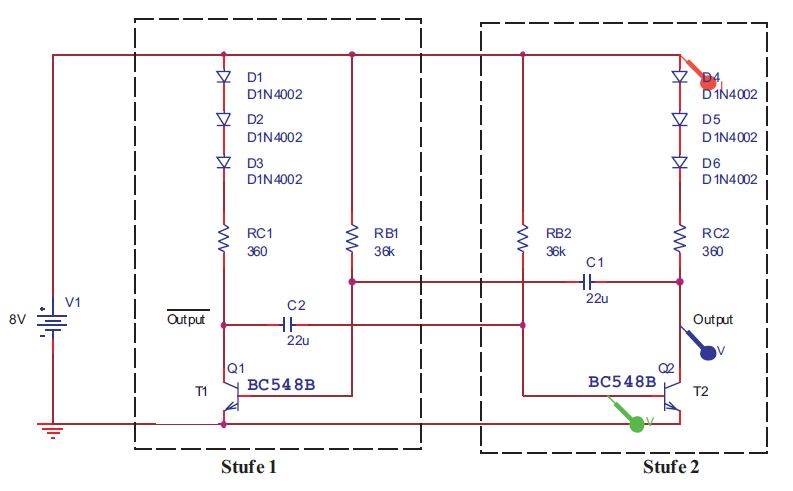
\includegraphics[width = 0.8\textwidth]{\figpath/Astabile_Kippschaltung_Schem.jpg}
    \caption{Astabile Kippschaltung}
    \label{fig_Kap3_01:Astab_Schem}
\end{figure}

\subsection{Analyse der Schaltung}
Die Kollektorwiderstände $R_{C1}$ und $R_{C2}$ begrenzen den Kollektorstrom des Transistors, die Basiswiderstände $R_{B1}$ und $R_{B2}$ müssen ein durchsteuern der Transistoren noch gewährleisten. Zunächst soll der Einschaltvorgang betrachtet werden. Die Schaltung wird vereinfacht (ohne Dioden) in Abb. \ref{fig_Kap3_02:Kipp_ESB} dargestellt. 

\begin{figure}[H]
	\centering
	\def\svgwidth{\textwidth}
	\input{\figpath/Kipp.pdf_tex}
	\caption{Reduziertes ESB der Kippschaltung} 
	\label{fig_Kap3_02:Kipp_ESB} 
\end{figure}


\subsubsection{Einschaltvorgang}
Ohne angelegter Versorgungsspannung sind die Kondensatoren $C_1$ und $C_2$ zunächst entladen, die Transistoren $T_1$ und $T_2$ sperren. Wird nun eine Betriebsspannung $U_B$ angelegt, fließt Strom einerseits über $R_{C1}$, $C_2$ und parallel durch $R_{B2}$ zur Basis von $T_2$, andererseits über $R_{C2}$, $C_1$ und parallel durch $R_{B1}$ zur Basis von $T_1$. Bauteiltoleranzen führen dazu, dass ein Transistor vor dem anderen durchschaltet. Zur einfacheren Erklärung wird nun die $T_1$ verbunden und sei zu diesem Zeitpunkt noch nicht geladen, wodurch das Potential der Basis von $T_2$ Richtung Masse gezogen wird und somit $T_2$ sperrt. Der Transistor $T_1$ bezieht seinen Basisstrom von $R_{B1}$ und $C_1$. Sollte sich $C_1$ bereits aufgeladen haben, liegt an seinen Klemmen ca. $U_B - U_{BE,1}$ an, da ja gilt: $I_{C2} = 0$. In der Zwischenzeit wird der Kondensator $C_2$ solange über den Widerstand $R_{B2}$ geladen, bis an der Basis von $T_2$ die Basis-Emitter-Durchlassspannung erreicht wird ($U_{BE,2} \approx 0,7$ V). Da die Kondensatoren zu diesem Zeitpunkt noch nicht vollständig geladen sind ist dieser Einschaltvorgang, wie sich auch in der Simulation zeigen wird, von kürzerer Dauer, als die Umschaltzeiten des eigentlichen periodischen Verhaltens.

\subsubsection{Periodisches Verhalten}
Zustand $T_1$ leitet: \\
Vor diesem Zustand war $T_1$ sperrend, womit $U_{CE,1}$ ungefähr $U_B$ betrug. Leitet nun $T_1$ sinkt die Kollektor-Emitterspannung auf $U_{CE,1,sat}$. Das Potential der kollektorseitigen Elektrode des Kondensators $C_2$ sinkt nun ebenso um $U_B - U_{CE,1,sat}$. Die Spannung an der gegenüberliegenden Elektrode von $C_2$, mit der Basis von $T_2$ verbunden, sinkt nun ebenso um denselben Betrag, da ja die Spannung am Kondensator bekanntlich nicht springen kann. Davor war $T_2$ leitend womit an dieser Elektrode die Durchlassspannung von ca. 0,7 V wirkte. Somit sinkt die Spannung an der Basis von $T_2$ um

\begin{equation}
U_{BE,2} \approx 0,7 - (U_B - U_{CE,1,sat}) = -U_B + U_{CE,1,sat} + 0,7 .
\end{equation}

Die Versorgungsspannung ist größer als die Sättigungs- und Durchlassspannungen am Transistor, womit die Basis-Emitterspannung negativ wird und $T_2$ sicher sperrt. Mit anderen Worten, die Polarität des Kondensators $C_2$ hat sich sprunghaft geändert. Das Potential an der kollektorseitigen Elektrode ist nun geringer als an der basisseitigen. Es startet ein Umladevorgang. $C_2$ lädt sich über $R_{B2}$ so lange auf, bis an der Basis von $T_2$ wieder jene Basis-Emitter-Durchlassspannung wirkt.

Zustand $T_2$ leitet: \\
Die Vorgänge finden umgekehrt zum vorhergehend erklärten Zustand statt. Die Kollektor-Emitterspannung von $T_2$ sinkt auf $U_{CE,2,sat}$, womit die Spannungen an den Klemmen von $C_1$ um $U_B - U_{CE,1,sat}$ sinken. 

\begin{equation}
U_{BE,1} \approx 0,7 - (U_B - U_{CE,2,sat}) = -U_B + U_{CE,2,sat} + 0,7 .
\end{equation}

Aufgrund der negativen Basis-Emitterspannung sperrt $T_1$ sicher. Nun wird $C_1$ über $R_{B1}$ geladen, bis $U_{BE,1} \approx 0,7$V gilt.

\subsubsection{Periodendauer}
Wann die Schaltungen die Zustände wechseln hängt somit von den Zeitkonstanten beider RC-Glieder ab.

\begin{equation}
    \tau_1 = R_{B1} \cdot C_1
\end{equation}

\begin{equation}
    \tau_2 = R_{B2} \cdot C_2
\end{equation}

Der Umladevorgang am Kondensator kann folgendermaßen beschrieben werden

\begin{equation}
    U_{C}(t) = U_{end} + (U_{start} - U_{end}) \cdot e^{-\frac{t}{\tau}}.
\end{equation}

Vernachlässigt man die Kollektor-Emitter-Sättigungsspannung gegenüber der Versorgungsspannung gilt

\begin{equation}
    U_{end} = U_B
\end{equation}

und 

\begin{equation}
    U_{start} = -U_B .
\end{equation}

Trifft man weiters die vereinfachende Annahme, dass der Transistor ab einer Basisspannung von 0V leitet, folgt

\begin{equation}
    U_{C}(T) = 0 = U_B - 2 U_B \cdot e^{-\frac{T}{\tau}}
\end{equation}

\begin{equation}
    \frac{1}{2} = e^{-\frac{T}{\tau}}
\end{equation}

\begin{equation}
    T = \text{ln}(2) \cdot \tau
\end{equation}

Die gesamte Periodendauer der betrachteten Kippschaltung bestimmt sich somit aus jener Zeitdauer, wo der Transistor $T_1$ leitet, 

\begin{equation}
    T_1 \approx \text{ln}(2) \cdot R_{B2}C_2 ,
\end{equation}

und jener wo Transistor $T_2$ leitet

\begin{equation}
    T_2 \approx \text{ln}(2) \cdot R_{B1}C_1 .
\end{equation}

Die betrachtete Schaltung ist symmetrisch, woraus sich eine Periodendauer von

\begin{equation}
    \label{glgn:period}
    T \approx 2 \cdot \text{ln}(2) \cdot R_{B1}C_1 = 2 \cdot \text{ln}(2) \cdot \SI{36}{\kilo\ohm} \cdot \SI{22}{\micro\farad} = \SI{1.098}{\second}
\end{equation}

ergibt.

Eine LED leuchtet für jene Dauer, in der ein bestimmter Transistor leitet, was bei der symmetrischen Schaltung die halbe Periode ist,

\begin{equation}
    T_{1,2} \approx \text{ln}(2) \cdot R_{B1}C_1 = 2 \cdot \text{ln}(2) \cdot \SI{36}{\kilo\ohm} \cdot \SI{22}{\micro\farad} = \SI{0.549}{\second}.
\end{equation}


\subsection{Simulation}
Die Schaltung wurde in LTSpice simuliert. Das zugehörige Schematic kann in Abb. \ref{fig_Kap3_03:LTSpice_Schem_1} betrachtet werden.

\begin{figure}[H]
    \centering
    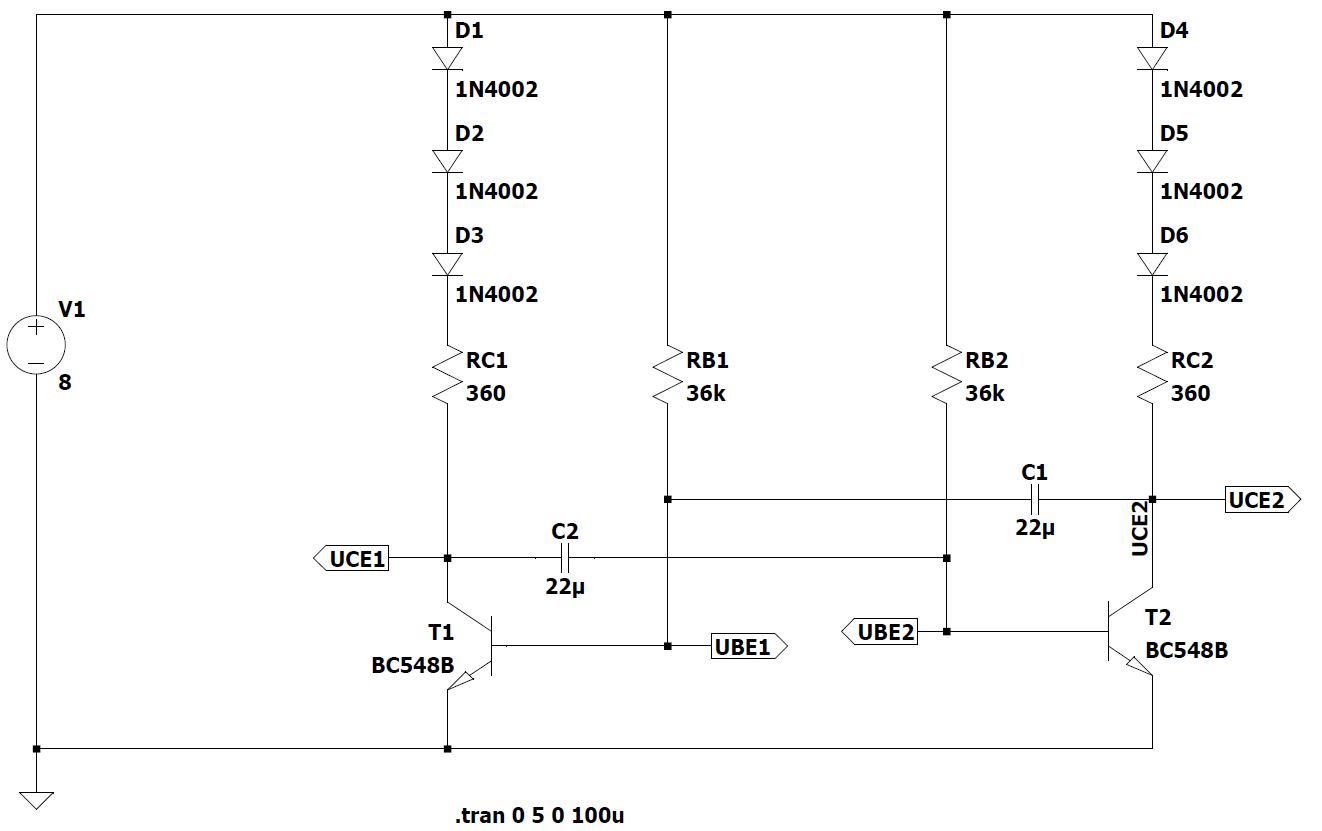
\includegraphics[width = 0.8\textwidth]{\figpath/Kipp_schem_1.jpg}
    \caption{Astabile Kippschaltung in LTSpice}
    \label{fig_Kap3_03:LTSpice_Schem_1}
\end{figure}

Es wurde eine 5 Sekunden lang eine Transientensimulation mit einem Zeitschritt von $0.1$ms durchgeführt.

\begin{figure}[H]
	\centering \small
	\scalebox{0.9}{% This file was created by matlab2tikz.
%
\definecolor{mycolor1}{rgb}{0.00000,0.44700,0.74100}%
\definecolor{mycolor2}{rgb}{0.85000,0.32500,0.09800}%
\definecolor{mycolor3}{rgb}{0.92900,0.69400,0.12500}%
\definecolor{mycolor4}{rgb}{0.49400,0.18400,0.55600}%
%
\begin{tikzpicture}

\begin{axis}[%
width=4.521in,
height=3.566in,
at={(0.758in,0.481in)},
scale only axis,
xmin=0,
xmax=250,
xlabel style={font=\color{white!15!black}},
xlabel={$t \text{ in s}$},
ymin=-6,
ymax=8,
ylabel style={font=\color{white!15!black}},
ylabel={$V \text{ in V}$},
axis background/.style={fill=white},
title style={font=\bfseries},
title={Einschaltvorgang},
xmajorgrids,
ymajorgrids,
legend style={at={(0.03,0.03)}, anchor=south west, legend cell align=left, align=left, draw=white!15!black}
]
\addplot [color=mycolor1, forget plot]
  table[row sep=crcr]{%
0	0.741\\
1	0.741\\
2	0.741\\
3	0.741\\
4	0.741\\
5	0.741\\
6	0.741\\
7	0.741\\
8	0.741\\
9	0.741\\
10	0.741\\
11	0.741\\
12	0.741\\
13	0.741\\
14	0.741\\
15	0.741\\
16	0.741\\
17	0.741\\
18	0.741\\
19	0.741\\
20	0.741\\
21	0.741\\
22	0.741\\
23	0.741\\
24	0.741\\
25	0.741\\
26	0.741\\
27	0.741\\
28	0.741\\
29	0.741\\
30	0.741\\
31	0.741\\
32	0.741\\
33	0.741\\
34	0.741\\
35	0.741\\
36	0.741\\
37	0.741\\
38	0.741\\
39	0.741\\
40	0.741\\
41	0.741\\
42	0.741\\
43	0.741\\
44	0.741\\
45	0.741\\
46	0.741\\
47	0.741\\
48	0.741\\
49	0.741\\
50	0.741\\
51	0.741\\
52	0.741\\
53	0.741\\
54	0.741\\
55	0.741\\
56	0.741\\
57	0.741\\
58	0.741\\
59	0.741\\
60	0.741\\
61	0.741\\
62	0.741\\
63	0.741\\
64	0.741\\
65	0.741\\
66	0.741\\
67	0.741\\
68	0.741\\
69	0.741\\
70	0.741\\
71	0.741\\
72	0.741\\
73	0.741\\
74	0.741\\
75	0.741\\
76	0.741\\
77	0.741\\
78	0.741\\
79	0.741\\
80	0.741\\
81	0.741\\
82	0.741\\
83	0.741\\
84	0.741\\
85	0.741\\
86	0.741\\
87	0.741\\
88	0.741\\
89	0.741\\
90	0.741\\
91	0.741\\
92	0.741\\
93	0.741\\
94	0.741\\
95	0.741\\
96	0.741\\
97	0.741\\
98	0.741\\
99	0.741\\
100	0.741\\
101	0.741\\
102	0.741\\
103	0.741\\
104	0.742\\
105	0.742\\
106	0.742\\
107	0.743\\
108	0.744\\
109	0.745\\
110	0.747\\
111	0.751\\
112	0.316\\
113	0.326\\
114	0.337\\
115	0.348\\
116	0.359\\
117	0.369\\
118	0.381\\
119	0.392\\
120	0.403\\
121	0.414\\
122	0.425\\
123	0.437\\
124	0.448\\
125	0.459\\
126	0.471\\
127	0.482\\
128	0.494\\
129	0.505\\
130	0.516\\
131	0.528\\
132	0.539\\
133	0.55\\
134	0.562\\
135	0.573\\
136	0.585\\
137	0.596\\
138	0.608\\
139	0.621\\
140	0.642\\
141	0.769\\
142	0.767\\
143	0.765\\
144	0.763\\
145	0.762\\
146	0.76\\
147	0.758\\
148	0.757\\
149	0.755\\
150	0.754\\
151	0.753\\
152	0.752\\
153	0.751\\
154	0.75\\
155	0.75\\
156	0.749\\
157	0.748\\
158	0.748\\
159	0.747\\
160	0.747\\
161	0.746\\
162	0.746\\
163	0.745\\
164	0.745\\
165	0.745\\
166	0.745\\
167	0.744\\
168	0.744\\
169	0.744\\
170	0.744\\
171	0.744\\
172	0.743\\
173	0.743\\
174	0.743\\
175	0.743\\
176	0.743\\
177	0.743\\
178	0.743\\
179	0.743\\
180	0.743\\
181	0.743\\
182	0.743\\
183	0.743\\
184	0.742\\
185	0.742\\
186	0.742\\
187	0.742\\
188	0.742\\
189	0.742\\
190	0.742\\
191	0.742\\
192	0.742\\
193	0.742\\
194	0.742\\
195	0.742\\
196	0.742\\
197	0.742\\
198	0.742\\
199	0.742\\
200	0.742\\
201	0.742\\
202	0.742\\
203	0.742\\
204	0.742\\
205	0.742\\
206	0.742\\
207	0.742\\
208	0.742\\
209	0.742\\
210	0.742\\
211	0.742\\
212	0.742\\
213	0.742\\
214	0.742\\
215	0.742\\
216	0.742\\
217	0.742\\
218	0.742\\
219	0.742\\
220	0.742\\
221	0.742\\
222	0.742\\
223	0.742\\
224	0.742\\
225	0.742\\
226	0.742\\
227	0.742\\
228	0.742\\
229	0.742\\
230	0.742\\
231	0.742\\
232	0.742\\
233	0.742\\
234	0.742\\
235	0.742\\
236	0.742\\
237	0.742\\
238	0.742\\
239	0.742\\
240	0.742\\
241	0.742\\
242	0.742\\
243	0.742\\
244	0.742\\
245	0.742\\
246	0.742\\
247	0.742\\
248	0.742\\
249	0.742\\
250	0.742\\
251	0.742\\
252	0.742\\
253	0.742\\
254	0.742\\
255	0.742\\
256	0.742\\
257	0.742\\
258	0.742\\
259	0.742\\
260	0.742\\
261	0.742\\
262	0.742\\
263	0.742\\
264	0.742\\
265	0.742\\
266	0.742\\
267	0.742\\
268	0.742\\
269	0.742\\
270	0.742\\
271	0.742\\
272	0.742\\
273	0.742\\
274	0.742\\
275	0.741\\
276	0.741\\
277	0.741\\
278	0.741\\
279	0.741\\
280	0.741\\
281	0.741\\
282	0.741\\
283	0.741\\
284	0.741\\
285	0.741\\
286	0.741\\
287	0.741\\
288	0.741\\
289	0.741\\
290	0.741\\
291	0.741\\
292	0.741\\
293	0.741\\
294	0.741\\
295	0.741\\
296	0.741\\
297	0.741\\
298	0.741\\
299	0.741\\
300	0.741\\
301	0.741\\
302	0.741\\
303	0.741\\
304	0.741\\
305	0.741\\
306	0.741\\
307	0.741\\
308	0.741\\
309	0.741\\
310	0.741\\
311	0.741\\
312	0.741\\
313	0.741\\
314	0.741\\
315	0.741\\
316	0.741\\
317	0.741\\
318	0.741\\
319	0.741\\
320	0.741\\
321	0.741\\
322	0.741\\
323	0.741\\
324	0.741\\
325	0.741\\
326	0.741\\
327	0.741\\
328	0.741\\
329	0.741\\
330	0.741\\
331	0.741\\
332	0.741\\
333	0.741\\
334	0.741\\
335	0.741\\
336	0.741\\
337	0.741\\
338	0.741\\
339	0.741\\
340	0.741\\
341	0.741\\
342	0.741\\
343	0.741\\
344	0.741\\
345	0.741\\
346	0.741\\
347	0.741\\
348	0.741\\
349	0.741\\
350	0.741\\
351	0.741\\
352	0.741\\
353	0.741\\
354	0.741\\
355	0.741\\
356	0.741\\
357	0.741\\
358	0.741\\
359	0.741\\
360	0.741\\
361	0.741\\
362	0.741\\
363	0.741\\
364	0.741\\
365	0.741\\
366	0.741\\
367	0.741\\
368	0.741\\
369	0.741\\
370	0.741\\
371	0.741\\
372	0.741\\
373	0.741\\
374	0.741\\
375	0.741\\
376	0.741\\
377	0.741\\
378	0.741\\
379	0.741\\
380	0.741\\
381	0.741\\
382	0.741\\
383	0.741\\
384	0.741\\
385	0.741\\
386	0.741\\
387	0.741\\
388	0.741\\
389	0.741\\
390	0.741\\
391	0.741\\
392	0.741\\
393	0.741\\
394	0.741\\
395	0.741\\
396	0.741\\
397	0.741\\
398	0.741\\
399	0.741\\
400	0.741\\
401	0.741\\
402	0.741\\
403	0.741\\
404	0.741\\
405	0.741\\
406	0.741\\
407	0.741\\
408	0.741\\
409	0.741\\
410	0.741\\
411	0.741\\
412	0.741\\
413	0.741\\
414	0.741\\
415	0.741\\
416	0.741\\
417	0.741\\
418	0.741\\
419	0.741\\
420	0.741\\
421	0.741\\
422	0.741\\
423	0.741\\
424	0.741\\
425	0.741\\
426	0.741\\
427	0.741\\
428	0.741\\
429	0.741\\
430	0.741\\
431	0.741\\
432	0.741\\
433	0.741\\
434	0.741\\
435	0.741\\
436	0.741\\
437	0.741\\
438	0.741\\
439	0.741\\
440	0.741\\
441	0.741\\
442	0.741\\
443	0.741\\
444	0.741\\
445	0.741\\
446	0.741\\
447	0.741\\
448	0.741\\
449	0.741\\
450	0.741\\
451	0.741\\
452	0.741\\
453	0.741\\
454	0.741\\
455	0.741\\
456	0.741\\
457	0.741\\
458	0.741\\
459	0.741\\
460	0.741\\
461	0.741\\
462	0.741\\
463	0.741\\
464	0.741\\
465	0.741\\
466	0.741\\
467	0.741\\
468	0.741\\
469	0.741\\
470	0.741\\
471	0.741\\
472	0.741\\
473	0.741\\
474	0.741\\
475	0.741\\
476	0.741\\
477	0.741\\
478	0.741\\
479	0.741\\
480	0.741\\
481	0.741\\
482	0.741\\
483	0.741\\
484	0.741\\
485	0.741\\
486	0.741\\
487	0.741\\
488	0.741\\
489	0.741\\
490	0.741\\
491	0.741\\
492	0.741\\
493	0.741\\
494	0.741\\
495	0.741\\
496	0.741\\
497	0.741\\
498	0.741\\
499	0.741\\
500	0.741\\
501	0.741\\
502	0.741\\
503	0.741\\
504	0.741\\
505	0.741\\
506	0.741\\
507	0.741\\
508	0.741\\
509	0.741\\
510	0.741\\
511	0.741\\
512	0.741\\
513	0.741\\
514	0.741\\
515	0.741\\
516	0.741\\
517	0.741\\
518	0.741\\
519	0.741\\
520	0.741\\
521	0.741\\
522	0.741\\
523	0.741\\
524	0.741\\
525	0.741\\
526	0.741\\
527	0.741\\
528	0.741\\
529	0.741\\
530	0.741\\
531	0.741\\
532	0.741\\
533	0.741\\
534	0.741\\
535	0.741\\
536	0.741\\
537	0.741\\
538	0.741\\
539	0.741\\
540	0.741\\
541	0.741\\
542	0.741\\
543	0.741\\
544	0.741\\
545	0.741\\
546	0.741\\
547	0.741\\
548	0.741\\
549	0.741\\
550	0.741\\
551	0.741\\
552	0.741\\
553	0.741\\
554	0.741\\
555	0.741\\
556	0.741\\
557	0.741\\
558	0.741\\
559	0.741\\
560	0.741\\
561	0.741\\
562	0.741\\
563	0.741\\
564	0.741\\
565	0.741\\
566	0.741\\
567	0.741\\
568	0.741\\
569	0.741\\
570	0.741\\
571	0.741\\
572	0.741\\
573	0.741\\
574	0.741\\
575	0.741\\
576	0.741\\
577	0.741\\
578	0.741\\
579	0.741\\
580	0.741\\
581	0.741\\
582	0.741\\
583	0.741\\
584	0.741\\
585	0.741\\
586	0.741\\
587	0.741\\
588	0.741\\
589	0.741\\
590	0.741\\
591	0.741\\
592	0.741\\
593	-6.2\\
594	-6.181\\
595	-6.163\\
596	-6.144\\
597	-6.124\\
598	-6.105\\
599	-6.086\\
600	-6.067\\
601	-6.047\\
602	-6.028\\
603	-6.009\\
604	-5.989\\
605	-5.97\\
606	-5.95\\
607	-5.931\\
608	-5.911\\
609	-5.892\\
610	-5.872\\
611	-5.853\\
612	-5.834\\
613	-5.814\\
614	-5.795\\
615	-5.776\\
616	-5.757\\
617	-5.737\\
618	-5.718\\
619	-5.699\\
620	-5.68\\
621	-5.662\\
622	-5.643\\
623	-5.624\\
624	-5.606\\
625	-5.587\\
626	-5.569\\
627	-5.55\\
628	-5.532\\
629	-5.514\\
630	-5.496\\
631	-5.478\\
632	-5.46\\
633	-5.442\\
634	-5.424\\
635	-5.406\\
636	-5.388\\
637	-5.371\\
638	-5.353\\
639	-5.335\\
640	-5.318\\
641	-5.3\\
642	-5.283\\
643	-5.266\\
644	-5.248\\
645	-5.231\\
646	-5.214\\
647	-5.197\\
648	-5.179\\
649	-5.162\\
650	-5.145\\
651	-5.128\\
652	-5.111\\
653	-5.094\\
654	-5.077\\
655	-5.061\\
656	-5.044\\
657	-5.027\\
658	-5.01\\
659	-4.993\\
660	-4.977\\
661	-4.96\\
662	-4.943\\
663	-4.927\\
664	-4.91\\
665	-4.894\\
666	-4.877\\
667	-4.861\\
668	-4.844\\
669	-4.828\\
670	-4.811\\
671	-4.795\\
672	-4.779\\
673	-4.762\\
674	-4.746\\
675	-4.73\\
676	-4.714\\
677	-4.697\\
678	-4.681\\
679	-4.665\\
680	-4.649\\
681	-4.633\\
682	-4.617\\
683	-4.601\\
684	-4.585\\
685	-4.569\\
686	-4.553\\
687	-4.537\\
688	-4.521\\
689	-4.505\\
690	-4.489\\
691	-4.473\\
692	-4.457\\
693	-4.441\\
694	-4.425\\
695	-4.41\\
696	-4.394\\
697	-4.378\\
698	-4.362\\
699	-4.347\\
700	-4.331\\
701	-4.315\\
702	-4.3\\
703	-4.284\\
704	-4.269\\
705	-4.253\\
706	-4.237\\
707	-4.222\\
708	-4.206\\
709	-4.191\\
710	-4.175\\
711	-4.16\\
712	-4.145\\
713	-4.129\\
714	-4.114\\
715	-4.098\\
716	-4.083\\
717	-4.068\\
718	-4.053\\
719	-4.037\\
720	-4.022\\
721	-4.007\\
722	-3.992\\
723	-3.976\\
724	-3.961\\
725	-3.946\\
726	-3.931\\
727	-3.916\\
728	-3.901\\
729	-3.886\\
730	-3.871\\
731	-3.856\\
732	-3.841\\
733	-3.826\\
734	-3.811\\
735	-3.796\\
736	-3.781\\
737	-3.766\\
738	-3.751\\
739	-3.736\\
740	-3.721\\
741	-3.706\\
742	-3.692\\
743	-3.677\\
744	-3.662\\
745	-3.647\\
746	-3.632\\
747	-3.618\\
748	-3.603\\
749	-3.588\\
750	-3.574\\
751	-3.559\\
752	-3.544\\
753	-3.53\\
754	-3.515\\
755	-3.501\\
756	-3.486\\
757	-3.472\\
758	-3.457\\
759	-3.443\\
760	-3.428\\
761	-3.414\\
762	-3.399\\
763	-3.385\\
764	-3.37\\
765	-3.356\\
766	-3.342\\
767	-3.327\\
768	-3.313\\
769	-3.299\\
770	-3.284\\
771	-3.27\\
772	-3.256\\
773	-3.242\\
774	-3.228\\
775	-3.213\\
776	-3.199\\
777	-3.185\\
778	-3.171\\
779	-3.157\\
780	-3.143\\
781	-3.129\\
782	-3.114\\
783	-3.1\\
784	-3.086\\
785	-3.072\\
786	-3.058\\
787	-3.044\\
788	-3.03\\
789	-3.017\\
790	-3.003\\
791	-2.989\\
792	-2.975\\
793	-2.961\\
794	-2.947\\
795	-2.933\\
796	-2.919\\
797	-2.906\\
798	-2.892\\
799	-2.878\\
800	-2.864\\
801	-2.851\\
802	-2.837\\
803	-2.823\\
804	-2.81\\
805	-2.796\\
806	-2.782\\
807	-2.769\\
808	-2.755\\
809	-2.742\\
810	-2.728\\
811	-2.714\\
812	-2.701\\
813	-2.687\\
814	-2.674\\
815	-2.66\\
816	-2.647\\
817	-2.633\\
818	-2.62\\
819	-2.607\\
820	-2.593\\
821	-2.58\\
822	-2.566\\
823	-2.553\\
824	-2.54\\
825	-2.526\\
826	-2.513\\
827	-2.5\\
828	-2.487\\
829	-2.473\\
830	-2.46\\
831	-2.447\\
832	-2.434\\
833	-2.42\\
834	-2.407\\
835	-2.394\\
836	-2.381\\
837	-2.368\\
838	-2.355\\
839	-2.342\\
840	-2.329\\
841	-2.316\\
842	-2.303\\
843	-2.29\\
844	-2.277\\
845	-2.264\\
846	-2.251\\
847	-2.238\\
848	-2.225\\
849	-2.212\\
850	-2.199\\
851	-2.186\\
852	-2.173\\
853	-2.16\\
854	-2.147\\
855	-2.135\\
856	-2.122\\
857	-2.109\\
858	-2.096\\
859	-2.084\\
860	-2.071\\
861	-2.058\\
862	-2.045\\
863	-2.033\\
864	-2.02\\
865	-2.007\\
866	-1.995\\
867	-1.982\\
868	-1.97\\
869	-1.957\\
870	-1.944\\
871	-1.932\\
872	-1.919\\
873	-1.907\\
874	-1.894\\
875	-1.882\\
876	-1.869\\
877	-1.857\\
878	-1.844\\
879	-1.832\\
880	-1.82\\
881	-1.807\\
882	-1.795\\
883	-1.782\\
884	-1.77\\
885	-1.758\\
886	-1.745\\
887	-1.733\\
888	-1.721\\
889	-1.709\\
890	-1.696\\
891	-1.684\\
892	-1.672\\
893	-1.66\\
894	-1.647\\
895	-1.635\\
896	-1.623\\
897	-1.611\\
898	-1.599\\
899	-1.587\\
900	-1.575\\
901	-1.563\\
902	-1.55\\
903	-1.538\\
904	-1.526\\
905	-1.514\\
906	-1.502\\
907	-1.49\\
908	-1.478\\
909	-1.466\\
910	-1.455\\
911	-1.443\\
912	-1.431\\
913	-1.419\\
914	-1.407\\
915	-1.395\\
916	-1.383\\
917	-1.371\\
918	-1.359\\
919	-1.348\\
920	-1.336\\
921	-1.324\\
922	-1.312\\
923	-1.301\\
924	-1.289\\
925	-1.277\\
926	-1.265\\
927	-1.254\\
928	-1.242\\
929	-1.23\\
930	-1.219\\
931	-1.207\\
932	-1.195\\
933	-1.184\\
934	-1.172\\
935	-1.161\\
936	-1.149\\
937	-1.137\\
938	-1.126\\
939	-1.114\\
940	-1.103\\
941	-1.091\\
942	-1.08\\
943	-1.068\\
944	-1.057\\
945	-1.046\\
946	-1.034\\
947	-1.023\\
948	-1.011\\
949	-1\\
950	-0.989\\
951	-0.977\\
952	-0.966\\
953	-0.954\\
954	-0.943\\
955	-0.932\\
956	-0.921\\
957	-0.909\\
958	-0.898\\
959	-0.887\\
960	-0.876\\
961	-0.864\\
962	-0.853\\
963	-0.842\\
964	-0.831\\
965	-0.82\\
966	-0.809\\
967	-0.797\\
968	-0.786\\
969	-0.775\\
970	-0.764\\
971	-0.753\\
972	-0.742\\
973	-0.731\\
974	-0.72\\
975	-0.709\\
976	-0.698\\
977	-0.687\\
978	-0.676\\
979	-0.665\\
980	-0.654\\
981	-0.643\\
982	-0.632\\
983	-0.621\\
984	-0.611\\
985	-0.6\\
986	-0.589\\
987	-0.578\\
988	-0.567\\
989	-0.556\\
990	-0.546\\
991	-0.535\\
992	-0.524\\
993	-0.513\\
994	-0.503\\
995	-0.492\\
996	-0.481\\
997	-0.47\\
998	-0.46\\
999	-0.449\\
1000	-0.438\\
1001	-0.428\\
1002	-0.417\\
1003	-0.407\\
1004	-0.396\\
1005	-0.385\\
1006	-0.375\\
1007	-0.364\\
1008	-0.354\\
1009	-0.343\\
1010	-0.333\\
1011	-0.322\\
1012	-0.312\\
1013	-0.301\\
1014	-0.291\\
1015	-0.28\\
1016	-0.27\\
1017	-0.259\\
1018	-0.249\\
1019	-0.238\\
1020	-0.228\\
1021	-0.218\\
1022	-0.207\\
1023	-0.197\\
1024	-0.186\\
1025	-0.176\\
1026	-0.166\\
1027	-0.156\\
1028	-0.145\\
1029	-0.135\\
1030	-0.125\\
1031	-0.114\\
1032	-0.104\\
1033	-0.094\\
1034	-0.084\\
1035	-0.074\\
1036	-0.063\\
1037	-0.053\\
1038	-0.043\\
1039	-0.033\\
1040	-0.023\\
1041	-0.013\\
1042	-0.002\\
1043	0.008\\
1044	0.018\\
1045	0.028\\
1046	0.038\\
1047	0.048\\
1048	0.058\\
1049	0.068\\
1050	0.078\\
1051	0.088\\
1052	0.098\\
1053	0.108\\
1054	0.118\\
1055	0.128\\
1056	0.138\\
1057	0.148\\
1058	0.158\\
1059	0.168\\
1060	0.177\\
1061	0.187\\
1062	0.197\\
1063	0.207\\
1064	0.217\\
1065	0.227\\
1066	0.236\\
1067	0.246\\
1068	0.256\\
1069	0.266\\
1070	0.276\\
1071	0.285\\
1072	0.295\\
1073	0.305\\
1074	0.314\\
1075	0.324\\
1076	0.334\\
1077	0.344\\
1078	0.353\\
1079	0.363\\
1080	0.373\\
1081	0.382\\
1082	0.392\\
1083	0.401\\
1084	0.411\\
1085	0.421\\
1086	0.43\\
1087	0.44\\
1088	0.449\\
1089	0.459\\
1090	0.468\\
1091	0.478\\
1092	0.487\\
1093	0.497\\
1094	0.507\\
1095	0.516\\
1096	0.526\\
1097	0.536\\
1098	0.546\\
1099	0.556\\
1100	0.567\\
1101	0.58\\
1102	0.77\\
1103	0.768\\
1104	0.766\\
1105	0.764\\
1106	0.762\\
1107	0.761\\
1108	0.759\\
1109	0.758\\
1110	0.756\\
1111	0.755\\
1112	0.754\\
1113	0.753\\
1114	0.752\\
1115	0.751\\
1116	0.75\\
1117	0.749\\
1118	0.748\\
1119	0.748\\
1120	0.747\\
1121	0.747\\
1122	0.746\\
1123	0.746\\
1124	0.746\\
1125	0.745\\
1126	0.745\\
1127	0.745\\
1128	0.744\\
1129	0.744\\
1130	0.744\\
1131	0.744\\
1132	0.744\\
1133	0.744\\
1134	0.743\\
1135	0.743\\
1136	0.743\\
1137	0.743\\
1138	0.743\\
1139	0.743\\
1140	0.743\\
1141	0.743\\
1142	0.743\\
1143	0.743\\
1144	0.743\\
1145	0.743\\
1146	0.742\\
1147	0.742\\
1148	0.742\\
1149	0.742\\
1150	0.742\\
1151	0.742\\
1152	0.742\\
1153	0.742\\
1154	0.742\\
1155	0.742\\
1156	0.742\\
1157	0.742\\
1158	0.742\\
1159	0.742\\
1160	0.742\\
1161	0.742\\
1162	0.742\\
1163	0.742\\
1164	0.742\\
1165	0.742\\
1166	0.742\\
1167	0.742\\
1168	0.742\\
1169	0.742\\
1170	0.742\\
1171	0.742\\
1172	0.742\\
1173	0.742\\
1174	0.742\\
1175	0.742\\
1176	0.742\\
1177	0.742\\
1178	0.742\\
1179	0.742\\
1180	0.742\\
1181	0.742\\
1182	0.742\\
1183	0.742\\
1184	0.742\\
1185	0.742\\
1186	0.742\\
1187	0.742\\
1188	0.742\\
1189	0.742\\
1190	0.742\\
1191	0.742\\
1192	0.742\\
1193	0.742\\
1194	0.742\\
1195	0.742\\
1196	0.742\\
1197	0.742\\
1198	0.742\\
1199	0.742\\
1200	0.742\\
1201	0.742\\
1202	0.742\\
1203	0.742\\
1204	0.742\\
1205	0.742\\
1206	0.742\\
1207	0.742\\
1208	0.742\\
1209	0.742\\
1210	0.742\\
1211	0.742\\
1212	0.742\\
1213	0.742\\
1214	0.742\\
1215	0.742\\
1216	0.742\\
1217	0.742\\
1218	0.742\\
1219	0.742\\
1220	0.742\\
1221	0.742\\
1222	0.742\\
1223	0.742\\
1224	0.742\\
1225	0.742\\
1226	0.742\\
1227	0.742\\
1228	0.742\\
1229	0.742\\
1230	0.742\\
1231	0.742\\
1232	0.742\\
1233	0.742\\
1234	0.742\\
1235	0.742\\
1236	0.742\\
1237	0.742\\
1238	0.742\\
1239	0.742\\
1240	0.742\\
1241	0.742\\
1242	0.742\\
1243	0.742\\
1244	0.742\\
1245	0.742\\
1246	0.742\\
1247	0.742\\
1248	0.742\\
1249	0.742\\
1250	0.742\\
1251	0.742\\
1252	0.742\\
1253	0.742\\
1254	0.742\\
1255	0.742\\
1256	0.741\\
1257	0.741\\
1258	0.741\\
1259	0.741\\
1260	0.741\\
1261	0.741\\
1262	0.741\\
1263	0.741\\
1264	0.741\\
1265	0.741\\
1266	0.741\\
1267	0.741\\
1268	0.741\\
1269	0.741\\
1270	0.741\\
1271	0.741\\
1272	0.741\\
1273	0.741\\
1274	0.741\\
1275	0.741\\
1276	0.741\\
1277	0.741\\
1278	0.741\\
1279	0.741\\
1280	0.741\\
1281	0.741\\
1282	0.741\\
1283	0.741\\
1284	0.741\\
1285	0.741\\
1286	0.741\\
1287	0.741\\
1288	0.741\\
1289	0.741\\
1290	0.741\\
1291	0.741\\
1292	0.741\\
1293	0.741\\
1294	0.741\\
1295	0.741\\
1296	0.741\\
1297	0.741\\
1298	0.741\\
1299	0.741\\
1300	0.741\\
1301	0.741\\
1302	0.741\\
1303	0.741\\
1304	0.741\\
1305	0.741\\
1306	0.741\\
1307	0.741\\
1308	0.741\\
1309	0.741\\
1310	0.741\\
1311	0.741\\
1312	0.741\\
1313	0.741\\
1314	0.741\\
1315	0.741\\
1316	0.741\\
1317	0.741\\
1318	0.741\\
1319	0.741\\
1320	0.741\\
1321	0.741\\
1322	0.741\\
1323	0.741\\
1324	0.741\\
1325	0.741\\
1326	0.741\\
1327	0.741\\
1328	0.741\\
1329	0.741\\
1330	0.741\\
1331	0.741\\
1332	0.741\\
1333	0.741\\
1334	0.741\\
1335	0.741\\
1336	0.741\\
1337	0.741\\
1338	0.741\\
1339	0.741\\
1340	0.741\\
1341	0.741\\
1342	0.741\\
1343	0.741\\
1344	0.741\\
1345	0.741\\
1346	0.741\\
1347	0.741\\
1348	0.741\\
1349	0.741\\
1350	0.741\\
1351	0.741\\
1352	0.741\\
1353	0.741\\
1354	0.741\\
1355	0.741\\
1356	0.741\\
1357	0.741\\
1358	0.741\\
1359	0.741\\
1360	0.741\\
1361	0.741\\
1362	0.741\\
1363	0.741\\
1364	0.741\\
1365	0.741\\
1366	0.741\\
1367	0.741\\
1368	0.741\\
1369	0.741\\
1370	0.741\\
1371	0.741\\
1372	0.741\\
1373	0.741\\
1374	0.741\\
1375	0.741\\
1376	0.741\\
1377	0.741\\
1378	0.741\\
1379	0.741\\
1380	0.741\\
1381	0.741\\
1382	0.741\\
1383	0.741\\
1384	0.741\\
1385	0.741\\
1386	0.741\\
1387	0.741\\
1388	0.741\\
1389	0.741\\
1390	0.741\\
1391	0.741\\
1392	0.741\\
1393	0.741\\
1394	0.741\\
1395	0.741\\
1396	0.741\\
1397	0.741\\
1398	0.741\\
1399	0.741\\
1400	0.741\\
1401	0.741\\
1402	0.741\\
1403	0.741\\
1404	0.741\\
1405	0.741\\
1406	0.741\\
1407	0.741\\
1408	0.741\\
1409	0.741\\
1410	0.741\\
1411	0.741\\
1412	0.741\\
1413	0.741\\
1414	0.741\\
1415	0.741\\
1416	0.741\\
1417	0.741\\
1418	0.741\\
1419	0.741\\
1420	0.741\\
1421	0.741\\
1422	0.741\\
1423	0.741\\
1424	0.741\\
1425	0.741\\
1426	0.741\\
1427	0.741\\
1428	0.741\\
1429	0.741\\
1430	0.741\\
1431	0.741\\
1432	0.741\\
1433	0.741\\
1434	0.741\\
1435	0.741\\
1436	0.741\\
1437	0.741\\
1438	0.741\\
1439	0.741\\
1440	0.741\\
1441	0.741\\
1442	0.741\\
1443	0.741\\
1444	0.741\\
1445	0.741\\
1446	0.741\\
1447	0.741\\
1448	0.741\\
1449	0.741\\
1450	0.741\\
1451	0.741\\
1452	0.741\\
1453	0.741\\
1454	0.741\\
1455	0.741\\
1456	0.741\\
1457	0.741\\
1458	0.741\\
1459	0.741\\
1460	0.741\\
1461	0.741\\
1462	0.741\\
1463	0.741\\
1464	0.741\\
1465	0.741\\
1466	0.741\\
1467	0.741\\
1468	0.741\\
1469	0.741\\
1470	0.741\\
1471	0.741\\
1472	0.741\\
1473	0.741\\
1474	0.741\\
1475	0.741\\
1476	0.741\\
1477	0.741\\
1478	0.741\\
1479	0.741\\
1480	0.741\\
1481	0.741\\
1482	0.741\\
1483	0.741\\
1484	0.741\\
1485	0.741\\
1486	0.741\\
1487	0.741\\
1488	0.741\\
1489	0.741\\
1490	0.741\\
1491	0.741\\
1492	0.741\\
1493	0.741\\
1494	0.741\\
1495	0.741\\
1496	0.741\\
1497	0.741\\
1498	0.741\\
1499	0.741\\
1500	0.741\\
1501	0.741\\
1502	0.741\\
1503	0.741\\
1504	0.741\\
1505	0.741\\
1506	0.741\\
1507	0.741\\
1508	0.741\\
1509	0.741\\
1510	0.741\\
1511	0.741\\
1512	0.741\\
1513	0.741\\
1514	0.741\\
1515	0.741\\
1516	0.741\\
1517	0.741\\
1518	0.741\\
1519	0.741\\
1520	0.741\\
1521	0.741\\
1522	0.741\\
1523	0.741\\
1524	0.741\\
1525	0.741\\
1526	0.741\\
1527	0.741\\
1528	0.741\\
1529	0.741\\
1530	0.741\\
1531	0.741\\
1532	0.741\\
1533	0.741\\
1534	0.741\\
1535	0.741\\
1536	0.741\\
1537	0.741\\
1538	0.741\\
1539	0.741\\
1540	0.741\\
1541	0.741\\
1542	0.741\\
1543	0.741\\
1544	0.741\\
1545	0.741\\
1546	0.741\\
1547	0.741\\
1548	0.741\\
1549	0.741\\
1550	0.741\\
1551	0.741\\
1552	0.741\\
1553	0.741\\
1554	0.741\\
1555	0.741\\
1556	0.741\\
1557	0.741\\
1558	0.741\\
1559	0.741\\
1560	0.741\\
1561	0.741\\
1562	0.741\\
1563	0.741\\
1564	0.741\\
1565	0.741\\
1566	0.741\\
1567	0.741\\
1568	0.741\\
1569	0.741\\
1570	0.741\\
1571	0.741\\
1572	0.741\\
1573	0.741\\
1574	0.741\\
1575	0.741\\
1576	0.741\\
1577	0.741\\
1578	0.741\\
1579	0.741\\
1580	0.741\\
1581	0.741\\
1582	0.741\\
1583	0.741\\
1584	0.741\\
1585	0.741\\
1586	0.741\\
1587	0.741\\
1588	0.741\\
1589	0.741\\
1590	0.741\\
1591	0.741\\
1592	0.741\\
1593	0.741\\
1594	0.741\\
1595	0.741\\
1596	0.741\\
1597	0.741\\
1598	0.741\\
1599	0.741\\
1600	0.741\\
1601	0.741\\
1602	0.741\\
1603	0.741\\
1604	0.741\\
1605	0.741\\
1606	0.741\\
1607	0.741\\
1608	0.741\\
1609	0.741\\
1610	0.741\\
1611	0.741\\
1612	-6.229\\
1613	-6.21\\
1614	-6.191\\
1615	-6.172\\
1616	-6.153\\
1617	-6.134\\
1618	-6.115\\
1619	-6.095\\
1620	-6.076\\
1621	-6.057\\
1622	-6.037\\
1623	-6.018\\
1624	-5.998\\
1625	-5.979\\
1626	-5.959\\
1627	-5.94\\
1628	-5.92\\
1629	-5.901\\
1630	-5.881\\
1631	-5.862\\
1632	-5.842\\
1633	-5.823\\
1634	-5.804\\
1635	-5.785\\
1636	-5.765\\
1637	-5.746\\
1638	-5.727\\
1639	-5.708\\
1640	-5.689\\
1641	-5.671\\
1642	-5.652\\
1643	-5.633\\
1644	-5.615\\
1645	-5.596\\
1646	-5.578\\
1647	-5.559\\
1648	-5.541\\
1649	-5.523\\
1650	-5.505\\
1651	-5.487\\
1652	-5.469\\
1653	-5.451\\
1654	-5.433\\
1655	-5.415\\
1656	-5.398\\
1657	-5.38\\
1658	-5.362\\
1659	-5.345\\
1660	-5.327\\
1661	-5.31\\
1662	-5.292\\
1663	-5.275\\
1664	-5.258\\
1665	-5.24\\
1666	-5.223\\
1667	-5.206\\
1668	-5.189\\
1669	-5.172\\
1670	-5.155\\
1671	-5.138\\
1672	-5.121\\
1673	-5.104\\
1674	-5.087\\
1675	-5.07\\
1676	-5.053\\
1677	-5.036\\
1678	-5.019\\
1679	-5.003\\
1680	-4.986\\
1681	-4.969\\
1682	-4.953\\
1683	-4.936\\
1684	-4.92\\
1685	-4.903\\
1686	-4.886\\
1687	-4.87\\
1688	-4.854\\
1689	-4.837\\
1690	-4.821\\
1691	-4.804\\
1692	-4.788\\
1693	-4.772\\
1694	-4.755\\
1695	-4.739\\
1696	-4.723\\
1697	-4.707\\
1698	-4.69\\
1699	-4.674\\
1700	-4.658\\
1701	-4.642\\
1702	-4.626\\
1703	-4.61\\
1704	-4.594\\
1705	-4.578\\
1706	-4.562\\
1707	-4.546\\
1708	-4.53\\
1709	-4.514\\
1710	-4.498\\
1711	-4.482\\
1712	-4.466\\
1713	-4.45\\
1714	-4.434\\
1715	-4.419\\
1716	-4.403\\
1717	-4.387\\
1718	-4.371\\
1719	-4.356\\
1720	-4.34\\
1721	-4.324\\
1722	-4.309\\
1723	-4.293\\
1724	-4.277\\
1725	-4.262\\
1726	-4.246\\
1727	-4.231\\
1728	-4.215\\
1729	-4.2\\
1730	-4.184\\
1731	-4.169\\
1732	-4.153\\
1733	-4.138\\
1734	-4.123\\
1735	-4.107\\
1736	-4.092\\
1737	-4.077\\
1738	-4.061\\
1739	-4.046\\
1740	-4.031\\
1741	-4.016\\
1742	-4\\
1743	-3.985\\
1744	-3.97\\
1745	-3.955\\
1746	-3.94\\
1747	-3.924\\
1748	-3.909\\
1749	-3.894\\
1750	-3.879\\
1751	-3.864\\
1752	-3.849\\
1753	-3.834\\
1754	-3.819\\
1755	-3.804\\
1756	-3.789\\
1757	-3.774\\
1758	-3.759\\
1759	-3.745\\
1760	-3.73\\
1761	-3.715\\
1762	-3.7\\
1763	-3.685\\
1764	-3.67\\
1765	-3.656\\
1766	-3.641\\
1767	-3.626\\
1768	-3.612\\
1769	-3.597\\
1770	-3.582\\
1771	-3.568\\
1772	-3.553\\
1773	-3.538\\
1774	-3.524\\
1775	-3.509\\
1776	-3.495\\
1777	-3.48\\
1778	-3.465\\
1779	-3.451\\
1780	-3.437\\
1781	-3.422\\
1782	-3.408\\
1783	-3.393\\
1784	-3.379\\
1785	-3.364\\
1786	-3.35\\
1787	-3.336\\
1788	-3.321\\
1789	-3.307\\
1790	-3.293\\
1791	-3.278\\
1792	-3.264\\
1793	-3.25\\
1794	-3.236\\
1795	-3.222\\
1796	-3.207\\
1797	-3.193\\
1798	-3.179\\
1799	-3.165\\
1800	-3.151\\
1801	-3.137\\
1802	-3.123\\
1803	-3.109\\
1804	-3.095\\
1805	-3.08\\
1806	-3.066\\
1807	-3.053\\
1808	-3.039\\
1809	-3.025\\
1810	-3.011\\
1811	-2.997\\
1812	-2.983\\
1813	-2.969\\
1814	-2.955\\
1815	-2.941\\
1816	-2.927\\
1817	-2.914\\
1818	-2.9\\
1819	-2.886\\
1820	-2.872\\
1821	-2.859\\
1822	-2.845\\
1823	-2.831\\
1824	-2.818\\
1825	-2.804\\
1826	-2.79\\
1827	-2.777\\
1828	-2.763\\
1829	-2.749\\
1830	-2.736\\
1831	-2.722\\
1832	-2.709\\
1833	-2.695\\
1834	-2.682\\
1835	-2.668\\
1836	-2.655\\
1837	-2.641\\
1838	-2.628\\
1839	-2.614\\
1840	-2.601\\
1841	-2.587\\
1842	-2.574\\
1843	-2.561\\
1844	-2.547\\
1845	-2.534\\
1846	-2.521\\
1847	-2.507\\
1848	-2.494\\
1849	-2.481\\
1850	-2.468\\
1851	-2.454\\
1852	-2.441\\
1853	-2.428\\
1854	-2.415\\
1855	-2.402\\
1856	-2.389\\
1857	-2.375\\
1858	-2.362\\
1859	-2.349\\
1860	-2.336\\
1861	-2.323\\
1862	-2.31\\
1863	-2.297\\
1864	-2.284\\
1865	-2.271\\
1866	-2.258\\
1867	-2.245\\
1868	-2.232\\
1869	-2.219\\
1870	-2.206\\
1871	-2.194\\
1872	-2.181\\
1873	-2.168\\
1874	-2.155\\
1875	-2.142\\
1876	-2.129\\
1877	-2.117\\
1878	-2.104\\
1879	-2.091\\
1880	-2.078\\
1881	-2.066\\
1882	-2.053\\
1883	-2.04\\
1884	-2.027\\
1885	-2.015\\
1886	-2.002\\
1887	-1.99\\
1888	-1.977\\
1889	-1.964\\
1890	-1.952\\
1891	-1.939\\
1892	-1.927\\
1893	-1.914\\
1894	-1.902\\
1895	-1.889\\
1896	-1.877\\
1897	-1.864\\
1898	-1.852\\
1899	-1.839\\
1900	-1.827\\
1901	-1.814\\
1902	-1.802\\
1903	-1.79\\
1904	-1.777\\
1905	-1.765\\
1906	-1.753\\
1907	-1.74\\
1908	-1.728\\
1909	-1.716\\
1910	-1.703\\
1911	-1.691\\
1912	-1.679\\
1913	-1.667\\
1914	-1.655\\
1915	-1.642\\
1916	-1.63\\
1917	-1.618\\
1918	-1.606\\
1919	-1.594\\
1920	-1.582\\
1921	-1.57\\
1922	-1.558\\
1923	-1.546\\
1924	-1.533\\
1925	-1.521\\
1926	-1.509\\
1927	-1.497\\
1928	-1.485\\
1929	-1.473\\
1930	-1.461\\
1931	-1.45\\
1932	-1.438\\
1933	-1.426\\
1934	-1.414\\
1935	-1.402\\
1936	-1.39\\
1937	-1.378\\
1938	-1.366\\
1939	-1.354\\
1940	-1.343\\
1941	-1.331\\
1942	-1.319\\
1943	-1.307\\
1944	-1.296\\
1945	-1.284\\
1946	-1.272\\
1947	-1.26\\
1948	-1.249\\
1949	-1.237\\
1950	-1.225\\
1951	-1.214\\
1952	-1.202\\
1953	-1.19\\
1954	-1.179\\
1955	-1.167\\
1956	-1.156\\
1957	-1.144\\
1958	-1.132\\
1959	-1.121\\
1960	-1.109\\
1961	-1.098\\
1962	-1.086\\
1963	-1.075\\
1964	-1.063\\
1965	-1.052\\
1966	-1.041\\
1967	-1.029\\
1968	-1.018\\
1969	-1.006\\
1970	-0.995\\
1971	-0.984\\
1972	-0.972\\
1973	-0.961\\
1974	-0.95\\
1975	-0.938\\
1976	-0.927\\
1977	-0.916\\
1978	-0.905\\
1979	-0.893\\
1980	-0.882\\
1981	-0.871\\
1982	-0.86\\
1983	-0.848\\
1984	-0.837\\
1985	-0.826\\
1986	-0.815\\
1987	-0.804\\
1988	-0.793\\
1989	-0.782\\
1990	-0.771\\
1991	-0.759\\
1992	-0.748\\
1993	-0.737\\
1994	-0.726\\
1995	-0.715\\
1996	-0.704\\
1997	-0.693\\
1998	-0.682\\
1999	-0.672\\
2000	-0.661\\
2001	-0.65\\
2002	-0.639\\
2003	-0.628\\
2004	-0.617\\
2005	-0.606\\
2006	-0.595\\
2007	-0.584\\
2008	-0.574\\
2009	-0.563\\
2010	-0.552\\
2011	-0.541\\
2012	-0.53\\
2013	-0.52\\
2014	-0.509\\
2015	-0.498\\
2016	-0.487\\
2017	-0.477\\
2018	-0.466\\
2019	-0.455\\
2020	-0.445\\
2021	-0.434\\
2022	-0.423\\
2023	-0.413\\
2024	-0.402\\
2025	-0.391\\
2026	-0.381\\
2027	-0.37\\
2028	-0.36\\
2029	-0.349\\
2030	-0.339\\
2031	-0.328\\
2032	-0.318\\
2033	-0.307\\
2034	-0.297\\
2035	-0.286\\
2036	-0.276\\
2037	-0.265\\
2038	-0.255\\
2039	-0.244\\
2040	-0.234\\
2041	-0.224\\
2042	-0.213\\
2043	-0.203\\
2044	-0.192\\
2045	-0.182\\
2046	-0.172\\
2047	-0.161\\
2048	-0.151\\
2049	-0.141\\
2050	-0.131\\
2051	-0.12\\
2052	-0.11\\
2053	-0.1\\
2054	-0.09\\
2055	-0.079\\
2056	-0.069\\
2057	-0.059\\
2058	-0.049\\
2059	-0.039\\
2060	-0.029\\
2061	-0.018\\
2062	-0.008\\
2063	0.002\\
2064	0.012\\
2065	0.022\\
2066	0.032\\
2067	0.042\\
2068	0.052\\
2069	0.062\\
2070	0.072\\
2071	0.082\\
2072	0.092\\
2073	0.102\\
2074	0.112\\
2075	0.122\\
2076	0.132\\
2077	0.142\\
2078	0.152\\
2079	0.162\\
2080	0.172\\
2081	0.182\\
2082	0.191\\
2083	0.201\\
2084	0.211\\
2085	0.221\\
2086	0.231\\
2087	0.241\\
2088	0.25\\
2089	0.26\\
2090	0.27\\
2091	0.28\\
2092	0.289\\
2093	0.299\\
2094	0.309\\
2095	0.319\\
2096	0.328\\
2097	0.338\\
2098	0.348\\
2099	0.357\\
2100	0.367\\
2101	0.377\\
2102	0.386\\
2103	0.396\\
2104	0.405\\
2105	0.415\\
2106	0.425\\
2107	0.434\\
2108	0.444\\
2109	0.453\\
2110	0.463\\
2111	0.472\\
2112	0.482\\
2113	0.491\\
2114	0.501\\
2115	0.511\\
2116	0.52\\
2117	0.53\\
2118	0.54\\
2119	0.55\\
2120	0.561\\
2121	0.573\\
2122	0.588\\
2123	0.77\\
2124	0.767\\
2125	0.765\\
2126	0.763\\
2127	0.762\\
2128	0.76\\
2129	0.758\\
2130	0.757\\
2131	0.756\\
2132	0.754\\
2133	0.753\\
2134	0.752\\
2135	0.751\\
2136	0.75\\
2137	0.75\\
2138	0.749\\
2139	0.748\\
2140	0.748\\
2141	0.747\\
2142	0.747\\
2143	0.746\\
2144	0.746\\
2145	0.745\\
2146	0.745\\
2147	0.745\\
2148	0.745\\
2149	0.744\\
2150	0.744\\
2151	0.744\\
2152	0.744\\
2153	0.744\\
2154	0.744\\
2155	0.743\\
2156	0.743\\
2157	0.743\\
2158	0.743\\
2159	0.743\\
2160	0.743\\
2161	0.743\\
2162	0.743\\
2163	0.743\\
2164	0.743\\
2165	0.743\\
2166	0.743\\
2167	0.742\\
2168	0.742\\
2169	0.742\\
2170	0.742\\
2171	0.742\\
2172	0.742\\
2173	0.742\\
2174	0.742\\
2175	0.742\\
2176	0.742\\
2177	0.742\\
2178	0.742\\
2179	0.742\\
2180	0.742\\
2181	0.742\\
2182	0.742\\
2183	0.742\\
2184	0.742\\
2185	0.742\\
2186	0.742\\
2187	0.742\\
2188	0.742\\
2189	0.742\\
2190	0.742\\
2191	0.742\\
2192	0.742\\
2193	0.742\\
2194	0.742\\
2195	0.742\\
2196	0.742\\
2197	0.742\\
2198	0.742\\
2199	0.742\\
2200	0.742\\
2201	0.742\\
2202	0.742\\
2203	0.742\\
2204	0.742\\
2205	0.742\\
2206	0.742\\
2207	0.742\\
2208	0.742\\
2209	0.742\\
2210	0.742\\
2211	0.742\\
2212	0.742\\
2213	0.742\\
2214	0.742\\
2215	0.742\\
2216	0.742\\
2217	0.742\\
2218	0.742\\
2219	0.742\\
2220	0.742\\
2221	0.742\\
2222	0.742\\
2223	0.742\\
2224	0.742\\
2225	0.742\\
2226	0.742\\
2227	0.742\\
2228	0.742\\
2229	0.742\\
2230	0.742\\
2231	0.742\\
2232	0.742\\
2233	0.742\\
2234	0.742\\
2235	0.742\\
2236	0.742\\
2237	0.742\\
2238	0.742\\
2239	0.742\\
2240	0.742\\
2241	0.742\\
2242	0.742\\
2243	0.742\\
2244	0.742\\
2245	0.742\\
2246	0.742\\
2247	0.742\\
2248	0.742\\
2249	0.742\\
2250	0.742\\
2251	0.742\\
2252	0.742\\
2253	0.742\\
2254	0.742\\
2255	0.742\\
2256	0.742\\
2257	0.742\\
2258	0.742\\
2259	0.742\\
2260	0.742\\
2261	0.742\\
2262	0.742\\
2263	0.742\\
2264	0.742\\
2265	0.742\\
2266	0.742\\
2267	0.742\\
2268	0.742\\
2269	0.742\\
2270	0.742\\
2271	0.742\\
2272	0.742\\
2273	0.742\\
2274	0.742\\
2275	0.742\\
2276	0.742\\
2277	0.741\\
2278	0.741\\
2279	0.741\\
2280	0.741\\
2281	0.741\\
2282	0.741\\
2283	0.741\\
2284	0.741\\
2285	0.741\\
2286	0.741\\
2287	0.741\\
2288	0.741\\
2289	0.741\\
2290	0.741\\
2291	0.741\\
2292	0.741\\
2293	0.741\\
2294	0.741\\
2295	0.741\\
2296	0.741\\
2297	0.741\\
2298	0.741\\
2299	0.741\\
2300	0.741\\
2301	0.741\\
2302	0.741\\
2303	0.741\\
2304	0.741\\
2305	0.741\\
2306	0.741\\
2307	0.741\\
2308	0.741\\
2309	0.741\\
2310	0.741\\
2311	0.741\\
2312	0.741\\
2313	0.741\\
2314	0.741\\
2315	0.741\\
2316	0.741\\
2317	0.741\\
2318	0.741\\
2319	0.741\\
2320	0.741\\
2321	0.741\\
2322	0.741\\
2323	0.741\\
2324	0.741\\
2325	0.741\\
2326	0.741\\
2327	0.741\\
2328	0.741\\
2329	0.741\\
2330	0.741\\
2331	0.741\\
2332	0.741\\
2333	0.741\\
2334	0.741\\
2335	0.741\\
2336	0.741\\
2337	0.741\\
2338	0.741\\
2339	0.741\\
2340	0.741\\
2341	0.741\\
2342	0.741\\
2343	0.741\\
2344	0.741\\
2345	0.741\\
2346	0.741\\
2347	0.741\\
2348	0.741\\
2349	0.741\\
2350	0.741\\
2351	0.741\\
2352	0.741\\
2353	0.741\\
2354	0.741\\
2355	0.741\\
2356	0.741\\
2357	0.741\\
2358	0.741\\
2359	0.741\\
2360	0.741\\
2361	0.741\\
2362	0.741\\
2363	0.741\\
2364	0.741\\
2365	0.741\\
2366	0.741\\
2367	0.741\\
2368	0.741\\
2369	0.741\\
2370	0.741\\
2371	0.741\\
2372	0.741\\
2373	0.741\\
2374	0.741\\
2375	0.741\\
2376	0.741\\
2377	0.741\\
2378	0.741\\
2379	0.741\\
2380	0.741\\
2381	0.741\\
2382	0.741\\
2383	0.741\\
2384	0.741\\
2385	0.741\\
2386	0.741\\
2387	0.741\\
2388	0.741\\
2389	0.741\\
2390	0.741\\
2391	0.741\\
2392	0.741\\
2393	0.741\\
2394	0.741\\
2395	0.741\\
2396	0.741\\
2397	0.741\\
2398	0.741\\
2399	0.741\\
2400	0.741\\
2401	0.741\\
2402	0.741\\
2403	0.741\\
2404	0.741\\
2405	0.741\\
2406	0.741\\
2407	0.741\\
2408	0.741\\
2409	0.741\\
2410	0.741\\
2411	0.741\\
2412	0.741\\
2413	0.741\\
2414	0.741\\
2415	0.741\\
2416	0.741\\
2417	0.741\\
2418	0.741\\
2419	0.741\\
2420	0.741\\
2421	0.741\\
2422	0.741\\
2423	0.741\\
2424	0.741\\
2425	0.741\\
2426	0.741\\
2427	0.741\\
2428	0.741\\
2429	0.741\\
2430	0.741\\
2431	0.741\\
2432	0.741\\
2433	0.741\\
2434	0.741\\
2435	0.741\\
2436	0.741\\
2437	0.741\\
2438	0.741\\
2439	0.741\\
2440	0.741\\
2441	0.741\\
2442	0.741\\
2443	0.741\\
2444	0.741\\
2445	0.741\\
2446	0.741\\
2447	0.741\\
2448	0.741\\
2449	0.741\\
2450	0.741\\
2451	0.741\\
2452	0.741\\
2453	0.741\\
2454	0.741\\
2455	0.741\\
2456	0.741\\
2457	0.741\\
2458	0.741\\
2459	0.741\\
2460	0.741\\
2461	0.741\\
2462	0.741\\
2463	0.741\\
2464	0.741\\
2465	0.741\\
2466	0.741\\
2467	0.741\\
2468	0.741\\
2469	0.741\\
2470	0.741\\
2471	0.741\\
2472	0.741\\
2473	0.741\\
2474	0.741\\
2475	0.741\\
2476	0.741\\
2477	0.741\\
2478	0.741\\
2479	0.741\\
2480	0.741\\
2481	0.741\\
2482	0.741\\
2483	0.741\\
2484	0.741\\
2485	0.741\\
2486	0.741\\
2487	0.741\\
2488	0.741\\
2489	0.741\\
2490	0.741\\
2491	0.741\\
2492	0.741\\
2493	0.741\\
2494	0.741\\
2495	0.741\\
2496	0.741\\
2497	0.741\\
2498	0.741\\
2499	0.741\\
2500	0.741\\
2501	0.741\\
2502	0.741\\
2503	0.741\\
2504	0.741\\
2505	0.741\\
2506	0.741\\
2507	0.741\\
2508	0.741\\
2509	0.741\\
2510	0.741\\
2511	0.741\\
2512	0.741\\
2513	0.741\\
2514	0.741\\
2515	0.741\\
2516	0.741\\
2517	0.741\\
2518	0.741\\
2519	0.741\\
2520	0.741\\
2521	0.741\\
2522	0.741\\
2523	0.741\\
2524	0.741\\
2525	0.741\\
2526	0.741\\
2527	0.741\\
2528	0.741\\
2529	0.741\\
2530	0.741\\
2531	0.741\\
2532	0.741\\
2533	0.741\\
2534	0.741\\
2535	0.741\\
2536	0.741\\
2537	0.741\\
2538	0.741\\
2539	0.741\\
2540	0.741\\
2541	0.741\\
2542	0.741\\
2543	0.741\\
2544	0.741\\
2545	0.741\\
2546	0.741\\
2547	0.741\\
2548	0.741\\
2549	0.741\\
2550	0.741\\
2551	0.741\\
2552	0.741\\
2553	0.741\\
2554	0.741\\
2555	0.741\\
2556	0.741\\
2557	0.741\\
2558	0.741\\
2559	0.741\\
2560	0.741\\
2561	0.741\\
2562	0.741\\
2563	0.741\\
2564	0.741\\
2565	0.741\\
2566	0.741\\
2567	0.741\\
2568	0.741\\
2569	0.741\\
2570	0.741\\
2571	0.741\\
2572	0.741\\
2573	0.741\\
2574	0.741\\
2575	0.741\\
2576	0.741\\
2577	0.741\\
2578	0.741\\
2579	0.741\\
2580	0.741\\
2581	0.741\\
2582	0.741\\
2583	0.741\\
2584	0.741\\
2585	0.741\\
2586	0.741\\
2587	0.741\\
2588	0.741\\
2589	0.741\\
2590	0.741\\
2591	0.741\\
2592	0.741\\
2593	0.741\\
2594	0.741\\
2595	0.741\\
2596	0.741\\
2597	0.741\\
2598	0.741\\
2599	0.741\\
2600	0.741\\
2601	0.741\\
2602	0.741\\
2603	0.741\\
2604	0.741\\
2605	0.741\\
2606	0.741\\
2607	0.741\\
2608	0.741\\
2609	0.741\\
2610	0.741\\
2611	0.741\\
2612	0.741\\
2613	0.741\\
2614	0.741\\
2615	0.741\\
2616	0.741\\
2617	0.741\\
2618	0.741\\
2619	0.741\\
2620	0.741\\
2621	0.741\\
2622	0.741\\
2623	0.741\\
2624	0.741\\
2625	0.741\\
2626	0.741\\
2627	0.741\\
2628	0.741\\
2629	0.741\\
2630	0.741\\
2631	0.741\\
2632	0.741\\
2633	-6.221\\
2634	-6.202\\
2635	-6.183\\
2636	-6.164\\
2637	-6.145\\
2638	-6.126\\
2639	-6.107\\
2640	-6.088\\
2641	-6.068\\
2642	-6.049\\
2643	-6.029\\
2644	-6.01\\
2645	-5.99\\
2646	-5.971\\
2647	-5.951\\
2648	-5.932\\
2649	-5.912\\
2650	-5.893\\
2651	-5.873\\
2652	-5.854\\
2653	-5.835\\
2654	-5.815\\
2655	-5.796\\
2656	-5.777\\
2657	-5.758\\
2658	-5.739\\
2659	-5.72\\
2660	-5.701\\
2661	-5.682\\
2662	-5.663\\
2663	-5.644\\
2664	-5.626\\
2665	-5.607\\
2666	-5.589\\
2667	-5.57\\
2668	-5.552\\
2669	-5.534\\
2670	-5.516\\
2671	-5.498\\
2672	-5.48\\
2673	-5.462\\
2674	-5.444\\
2675	-5.426\\
2676	-5.408\\
2677	-5.391\\
2678	-5.373\\
2679	-5.355\\
2680	-5.338\\
2681	-5.32\\
2682	-5.303\\
2683	-5.285\\
2684	-5.268\\
2685	-5.251\\
2686	-5.234\\
2687	-5.216\\
2688	-5.199\\
2689	-5.182\\
2690	-5.165\\
2691	-5.148\\
2692	-5.131\\
2693	-5.114\\
2694	-5.097\\
2695	-5.08\\
2696	-5.063\\
2697	-5.046\\
2698	-5.03\\
2699	-5.013\\
2700	-4.996\\
2701	-4.979\\
2702	-4.963\\
2703	-4.946\\
2704	-4.93\\
2705	-4.913\\
2706	-4.896\\
2707	-4.88\\
2708	-4.863\\
2709	-4.847\\
2710	-4.831\\
2711	-4.814\\
2712	-4.798\\
2713	-4.781\\
2714	-4.765\\
2715	-4.749\\
2716	-4.733\\
2717	-4.716\\
2718	-4.7\\
2719	-4.684\\
2720	-4.668\\
2721	-4.652\\
2722	-4.635\\
2723	-4.619\\
2724	-4.603\\
2725	-4.587\\
2726	-4.571\\
2727	-4.555\\
2728	-4.539\\
2729	-4.523\\
2730	-4.507\\
2731	-4.492\\
2732	-4.476\\
2733	-4.46\\
2734	-4.444\\
2735	-4.428\\
2736	-4.412\\
2737	-4.397\\
2738	-4.381\\
2739	-4.365\\
2740	-4.349\\
2741	-4.334\\
2742	-4.318\\
2743	-4.302\\
2744	-4.287\\
2745	-4.271\\
2746	-4.256\\
2747	-4.24\\
2748	-4.225\\
2749	-4.209\\
2750	-4.194\\
2751	-4.178\\
2752	-4.163\\
2753	-4.147\\
2754	-4.132\\
2755	-4.117\\
2756	-4.101\\
2757	-4.086\\
2758	-4.071\\
2759	-4.055\\
2760	-4.04\\
2761	-4.025\\
2762	-4.009\\
2763	-3.994\\
2764	-3.979\\
2765	-3.964\\
2766	-3.949\\
2767	-3.934\\
2768	-3.919\\
2769	-3.903\\
2770	-3.888\\
2771	-3.873\\
2772	-3.858\\
2773	-3.843\\
2774	-3.828\\
2775	-3.813\\
2776	-3.798\\
2777	-3.783\\
2778	-3.768\\
2779	-3.754\\
2780	-3.739\\
2781	-3.724\\
2782	-3.709\\
2783	-3.694\\
2784	-3.679\\
2785	-3.665\\
2786	-3.65\\
2787	-3.635\\
2788	-3.62\\
2789	-3.606\\
2790	-3.591\\
2791	-3.576\\
2792	-3.562\\
2793	-3.547\\
2794	-3.532\\
2795	-3.518\\
2796	-3.503\\
2797	-3.489\\
2798	-3.474\\
2799	-3.46\\
2800	-3.445\\
2801	-3.431\\
2802	-3.416\\
2803	-3.402\\
2804	-3.387\\
2805	-3.373\\
2806	-3.359\\
2807	-3.344\\
2808	-3.33\\
2809	-3.316\\
2810	-3.301\\
2811	-3.287\\
2812	-3.273\\
2813	-3.259\\
2814	-3.244\\
2815	-3.23\\
2816	-3.216\\
2817	-3.202\\
2818	-3.188\\
2819	-3.173\\
2820	-3.159\\
2821	-3.145\\
2822	-3.131\\
2823	-3.117\\
2824	-3.103\\
2825	-3.089\\
2826	-3.075\\
2827	-3.061\\
2828	-3.047\\
2829	-3.033\\
2830	-3.019\\
2831	-3.005\\
2832	-2.991\\
2833	-2.977\\
2834	-2.963\\
2835	-2.95\\
2836	-2.936\\
2837	-2.922\\
2838	-2.908\\
2839	-2.894\\
2840	-2.881\\
2841	-2.867\\
2842	-2.853\\
2843	-2.839\\
2844	-2.826\\
2845	-2.812\\
2846	-2.798\\
2847	-2.785\\
2848	-2.771\\
2849	-2.757\\
2850	-2.744\\
2851	-2.73\\
2852	-2.717\\
2853	-2.703\\
2854	-2.69\\
2855	-2.676\\
2856	-2.663\\
2857	-2.649\\
2858	-2.636\\
2859	-2.622\\
2860	-2.609\\
2861	-2.595\\
2862	-2.582\\
2863	-2.569\\
2864	-2.555\\
2865	-2.542\\
2866	-2.529\\
2867	-2.515\\
2868	-2.502\\
2869	-2.489\\
2870	-2.476\\
2871	-2.462\\
2872	-2.449\\
2873	-2.436\\
2874	-2.423\\
2875	-2.41\\
2876	-2.397\\
2877	-2.383\\
2878	-2.37\\
2879	-2.357\\
2880	-2.344\\
2881	-2.331\\
2882	-2.318\\
2883	-2.305\\
2884	-2.292\\
2885	-2.279\\
2886	-2.266\\
2887	-2.253\\
2888	-2.24\\
2889	-2.227\\
2890	-2.214\\
2891	-2.201\\
2892	-2.188\\
2893	-2.176\\
2894	-2.163\\
2895	-2.15\\
2896	-2.137\\
2897	-2.124\\
2898	-2.111\\
2899	-2.099\\
2900	-2.086\\
2901	-2.073\\
2902	-2.06\\
2903	-2.048\\
2904	-2.035\\
2905	-2.022\\
2906	-2.01\\
2907	-1.997\\
2908	-1.985\\
2909	-1.972\\
2910	-1.959\\
2911	-1.947\\
2912	-1.934\\
2913	-1.922\\
2914	-1.909\\
2915	-1.897\\
2916	-1.884\\
2917	-1.872\\
2918	-1.859\\
2919	-1.847\\
2920	-1.834\\
2921	-1.822\\
2922	-1.81\\
2923	-1.797\\
2924	-1.785\\
2925	-1.772\\
2926	-1.76\\
2927	-1.748\\
2928	-1.736\\
2929	-1.723\\
2930	-1.711\\
2931	-1.699\\
2932	-1.686\\
2933	-1.674\\
2934	-1.662\\
2935	-1.65\\
2936	-1.638\\
2937	-1.625\\
2938	-1.613\\
2939	-1.601\\
2940	-1.589\\
2941	-1.577\\
2942	-1.565\\
2943	-1.553\\
2944	-1.541\\
2945	-1.529\\
2946	-1.517\\
2947	-1.505\\
2948	-1.493\\
2949	-1.481\\
2950	-1.469\\
2951	-1.457\\
2952	-1.445\\
2953	-1.433\\
2954	-1.421\\
2955	-1.409\\
2956	-1.397\\
2957	-1.385\\
2958	-1.373\\
2959	-1.362\\
2960	-1.35\\
2961	-1.338\\
2962	-1.326\\
2963	-1.314\\
2964	-1.303\\
2965	-1.291\\
2966	-1.279\\
2967	-1.267\\
2968	-1.256\\
2969	-1.244\\
2970	-1.232\\
2971	-1.221\\
2972	-1.209\\
2973	-1.197\\
2974	-1.186\\
2975	-1.174\\
2976	-1.162\\
2977	-1.151\\
2978	-1.139\\
2979	-1.128\\
2980	-1.116\\
2981	-1.105\\
2982	-1.093\\
2983	-1.082\\
2984	-1.07\\
2985	-1.059\\
2986	-1.047\\
2987	-1.036\\
2988	-1.025\\
2989	-1.013\\
2990	-1.002\\
2991	-0.99\\
2992	-0.979\\
2993	-0.968\\
2994	-0.956\\
2995	-0.945\\
2996	-0.934\\
2997	-0.923\\
2998	-0.911\\
2999	-0.9\\
3000	-0.889\\
3001	-0.878\\
3002	-0.866\\
3003	-0.855\\
3004	-0.844\\
3005	-0.833\\
3006	-0.822\\
3007	-0.811\\
3008	-0.8\\
3009	-0.788\\
3010	-0.777\\
3011	-0.766\\
3012	-0.755\\
3013	-0.744\\
3014	-0.733\\
3015	-0.722\\
3016	-0.711\\
3017	-0.7\\
3018	-0.689\\
3019	-0.678\\
3020	-0.667\\
3021	-0.656\\
3022	-0.645\\
3023	-0.634\\
3024	-0.624\\
3025	-0.613\\
3026	-0.602\\
3027	-0.591\\
3028	-0.58\\
3029	-0.569\\
3030	-0.558\\
3031	-0.548\\
3032	-0.537\\
3033	-0.526\\
3034	-0.515\\
3035	-0.505\\
3036	-0.494\\
3037	-0.483\\
3038	-0.472\\
3039	-0.462\\
3040	-0.451\\
3041	-0.44\\
3042	-0.43\\
3043	-0.419\\
3044	-0.408\\
3045	-0.398\\
3046	-0.387\\
3047	-0.377\\
3048	-0.366\\
3049	-0.356\\
3050	-0.345\\
3051	-0.334\\
3052	-0.324\\
3053	-0.313\\
3054	-0.303\\
3055	-0.292\\
3056	-0.282\\
3057	-0.271\\
3058	-0.261\\
3059	-0.251\\
3060	-0.24\\
3061	-0.23\\
3062	-0.219\\
3063	-0.209\\
3064	-0.199\\
3065	-0.188\\
3066	-0.178\\
3067	-0.168\\
3068	-0.157\\
3069	-0.147\\
3070	-0.137\\
3071	-0.126\\
3072	-0.116\\
3073	-0.106\\
3074	-0.096\\
3075	-0.086\\
3076	-0.075\\
3077	-0.065\\
3078	-0.055\\
3079	-0.045\\
3080	-0.035\\
3081	-0.025\\
3082	-0.014\\
3083	-0.004\\
3084	0.006\\
3085	0.016\\
3086	0.026\\
3087	0.036\\
3088	0.046\\
3089	0.056\\
3090	0.066\\
3091	0.076\\
3092	0.086\\
3093	0.096\\
3094	0.106\\
3095	0.116\\
3096	0.126\\
3097	0.136\\
3098	0.146\\
3099	0.156\\
3100	0.166\\
3101	0.176\\
3102	0.185\\
3103	0.195\\
3104	0.205\\
3105	0.215\\
3106	0.225\\
3107	0.235\\
3108	0.244\\
3109	0.254\\
3110	0.264\\
3111	0.274\\
3112	0.284\\
3113	0.293\\
3114	0.303\\
3115	0.313\\
3116	0.322\\
3117	0.332\\
3118	0.342\\
3119	0.351\\
3120	0.361\\
3121	0.371\\
3122	0.38\\
3123	0.39\\
3124	0.4\\
3125	0.409\\
3126	0.419\\
3127	0.428\\
3128	0.438\\
3129	0.447\\
3130	0.457\\
3131	0.467\\
3132	0.476\\
3133	0.486\\
3134	0.495\\
3135	0.505\\
3136	0.514\\
3137	0.524\\
3138	0.534\\
3139	0.544\\
3140	0.554\\
3141	0.565\\
3142	0.578\\
3143	0.771\\
3144	0.769\\
3145	0.767\\
3146	0.765\\
3147	0.763\\
3148	0.761\\
3149	0.759\\
3150	0.758\\
3151	0.756\\
3152	0.755\\
3153	0.754\\
3154	0.753\\
3155	0.752\\
3156	0.751\\
3157	0.75\\
3158	0.749\\
3159	0.749\\
3160	0.748\\
3161	0.747\\
3162	0.747\\
3163	0.746\\
3164	0.746\\
3165	0.746\\
3166	0.745\\
3167	0.745\\
3168	0.745\\
3169	0.745\\
3170	0.744\\
3171	0.744\\
3172	0.744\\
3173	0.744\\
3174	0.744\\
3175	0.743\\
3176	0.743\\
3177	0.743\\
3178	0.743\\
3179	0.743\\
3180	0.743\\
3181	0.743\\
3182	0.743\\
3183	0.743\\
3184	0.743\\
3185	0.743\\
3186	0.743\\
3187	0.742\\
3188	0.742\\
3189	0.742\\
3190	0.742\\
3191	0.742\\
3192	0.742\\
3193	0.742\\
3194	0.742\\
3195	0.742\\
3196	0.742\\
3197	0.742\\
3198	0.742\\
3199	0.742\\
3200	0.742\\
3201	0.742\\
3202	0.742\\
3203	0.742\\
3204	0.742\\
3205	0.742\\
3206	0.742\\
3207	0.742\\
3208	0.742\\
3209	0.742\\
3210	0.742\\
3211	0.742\\
3212	0.742\\
3213	0.742\\
3214	0.742\\
3215	0.742\\
3216	0.742\\
3217	0.742\\
3218	0.742\\
3219	0.742\\
3220	0.742\\
3221	0.742\\
3222	0.742\\
3223	0.742\\
3224	0.742\\
3225	0.742\\
3226	0.742\\
3227	0.742\\
3228	0.742\\
3229	0.742\\
3230	0.742\\
3231	0.742\\
3232	0.742\\
3233	0.742\\
3234	0.742\\
3235	0.742\\
3236	0.742\\
3237	0.742\\
3238	0.742\\
3239	0.742\\
3240	0.742\\
3241	0.742\\
3242	0.742\\
3243	0.742\\
3244	0.742\\
3245	0.742\\
3246	0.742\\
3247	0.742\\
3248	0.742\\
3249	0.742\\
3250	0.742\\
3251	0.742\\
3252	0.742\\
3253	0.742\\
3254	0.742\\
3255	0.742\\
3256	0.742\\
3257	0.742\\
3258	0.742\\
3259	0.742\\
3260	0.742\\
3261	0.742\\
3262	0.742\\
3263	0.742\\
3264	0.742\\
3265	0.742\\
3266	0.742\\
3267	0.742\\
3268	0.742\\
3269	0.742\\
3270	0.742\\
3271	0.742\\
3272	0.742\\
3273	0.742\\
3274	0.742\\
3275	0.742\\
3276	0.742\\
3277	0.742\\
3278	0.742\\
3279	0.742\\
3280	0.742\\
3281	0.742\\
3282	0.742\\
3283	0.742\\
3284	0.742\\
3285	0.742\\
3286	0.742\\
3287	0.742\\
3288	0.742\\
3289	0.742\\
3290	0.742\\
3291	0.742\\
3292	0.742\\
3293	0.742\\
3294	0.742\\
3295	0.742\\
3296	0.742\\
3297	0.741\\
3298	0.741\\
3299	0.741\\
3300	0.741\\
3301	0.741\\
3302	0.741\\
3303	0.741\\
3304	0.741\\
3305	0.741\\
3306	0.741\\
3307	0.741\\
3308	0.741\\
3309	0.741\\
3310	0.741\\
3311	0.741\\
3312	0.741\\
3313	0.741\\
3314	0.741\\
3315	0.741\\
3316	0.741\\
3317	0.741\\
3318	0.741\\
3319	0.741\\
3320	0.741\\
3321	0.741\\
3322	0.741\\
3323	0.741\\
3324	0.741\\
3325	0.741\\
3326	0.741\\
3327	0.741\\
3328	0.741\\
3329	0.741\\
3330	0.741\\
3331	0.741\\
3332	0.741\\
3333	0.741\\
3334	0.741\\
3335	0.741\\
3336	0.741\\
3337	0.741\\
3338	0.741\\
3339	0.741\\
3340	0.741\\
3341	0.741\\
3342	0.741\\
3343	0.741\\
3344	0.741\\
3345	0.741\\
3346	0.741\\
3347	0.741\\
3348	0.741\\
3349	0.741\\
3350	0.741\\
3351	0.741\\
3352	0.741\\
3353	0.741\\
3354	0.741\\
3355	0.741\\
3356	0.741\\
3357	0.741\\
3358	0.741\\
3359	0.741\\
3360	0.741\\
3361	0.741\\
3362	0.741\\
3363	0.741\\
3364	0.741\\
3365	0.741\\
3366	0.741\\
3367	0.741\\
3368	0.741\\
3369	0.741\\
3370	0.741\\
3371	0.741\\
3372	0.741\\
3373	0.741\\
3374	0.741\\
3375	0.741\\
3376	0.741\\
3377	0.741\\
3378	0.741\\
3379	0.741\\
3380	0.741\\
3381	0.741\\
3382	0.741\\
3383	0.741\\
3384	0.741\\
3385	0.741\\
3386	0.741\\
3387	0.741\\
3388	0.741\\
3389	0.741\\
3390	0.741\\
3391	0.741\\
3392	0.741\\
3393	0.741\\
3394	0.741\\
3395	0.741\\
3396	0.741\\
3397	0.741\\
3398	0.741\\
3399	0.741\\
3400	0.741\\
3401	0.741\\
3402	0.741\\
3403	0.741\\
3404	0.741\\
3405	0.741\\
3406	0.741\\
3407	0.741\\
3408	0.741\\
3409	0.741\\
3410	0.741\\
3411	0.741\\
3412	0.741\\
3413	0.741\\
3414	0.741\\
3415	0.741\\
3416	0.741\\
3417	0.741\\
3418	0.741\\
3419	0.741\\
3420	0.741\\
3421	0.741\\
3422	0.741\\
3423	0.741\\
3424	0.741\\
3425	0.741\\
3426	0.741\\
3427	0.741\\
3428	0.741\\
3429	0.741\\
3430	0.741\\
3431	0.741\\
3432	0.741\\
3433	0.741\\
3434	0.741\\
3435	0.741\\
3436	0.741\\
3437	0.741\\
3438	0.741\\
3439	0.741\\
3440	0.741\\
3441	0.741\\
3442	0.741\\
3443	0.741\\
3444	0.741\\
3445	0.741\\
3446	0.741\\
3447	0.741\\
3448	0.741\\
3449	0.741\\
3450	0.741\\
3451	0.741\\
3452	0.741\\
3453	0.741\\
3454	0.741\\
3455	0.741\\
3456	0.741\\
3457	0.741\\
3458	0.741\\
3459	0.741\\
3460	0.741\\
3461	0.741\\
3462	0.741\\
3463	0.741\\
3464	0.741\\
3465	0.741\\
3466	0.741\\
3467	0.741\\
3468	0.741\\
3469	0.741\\
3470	0.741\\
3471	0.741\\
3472	0.741\\
3473	0.741\\
3474	0.741\\
3475	0.741\\
3476	0.741\\
3477	0.741\\
3478	0.741\\
3479	0.741\\
3480	0.741\\
3481	0.741\\
3482	0.741\\
3483	0.741\\
3484	0.741\\
3485	0.741\\
3486	0.741\\
3487	0.741\\
3488	0.741\\
3489	0.741\\
3490	0.741\\
3491	0.741\\
3492	0.741\\
3493	0.741\\
3494	0.741\\
3495	0.741\\
3496	0.741\\
3497	0.741\\
3498	0.741\\
3499	0.741\\
3500	0.741\\
3501	0.741\\
3502	0.741\\
3503	0.741\\
3504	0.741\\
3505	0.741\\
3506	0.741\\
3507	0.741\\
3508	0.741\\
3509	0.741\\
3510	0.741\\
3511	0.741\\
3512	0.741\\
3513	0.741\\
3514	0.741\\
3515	0.741\\
3516	0.741\\
3517	0.741\\
3518	0.741\\
3519	0.741\\
3520	0.741\\
3521	0.741\\
3522	0.741\\
3523	0.741\\
3524	0.741\\
3525	0.741\\
3526	0.741\\
3527	0.741\\
3528	0.741\\
3529	0.741\\
3530	0.741\\
3531	0.741\\
3532	0.741\\
3533	0.741\\
3534	0.741\\
3535	0.741\\
3536	0.741\\
3537	0.741\\
3538	0.741\\
3539	0.741\\
3540	0.741\\
3541	0.741\\
3542	0.741\\
3543	0.741\\
3544	0.741\\
3545	0.741\\
3546	0.741\\
3547	0.741\\
3548	0.741\\
3549	0.741\\
3550	0.741\\
3551	0.741\\
3552	0.741\\
3553	0.741\\
3554	0.741\\
3555	0.741\\
3556	0.741\\
3557	0.741\\
3558	0.741\\
3559	0.741\\
3560	0.741\\
3561	0.741\\
3562	0.741\\
3563	0.741\\
3564	0.741\\
3565	0.741\\
3566	0.741\\
3567	0.741\\
3568	0.741\\
3569	0.741\\
3570	0.741\\
3571	0.741\\
3572	0.741\\
3573	0.741\\
3574	0.741\\
3575	0.741\\
3576	0.741\\
3577	0.741\\
3578	0.741\\
3579	0.741\\
3580	0.741\\
3581	0.741\\
3582	0.741\\
3583	0.741\\
3584	0.741\\
3585	0.741\\
3586	0.741\\
3587	0.741\\
3588	0.741\\
3589	0.741\\
3590	0.741\\
3591	0.741\\
3592	0.741\\
3593	0.741\\
3594	0.741\\
3595	0.741\\
3596	0.741\\
3597	0.741\\
3598	0.741\\
3599	0.741\\
3600	0.741\\
3601	0.741\\
3602	0.741\\
3603	0.741\\
3604	0.741\\
3605	0.741\\
3606	0.741\\
3607	0.741\\
3608	0.741\\
3609	0.741\\
3610	0.741\\
3611	0.741\\
3612	0.741\\
3613	0.741\\
3614	0.741\\
3615	0.741\\
3616	0.741\\
3617	0.741\\
3618	0.741\\
3619	0.741\\
3620	0.741\\
3621	0.741\\
3622	0.741\\
3623	0.741\\
3624	0.741\\
3625	0.741\\
3626	0.741\\
3627	0.741\\
3628	0.741\\
3629	0.741\\
3630	0.741\\
3631	0.741\\
3632	0.741\\
3633	0.741\\
3634	0.741\\
3635	0.741\\
3636	0.741\\
3637	0.741\\
3638	0.741\\
3639	0.741\\
3640	0.741\\
3641	0.741\\
3642	0.741\\
3643	0.741\\
3644	0.741\\
3645	0.741\\
3646	0.741\\
3647	0.741\\
3648	0.741\\
3649	0.741\\
3650	0.741\\
3651	0.741\\
3652	0.741\\
3653	0.741\\
3654	-6.214\\
3655	-6.195\\
3656	-6.176\\
3657	-6.157\\
3658	-6.138\\
3659	-6.119\\
3660	-6.099\\
3661	-6.08\\
3662	-6.061\\
3663	-6.041\\
3664	-6.022\\
3665	-6.002\\
3666	-5.983\\
3667	-5.963\\
3668	-5.944\\
3669	-5.924\\
3670	-5.905\\
3671	-5.885\\
3672	-5.866\\
3673	-5.846\\
3674	-5.827\\
3675	-5.808\\
3676	-5.789\\
3677	-5.769\\
3678	-5.75\\
3679	-5.731\\
3680	-5.712\\
3681	-5.693\\
3682	-5.675\\
3683	-5.656\\
3684	-5.637\\
3685	-5.619\\
3686	-5.6\\
3687	-5.582\\
3688	-5.563\\
3689	-5.545\\
3690	-5.527\\
3691	-5.509\\
3692	-5.491\\
3693	-5.473\\
3694	-5.455\\
3695	-5.437\\
3696	-5.419\\
3697	-5.401\\
3698	-5.384\\
3699	-5.366\\
3700	-5.348\\
3701	-5.331\\
3702	-5.313\\
3703	-5.296\\
3704	-5.279\\
3705	-5.261\\
3706	-5.244\\
3707	-5.227\\
3708	-5.21\\
3709	-5.192\\
3710	-5.175\\
3711	-5.158\\
3712	-5.141\\
3713	-5.124\\
3714	-5.107\\
3715	-5.09\\
3716	-5.073\\
3717	-5.057\\
3718	-5.04\\
3719	-5.023\\
3720	-5.006\\
3721	-4.99\\
3722	-4.973\\
3723	-4.956\\
3724	-4.94\\
3725	-4.923\\
3726	-4.906\\
3727	-4.89\\
3728	-4.873\\
3729	-4.857\\
3730	-4.841\\
3731	-4.824\\
3732	-4.808\\
3733	-4.791\\
3734	-4.775\\
3735	-4.759\\
3736	-4.742\\
3737	-4.726\\
3738	-4.71\\
3739	-4.694\\
3740	-4.678\\
3741	-4.661\\
3742	-4.645\\
3743	-4.629\\
3744	-4.613\\
3745	-4.597\\
3746	-4.581\\
3747	-4.565\\
3748	-4.549\\
3749	-4.533\\
3750	-4.517\\
3751	-4.501\\
3752	-4.485\\
3753	-4.469\\
3754	-4.454\\
3755	-4.438\\
3756	-4.422\\
3757	-4.406\\
3758	-4.39\\
3759	-4.375\\
3760	-4.359\\
3761	-4.343\\
3762	-4.328\\
3763	-4.312\\
3764	-4.296\\
3765	-4.281\\
3766	-4.265\\
3767	-4.25\\
3768	-4.234\\
3769	-4.218\\
3770	-4.203\\
3771	-4.188\\
3772	-4.172\\
3773	-4.157\\
3774	-4.141\\
3775	-4.126\\
3776	-4.11\\
3777	-4.095\\
3778	-4.08\\
3779	-4.064\\
3780	-4.049\\
3781	-4.034\\
3782	-4.019\\
3783	-4.003\\
3784	-3.988\\
3785	-3.973\\
3786	-3.958\\
3787	-3.943\\
3788	-3.928\\
3789	-3.913\\
3790	-3.897\\
3791	-3.882\\
3792	-3.867\\
3793	-3.852\\
3794	-3.837\\
3795	-3.822\\
3796	-3.807\\
3797	-3.792\\
3798	-3.777\\
3799	-3.763\\
3800	-3.748\\
3801	-3.733\\
3802	-3.718\\
3803	-3.703\\
3804	-3.688\\
3805	-3.674\\
3806	-3.659\\
3807	-3.644\\
3808	-3.629\\
3809	-3.615\\
3810	-3.6\\
3811	-3.585\\
3812	-3.571\\
3813	-3.556\\
3814	-3.541\\
3815	-3.527\\
3816	-3.512\\
3817	-3.498\\
3818	-3.483\\
3819	-3.469\\
3820	-3.454\\
3821	-3.44\\
3822	-3.425\\
3823	-3.411\\
3824	-3.396\\
3825	-3.382\\
3826	-3.367\\
3827	-3.353\\
3828	-3.339\\
3829	-3.324\\
3830	-3.31\\
3831	-3.296\\
3832	-3.281\\
3833	-3.267\\
3834	-3.253\\
3835	-3.239\\
3836	-3.225\\
3837	-3.21\\
3838	-3.196\\
3839	-3.182\\
3840	-3.168\\
3841	-3.154\\
3842	-3.14\\
3843	-3.126\\
3844	-3.111\\
3845	-3.097\\
3846	-3.083\\
3847	-3.069\\
3848	-3.055\\
3849	-3.041\\
3850	-3.027\\
3851	-3.014\\
3852	-3\\
3853	-2.986\\
3854	-2.972\\
3855	-2.958\\
3856	-2.944\\
3857	-2.93\\
3858	-2.916\\
3859	-2.903\\
3860	-2.889\\
3861	-2.875\\
3862	-2.861\\
3863	-2.848\\
3864	-2.834\\
3865	-2.82\\
3866	-2.807\\
3867	-2.793\\
3868	-2.779\\
3869	-2.766\\
3870	-2.752\\
3871	-2.739\\
3872	-2.725\\
3873	-2.711\\
3874	-2.698\\
3875	-2.684\\
3876	-2.671\\
3877	-2.657\\
3878	-2.644\\
3879	-2.631\\
3880	-2.617\\
3881	-2.604\\
3882	-2.59\\
3883	-2.577\\
3884	-2.564\\
3885	-2.55\\
3886	-2.537\\
3887	-2.524\\
3888	-2.51\\
3889	-2.497\\
3890	-2.484\\
3891	-2.47\\
3892	-2.457\\
3893	-2.444\\
3894	-2.431\\
3895	-2.418\\
3896	-2.405\\
3897	-2.391\\
3898	-2.378\\
3899	-2.365\\
3900	-2.352\\
3901	-2.339\\
3902	-2.326\\
3903	-2.313\\
3904	-2.3\\
3905	-2.287\\
3906	-2.274\\
3907	-2.261\\
3908	-2.248\\
3909	-2.235\\
3910	-2.222\\
3911	-2.209\\
3912	-2.196\\
3913	-2.183\\
3914	-2.17\\
3915	-2.158\\
3916	-2.145\\
3917	-2.132\\
3918	-2.119\\
3919	-2.106\\
3920	-2.094\\
3921	-2.081\\
3922	-2.068\\
3923	-2.056\\
3924	-2.043\\
3925	-2.03\\
3926	-2.018\\
3927	-2.005\\
3928	-1.992\\
3929	-1.98\\
3930	-1.967\\
3931	-1.954\\
3932	-1.942\\
3933	-1.929\\
3934	-1.917\\
3935	-1.904\\
3936	-1.892\\
3937	-1.879\\
3938	-1.867\\
3939	-1.854\\
3940	-1.842\\
3941	-1.83\\
3942	-1.817\\
3943	-1.805\\
3944	-1.792\\
3945	-1.78\\
3946	-1.768\\
3947	-1.755\\
3948	-1.743\\
3949	-1.731\\
3950	-1.718\\
3951	-1.706\\
3952	-1.694\\
3953	-1.682\\
3954	-1.669\\
3955	-1.657\\
3956	-1.645\\
3957	-1.633\\
3958	-1.621\\
3959	-1.608\\
3960	-1.596\\
3961	-1.584\\
3962	-1.572\\
3963	-1.56\\
3964	-1.548\\
3965	-1.536\\
3966	-1.524\\
3967	-1.512\\
3968	-1.5\\
3969	-1.488\\
3970	-1.476\\
3971	-1.464\\
3972	-1.452\\
3973	-1.44\\
3974	-1.428\\
3975	-1.416\\
3976	-1.404\\
3977	-1.392\\
3978	-1.38\\
3979	-1.369\\
3980	-1.357\\
3981	-1.345\\
3982	-1.333\\
3983	-1.321\\
3984	-1.31\\
3985	-1.298\\
3986	-1.286\\
3987	-1.274\\
3988	-1.263\\
3989	-1.251\\
3990	-1.239\\
3991	-1.228\\
3992	-1.216\\
3993	-1.204\\
3994	-1.193\\
3995	-1.181\\
3996	-1.169\\
3997	-1.158\\
3998	-1.146\\
3999	-1.135\\
4000	-1.123\\
};
\addplot [color=mycolor1]
  table[row sep=crcr]{%
4000	-1.123\\
4001	-1.112\\
4002	-1.1\\
4003	-1.089\\
4004	-1.077\\
4005	-1.066\\
4006	-1.054\\
4007	-1.043\\
4008	-1.032\\
4009	-1.02\\
4010	-1.009\\
4011	-0.997\\
4012	-0.986\\
4013	-0.975\\
4014	-0.963\\
4015	-0.952\\
4016	-0.941\\
4017	-0.93\\
4018	-0.918\\
4019	-0.907\\
4020	-0.896\\
4021	-0.885\\
4022	-0.873\\
4023	-0.862\\
4024	-0.851\\
4025	-0.84\\
4026	-0.829\\
4027	-0.817\\
4028	-0.806\\
4029	-0.795\\
4030	-0.784\\
4031	-0.773\\
4032	-0.762\\
4033	-0.751\\
4034	-0.74\\
4035	-0.729\\
4036	-0.718\\
4037	-0.707\\
4038	-0.696\\
4039	-0.685\\
4040	-0.674\\
4041	-0.663\\
4042	-0.652\\
4043	-0.641\\
4044	-0.63\\
4045	-0.619\\
4046	-0.608\\
4047	-0.598\\
4048	-0.587\\
4049	-0.576\\
4050	-0.565\\
4051	-0.554\\
4052	-0.543\\
4053	-0.533\\
4054	-0.522\\
4055	-0.511\\
4056	-0.5\\
4057	-0.49\\
4058	-0.479\\
4059	-0.468\\
4060	-0.458\\
4061	-0.447\\
4062	-0.436\\
4063	-0.426\\
4064	-0.415\\
4065	-0.404\\
4066	-0.394\\
4067	-0.383\\
4068	-0.372\\
4069	-0.362\\
4070	-0.351\\
4071	-0.341\\
4072	-0.33\\
4073	-0.32\\
4074	-0.309\\
4075	-0.299\\
4076	-0.288\\
4077	-0.278\\
4078	-0.267\\
4079	-0.257\\
4080	-0.246\\
4081	-0.236\\
4082	-0.226\\
4083	-0.215\\
4084	-0.205\\
4085	-0.195\\
4086	-0.184\\
4087	-0.174\\
4088	-0.164\\
4089	-0.153\\
4090	-0.143\\
4091	-0.133\\
4092	-0.122\\
4093	-0.112\\
4094	-0.102\\
4095	-0.092\\
4096	-0.082\\
4097	-0.071\\
4098	-0.061\\
4099	-0.051\\
4100	-0.041\\
4101	-0.031\\
4102	-0.021\\
4103	-0.01\\
4104	-0\\
4105	0.01\\
4106	0.02\\
4107	0.03\\
4108	0.04\\
4109	0.05\\
4110	0.06\\
4111	0.07\\
4112	0.08\\
4113	0.09\\
4114	0.1\\
4115	0.11\\
4116	0.12\\
4117	0.13\\
4118	0.14\\
4119	0.15\\
4120	0.16\\
4121	0.17\\
4122	0.179\\
4123	0.189\\
4124	0.199\\
4125	0.209\\
4126	0.219\\
4127	0.229\\
4128	0.239\\
4129	0.248\\
4130	0.258\\
4131	0.268\\
4132	0.278\\
4133	0.287\\
4134	0.297\\
4135	0.307\\
4136	0.317\\
4137	0.326\\
4138	0.336\\
4139	0.346\\
4140	0.355\\
4141	0.365\\
4142	0.375\\
4143	0.384\\
4144	0.394\\
4145	0.403\\
4146	0.413\\
4147	0.423\\
4148	0.432\\
4149	0.442\\
4150	0.451\\
4151	0.461\\
4152	0.47\\
4153	0.48\\
4154	0.489\\
4155	0.499\\
4156	0.509\\
4157	0.518\\
4158	0.528\\
4159	0.538\\
4160	0.548\\
4161	0.558\\
4162	0.57\\
4163	0.584\\
4164	0.77\\
4165	0.768\\
4166	0.766\\
4167	0.764\\
4168	0.762\\
4169	0.76\\
4170	0.759\\
4171	0.757\\
4172	0.756\\
4173	0.755\\
4174	0.753\\
4175	0.752\\
4176	0.751\\
4177	0.751\\
4178	0.75\\
4179	0.749\\
4180	0.748\\
4181	0.748\\
4182	0.747\\
4183	0.747\\
4184	0.746\\
4185	0.746\\
4186	0.746\\
4187	0.745\\
4188	0.745\\
4189	0.745\\
4190	0.744\\
4191	0.744\\
4192	0.744\\
4193	0.744\\
4194	0.744\\
4195	0.744\\
4196	0.743\\
4197	0.743\\
4198	0.743\\
4199	0.743\\
4200	0.743\\
4201	0.743\\
4202	0.743\\
4203	0.743\\
4204	0.743\\
4205	0.743\\
4206	0.743\\
4207	0.743\\
4208	0.742\\
4209	0.742\\
4210	0.742\\
4211	0.742\\
4212	0.742\\
4213	0.742\\
4214	0.742\\
4215	0.742\\
4216	0.742\\
4217	0.742\\
4218	0.742\\
4219	0.742\\
4220	0.742\\
4221	0.742\\
4222	0.742\\
4223	0.742\\
4224	0.742\\
4225	0.742\\
4226	0.742\\
4227	0.742\\
4228	0.742\\
4229	0.742\\
4230	0.742\\
4231	0.742\\
4232	0.742\\
4233	0.742\\
4234	0.742\\
4235	0.742\\
4236	0.742\\
4237	0.742\\
4238	0.742\\
4239	0.742\\
4240	0.742\\
4241	0.742\\
4242	0.742\\
4243	0.742\\
4244	0.742\\
4245	0.742\\
4246	0.742\\
4247	0.742\\
4248	0.742\\
4249	0.742\\
4250	0.742\\
4251	0.742\\
4252	0.742\\
4253	0.742\\
4254	0.742\\
4255	0.742\\
4256	0.742\\
4257	0.742\\
4258	0.742\\
4259	0.742\\
4260	0.742\\
4261	0.742\\
4262	0.742\\
4263	0.742\\
4264	0.742\\
4265	0.742\\
4266	0.742\\
4267	0.742\\
4268	0.742\\
4269	0.742\\
4270	0.742\\
4271	0.742\\
4272	0.742\\
4273	0.742\\
4274	0.742\\
4275	0.742\\
4276	0.742\\
4277	0.742\\
4278	0.742\\
4279	0.742\\
4280	0.742\\
4281	0.742\\
4282	0.742\\
4283	0.742\\
4284	0.742\\
4285	0.742\\
4286	0.742\\
4287	0.742\\
4288	0.742\\
4289	0.742\\
4290	0.742\\
4291	0.742\\
4292	0.742\\
4293	0.742\\
4294	0.742\\
4295	0.742\\
4296	0.742\\
4297	0.742\\
4298	0.742\\
4299	0.742\\
4300	0.742\\
4301	0.742\\
4302	0.742\\
4303	0.742\\
4304	0.742\\
4305	0.742\\
4306	0.742\\
4307	0.742\\
4308	0.742\\
4309	0.742\\
4310	0.742\\
4311	0.742\\
4312	0.742\\
4313	0.742\\
4314	0.742\\
4315	0.742\\
4316	0.742\\
4317	0.742\\
4318	0.741\\
4319	0.741\\
4320	0.741\\
4321	0.741\\
4322	0.741\\
4323	0.741\\
4324	0.741\\
4325	0.741\\
4326	0.741\\
4327	0.741\\
4328	0.741\\
4329	0.741\\
4330	0.741\\
4331	0.741\\
4332	0.741\\
4333	0.741\\
4334	0.741\\
4335	0.741\\
4336	0.741\\
4337	0.741\\
4338	0.741\\
4339	0.741\\
4340	0.741\\
4341	0.741\\
4342	0.741\\
4343	0.741\\
4344	0.741\\
4345	0.741\\
4346	0.741\\
4347	0.741\\
4348	0.741\\
4349	0.741\\
4350	0.741\\
4351	0.741\\
4352	0.741\\
4353	0.741\\
4354	0.741\\
4355	0.741\\
4356	0.741\\
4357	0.741\\
4358	0.741\\
4359	0.741\\
4360	0.741\\
4361	0.741\\
4362	0.741\\
4363	0.741\\
4364	0.741\\
4365	0.741\\
4366	0.741\\
4367	0.741\\
4368	0.741\\
4369	0.741\\
4370	0.741\\
4371	0.741\\
4372	0.741\\
4373	0.741\\
4374	0.741\\
4375	0.741\\
4376	0.741\\
4377	0.741\\
4378	0.741\\
4379	0.741\\
4380	0.741\\
4381	0.741\\
4382	0.741\\
4383	0.741\\
4384	0.741\\
4385	0.741\\
4386	0.741\\
4387	0.741\\
4388	0.741\\
4389	0.741\\
4390	0.741\\
4391	0.741\\
4392	0.741\\
4393	0.741\\
4394	0.741\\
4395	0.741\\
4396	0.741\\
4397	0.741\\
4398	0.741\\
4399	0.741\\
4400	0.741\\
4401	0.741\\
4402	0.741\\
4403	0.741\\
4404	0.741\\
4405	0.741\\
4406	0.741\\
4407	0.741\\
4408	0.741\\
4409	0.741\\
4410	0.741\\
4411	0.741\\
4412	0.741\\
4413	0.741\\
4414	0.741\\
4415	0.741\\
4416	0.741\\
4417	0.741\\
4418	0.741\\
4419	0.741\\
4420	0.741\\
4421	0.741\\
4422	0.741\\
4423	0.741\\
4424	0.741\\
4425	0.741\\
4426	0.741\\
4427	0.741\\
4428	0.741\\
4429	0.741\\
4430	0.741\\
4431	0.741\\
4432	0.741\\
4433	0.741\\
4434	0.741\\
4435	0.741\\
4436	0.741\\
4437	0.741\\
4438	0.741\\
4439	0.741\\
4440	0.741\\
4441	0.741\\
4442	0.741\\
4443	0.741\\
4444	0.741\\
4445	0.741\\
4446	0.741\\
4447	0.741\\
4448	0.741\\
4449	0.741\\
4450	0.741\\
4451	0.741\\
4452	0.741\\
4453	0.741\\
4454	0.741\\
4455	0.741\\
4456	0.741\\
4457	0.741\\
4458	0.741\\
4459	0.741\\
4460	0.741\\
4461	0.741\\
4462	0.741\\
4463	0.741\\
4464	0.741\\
4465	0.741\\
4466	0.741\\
4467	0.741\\
4468	0.741\\
4469	0.741\\
4470	0.741\\
4471	0.741\\
4472	0.741\\
4473	0.741\\
4474	0.741\\
4475	0.741\\
4476	0.741\\
4477	0.741\\
4478	0.741\\
4479	0.741\\
4480	0.741\\
4481	0.741\\
4482	0.741\\
4483	0.741\\
4484	0.741\\
4485	0.741\\
4486	0.741\\
4487	0.741\\
4488	0.741\\
4489	0.741\\
4490	0.741\\
4491	0.741\\
4492	0.741\\
4493	0.741\\
4494	0.741\\
4495	0.741\\
4496	0.741\\
4497	0.741\\
4498	0.741\\
4499	0.741\\
4500	0.741\\
4501	0.741\\
4502	0.741\\
4503	0.741\\
4504	0.741\\
4505	0.741\\
4506	0.741\\
4507	0.741\\
4508	0.741\\
4509	0.741\\
4510	0.741\\
4511	0.741\\
4512	0.741\\
4513	0.741\\
4514	0.741\\
4515	0.741\\
4516	0.741\\
4517	0.741\\
4518	0.741\\
4519	0.741\\
4520	0.741\\
4521	0.741\\
4522	0.741\\
4523	0.741\\
4524	0.741\\
4525	0.741\\
4526	0.741\\
4527	0.741\\
4528	0.741\\
4529	0.741\\
4530	0.741\\
4531	0.741\\
4532	0.741\\
4533	0.741\\
4534	0.741\\
4535	0.741\\
4536	0.741\\
4537	0.741\\
4538	0.741\\
4539	0.741\\
4540	0.741\\
4541	0.741\\
4542	0.741\\
4543	0.741\\
4544	0.741\\
4545	0.741\\
4546	0.741\\
4547	0.741\\
4548	0.741\\
4549	0.741\\
4550	0.741\\
4551	0.741\\
4552	0.741\\
4553	0.741\\
4554	0.741\\
4555	0.741\\
4556	0.741\\
4557	0.741\\
4558	0.741\\
4559	0.741\\
4560	0.741\\
4561	0.741\\
4562	0.741\\
4563	0.741\\
4564	0.741\\
4565	0.741\\
4566	0.741\\
4567	0.741\\
4568	0.741\\
4569	0.741\\
4570	0.741\\
4571	0.741\\
4572	0.741\\
4573	0.741\\
4574	0.741\\
4575	0.741\\
4576	0.741\\
4577	0.741\\
4578	0.741\\
4579	0.741\\
4580	0.741\\
4581	0.741\\
4582	0.741\\
4583	0.741\\
4584	0.741\\
4585	0.741\\
4586	0.741\\
4587	0.741\\
4588	0.741\\
4589	0.741\\
4590	0.741\\
4591	0.741\\
4592	0.741\\
4593	0.741\\
4594	0.741\\
4595	0.741\\
4596	0.741\\
4597	0.741\\
4598	0.741\\
4599	0.741\\
4600	0.741\\
4601	0.741\\
4602	0.741\\
4603	0.741\\
4604	0.741\\
4605	0.741\\
4606	0.741\\
4607	0.741\\
4608	0.741\\
4609	0.741\\
4610	0.741\\
4611	0.741\\
4612	0.741\\
4613	0.741\\
4614	0.741\\
4615	0.741\\
4616	0.741\\
4617	0.741\\
4618	0.741\\
4619	0.741\\
4620	0.741\\
4621	0.741\\
4622	0.741\\
4623	0.741\\
4624	0.741\\
4625	0.741\\
4626	0.741\\
4627	0.741\\
4628	0.741\\
4629	0.741\\
4630	0.741\\
4631	0.741\\
4632	0.741\\
4633	0.741\\
4634	0.741\\
4635	0.741\\
4636	0.741\\
4637	0.741\\
4638	0.741\\
4639	0.741\\
4640	0.741\\
4641	0.741\\
4642	0.741\\
4643	0.741\\
4644	0.741\\
4645	0.741\\
4646	0.741\\
4647	0.741\\
4648	0.741\\
4649	0.741\\
4650	0.741\\
4651	0.741\\
4652	0.741\\
4653	0.741\\
4654	0.741\\
4655	0.741\\
4656	0.741\\
4657	0.741\\
4658	0.741\\
4659	0.741\\
4660	0.741\\
4661	0.741\\
4662	0.741\\
4663	0.741\\
4664	0.741\\
4665	0.741\\
4666	0.741\\
4667	0.741\\
4668	0.741\\
4669	0.741\\
4670	0.741\\
4671	0.741\\
4672	0.741\\
4673	0.741\\
4674	-6.225\\
4675	-6.206\\
4676	-6.188\\
4677	-6.169\\
4678	-6.149\\
4679	-6.13\\
4680	-6.111\\
4681	-6.092\\
4682	-6.072\\
4683	-6.053\\
4684	-6.034\\
4685	-6.014\\
4686	-5.995\\
4687	-5.975\\
4688	-5.956\\
4689	-5.936\\
4690	-5.917\\
4691	-5.897\\
4692	-5.878\\
4693	-5.858\\
4694	-5.839\\
4695	-5.819\\
4696	-5.8\\
4697	-5.781\\
4698	-5.762\\
4699	-5.743\\
4700	-5.724\\
4701	-5.705\\
4702	-5.686\\
4703	-5.667\\
4704	-5.648\\
4705	-5.63\\
4706	-5.611\\
4707	-5.593\\
4708	-5.574\\
4709	-5.556\\
4710	-5.538\\
4711	-5.52\\
4712	-5.502\\
4713	-5.484\\
4714	-5.466\\
4715	-5.448\\
4716	-5.43\\
4717	-5.412\\
4718	-5.394\\
4719	-5.377\\
4720	-5.359\\
4721	-5.341\\
4722	-5.324\\
4723	-5.307\\
4724	-5.289\\
4725	-5.272\\
4726	-5.254\\
4727	-5.237\\
4728	-5.22\\
4729	-5.203\\
4730	-5.186\\
4731	-5.169\\
4732	-5.152\\
4733	-5.135\\
4734	-5.118\\
4735	-5.101\\
4736	-5.084\\
4737	-5.067\\
4738	-5.05\\
4739	-5.033\\
4740	-5.016\\
4741	-5\\
4742	-4.983\\
4743	-4.966\\
4744	-4.95\\
4745	-4.933\\
4746	-4.917\\
4747	-4.9\\
4748	-4.883\\
4749	-4.867\\
4750	-4.851\\
4751	-4.834\\
4752	-4.818\\
4753	-4.801\\
4754	-4.785\\
4755	-4.769\\
4756	-4.752\\
4757	-4.736\\
4758	-4.72\\
4759	-4.704\\
4760	-4.687\\
4761	-4.671\\
4762	-4.655\\
4763	-4.639\\
4764	-4.623\\
4765	-4.607\\
4766	-4.591\\
4767	-4.575\\
4768	-4.559\\
4769	-4.543\\
4770	-4.527\\
4771	-4.511\\
4772	-4.495\\
4773	-4.479\\
4774	-4.463\\
4775	-4.447\\
4776	-4.432\\
4777	-4.416\\
4778	-4.4\\
4779	-4.384\\
4780	-4.368\\
4781	-4.353\\
4782	-4.337\\
4783	-4.321\\
4784	-4.306\\
4785	-4.29\\
4786	-4.275\\
4787	-4.259\\
4788	-4.243\\
4789	-4.228\\
4790	-4.212\\
4791	-4.197\\
4792	-4.181\\
4793	-4.166\\
4794	-4.151\\
4795	-4.135\\
4796	-4.12\\
4797	-4.104\\
4798	-4.089\\
4799	-4.074\\
4800	-4.059\\
4801	-4.043\\
4802	-4.028\\
4803	-4.013\\
4804	-3.998\\
4805	-3.982\\
4806	-3.967\\
4807	-3.952\\
4808	-3.937\\
4809	-3.922\\
4810	-3.907\\
4811	-3.892\\
4812	-3.876\\
4813	-3.861\\
4814	-3.846\\
4815	-3.831\\
4816	-3.816\\
4817	-3.801\\
4818	-3.787\\
4819	-3.772\\
4820	-3.757\\
4821	-3.742\\
4822	-3.727\\
4823	-3.712\\
4824	-3.697\\
4825	-3.683\\
4826	-3.668\\
4827	-3.653\\
4828	-3.638\\
4829	-3.624\\
4830	-3.609\\
4831	-3.594\\
4832	-3.58\\
4833	-3.565\\
4834	-3.55\\
4835	-3.536\\
4836	-3.521\\
4837	-3.506\\
4838	-3.492\\
4839	-3.477\\
4840	-3.463\\
4841	-3.448\\
4842	-3.434\\
4843	-3.419\\
4844	-3.405\\
4845	-3.391\\
4846	-3.376\\
4847	-3.362\\
4848	-3.347\\
4849	-3.333\\
4850	-3.319\\
4851	-3.304\\
4852	-3.29\\
4853	-3.276\\
4854	-3.262\\
4855	-3.247\\
4856	-3.233\\
4857	-3.219\\
4858	-3.205\\
4859	-3.191\\
4860	-3.176\\
4861	-3.162\\
4862	-3.148\\
4863	-3.134\\
4864	-3.12\\
4865	-3.106\\
4866	-3.092\\
4867	-3.078\\
4868	-3.064\\
4869	-3.05\\
4870	-3.036\\
4871	-3.022\\
4872	-3.008\\
4873	-2.994\\
4874	-2.98\\
4875	-2.966\\
4876	-2.953\\
4877	-2.939\\
4878	-2.925\\
4879	-2.911\\
4880	-2.897\\
4881	-2.884\\
4882	-2.87\\
4883	-2.856\\
4884	-2.842\\
4885	-2.829\\
4886	-2.815\\
4887	-2.801\\
4888	-2.788\\
4889	-2.774\\
4890	-2.76\\
4891	-2.747\\
4892	-2.733\\
4893	-2.72\\
4894	-2.706\\
4895	-2.693\\
4896	-2.679\\
4897	-2.666\\
4898	-2.652\\
4899	-2.639\\
4900	-2.625\\
4901	-2.612\\
4902	-2.598\\
4903	-2.585\\
4904	-2.572\\
4905	-2.558\\
4906	-2.545\\
4907	-2.532\\
4908	-2.518\\
4909	-2.505\\
4910	-2.492\\
4911	-2.479\\
4912	-2.465\\
4913	-2.452\\
4914	-2.439\\
4915	-2.426\\
4916	-2.412\\
4917	-2.399\\
4918	-2.386\\
4919	-2.373\\
4920	-2.36\\
4921	-2.347\\
4922	-2.334\\
4923	-2.321\\
4924	-2.308\\
4925	-2.295\\
4926	-2.282\\
4927	-2.269\\
4928	-2.256\\
4929	-2.243\\
4930	-2.23\\
4931	-2.217\\
4932	-2.204\\
4933	-2.191\\
4934	-2.178\\
4935	-2.166\\
4936	-2.153\\
4937	-2.14\\
4938	-2.127\\
4939	-2.114\\
4940	-2.102\\
4941	-2.089\\
4942	-2.076\\
4943	-2.063\\
4944	-2.051\\
4945	-2.038\\
4946	-2.025\\
4947	-2.013\\
4948	-2\\
4949	-1.987\\
4950	-1.975\\
4951	-1.962\\
4952	-1.949\\
4953	-1.937\\
4954	-1.924\\
4955	-1.912\\
4956	-1.899\\
4957	-1.887\\
4958	-1.874\\
4959	-1.862\\
4960	-1.849\\
4961	-1.837\\
4962	-1.824\\
4963	-1.812\\
4964	-1.8\\
4965	-1.787\\
4966	-1.775\\
4967	-1.763\\
4968	-1.75\\
4969	-1.738\\
4970	-1.726\\
4971	-1.713\\
4972	-1.701\\
4973	-1.689\\
4974	-1.677\\
4975	-1.665\\
4976	-1.652\\
4977	-1.64\\
4978	-1.628\\
4979	-1.616\\
4980	-1.603\\
4981	-1.591\\
4982	-1.579\\
4983	-1.567\\
4984	-1.554\\
4985	-1.542\\
4986	-1.53\\
4987	-1.518\\
4988	-1.507\\
4989	-1.495\\
4990	-1.483\\
4991	-1.472\\
4992	-1.46\\
4993	-1.449\\
4994	-1.438\\
4995	-1.426\\
4996	-1.414\\
4997	-1.402\\
4998	-1.39\\
4999	-1.377\\
5000	-1.364\\
};
\addlegendentry{$\text{U}_{\text{BE1}}$}

\addplot [color=mycolor2, forget plot]
  table[row sep=crcr]{%
0	0.741\\
1	0.741\\
2	0.741\\
3	0.741\\
4	0.741\\
5	0.741\\
6	0.741\\
7	0.741\\
8	0.741\\
9	0.741\\
10	0.741\\
11	0.741\\
12	0.741\\
13	0.741\\
14	0.741\\
15	0.741\\
16	0.741\\
17	0.741\\
18	0.741\\
19	0.741\\
20	0.741\\
21	0.741\\
22	0.741\\
23	0.741\\
24	0.741\\
25	0.741\\
26	0.741\\
27	0.741\\
28	0.741\\
29	0.741\\
30	0.741\\
31	0.741\\
32	0.741\\
33	0.741\\
34	0.741\\
35	0.741\\
36	0.741\\
37	0.741\\
38	0.741\\
39	0.741\\
40	0.741\\
41	0.741\\
42	0.741\\
43	0.741\\
44	0.741\\
45	0.741\\
46	0.741\\
47	0.741\\
48	0.741\\
49	0.741\\
50	0.741\\
51	0.741\\
52	0.741\\
53	0.741\\
54	0.741\\
55	0.741\\
56	0.741\\
57	0.741\\
58	0.741\\
59	0.741\\
60	0.741\\
61	0.741\\
62	0.741\\
63	0.741\\
64	0.741\\
65	0.741\\
66	0.741\\
67	0.741\\
68	0.741\\
69	0.741\\
70	0.741\\
71	0.741\\
72	0.741\\
73	0.741\\
74	0.741\\
75	0.741\\
76	0.741\\
77	0.741\\
78	0.741\\
79	0.741\\
80	0.741\\
81	0.741\\
82	0.741\\
83	0.741\\
84	0.741\\
85	0.741\\
86	0.741\\
87	0.741\\
88	0.741\\
89	0.741\\
90	0.741\\
91	0.741\\
92	0.741\\
93	0.741\\
94	0.741\\
95	0.741\\
96	0.741\\
97	0.741\\
98	0.741\\
99	0.741\\
100	0.741\\
101	0.74\\
102	0.74\\
103	0.74\\
104	0.74\\
105	0.74\\
106	0.739\\
107	0.739\\
108	0.738\\
109	0.737\\
110	0.736\\
111	0.731\\
112	0.77\\
113	0.768\\
114	0.766\\
115	0.764\\
116	0.762\\
117	0.76\\
118	0.759\\
119	0.757\\
120	0.756\\
121	0.755\\
122	0.753\\
123	0.752\\
124	0.751\\
125	0.75\\
126	0.75\\
127	0.749\\
128	0.748\\
129	0.748\\
130	0.747\\
131	0.747\\
132	0.746\\
133	0.746\\
134	0.745\\
135	0.745\\
136	0.745\\
137	0.744\\
138	0.744\\
139	0.743\\
140	0.742\\
141	-5.218\\
142	-5.201\\
143	-5.183\\
144	-5.165\\
145	-5.147\\
146	-5.129\\
147	-5.111\\
148	-5.093\\
149	-5.075\\
150	-5.057\\
151	-5.039\\
152	-5.021\\
153	-5.002\\
154	-4.984\\
155	-4.966\\
156	-4.948\\
157	-4.929\\
158	-4.911\\
159	-4.893\\
160	-4.875\\
161	-4.857\\
162	-4.838\\
163	-4.82\\
164	-4.802\\
165	-4.785\\
166	-4.767\\
167	-4.749\\
168	-4.731\\
169	-4.714\\
170	-4.696\\
171	-4.679\\
172	-4.661\\
173	-4.644\\
174	-4.627\\
175	-4.61\\
176	-4.593\\
177	-4.576\\
178	-4.559\\
179	-4.542\\
180	-4.525\\
181	-4.508\\
182	-4.492\\
183	-4.475\\
184	-4.458\\
185	-4.442\\
186	-4.425\\
187	-4.409\\
188	-4.393\\
189	-4.376\\
190	-4.36\\
191	-4.344\\
192	-4.328\\
193	-4.312\\
194	-4.296\\
195	-4.28\\
196	-4.264\\
197	-4.248\\
198	-4.232\\
199	-4.216\\
200	-4.2\\
201	-4.184\\
202	-4.169\\
203	-4.153\\
204	-4.137\\
205	-4.122\\
206	-4.106\\
207	-4.09\\
208	-4.075\\
209	-4.059\\
210	-4.044\\
211	-4.028\\
212	-4.013\\
213	-3.997\\
214	-3.982\\
215	-3.967\\
216	-3.951\\
217	-3.936\\
218	-3.921\\
219	-3.906\\
220	-3.89\\
221	-3.875\\
222	-3.86\\
223	-3.845\\
224	-3.83\\
225	-3.815\\
226	-3.8\\
227	-3.784\\
228	-3.769\\
229	-3.754\\
230	-3.739\\
231	-3.725\\
232	-3.71\\
233	-3.695\\
234	-3.68\\
235	-3.665\\
236	-3.65\\
237	-3.635\\
238	-3.62\\
239	-3.606\\
240	-3.591\\
241	-3.576\\
242	-3.561\\
243	-3.547\\
244	-3.532\\
245	-3.517\\
246	-3.503\\
247	-3.488\\
248	-3.474\\
249	-3.459\\
250	-3.444\\
251	-3.43\\
252	-3.415\\
253	-3.401\\
254	-3.386\\
255	-3.372\\
256	-3.358\\
257	-3.343\\
258	-3.329\\
259	-3.314\\
260	-3.3\\
261	-3.286\\
262	-3.271\\
263	-3.257\\
264	-3.243\\
265	-3.229\\
266	-3.214\\
267	-3.2\\
268	-3.186\\
269	-3.172\\
270	-3.158\\
271	-3.143\\
272	-3.129\\
273	-3.115\\
274	-3.101\\
275	-3.087\\
276	-3.073\\
277	-3.059\\
278	-3.045\\
279	-3.031\\
280	-3.017\\
281	-3.003\\
282	-2.989\\
283	-2.975\\
284	-2.961\\
285	-2.948\\
286	-2.934\\
287	-2.92\\
288	-2.906\\
289	-2.892\\
290	-2.878\\
291	-2.865\\
292	-2.851\\
293	-2.837\\
294	-2.823\\
295	-2.81\\
296	-2.796\\
297	-2.782\\
298	-2.769\\
299	-2.755\\
300	-2.742\\
301	-2.728\\
302	-2.714\\
303	-2.701\\
304	-2.687\\
305	-2.674\\
306	-2.66\\
307	-2.647\\
308	-2.633\\
309	-2.62\\
310	-2.606\\
311	-2.593\\
312	-2.58\\
313	-2.566\\
314	-2.553\\
315	-2.54\\
316	-2.526\\
317	-2.513\\
318	-2.5\\
319	-2.486\\
320	-2.473\\
321	-2.46\\
322	-2.447\\
323	-2.433\\
324	-2.42\\
325	-2.407\\
326	-2.394\\
327	-2.381\\
328	-2.368\\
329	-2.354\\
330	-2.341\\
331	-2.328\\
332	-2.315\\
333	-2.302\\
334	-2.289\\
335	-2.276\\
336	-2.263\\
337	-2.25\\
338	-2.237\\
339	-2.224\\
340	-2.211\\
341	-2.199\\
342	-2.186\\
343	-2.173\\
344	-2.16\\
345	-2.147\\
346	-2.134\\
347	-2.121\\
348	-2.109\\
349	-2.096\\
350	-2.083\\
351	-2.07\\
352	-2.058\\
353	-2.045\\
354	-2.032\\
355	-2.02\\
356	-2.007\\
357	-1.994\\
358	-1.982\\
359	-1.969\\
360	-1.956\\
361	-1.944\\
362	-1.931\\
363	-1.919\\
364	-1.906\\
365	-1.894\\
366	-1.881\\
367	-1.869\\
368	-1.856\\
369	-1.844\\
370	-1.831\\
371	-1.819\\
372	-1.807\\
373	-1.794\\
374	-1.782\\
375	-1.769\\
376	-1.757\\
377	-1.745\\
378	-1.732\\
379	-1.72\\
380	-1.708\\
381	-1.696\\
382	-1.683\\
383	-1.671\\
384	-1.659\\
385	-1.647\\
386	-1.635\\
387	-1.622\\
388	-1.61\\
389	-1.598\\
390	-1.586\\
391	-1.574\\
392	-1.562\\
393	-1.55\\
394	-1.538\\
395	-1.526\\
396	-1.514\\
397	-1.502\\
398	-1.49\\
399	-1.478\\
400	-1.466\\
401	-1.454\\
402	-1.442\\
403	-1.43\\
404	-1.418\\
405	-1.406\\
406	-1.394\\
407	-1.382\\
408	-1.37\\
409	-1.359\\
410	-1.347\\
411	-1.335\\
412	-1.323\\
413	-1.311\\
414	-1.3\\
415	-1.288\\
416	-1.276\\
417	-1.265\\
418	-1.253\\
419	-1.241\\
420	-1.229\\
421	-1.218\\
422	-1.206\\
423	-1.195\\
424	-1.183\\
425	-1.171\\
426	-1.16\\
427	-1.148\\
428	-1.137\\
429	-1.125\\
430	-1.114\\
431	-1.102\\
432	-1.09\\
433	-1.079\\
434	-1.068\\
435	-1.056\\
436	-1.045\\
437	-1.033\\
438	-1.022\\
439	-1.01\\
440	-0.999\\
441	-0.988\\
442	-0.976\\
443	-0.965\\
444	-0.954\\
445	-0.942\\
446	-0.931\\
447	-0.92\\
448	-0.908\\
449	-0.897\\
450	-0.886\\
451	-0.875\\
452	-0.864\\
453	-0.852\\
454	-0.841\\
455	-0.83\\
456	-0.819\\
457	-0.808\\
458	-0.797\\
459	-0.785\\
460	-0.774\\
461	-0.763\\
462	-0.752\\
463	-0.741\\
464	-0.73\\
465	-0.719\\
466	-0.708\\
467	-0.697\\
468	-0.686\\
469	-0.675\\
470	-0.664\\
471	-0.653\\
472	-0.642\\
473	-0.631\\
474	-0.621\\
475	-0.61\\
476	-0.599\\
477	-0.588\\
478	-0.577\\
479	-0.566\\
480	-0.556\\
481	-0.545\\
482	-0.534\\
483	-0.523\\
484	-0.512\\
485	-0.502\\
486	-0.491\\
487	-0.48\\
488	-0.47\\
489	-0.459\\
490	-0.448\\
491	-0.437\\
492	-0.427\\
493	-0.416\\
494	-0.406\\
495	-0.395\\
496	-0.384\\
497	-0.374\\
498	-0.363\\
499	-0.353\\
500	-0.342\\
501	-0.332\\
502	-0.321\\
503	-0.311\\
504	-0.3\\
505	-0.29\\
506	-0.279\\
507	-0.269\\
508	-0.258\\
509	-0.248\\
510	-0.237\\
511	-0.227\\
512	-0.217\\
513	-0.206\\
514	-0.196\\
515	-0.186\\
516	-0.175\\
517	-0.165\\
518	-0.155\\
519	-0.144\\
520	-0.134\\
521	-0.124\\
522	-0.113\\
523	-0.103\\
524	-0.093\\
525	-0.083\\
526	-0.073\\
527	-0.062\\
528	-0.052\\
529	-0.042\\
530	-0.032\\
531	-0.022\\
532	-0.012\\
533	-0.002\\
534	0.009\\
535	0.019\\
536	0.029\\
537	0.039\\
538	0.049\\
539	0.059\\
540	0.069\\
541	0.079\\
542	0.089\\
543	0.099\\
544	0.109\\
545	0.119\\
546	0.129\\
547	0.139\\
548	0.149\\
549	0.159\\
550	0.168\\
551	0.178\\
552	0.188\\
553	0.198\\
554	0.208\\
555	0.218\\
556	0.228\\
557	0.237\\
558	0.247\\
559	0.257\\
560	0.267\\
561	0.277\\
562	0.286\\
563	0.296\\
564	0.306\\
565	0.315\\
566	0.325\\
567	0.335\\
568	0.344\\
569	0.354\\
570	0.364\\
571	0.373\\
572	0.383\\
573	0.393\\
574	0.402\\
575	0.412\\
576	0.421\\
577	0.431\\
578	0.441\\
579	0.45\\
580	0.46\\
581	0.469\\
582	0.479\\
583	0.488\\
584	0.498\\
585	0.508\\
586	0.517\\
587	0.527\\
588	0.537\\
589	0.547\\
590	0.557\\
591	0.569\\
592	0.582\\
593	0.77\\
594	0.768\\
595	0.766\\
596	0.764\\
597	0.762\\
598	0.76\\
599	0.759\\
600	0.757\\
601	0.756\\
602	0.755\\
603	0.754\\
604	0.753\\
605	0.752\\
606	0.751\\
607	0.75\\
608	0.749\\
609	0.748\\
610	0.748\\
611	0.747\\
612	0.747\\
613	0.746\\
614	0.746\\
615	0.746\\
616	0.745\\
617	0.745\\
618	0.745\\
619	0.744\\
620	0.744\\
621	0.744\\
622	0.744\\
623	0.744\\
624	0.744\\
625	0.743\\
626	0.743\\
627	0.743\\
628	0.743\\
629	0.743\\
630	0.743\\
631	0.743\\
632	0.743\\
633	0.743\\
634	0.743\\
635	0.743\\
636	0.743\\
637	0.742\\
638	0.742\\
639	0.742\\
640	0.742\\
641	0.742\\
642	0.742\\
643	0.742\\
644	0.742\\
645	0.742\\
646	0.742\\
647	0.742\\
648	0.742\\
649	0.742\\
650	0.742\\
651	0.742\\
652	0.742\\
653	0.742\\
654	0.742\\
655	0.742\\
656	0.742\\
657	0.742\\
658	0.742\\
659	0.742\\
660	0.742\\
661	0.742\\
662	0.742\\
663	0.742\\
664	0.742\\
665	0.742\\
666	0.742\\
667	0.742\\
668	0.742\\
669	0.742\\
670	0.742\\
671	0.742\\
672	0.742\\
673	0.742\\
674	0.742\\
675	0.742\\
676	0.742\\
677	0.742\\
678	0.742\\
679	0.742\\
680	0.742\\
681	0.742\\
682	0.742\\
683	0.742\\
684	0.742\\
685	0.742\\
686	0.742\\
687	0.742\\
688	0.742\\
689	0.742\\
690	0.742\\
691	0.742\\
692	0.742\\
693	0.742\\
694	0.742\\
695	0.742\\
696	0.742\\
697	0.742\\
698	0.742\\
699	0.742\\
700	0.742\\
701	0.742\\
702	0.742\\
703	0.742\\
704	0.742\\
705	0.742\\
706	0.742\\
707	0.742\\
708	0.742\\
709	0.742\\
710	0.742\\
711	0.742\\
712	0.742\\
713	0.742\\
714	0.742\\
715	0.742\\
716	0.742\\
717	0.742\\
718	0.742\\
719	0.742\\
720	0.742\\
721	0.742\\
722	0.742\\
723	0.742\\
724	0.742\\
725	0.742\\
726	0.742\\
727	0.742\\
728	0.742\\
729	0.742\\
730	0.742\\
731	0.742\\
732	0.742\\
733	0.742\\
734	0.742\\
735	0.742\\
736	0.742\\
737	0.742\\
738	0.742\\
739	0.742\\
740	0.742\\
741	0.742\\
742	0.742\\
743	0.742\\
744	0.742\\
745	0.742\\
746	0.741\\
747	0.741\\
748	0.741\\
749	0.741\\
750	0.741\\
751	0.741\\
752	0.741\\
753	0.741\\
754	0.741\\
755	0.741\\
756	0.741\\
757	0.741\\
758	0.741\\
759	0.741\\
760	0.741\\
761	0.741\\
762	0.741\\
763	0.741\\
764	0.741\\
765	0.741\\
766	0.741\\
767	0.741\\
768	0.741\\
769	0.741\\
770	0.741\\
771	0.741\\
772	0.741\\
773	0.741\\
774	0.741\\
775	0.741\\
776	0.741\\
777	0.741\\
778	0.741\\
779	0.741\\
780	0.741\\
781	0.741\\
782	0.741\\
783	0.741\\
784	0.741\\
785	0.741\\
786	0.741\\
787	0.741\\
788	0.741\\
789	0.741\\
790	0.741\\
791	0.741\\
792	0.741\\
793	0.741\\
794	0.741\\
795	0.741\\
796	0.741\\
797	0.741\\
798	0.741\\
799	0.741\\
800	0.741\\
801	0.741\\
802	0.741\\
803	0.741\\
804	0.741\\
805	0.741\\
806	0.741\\
807	0.741\\
808	0.741\\
809	0.741\\
810	0.741\\
811	0.741\\
812	0.741\\
813	0.741\\
814	0.741\\
815	0.741\\
816	0.741\\
817	0.741\\
818	0.741\\
819	0.741\\
820	0.741\\
821	0.741\\
822	0.741\\
823	0.741\\
824	0.741\\
825	0.741\\
826	0.741\\
827	0.741\\
828	0.741\\
829	0.741\\
830	0.741\\
831	0.741\\
832	0.741\\
833	0.741\\
834	0.741\\
835	0.741\\
836	0.741\\
837	0.741\\
838	0.741\\
839	0.741\\
840	0.741\\
841	0.741\\
842	0.741\\
843	0.741\\
844	0.741\\
845	0.741\\
846	0.741\\
847	0.741\\
848	0.741\\
849	0.741\\
850	0.741\\
851	0.741\\
852	0.741\\
853	0.741\\
854	0.741\\
855	0.741\\
856	0.741\\
857	0.741\\
858	0.741\\
859	0.741\\
860	0.741\\
861	0.741\\
862	0.741\\
863	0.741\\
864	0.741\\
865	0.741\\
866	0.741\\
867	0.741\\
868	0.741\\
869	0.741\\
870	0.741\\
871	0.741\\
872	0.741\\
873	0.741\\
874	0.741\\
875	0.741\\
876	0.741\\
877	0.741\\
878	0.741\\
879	0.741\\
880	0.741\\
881	0.741\\
882	0.741\\
883	0.741\\
884	0.741\\
885	0.741\\
886	0.741\\
887	0.741\\
888	0.741\\
889	0.741\\
890	0.741\\
891	0.741\\
892	0.741\\
893	0.741\\
894	0.741\\
895	0.741\\
896	0.741\\
897	0.741\\
898	0.741\\
899	0.741\\
900	0.741\\
901	0.741\\
902	0.741\\
903	0.741\\
904	0.741\\
905	0.741\\
906	0.741\\
907	0.741\\
908	0.741\\
909	0.741\\
910	0.741\\
911	0.741\\
912	0.741\\
913	0.741\\
914	0.741\\
915	0.741\\
916	0.741\\
917	0.741\\
918	0.741\\
919	0.741\\
920	0.741\\
921	0.741\\
922	0.741\\
923	0.741\\
924	0.741\\
925	0.741\\
926	0.741\\
927	0.741\\
928	0.741\\
929	0.741\\
930	0.741\\
931	0.741\\
932	0.741\\
933	0.741\\
934	0.741\\
935	0.741\\
936	0.741\\
937	0.741\\
938	0.741\\
939	0.741\\
940	0.741\\
941	0.741\\
942	0.741\\
943	0.741\\
944	0.741\\
945	0.741\\
946	0.741\\
947	0.741\\
948	0.741\\
949	0.741\\
950	0.741\\
951	0.741\\
952	0.741\\
953	0.741\\
954	0.741\\
955	0.741\\
956	0.741\\
957	0.741\\
958	0.741\\
959	0.741\\
960	0.741\\
961	0.741\\
962	0.741\\
963	0.741\\
964	0.741\\
965	0.741\\
966	0.741\\
967	0.741\\
968	0.741\\
969	0.741\\
970	0.741\\
971	0.741\\
972	0.741\\
973	0.741\\
974	0.741\\
975	0.741\\
976	0.741\\
977	0.741\\
978	0.741\\
979	0.741\\
980	0.741\\
981	0.741\\
982	0.741\\
983	0.741\\
984	0.741\\
985	0.741\\
986	0.741\\
987	0.741\\
988	0.741\\
989	0.741\\
990	0.741\\
991	0.741\\
992	0.741\\
993	0.741\\
994	0.741\\
995	0.741\\
996	0.741\\
997	0.741\\
998	0.741\\
999	0.741\\
1000	0.741\\
1001	0.741\\
1002	0.741\\
1003	0.741\\
1004	0.741\\
1005	0.741\\
1006	0.741\\
1007	0.741\\
1008	0.741\\
1009	0.741\\
1010	0.741\\
1011	0.741\\
1012	0.741\\
1013	0.741\\
1014	0.741\\
1015	0.741\\
1016	0.741\\
1017	0.741\\
1018	0.741\\
1019	0.741\\
1020	0.741\\
1021	0.741\\
1022	0.741\\
1023	0.741\\
1024	0.741\\
1025	0.741\\
1026	0.741\\
1027	0.741\\
1028	0.741\\
1029	0.741\\
1030	0.741\\
1031	0.741\\
1032	0.741\\
1033	0.741\\
1034	0.741\\
1035	0.741\\
1036	0.741\\
1037	0.741\\
1038	0.741\\
1039	0.741\\
1040	0.741\\
1041	0.741\\
1042	0.741\\
1043	0.741\\
1044	0.741\\
1045	0.741\\
1046	0.741\\
1047	0.741\\
1048	0.741\\
1049	0.741\\
1050	0.741\\
1051	0.741\\
1052	0.741\\
1053	0.741\\
1054	0.741\\
1055	0.741\\
1056	0.741\\
1057	0.741\\
1058	0.741\\
1059	0.741\\
1060	0.741\\
1061	0.741\\
1062	0.741\\
1063	0.741\\
1064	0.741\\
1065	0.741\\
1066	0.741\\
1067	0.741\\
1068	0.741\\
1069	0.741\\
1070	0.741\\
1071	0.741\\
1072	0.741\\
1073	0.741\\
1074	0.741\\
1075	0.741\\
1076	0.741\\
1077	0.741\\
1078	0.741\\
1079	0.741\\
1080	0.741\\
1081	0.741\\
1082	0.741\\
1083	0.741\\
1084	0.741\\
1085	0.741\\
1086	0.741\\
1087	0.741\\
1088	0.741\\
1089	0.741\\
1090	0.741\\
1091	0.741\\
1092	0.741\\
1093	0.741\\
1094	0.741\\
1095	0.741\\
1096	0.741\\
1097	0.741\\
1098	0.741\\
1099	0.741\\
1100	0.741\\
1101	0.741\\
1102	-6.223\\
1103	-6.204\\
1104	-6.185\\
1105	-6.166\\
1106	-6.147\\
1107	-6.128\\
1108	-6.109\\
1109	-6.09\\
1110	-6.07\\
1111	-6.051\\
1112	-6.031\\
1113	-6.012\\
1114	-5.992\\
1115	-5.973\\
1116	-5.953\\
1117	-5.934\\
1118	-5.914\\
1119	-5.895\\
1120	-5.875\\
1121	-5.856\\
1122	-5.837\\
1123	-5.817\\
1124	-5.798\\
1125	-5.779\\
1126	-5.76\\
1127	-5.741\\
1128	-5.722\\
1129	-5.703\\
1130	-5.684\\
1131	-5.665\\
1132	-5.646\\
1133	-5.628\\
1134	-5.609\\
1135	-5.591\\
1136	-5.572\\
1137	-5.554\\
1138	-5.536\\
1139	-5.518\\
1140	-5.499\\
1141	-5.481\\
1142	-5.463\\
1143	-5.446\\
1144	-5.428\\
1145	-5.41\\
1146	-5.392\\
1147	-5.375\\
1148	-5.357\\
1149	-5.339\\
1150	-5.322\\
1151	-5.305\\
1152	-5.287\\
1153	-5.27\\
1154	-5.252\\
1155	-5.235\\
1156	-5.218\\
1157	-5.201\\
1158	-5.184\\
1159	-5.167\\
1160	-5.15\\
1161	-5.133\\
1162	-5.116\\
1163	-5.099\\
1164	-5.082\\
1165	-5.065\\
1166	-5.048\\
1167	-5.031\\
1168	-5.014\\
1169	-4.998\\
1170	-4.981\\
1171	-4.964\\
1172	-4.948\\
1173	-4.931\\
1174	-4.915\\
1175	-4.898\\
1176	-4.882\\
1177	-4.865\\
1178	-4.849\\
1179	-4.832\\
1180	-4.816\\
1181	-4.799\\
1182	-4.783\\
1183	-4.767\\
1184	-4.75\\
1185	-4.734\\
1186	-4.718\\
1187	-4.702\\
1188	-4.685\\
1189	-4.669\\
1190	-4.653\\
1191	-4.637\\
1192	-4.621\\
1193	-4.605\\
1194	-4.589\\
1195	-4.573\\
1196	-4.557\\
1197	-4.541\\
1198	-4.525\\
1199	-4.509\\
1200	-4.493\\
1201	-4.477\\
1202	-4.461\\
1203	-4.446\\
1204	-4.43\\
1205	-4.414\\
1206	-4.398\\
1207	-4.382\\
1208	-4.367\\
1209	-4.351\\
1210	-4.335\\
1211	-4.32\\
1212	-4.304\\
1213	-4.288\\
1214	-4.273\\
1215	-4.257\\
1216	-4.242\\
1217	-4.226\\
1218	-4.211\\
1219	-4.195\\
1220	-4.18\\
1221	-4.164\\
1222	-4.149\\
1223	-4.133\\
1224	-4.118\\
1225	-4.103\\
1226	-4.087\\
1227	-4.072\\
1228	-4.057\\
1229	-4.041\\
1230	-4.026\\
1231	-4.011\\
1232	-3.996\\
1233	-3.981\\
1234	-3.965\\
1235	-3.95\\
1236	-3.935\\
1237	-3.92\\
1238	-3.905\\
1239	-3.89\\
1240	-3.875\\
1241	-3.86\\
1242	-3.845\\
1243	-3.83\\
1244	-3.815\\
1245	-3.8\\
1246	-3.785\\
1247	-3.77\\
1248	-3.755\\
1249	-3.74\\
1250	-3.725\\
1251	-3.71\\
1252	-3.696\\
1253	-3.681\\
1254	-3.666\\
1255	-3.651\\
1256	-3.637\\
1257	-3.622\\
1258	-3.607\\
1259	-3.592\\
1260	-3.578\\
1261	-3.563\\
1262	-3.549\\
1263	-3.534\\
1264	-3.519\\
1265	-3.505\\
1266	-3.49\\
1267	-3.476\\
1268	-3.461\\
1269	-3.447\\
1270	-3.432\\
1271	-3.418\\
1272	-3.403\\
1273	-3.389\\
1274	-3.374\\
1275	-3.36\\
1276	-3.346\\
1277	-3.331\\
1278	-3.317\\
1279	-3.303\\
1280	-3.288\\
1281	-3.274\\
1282	-3.26\\
1283	-3.246\\
1284	-3.231\\
1285	-3.217\\
1286	-3.203\\
1287	-3.189\\
1288	-3.175\\
1289	-3.161\\
1290	-3.147\\
1291	-3.132\\
1292	-3.118\\
1293	-3.104\\
1294	-3.09\\
1295	-3.076\\
1296	-3.062\\
1297	-3.048\\
1298	-3.034\\
1299	-3.02\\
1300	-3.006\\
1301	-2.993\\
1302	-2.979\\
1303	-2.965\\
1304	-2.951\\
1305	-2.937\\
1306	-2.923\\
1307	-2.91\\
1308	-2.896\\
1309	-2.882\\
1310	-2.868\\
1311	-2.855\\
1312	-2.841\\
1313	-2.827\\
1314	-2.813\\
1315	-2.8\\
1316	-2.786\\
1317	-2.772\\
1318	-2.759\\
1319	-2.745\\
1320	-2.732\\
1321	-2.718\\
1322	-2.705\\
1323	-2.691\\
1324	-2.678\\
1325	-2.664\\
1326	-2.651\\
1327	-2.637\\
1328	-2.624\\
1329	-2.61\\
1330	-2.597\\
1331	-2.583\\
1332	-2.57\\
1333	-2.557\\
1334	-2.543\\
1335	-2.53\\
1336	-2.517\\
1337	-2.503\\
1338	-2.49\\
1339	-2.477\\
1340	-2.464\\
1341	-2.45\\
1342	-2.437\\
1343	-2.424\\
1344	-2.411\\
1345	-2.398\\
1346	-2.385\\
1347	-2.372\\
1348	-2.358\\
1349	-2.345\\
1350	-2.332\\
1351	-2.319\\
1352	-2.306\\
1353	-2.293\\
1354	-2.28\\
1355	-2.267\\
1356	-2.254\\
1357	-2.241\\
1358	-2.228\\
1359	-2.215\\
1360	-2.203\\
1361	-2.19\\
1362	-2.177\\
1363	-2.164\\
1364	-2.151\\
1365	-2.138\\
1366	-2.126\\
1367	-2.113\\
1368	-2.1\\
1369	-2.087\\
1370	-2.074\\
1371	-2.062\\
1372	-2.049\\
1373	-2.036\\
1374	-2.024\\
1375	-2.011\\
1376	-1.998\\
1377	-1.986\\
1378	-1.973\\
1379	-1.961\\
1380	-1.948\\
1381	-1.935\\
1382	-1.923\\
1383	-1.91\\
1384	-1.898\\
1385	-1.885\\
1386	-1.873\\
1387	-1.86\\
1388	-1.848\\
1389	-1.835\\
1390	-1.823\\
1391	-1.811\\
1392	-1.798\\
1393	-1.786\\
1394	-1.774\\
1395	-1.761\\
1396	-1.749\\
1397	-1.737\\
1398	-1.724\\
1399	-1.712\\
1400	-1.7\\
1401	-1.687\\
1402	-1.675\\
1403	-1.663\\
1404	-1.651\\
1405	-1.639\\
1406	-1.627\\
1407	-1.614\\
1408	-1.602\\
1409	-1.59\\
1410	-1.578\\
1411	-1.566\\
1412	-1.554\\
1413	-1.542\\
1414	-1.53\\
1415	-1.518\\
1416	-1.506\\
1417	-1.494\\
1418	-1.482\\
1419	-1.47\\
1420	-1.458\\
1421	-1.446\\
1422	-1.434\\
1423	-1.422\\
1424	-1.41\\
1425	-1.398\\
1426	-1.386\\
1427	-1.375\\
1428	-1.363\\
1429	-1.351\\
1430	-1.339\\
1431	-1.327\\
1432	-1.316\\
1433	-1.304\\
1434	-1.292\\
1435	-1.28\\
1436	-1.269\\
1437	-1.257\\
1438	-1.245\\
1439	-1.234\\
1440	-1.222\\
1441	-1.21\\
1442	-1.199\\
1443	-1.187\\
1444	-1.175\\
1445	-1.164\\
1446	-1.152\\
1447	-1.141\\
1448	-1.129\\
1449	-1.118\\
1450	-1.106\\
1451	-1.095\\
1452	-1.083\\
1453	-1.072\\
1454	-1.06\\
1455	-1.049\\
1456	-1.037\\
1457	-1.026\\
1458	-1.014\\
1459	-1.003\\
1460	-0.992\\
1461	-0.98\\
1462	-0.969\\
1463	-0.958\\
1464	-0.946\\
1465	-0.935\\
1466	-0.924\\
1467	-0.912\\
1468	-0.901\\
1469	-0.89\\
1470	-0.879\\
1471	-0.868\\
1472	-0.856\\
1473	-0.845\\
1474	-0.834\\
1475	-0.823\\
1476	-0.812\\
1477	-0.801\\
1478	-0.789\\
1479	-0.778\\
1480	-0.767\\
1481	-0.756\\
1482	-0.745\\
1483	-0.734\\
1484	-0.723\\
1485	-0.712\\
1486	-0.701\\
1487	-0.69\\
1488	-0.679\\
1489	-0.668\\
1490	-0.657\\
1491	-0.646\\
1492	-0.635\\
1493	-0.625\\
1494	-0.614\\
1495	-0.603\\
1496	-0.592\\
1497	-0.581\\
1498	-0.57\\
1499	-0.559\\
1500	-0.549\\
1501	-0.538\\
1502	-0.527\\
1503	-0.516\\
1504	-0.506\\
1505	-0.495\\
1506	-0.484\\
1507	-0.473\\
1508	-0.463\\
1509	-0.452\\
1510	-0.441\\
1511	-0.431\\
1512	-0.42\\
1513	-0.409\\
1514	-0.399\\
1515	-0.388\\
1516	-0.378\\
1517	-0.367\\
1518	-0.357\\
1519	-0.346\\
1520	-0.335\\
1521	-0.325\\
1522	-0.314\\
1523	-0.304\\
1524	-0.293\\
1525	-0.283\\
1526	-0.273\\
1527	-0.262\\
1528	-0.252\\
1529	-0.241\\
1530	-0.231\\
1531	-0.22\\
1532	-0.21\\
1533	-0.2\\
1534	-0.189\\
1535	-0.179\\
1536	-0.169\\
1537	-0.158\\
1538	-0.148\\
1539	-0.138\\
1540	-0.128\\
1541	-0.117\\
1542	-0.107\\
1543	-0.097\\
1544	-0.087\\
1545	-0.076\\
1546	-0.066\\
1547	-0.056\\
1548	-0.046\\
1549	-0.036\\
1550	-0.026\\
1551	-0.015\\
1552	-0.005\\
1553	0.005\\
1554	0.015\\
1555	0.025\\
1556	0.035\\
1557	0.045\\
1558	0.055\\
1559	0.065\\
1560	0.075\\
1561	0.085\\
1562	0.095\\
1563	0.105\\
1564	0.115\\
1565	0.125\\
1566	0.135\\
1567	0.145\\
1568	0.155\\
1569	0.165\\
1570	0.175\\
1571	0.185\\
1572	0.194\\
1573	0.204\\
1574	0.214\\
1575	0.224\\
1576	0.234\\
1577	0.244\\
1578	0.253\\
1579	0.263\\
1580	0.273\\
1581	0.283\\
1582	0.292\\
1583	0.302\\
1584	0.312\\
1585	0.321\\
1586	0.331\\
1587	0.341\\
1588	0.351\\
1589	0.36\\
1590	0.37\\
1591	0.379\\
1592	0.389\\
1593	0.399\\
1594	0.408\\
1595	0.418\\
1596	0.427\\
1597	0.437\\
1598	0.447\\
1599	0.456\\
1600	0.466\\
1601	0.475\\
1602	0.485\\
1603	0.494\\
1604	0.504\\
1605	0.514\\
1606	0.523\\
1607	0.533\\
1608	0.543\\
1609	0.553\\
1610	0.564\\
1611	0.576\\
1612	0.771\\
1613	0.769\\
1614	0.767\\
1615	0.765\\
1616	0.763\\
1617	0.761\\
1618	0.759\\
1619	0.758\\
1620	0.756\\
1621	0.755\\
1622	0.754\\
1623	0.753\\
1624	0.752\\
1625	0.751\\
1626	0.75\\
1627	0.749\\
1628	0.749\\
1629	0.748\\
1630	0.747\\
1631	0.747\\
1632	0.747\\
1633	0.746\\
1634	0.746\\
1635	0.745\\
1636	0.745\\
1637	0.745\\
1638	0.745\\
1639	0.744\\
1640	0.744\\
1641	0.744\\
1642	0.744\\
1643	0.744\\
1644	0.743\\
1645	0.743\\
1646	0.743\\
1647	0.743\\
1648	0.743\\
1649	0.743\\
1650	0.743\\
1651	0.743\\
1652	0.743\\
1653	0.743\\
1654	0.743\\
1655	0.743\\
1656	0.742\\
1657	0.742\\
1658	0.742\\
1659	0.742\\
1660	0.742\\
1661	0.742\\
1662	0.742\\
1663	0.742\\
1664	0.742\\
1665	0.742\\
1666	0.742\\
1667	0.742\\
1668	0.742\\
1669	0.742\\
1670	0.742\\
1671	0.742\\
1672	0.742\\
1673	0.742\\
1674	0.742\\
1675	0.742\\
1676	0.742\\
1677	0.742\\
1678	0.742\\
1679	0.742\\
1680	0.742\\
1681	0.742\\
1682	0.742\\
1683	0.742\\
1684	0.742\\
1685	0.742\\
1686	0.742\\
1687	0.742\\
1688	0.742\\
1689	0.742\\
1690	0.742\\
1691	0.742\\
1692	0.742\\
1693	0.742\\
1694	0.742\\
1695	0.742\\
1696	0.742\\
1697	0.742\\
1698	0.742\\
1699	0.742\\
1700	0.742\\
1701	0.742\\
1702	0.742\\
1703	0.742\\
1704	0.742\\
1705	0.742\\
1706	0.742\\
1707	0.742\\
1708	0.742\\
1709	0.742\\
1710	0.742\\
1711	0.742\\
1712	0.742\\
1713	0.742\\
1714	0.742\\
1715	0.742\\
1716	0.742\\
1717	0.742\\
1718	0.742\\
1719	0.742\\
1720	0.742\\
1721	0.742\\
1722	0.742\\
1723	0.742\\
1724	0.742\\
1725	0.742\\
1726	0.742\\
1727	0.742\\
1728	0.742\\
1729	0.742\\
1730	0.742\\
1731	0.742\\
1732	0.742\\
1733	0.742\\
1734	0.742\\
1735	0.742\\
1736	0.742\\
1737	0.742\\
1738	0.742\\
1739	0.742\\
1740	0.742\\
1741	0.742\\
1742	0.742\\
1743	0.742\\
1744	0.742\\
1745	0.742\\
1746	0.742\\
1747	0.742\\
1748	0.742\\
1749	0.742\\
1750	0.742\\
1751	0.742\\
1752	0.742\\
1753	0.742\\
1754	0.742\\
1755	0.742\\
1756	0.742\\
1757	0.742\\
1758	0.742\\
1759	0.742\\
1760	0.742\\
1761	0.742\\
1762	0.742\\
1763	0.742\\
1764	0.742\\
1765	0.742\\
1766	0.741\\
1767	0.741\\
1768	0.741\\
1769	0.741\\
1770	0.741\\
1771	0.741\\
1772	0.741\\
1773	0.741\\
1774	0.741\\
1775	0.741\\
1776	0.741\\
1777	0.741\\
1778	0.741\\
1779	0.741\\
1780	0.741\\
1781	0.741\\
1782	0.741\\
1783	0.741\\
1784	0.741\\
1785	0.741\\
1786	0.741\\
1787	0.741\\
1788	0.741\\
1789	0.741\\
1790	0.741\\
1791	0.741\\
1792	0.741\\
1793	0.741\\
1794	0.741\\
1795	0.741\\
1796	0.741\\
1797	0.741\\
1798	0.741\\
1799	0.741\\
1800	0.741\\
1801	0.741\\
1802	0.741\\
1803	0.741\\
1804	0.741\\
1805	0.741\\
1806	0.741\\
1807	0.741\\
1808	0.741\\
1809	0.741\\
1810	0.741\\
1811	0.741\\
1812	0.741\\
1813	0.741\\
1814	0.741\\
1815	0.741\\
1816	0.741\\
1817	0.741\\
1818	0.741\\
1819	0.741\\
1820	0.741\\
1821	0.741\\
1822	0.741\\
1823	0.741\\
1824	0.741\\
1825	0.741\\
1826	0.741\\
1827	0.741\\
1828	0.741\\
1829	0.741\\
1830	0.741\\
1831	0.741\\
1832	0.741\\
1833	0.741\\
1834	0.741\\
1835	0.741\\
1836	0.741\\
1837	0.741\\
1838	0.741\\
1839	0.741\\
1840	0.741\\
1841	0.741\\
1842	0.741\\
1843	0.741\\
1844	0.741\\
1845	0.741\\
1846	0.741\\
1847	0.741\\
1848	0.741\\
1849	0.741\\
1850	0.741\\
1851	0.741\\
1852	0.741\\
1853	0.741\\
1854	0.741\\
1855	0.741\\
1856	0.741\\
1857	0.741\\
1858	0.741\\
1859	0.741\\
1860	0.741\\
1861	0.741\\
1862	0.741\\
1863	0.741\\
1864	0.741\\
1865	0.741\\
1866	0.741\\
1867	0.741\\
1868	0.741\\
1869	0.741\\
1870	0.741\\
1871	0.741\\
1872	0.741\\
1873	0.741\\
1874	0.741\\
1875	0.741\\
1876	0.741\\
1877	0.741\\
1878	0.741\\
1879	0.741\\
1880	0.741\\
1881	0.741\\
1882	0.741\\
1883	0.741\\
1884	0.741\\
1885	0.741\\
1886	0.741\\
1887	0.741\\
1888	0.741\\
1889	0.741\\
1890	0.741\\
1891	0.741\\
1892	0.741\\
1893	0.741\\
1894	0.741\\
1895	0.741\\
1896	0.741\\
1897	0.741\\
1898	0.741\\
1899	0.741\\
1900	0.741\\
1901	0.741\\
1902	0.741\\
1903	0.741\\
1904	0.741\\
1905	0.741\\
1906	0.741\\
1907	0.741\\
1908	0.741\\
1909	0.741\\
1910	0.741\\
1911	0.741\\
1912	0.741\\
1913	0.741\\
1914	0.741\\
1915	0.741\\
1916	0.741\\
1917	0.741\\
1918	0.741\\
1919	0.741\\
1920	0.741\\
1921	0.741\\
1922	0.741\\
1923	0.741\\
1924	0.741\\
1925	0.741\\
1926	0.741\\
1927	0.741\\
1928	0.741\\
1929	0.741\\
1930	0.741\\
1931	0.741\\
1932	0.741\\
1933	0.741\\
1934	0.741\\
1935	0.741\\
1936	0.741\\
1937	0.741\\
1938	0.741\\
1939	0.741\\
1940	0.741\\
1941	0.741\\
1942	0.741\\
1943	0.741\\
1944	0.741\\
1945	0.741\\
1946	0.741\\
1947	0.741\\
1948	0.741\\
1949	0.741\\
1950	0.741\\
1951	0.741\\
1952	0.741\\
1953	0.741\\
1954	0.741\\
1955	0.741\\
1956	0.741\\
1957	0.741\\
1958	0.741\\
1959	0.741\\
1960	0.741\\
1961	0.741\\
1962	0.741\\
1963	0.741\\
1964	0.741\\
1965	0.741\\
1966	0.741\\
1967	0.741\\
1968	0.741\\
1969	0.741\\
1970	0.741\\
1971	0.741\\
1972	0.741\\
1973	0.741\\
1974	0.741\\
1975	0.741\\
1976	0.741\\
1977	0.741\\
1978	0.741\\
1979	0.741\\
1980	0.741\\
1981	0.741\\
1982	0.741\\
1983	0.741\\
1984	0.741\\
1985	0.741\\
1986	0.741\\
1987	0.741\\
1988	0.741\\
1989	0.741\\
1990	0.741\\
1991	0.741\\
1992	0.741\\
1993	0.741\\
1994	0.741\\
1995	0.741\\
1996	0.741\\
1997	0.741\\
1998	0.741\\
1999	0.741\\
2000	0.741\\
2001	0.741\\
2002	0.741\\
2003	0.741\\
2004	0.741\\
2005	0.741\\
2006	0.741\\
2007	0.741\\
2008	0.741\\
2009	0.741\\
2010	0.741\\
2011	0.741\\
2012	0.741\\
2013	0.741\\
2014	0.741\\
2015	0.741\\
2016	0.741\\
2017	0.741\\
2018	0.741\\
2019	0.741\\
2020	0.741\\
2021	0.741\\
2022	0.741\\
2023	0.741\\
2024	0.741\\
2025	0.741\\
2026	0.741\\
2027	0.741\\
2028	0.741\\
2029	0.741\\
2030	0.741\\
2031	0.741\\
2032	0.741\\
2033	0.741\\
2034	0.741\\
2035	0.741\\
2036	0.741\\
2037	0.741\\
2038	0.741\\
2039	0.741\\
2040	0.741\\
2041	0.741\\
2042	0.741\\
2043	0.741\\
2044	0.741\\
2045	0.741\\
2046	0.741\\
2047	0.741\\
2048	0.741\\
2049	0.741\\
2050	0.741\\
2051	0.741\\
2052	0.741\\
2053	0.741\\
2054	0.741\\
2055	0.741\\
2056	0.741\\
2057	0.741\\
2058	0.741\\
2059	0.741\\
2060	0.741\\
2061	0.741\\
2062	0.741\\
2063	0.741\\
2064	0.741\\
2065	0.741\\
2066	0.741\\
2067	0.741\\
2068	0.741\\
2069	0.741\\
2070	0.741\\
2071	0.741\\
2072	0.741\\
2073	0.741\\
2074	0.741\\
2075	0.741\\
2076	0.741\\
2077	0.741\\
2078	0.741\\
2079	0.741\\
2080	0.741\\
2081	0.741\\
2082	0.741\\
2083	0.741\\
2084	0.741\\
2085	0.741\\
2086	0.741\\
2087	0.741\\
2088	0.741\\
2089	0.741\\
2090	0.741\\
2091	0.741\\
2092	0.741\\
2093	0.741\\
2094	0.741\\
2095	0.741\\
2096	0.741\\
2097	0.741\\
2098	0.741\\
2099	0.741\\
2100	0.741\\
2101	0.741\\
2102	0.741\\
2103	0.741\\
2104	0.741\\
2105	0.741\\
2106	0.741\\
2107	0.741\\
2108	0.741\\
2109	0.741\\
2110	0.741\\
2111	0.741\\
2112	0.741\\
2113	0.741\\
2114	0.741\\
2115	0.741\\
2116	0.741\\
2117	0.741\\
2118	0.741\\
2119	0.741\\
2120	0.741\\
2121	0.741\\
2122	0.741\\
2123	-6.216\\
2124	-6.197\\
2125	-6.178\\
2126	-6.159\\
2127	-6.14\\
2128	-6.121\\
2129	-6.101\\
2130	-6.082\\
2131	-6.063\\
2132	-6.043\\
2133	-6.024\\
2134	-6.004\\
2135	-5.985\\
2136	-5.965\\
2137	-5.946\\
2138	-5.926\\
2139	-5.907\\
2140	-5.887\\
2141	-5.868\\
2142	-5.848\\
2143	-5.829\\
2144	-5.81\\
2145	-5.79\\
2146	-5.771\\
2147	-5.752\\
2148	-5.733\\
2149	-5.714\\
2150	-5.695\\
2151	-5.676\\
2152	-5.658\\
2153	-5.639\\
2154	-5.62\\
2155	-5.602\\
2156	-5.583\\
2157	-5.565\\
2158	-5.547\\
2159	-5.529\\
2160	-5.51\\
2161	-5.492\\
2162	-5.474\\
2163	-5.456\\
2164	-5.439\\
2165	-5.421\\
2166	-5.403\\
2167	-5.385\\
2168	-5.368\\
2169	-5.35\\
2170	-5.333\\
2171	-5.315\\
2172	-5.298\\
2173	-5.28\\
2174	-5.263\\
2175	-5.246\\
2176	-5.228\\
2177	-5.211\\
2178	-5.194\\
2179	-5.177\\
2180	-5.16\\
2181	-5.143\\
2182	-5.126\\
2183	-5.109\\
2184	-5.092\\
2185	-5.075\\
2186	-5.058\\
2187	-5.041\\
2188	-5.025\\
2189	-5.008\\
2190	-4.991\\
2191	-4.974\\
2192	-4.958\\
2193	-4.941\\
2194	-4.925\\
2195	-4.908\\
2196	-4.892\\
2197	-4.875\\
2198	-4.859\\
2199	-4.842\\
2200	-4.826\\
2201	-4.809\\
2202	-4.793\\
2203	-4.777\\
2204	-4.76\\
2205	-4.744\\
2206	-4.728\\
2207	-4.712\\
2208	-4.695\\
2209	-4.679\\
2210	-4.663\\
2211	-4.647\\
2212	-4.631\\
2213	-4.615\\
2214	-4.599\\
2215	-4.583\\
2216	-4.567\\
2217	-4.551\\
2218	-4.535\\
2219	-4.519\\
2220	-4.503\\
2221	-4.487\\
2222	-4.471\\
2223	-4.455\\
2224	-4.439\\
2225	-4.423\\
2226	-4.408\\
2227	-4.392\\
2228	-4.376\\
2229	-4.36\\
2230	-4.345\\
2231	-4.329\\
2232	-4.313\\
2233	-4.298\\
2234	-4.282\\
2235	-4.267\\
2236	-4.251\\
2237	-4.236\\
2238	-4.22\\
2239	-4.205\\
2240	-4.189\\
2241	-4.174\\
2242	-4.158\\
2243	-4.143\\
2244	-4.127\\
2245	-4.112\\
2246	-4.097\\
2247	-4.081\\
2248	-4.066\\
2249	-4.051\\
2250	-4.035\\
2251	-4.02\\
2252	-4.005\\
2253	-3.99\\
2254	-3.975\\
2255	-3.959\\
2256	-3.944\\
2257	-3.929\\
2258	-3.914\\
2259	-3.899\\
2260	-3.884\\
2261	-3.869\\
2262	-3.854\\
2263	-3.839\\
2264	-3.824\\
2265	-3.809\\
2266	-3.794\\
2267	-3.779\\
2268	-3.764\\
2269	-3.749\\
2270	-3.734\\
2271	-3.719\\
2272	-3.705\\
2273	-3.69\\
2274	-3.675\\
2275	-3.66\\
2276	-3.645\\
2277	-3.631\\
2278	-3.616\\
2279	-3.601\\
2280	-3.587\\
2281	-3.572\\
2282	-3.557\\
2283	-3.543\\
2284	-3.528\\
2285	-3.514\\
2286	-3.499\\
2287	-3.484\\
2288	-3.47\\
2289	-3.455\\
2290	-3.441\\
2291	-3.426\\
2292	-3.412\\
2293	-3.398\\
2294	-3.383\\
2295	-3.369\\
2296	-3.354\\
2297	-3.34\\
2298	-3.326\\
2299	-3.311\\
2300	-3.297\\
2301	-3.283\\
2302	-3.269\\
2303	-3.254\\
2304	-3.24\\
2305	-3.226\\
2306	-3.212\\
2307	-3.198\\
2308	-3.183\\
2309	-3.169\\
2310	-3.155\\
2311	-3.141\\
2312	-3.127\\
2313	-3.113\\
2314	-3.099\\
2315	-3.085\\
2316	-3.071\\
2317	-3.057\\
2318	-3.043\\
2319	-3.029\\
2320	-3.015\\
2321	-3.001\\
2322	-2.987\\
2323	-2.973\\
2324	-2.959\\
2325	-2.946\\
2326	-2.932\\
2327	-2.918\\
2328	-2.904\\
2329	-2.89\\
2330	-2.877\\
2331	-2.863\\
2332	-2.849\\
2333	-2.835\\
2334	-2.822\\
2335	-2.808\\
2336	-2.794\\
2337	-2.781\\
2338	-2.767\\
2339	-2.753\\
2340	-2.74\\
2341	-2.726\\
2342	-2.713\\
2343	-2.699\\
2344	-2.686\\
2345	-2.672\\
2346	-2.659\\
2347	-2.645\\
2348	-2.632\\
2349	-2.618\\
2350	-2.605\\
2351	-2.592\\
2352	-2.578\\
2353	-2.565\\
2354	-2.551\\
2355	-2.538\\
2356	-2.525\\
2357	-2.512\\
2358	-2.498\\
2359	-2.485\\
2360	-2.472\\
2361	-2.458\\
2362	-2.445\\
2363	-2.432\\
2364	-2.419\\
2365	-2.406\\
2366	-2.393\\
2367	-2.38\\
2368	-2.366\\
2369	-2.353\\
2370	-2.34\\
2371	-2.327\\
2372	-2.314\\
2373	-2.301\\
2374	-2.288\\
2375	-2.275\\
2376	-2.262\\
2377	-2.249\\
2378	-2.236\\
2379	-2.223\\
2380	-2.21\\
2381	-2.198\\
2382	-2.185\\
2383	-2.172\\
2384	-2.159\\
2385	-2.146\\
2386	-2.133\\
2387	-2.12\\
2388	-2.108\\
2389	-2.095\\
2390	-2.082\\
2391	-2.069\\
2392	-2.057\\
2393	-2.044\\
2394	-2.031\\
2395	-2.019\\
2396	-2.006\\
2397	-1.993\\
2398	-1.981\\
2399	-1.968\\
2400	-1.956\\
2401	-1.943\\
2402	-1.93\\
2403	-1.918\\
2404	-1.905\\
2405	-1.893\\
2406	-1.88\\
2407	-1.868\\
2408	-1.855\\
2409	-1.843\\
2410	-1.831\\
2411	-1.818\\
2412	-1.806\\
2413	-1.793\\
2414	-1.781\\
2415	-1.769\\
2416	-1.756\\
2417	-1.744\\
2418	-1.732\\
2419	-1.72\\
2420	-1.707\\
2421	-1.695\\
2422	-1.683\\
2423	-1.671\\
2424	-1.658\\
2425	-1.646\\
2426	-1.634\\
2427	-1.622\\
2428	-1.61\\
2429	-1.598\\
2430	-1.585\\
2431	-1.573\\
2432	-1.561\\
2433	-1.549\\
2434	-1.537\\
2435	-1.525\\
2436	-1.513\\
2437	-1.501\\
2438	-1.489\\
2439	-1.477\\
2440	-1.465\\
2441	-1.453\\
2442	-1.441\\
2443	-1.429\\
2444	-1.417\\
2445	-1.405\\
2446	-1.394\\
2447	-1.382\\
2448	-1.37\\
2449	-1.358\\
2450	-1.346\\
2451	-1.334\\
2452	-1.323\\
2453	-1.311\\
2454	-1.299\\
2455	-1.287\\
2456	-1.276\\
2457	-1.264\\
2458	-1.252\\
2459	-1.241\\
2460	-1.229\\
2461	-1.217\\
2462	-1.206\\
2463	-1.194\\
2464	-1.182\\
2465	-1.171\\
2466	-1.159\\
2467	-1.148\\
2468	-1.136\\
2469	-1.124\\
2470	-1.113\\
2471	-1.101\\
2472	-1.09\\
2473	-1.078\\
2474	-1.067\\
2475	-1.056\\
2476	-1.044\\
2477	-1.033\\
2478	-1.021\\
2479	-1.01\\
2480	-0.998\\
2481	-0.987\\
2482	-0.976\\
2483	-0.964\\
2484	-0.953\\
2485	-0.942\\
2486	-0.93\\
2487	-0.919\\
2488	-0.908\\
2489	-0.897\\
2490	-0.885\\
2491	-0.874\\
2492	-0.863\\
2493	-0.852\\
2494	-0.841\\
2495	-0.83\\
2496	-0.818\\
2497	-0.807\\
2498	-0.796\\
2499	-0.785\\
2500	-0.774\\
2501	-0.763\\
2502	-0.752\\
2503	-0.741\\
2504	-0.73\\
2505	-0.719\\
2506	-0.708\\
2507	-0.697\\
2508	-0.686\\
2509	-0.675\\
2510	-0.664\\
2511	-0.653\\
2512	-0.642\\
2513	-0.631\\
2514	-0.62\\
2515	-0.609\\
2516	-0.599\\
2517	-0.588\\
2518	-0.577\\
2519	-0.566\\
2520	-0.555\\
2521	-0.544\\
2522	-0.534\\
2523	-0.523\\
2524	-0.512\\
2525	-0.501\\
2526	-0.491\\
2527	-0.48\\
2528	-0.469\\
2529	-0.459\\
2530	-0.448\\
2531	-0.437\\
2532	-0.427\\
2533	-0.416\\
2534	-0.405\\
2535	-0.395\\
2536	-0.384\\
2537	-0.374\\
2538	-0.363\\
2539	-0.352\\
2540	-0.342\\
2541	-0.331\\
2542	-0.321\\
2543	-0.31\\
2544	-0.3\\
2545	-0.289\\
2546	-0.279\\
2547	-0.268\\
2548	-0.258\\
2549	-0.248\\
2550	-0.237\\
2551	-0.227\\
2552	-0.216\\
2553	-0.206\\
2554	-0.196\\
2555	-0.185\\
2556	-0.175\\
2557	-0.165\\
2558	-0.154\\
2559	-0.144\\
2560	-0.134\\
2561	-0.123\\
2562	-0.113\\
2563	-0.103\\
2564	-0.093\\
2565	-0.083\\
2566	-0.072\\
2567	-0.062\\
2568	-0.052\\
2569	-0.042\\
2570	-0.032\\
2571	-0.022\\
2572	-0.011\\
2573	-0.001\\
2574	0.009\\
2575	0.019\\
2576	0.029\\
2577	0.039\\
2578	0.049\\
2579	0.059\\
2580	0.069\\
2581	0.079\\
2582	0.089\\
2583	0.099\\
2584	0.109\\
2585	0.119\\
2586	0.129\\
2587	0.139\\
2588	0.149\\
2589	0.159\\
2590	0.169\\
2591	0.179\\
2592	0.188\\
2593	0.198\\
2594	0.208\\
2595	0.218\\
2596	0.228\\
2597	0.238\\
2598	0.247\\
2599	0.257\\
2600	0.267\\
2601	0.277\\
2602	0.286\\
2603	0.296\\
2604	0.306\\
2605	0.316\\
2606	0.325\\
2607	0.335\\
2608	0.345\\
2609	0.354\\
2610	0.364\\
2611	0.374\\
2612	0.383\\
2613	0.393\\
2614	0.402\\
2615	0.412\\
2616	0.422\\
2617	0.431\\
2618	0.441\\
2619	0.45\\
2620	0.46\\
2621	0.469\\
2622	0.479\\
2623	0.488\\
2624	0.498\\
2625	0.508\\
2626	0.517\\
2627	0.527\\
2628	0.537\\
2629	0.547\\
2630	0.558\\
2631	0.569\\
2632	0.583\\
2633	0.77\\
2634	0.768\\
2635	0.766\\
2636	0.764\\
2637	0.762\\
2638	0.76\\
2639	0.759\\
2640	0.757\\
2641	0.756\\
2642	0.755\\
2643	0.754\\
2644	0.752\\
2645	0.752\\
2646	0.751\\
2647	0.75\\
2648	0.749\\
2649	0.748\\
2650	0.748\\
2651	0.747\\
2652	0.747\\
2653	0.746\\
2654	0.746\\
2655	0.746\\
2656	0.745\\
2657	0.745\\
2658	0.745\\
2659	0.744\\
2660	0.744\\
2661	0.744\\
2662	0.744\\
2663	0.744\\
2664	0.744\\
2665	0.743\\
2666	0.743\\
2667	0.743\\
2668	0.743\\
2669	0.743\\
2670	0.743\\
2671	0.743\\
2672	0.743\\
2673	0.743\\
2674	0.743\\
2675	0.743\\
2676	0.743\\
2677	0.742\\
2678	0.742\\
2679	0.742\\
2680	0.742\\
2681	0.742\\
2682	0.742\\
2683	0.742\\
2684	0.742\\
2685	0.742\\
2686	0.742\\
2687	0.742\\
2688	0.742\\
2689	0.742\\
2690	0.742\\
2691	0.742\\
2692	0.742\\
2693	0.742\\
2694	0.742\\
2695	0.742\\
2696	0.742\\
2697	0.742\\
2698	0.742\\
2699	0.742\\
2700	0.742\\
2701	0.742\\
2702	0.742\\
2703	0.742\\
2704	0.742\\
2705	0.742\\
2706	0.742\\
2707	0.742\\
2708	0.742\\
2709	0.742\\
2710	0.742\\
2711	0.742\\
2712	0.742\\
2713	0.742\\
2714	0.742\\
2715	0.742\\
2716	0.742\\
2717	0.742\\
2718	0.742\\
2719	0.742\\
2720	0.742\\
2721	0.742\\
2722	0.742\\
2723	0.742\\
2724	0.742\\
2725	0.742\\
2726	0.742\\
2727	0.742\\
2728	0.742\\
2729	0.742\\
2730	0.742\\
2731	0.742\\
2732	0.742\\
2733	0.742\\
2734	0.742\\
2735	0.742\\
2736	0.742\\
2737	0.742\\
2738	0.742\\
2739	0.742\\
2740	0.742\\
2741	0.742\\
2742	0.742\\
2743	0.742\\
2744	0.742\\
2745	0.742\\
2746	0.742\\
2747	0.742\\
2748	0.742\\
2749	0.742\\
2750	0.742\\
2751	0.742\\
2752	0.742\\
2753	0.742\\
2754	0.742\\
2755	0.742\\
2756	0.742\\
2757	0.742\\
2758	0.742\\
2759	0.742\\
2760	0.742\\
2761	0.742\\
2762	0.742\\
2763	0.742\\
2764	0.742\\
2765	0.742\\
2766	0.742\\
2767	0.742\\
2768	0.742\\
2769	0.742\\
2770	0.742\\
2771	0.742\\
2772	0.742\\
2773	0.742\\
2774	0.742\\
2775	0.742\\
2776	0.742\\
2777	0.742\\
2778	0.742\\
2779	0.742\\
2780	0.742\\
2781	0.742\\
2782	0.742\\
2783	0.742\\
2784	0.742\\
2785	0.742\\
2786	0.742\\
2787	0.741\\
2788	0.741\\
2789	0.741\\
2790	0.741\\
2791	0.741\\
2792	0.741\\
2793	0.741\\
2794	0.741\\
2795	0.741\\
2796	0.741\\
2797	0.741\\
2798	0.741\\
2799	0.741\\
2800	0.741\\
2801	0.741\\
2802	0.741\\
2803	0.741\\
2804	0.741\\
2805	0.741\\
2806	0.741\\
2807	0.741\\
2808	0.741\\
2809	0.741\\
2810	0.741\\
2811	0.741\\
2812	0.741\\
2813	0.741\\
2814	0.741\\
2815	0.741\\
2816	0.741\\
2817	0.741\\
2818	0.741\\
2819	0.741\\
2820	0.741\\
2821	0.741\\
2822	0.741\\
2823	0.741\\
2824	0.741\\
2825	0.741\\
2826	0.741\\
2827	0.741\\
2828	0.741\\
2829	0.741\\
2830	0.741\\
2831	0.741\\
2832	0.741\\
2833	0.741\\
2834	0.741\\
2835	0.741\\
2836	0.741\\
2837	0.741\\
2838	0.741\\
2839	0.741\\
2840	0.741\\
2841	0.741\\
2842	0.741\\
2843	0.741\\
2844	0.741\\
2845	0.741\\
2846	0.741\\
2847	0.741\\
2848	0.741\\
2849	0.741\\
2850	0.741\\
2851	0.741\\
2852	0.741\\
2853	0.741\\
2854	0.741\\
2855	0.741\\
2856	0.741\\
2857	0.741\\
2858	0.741\\
2859	0.741\\
2860	0.741\\
2861	0.741\\
2862	0.741\\
2863	0.741\\
2864	0.741\\
2865	0.741\\
2866	0.741\\
2867	0.741\\
2868	0.741\\
2869	0.741\\
2870	0.741\\
2871	0.741\\
2872	0.741\\
2873	0.741\\
2874	0.741\\
2875	0.741\\
2876	0.741\\
2877	0.741\\
2878	0.741\\
2879	0.741\\
2880	0.741\\
2881	0.741\\
2882	0.741\\
2883	0.741\\
2884	0.741\\
2885	0.741\\
2886	0.741\\
2887	0.741\\
2888	0.741\\
2889	0.741\\
2890	0.741\\
2891	0.741\\
2892	0.741\\
2893	0.741\\
2894	0.741\\
2895	0.741\\
2896	0.741\\
2897	0.741\\
2898	0.741\\
2899	0.741\\
2900	0.741\\
2901	0.741\\
2902	0.741\\
2903	0.741\\
2904	0.741\\
2905	0.741\\
2906	0.741\\
2907	0.741\\
2908	0.741\\
2909	0.741\\
2910	0.741\\
2911	0.741\\
2912	0.741\\
2913	0.741\\
2914	0.741\\
2915	0.741\\
2916	0.741\\
2917	0.741\\
2918	0.741\\
2919	0.741\\
2920	0.741\\
2921	0.741\\
2922	0.741\\
2923	0.741\\
2924	0.741\\
2925	0.741\\
2926	0.741\\
2927	0.741\\
2928	0.741\\
2929	0.741\\
2930	0.741\\
2931	0.741\\
2932	0.741\\
2933	0.741\\
2934	0.741\\
2935	0.741\\
2936	0.741\\
2937	0.741\\
2938	0.741\\
2939	0.741\\
2940	0.741\\
2941	0.741\\
2942	0.741\\
2943	0.741\\
2944	0.741\\
2945	0.741\\
2946	0.741\\
2947	0.741\\
2948	0.741\\
2949	0.741\\
2950	0.741\\
2951	0.741\\
2952	0.741\\
2953	0.741\\
2954	0.741\\
2955	0.741\\
2956	0.741\\
2957	0.741\\
2958	0.741\\
2959	0.741\\
2960	0.741\\
2961	0.741\\
2962	0.741\\
2963	0.741\\
2964	0.741\\
2965	0.741\\
2966	0.741\\
2967	0.741\\
2968	0.741\\
2969	0.741\\
2970	0.741\\
2971	0.741\\
2972	0.741\\
2973	0.741\\
2974	0.741\\
2975	0.741\\
2976	0.741\\
2977	0.741\\
2978	0.741\\
2979	0.741\\
2980	0.741\\
2981	0.741\\
2982	0.741\\
2983	0.741\\
2984	0.741\\
2985	0.741\\
2986	0.741\\
2987	0.741\\
2988	0.741\\
2989	0.741\\
2990	0.741\\
2991	0.741\\
2992	0.741\\
2993	0.741\\
2994	0.741\\
2995	0.741\\
2996	0.741\\
2997	0.741\\
2998	0.741\\
2999	0.741\\
3000	0.741\\
3001	0.741\\
3002	0.741\\
3003	0.741\\
3004	0.741\\
3005	0.741\\
3006	0.741\\
3007	0.741\\
3008	0.741\\
3009	0.741\\
3010	0.741\\
3011	0.741\\
3012	0.741\\
3013	0.741\\
3014	0.741\\
3015	0.741\\
3016	0.741\\
3017	0.741\\
3018	0.741\\
3019	0.741\\
3020	0.741\\
3021	0.741\\
3022	0.741\\
3023	0.741\\
3024	0.741\\
3025	0.741\\
3026	0.741\\
3027	0.741\\
3028	0.741\\
3029	0.741\\
3030	0.741\\
3031	0.741\\
3032	0.741\\
3033	0.741\\
3034	0.741\\
3035	0.741\\
3036	0.741\\
3037	0.741\\
3038	0.741\\
3039	0.741\\
3040	0.741\\
3041	0.741\\
3042	0.741\\
3043	0.741\\
3044	0.741\\
3045	0.741\\
3046	0.741\\
3047	0.741\\
3048	0.741\\
3049	0.741\\
3050	0.741\\
3051	0.741\\
3052	0.741\\
3053	0.741\\
3054	0.741\\
3055	0.741\\
3056	0.741\\
3057	0.741\\
3058	0.741\\
3059	0.741\\
3060	0.741\\
3061	0.741\\
3062	0.741\\
3063	0.741\\
3064	0.741\\
3065	0.741\\
3066	0.741\\
3067	0.741\\
3068	0.741\\
3069	0.741\\
3070	0.741\\
3071	0.741\\
3072	0.741\\
3073	0.741\\
3074	0.741\\
3075	0.741\\
3076	0.741\\
3077	0.741\\
3078	0.741\\
3079	0.741\\
3080	0.741\\
3081	0.741\\
3082	0.741\\
3083	0.741\\
3084	0.741\\
3085	0.741\\
3086	0.741\\
3087	0.741\\
3088	0.741\\
3089	0.741\\
3090	0.741\\
3091	0.741\\
3092	0.741\\
3093	0.741\\
3094	0.741\\
3095	0.741\\
3096	0.741\\
3097	0.741\\
3098	0.741\\
3099	0.741\\
3100	0.741\\
3101	0.741\\
3102	0.741\\
3103	0.741\\
3104	0.741\\
3105	0.741\\
3106	0.741\\
3107	0.741\\
3108	0.741\\
3109	0.741\\
3110	0.741\\
3111	0.741\\
3112	0.741\\
3113	0.741\\
3114	0.741\\
3115	0.741\\
3116	0.741\\
3117	0.741\\
3118	0.741\\
3119	0.741\\
3120	0.741\\
3121	0.741\\
3122	0.741\\
3123	0.741\\
3124	0.741\\
3125	0.741\\
3126	0.741\\
3127	0.741\\
3128	0.741\\
3129	0.741\\
3130	0.741\\
3131	0.741\\
3132	0.741\\
3133	0.741\\
3134	0.741\\
3135	0.741\\
3136	0.741\\
3137	0.741\\
3138	0.741\\
3139	0.741\\
3140	0.741\\
3141	0.741\\
3142	0.741\\
3143	-6.227\\
3144	-6.208\\
3145	-6.189\\
3146	-6.17\\
3147	-6.151\\
3148	-6.132\\
3149	-6.113\\
3150	-6.094\\
3151	-6.074\\
3152	-6.055\\
3153	-6.035\\
3154	-6.016\\
3155	-5.996\\
3156	-5.977\\
3157	-5.957\\
3158	-5.938\\
3159	-5.918\\
3160	-5.899\\
3161	-5.879\\
3162	-5.86\\
3163	-5.841\\
3164	-5.821\\
3165	-5.802\\
3166	-5.783\\
3167	-5.764\\
3168	-5.745\\
3169	-5.725\\
3170	-5.707\\
3171	-5.688\\
3172	-5.669\\
3173	-5.65\\
3174	-5.632\\
3175	-5.613\\
3176	-5.595\\
3177	-5.576\\
3178	-5.558\\
3179	-5.54\\
3180	-5.521\\
3181	-5.503\\
3182	-5.485\\
3183	-5.467\\
3184	-5.449\\
3185	-5.431\\
3186	-5.414\\
3187	-5.396\\
3188	-5.378\\
3189	-5.361\\
3190	-5.343\\
3191	-5.326\\
3192	-5.308\\
3193	-5.291\\
3194	-5.273\\
3195	-5.256\\
3196	-5.239\\
3197	-5.222\\
3198	-5.204\\
3199	-5.187\\
3200	-5.17\\
3201	-5.153\\
3202	-5.136\\
3203	-5.119\\
3204	-5.102\\
3205	-5.085\\
3206	-5.068\\
3207	-5.052\\
3208	-5.035\\
3209	-5.018\\
3210	-5.001\\
3211	-4.985\\
3212	-4.968\\
3213	-4.951\\
3214	-4.935\\
3215	-4.918\\
3216	-4.902\\
3217	-4.885\\
3218	-4.868\\
3219	-4.852\\
3220	-4.836\\
3221	-4.819\\
3222	-4.803\\
3223	-4.786\\
3224	-4.77\\
3225	-4.754\\
3226	-4.738\\
3227	-4.721\\
3228	-4.705\\
3229	-4.689\\
3230	-4.673\\
3231	-4.657\\
3232	-4.64\\
3233	-4.624\\
3234	-4.608\\
3235	-4.592\\
3236	-4.576\\
3237	-4.56\\
3238	-4.544\\
3239	-4.528\\
3240	-4.512\\
3241	-4.496\\
3242	-4.48\\
3243	-4.465\\
3244	-4.449\\
3245	-4.433\\
3246	-4.417\\
3247	-4.401\\
3248	-4.386\\
3249	-4.37\\
3250	-4.354\\
3251	-4.339\\
3252	-4.323\\
3253	-4.307\\
3254	-4.292\\
3255	-4.276\\
3256	-4.26\\
3257	-4.245\\
3258	-4.229\\
3259	-4.214\\
3260	-4.198\\
3261	-4.183\\
3262	-4.167\\
3263	-4.152\\
3264	-4.137\\
3265	-4.121\\
3266	-4.106\\
3267	-4.091\\
3268	-4.075\\
3269	-4.06\\
3270	-4.045\\
3271	-4.029\\
3272	-4.014\\
3273	-3.999\\
3274	-3.984\\
3275	-3.969\\
3276	-3.953\\
3277	-3.938\\
3278	-3.923\\
3279	-3.908\\
3280	-3.893\\
3281	-3.878\\
3282	-3.863\\
3283	-3.848\\
3284	-3.833\\
3285	-3.818\\
3286	-3.803\\
3287	-3.788\\
3288	-3.773\\
3289	-3.758\\
3290	-3.743\\
3291	-3.728\\
3292	-3.714\\
3293	-3.699\\
3294	-3.684\\
3295	-3.669\\
3296	-3.654\\
3297	-3.64\\
3298	-3.625\\
3299	-3.61\\
3300	-3.596\\
3301	-3.581\\
3302	-3.566\\
3303	-3.552\\
3304	-3.537\\
3305	-3.522\\
3306	-3.508\\
3307	-3.493\\
3308	-3.479\\
3309	-3.464\\
3310	-3.45\\
3311	-3.435\\
3312	-3.421\\
3313	-3.406\\
3314	-3.392\\
3315	-3.377\\
3316	-3.363\\
3317	-3.349\\
3318	-3.334\\
3319	-3.32\\
3320	-3.306\\
3321	-3.291\\
3322	-3.277\\
3323	-3.263\\
3324	-3.249\\
3325	-3.234\\
3326	-3.22\\
3327	-3.206\\
3328	-3.192\\
3329	-3.178\\
3330	-3.164\\
3331	-3.15\\
3332	-3.135\\
3333	-3.121\\
3334	-3.107\\
3335	-3.093\\
3336	-3.079\\
3337	-3.065\\
3338	-3.051\\
3339	-3.037\\
3340	-3.023\\
3341	-3.009\\
3342	-2.995\\
3343	-2.982\\
3344	-2.968\\
3345	-2.954\\
3346	-2.94\\
3347	-2.926\\
3348	-2.912\\
3349	-2.899\\
3350	-2.885\\
3351	-2.871\\
3352	-2.857\\
3353	-2.844\\
3354	-2.83\\
3355	-2.816\\
3356	-2.803\\
3357	-2.789\\
3358	-2.775\\
3359	-2.762\\
3360	-2.748\\
3361	-2.734\\
3362	-2.721\\
3363	-2.707\\
3364	-2.694\\
3365	-2.68\\
3366	-2.667\\
3367	-2.653\\
3368	-2.64\\
3369	-2.626\\
3370	-2.613\\
3371	-2.6\\
3372	-2.586\\
3373	-2.573\\
3374	-2.56\\
3375	-2.546\\
3376	-2.533\\
3377	-2.52\\
3378	-2.506\\
3379	-2.493\\
3380	-2.48\\
3381	-2.467\\
3382	-2.453\\
3383	-2.44\\
3384	-2.427\\
3385	-2.414\\
3386	-2.401\\
3387	-2.387\\
3388	-2.374\\
3389	-2.361\\
3390	-2.348\\
3391	-2.335\\
3392	-2.322\\
3393	-2.309\\
3394	-2.296\\
3395	-2.283\\
3396	-2.27\\
3397	-2.257\\
3398	-2.244\\
3399	-2.231\\
3400	-2.218\\
3401	-2.205\\
3402	-2.192\\
3403	-2.18\\
3404	-2.167\\
3405	-2.154\\
3406	-2.141\\
3407	-2.128\\
3408	-2.115\\
3409	-2.103\\
3410	-2.09\\
3411	-2.077\\
3412	-2.064\\
3413	-2.052\\
3414	-2.039\\
3415	-2.026\\
3416	-2.014\\
3417	-2.001\\
3418	-1.988\\
3419	-1.976\\
3420	-1.963\\
3421	-1.951\\
3422	-1.938\\
3423	-1.926\\
3424	-1.913\\
3425	-1.901\\
3426	-1.888\\
3427	-1.876\\
3428	-1.863\\
3429	-1.851\\
3430	-1.838\\
3431	-1.826\\
3432	-1.813\\
3433	-1.801\\
3434	-1.789\\
3435	-1.776\\
3436	-1.764\\
3437	-1.752\\
3438	-1.739\\
3439	-1.727\\
3440	-1.715\\
3441	-1.702\\
3442	-1.69\\
3443	-1.678\\
3444	-1.666\\
3445	-1.654\\
3446	-1.641\\
3447	-1.629\\
3448	-1.617\\
3449	-1.605\\
3450	-1.593\\
3451	-1.581\\
3452	-1.569\\
3453	-1.556\\
3454	-1.544\\
3455	-1.532\\
3456	-1.52\\
3457	-1.508\\
3458	-1.496\\
3459	-1.484\\
3460	-1.472\\
3461	-1.46\\
3462	-1.448\\
3463	-1.436\\
3464	-1.424\\
3465	-1.413\\
3466	-1.401\\
3467	-1.389\\
3468	-1.377\\
3469	-1.365\\
3470	-1.353\\
3471	-1.341\\
3472	-1.33\\
3473	-1.318\\
3474	-1.306\\
3475	-1.294\\
3476	-1.283\\
3477	-1.271\\
3478	-1.259\\
3479	-1.247\\
3480	-1.236\\
3481	-1.224\\
3482	-1.212\\
3483	-1.201\\
3484	-1.189\\
3485	-1.178\\
3486	-1.166\\
3487	-1.154\\
3488	-1.143\\
3489	-1.131\\
3490	-1.12\\
3491	-1.108\\
3492	-1.097\\
3493	-1.085\\
3494	-1.074\\
3495	-1.062\\
3496	-1.051\\
3497	-1.039\\
3498	-1.028\\
3499	-1.017\\
3500	-1.005\\
3501	-0.994\\
3502	-0.983\\
3503	-0.971\\
3504	-0.96\\
3505	-0.949\\
3506	-0.937\\
3507	-0.926\\
3508	-0.915\\
3509	-0.904\\
3510	-0.892\\
3511	-0.881\\
3512	-0.87\\
3513	-0.859\\
3514	-0.848\\
3515	-0.836\\
3516	-0.825\\
3517	-0.814\\
3518	-0.803\\
3519	-0.792\\
3520	-0.781\\
3521	-0.77\\
3522	-0.759\\
3523	-0.748\\
3524	-0.737\\
3525	-0.726\\
3526	-0.715\\
3527	-0.704\\
3528	-0.693\\
3529	-0.682\\
3530	-0.671\\
3531	-0.66\\
3532	-0.649\\
3533	-0.638\\
3534	-0.627\\
3535	-0.616\\
3536	-0.605\\
3537	-0.594\\
3538	-0.583\\
3539	-0.573\\
3540	-0.562\\
3541	-0.551\\
3542	-0.54\\
3543	-0.529\\
3544	-0.519\\
3545	-0.508\\
3546	-0.497\\
3547	-0.486\\
3548	-0.476\\
3549	-0.465\\
3550	-0.454\\
3551	-0.444\\
3552	-0.433\\
3553	-0.422\\
3554	-0.412\\
3555	-0.401\\
3556	-0.39\\
3557	-0.38\\
3558	-0.369\\
3559	-0.359\\
3560	-0.348\\
3561	-0.338\\
3562	-0.327\\
3563	-0.317\\
3564	-0.306\\
3565	-0.296\\
3566	-0.285\\
3567	-0.275\\
3568	-0.264\\
3569	-0.254\\
3570	-0.243\\
3571	-0.233\\
3572	-0.223\\
3573	-0.212\\
3574	-0.202\\
3575	-0.191\\
3576	-0.181\\
3577	-0.171\\
3578	-0.16\\
3579	-0.15\\
3580	-0.14\\
3581	-0.13\\
3582	-0.119\\
3583	-0.109\\
3584	-0.099\\
3585	-0.089\\
3586	-0.078\\
3587	-0.068\\
3588	-0.058\\
3589	-0.048\\
3590	-0.038\\
3591	-0.028\\
3592	-0.018\\
3593	-0.007\\
3594	0.003\\
3595	0.013\\
3596	0.023\\
3597	0.033\\
3598	0.043\\
3599	0.053\\
3600	0.063\\
3601	0.073\\
3602	0.083\\
3603	0.093\\
3604	0.103\\
3605	0.113\\
3606	0.123\\
3607	0.133\\
3608	0.143\\
3609	0.153\\
3610	0.163\\
3611	0.173\\
3612	0.182\\
3613	0.192\\
3614	0.202\\
3615	0.212\\
3616	0.222\\
3617	0.232\\
3618	0.241\\
3619	0.251\\
3620	0.261\\
3621	0.271\\
3622	0.281\\
3623	0.29\\
3624	0.3\\
3625	0.31\\
3626	0.319\\
3627	0.329\\
3628	0.339\\
3629	0.349\\
3630	0.358\\
3631	0.368\\
3632	0.377\\
3633	0.387\\
3634	0.397\\
3635	0.406\\
3636	0.416\\
3637	0.425\\
3638	0.435\\
3639	0.445\\
3640	0.454\\
3641	0.464\\
3642	0.473\\
3643	0.483\\
3644	0.492\\
3645	0.502\\
3646	0.512\\
3647	0.521\\
3648	0.531\\
3649	0.541\\
3650	0.551\\
3651	0.562\\
3652	0.574\\
3653	0.601\\
3654	0.769\\
3655	0.767\\
3656	0.765\\
3657	0.763\\
3658	0.761\\
3659	0.76\\
3660	0.758\\
3661	0.757\\
3662	0.755\\
3663	0.754\\
3664	0.753\\
3665	0.752\\
3666	0.751\\
3667	0.75\\
3668	0.75\\
3669	0.749\\
3670	0.748\\
3671	0.748\\
3672	0.747\\
3673	0.747\\
3674	0.746\\
3675	0.746\\
3676	0.745\\
3677	0.745\\
3678	0.745\\
3679	0.745\\
3680	0.744\\
3681	0.744\\
3682	0.744\\
3683	0.744\\
3684	0.744\\
3685	0.743\\
3686	0.743\\
3687	0.743\\
3688	0.743\\
3689	0.743\\
3690	0.743\\
3691	0.743\\
3692	0.743\\
3693	0.743\\
3694	0.743\\
3695	0.743\\
3696	0.743\\
3697	0.742\\
3698	0.742\\
3699	0.742\\
3700	0.742\\
3701	0.742\\
3702	0.742\\
3703	0.742\\
3704	0.742\\
3705	0.742\\
3706	0.742\\
3707	0.742\\
3708	0.742\\
3709	0.742\\
3710	0.742\\
3711	0.742\\
3712	0.742\\
3713	0.742\\
3714	0.742\\
3715	0.742\\
3716	0.742\\
3717	0.742\\
3718	0.742\\
3719	0.742\\
3720	0.742\\
3721	0.742\\
3722	0.742\\
3723	0.742\\
3724	0.742\\
3725	0.742\\
3726	0.742\\
3727	0.742\\
3728	0.742\\
3729	0.742\\
3730	0.742\\
3731	0.742\\
3732	0.742\\
3733	0.742\\
3734	0.742\\
3735	0.742\\
3736	0.742\\
3737	0.742\\
3738	0.742\\
3739	0.742\\
3740	0.742\\
3741	0.742\\
3742	0.742\\
3743	0.742\\
3744	0.742\\
3745	0.742\\
3746	0.742\\
3747	0.742\\
3748	0.742\\
3749	0.742\\
3750	0.742\\
3751	0.742\\
3752	0.742\\
3753	0.742\\
3754	0.742\\
3755	0.742\\
3756	0.742\\
3757	0.742\\
3758	0.742\\
3759	0.742\\
3760	0.742\\
3761	0.742\\
3762	0.742\\
3763	0.742\\
3764	0.742\\
3765	0.742\\
3766	0.742\\
3767	0.742\\
3768	0.742\\
3769	0.742\\
3770	0.742\\
3771	0.742\\
3772	0.742\\
3773	0.742\\
3774	0.742\\
3775	0.742\\
3776	0.742\\
3777	0.742\\
3778	0.742\\
3779	0.742\\
3780	0.742\\
3781	0.742\\
3782	0.742\\
3783	0.742\\
3784	0.742\\
3785	0.742\\
3786	0.742\\
3787	0.742\\
3788	0.742\\
3789	0.742\\
3790	0.742\\
3791	0.742\\
3792	0.742\\
3793	0.742\\
3794	0.742\\
3795	0.742\\
3796	0.742\\
3797	0.742\\
3798	0.742\\
3799	0.742\\
3800	0.742\\
3801	0.742\\
3802	0.742\\
3803	0.742\\
3804	0.742\\
3805	0.742\\
3806	0.742\\
3807	0.741\\
3808	0.741\\
3809	0.741\\
3810	0.741\\
3811	0.741\\
3812	0.741\\
3813	0.741\\
3814	0.741\\
3815	0.741\\
3816	0.741\\
3817	0.741\\
3818	0.741\\
3819	0.741\\
3820	0.741\\
3821	0.741\\
3822	0.741\\
3823	0.741\\
3824	0.741\\
3825	0.741\\
3826	0.741\\
3827	0.741\\
3828	0.741\\
3829	0.741\\
3830	0.741\\
3831	0.741\\
3832	0.741\\
3833	0.741\\
3834	0.741\\
3835	0.741\\
3836	0.741\\
3837	0.741\\
3838	0.741\\
3839	0.741\\
3840	0.741\\
3841	0.741\\
3842	0.741\\
3843	0.741\\
3844	0.741\\
3845	0.741\\
3846	0.741\\
3847	0.741\\
3848	0.741\\
3849	0.741\\
3850	0.741\\
3851	0.741\\
3852	0.741\\
3853	0.741\\
3854	0.741\\
3855	0.741\\
3856	0.741\\
3857	0.741\\
3858	0.741\\
3859	0.741\\
3860	0.741\\
3861	0.741\\
3862	0.741\\
3863	0.741\\
3864	0.741\\
3865	0.741\\
3866	0.741\\
3867	0.741\\
3868	0.741\\
3869	0.741\\
3870	0.741\\
3871	0.741\\
3872	0.741\\
3873	0.741\\
3874	0.741\\
3875	0.741\\
3876	0.741\\
3877	0.741\\
3878	0.741\\
3879	0.741\\
3880	0.741\\
3881	0.741\\
3882	0.741\\
3883	0.741\\
3884	0.741\\
3885	0.741\\
3886	0.741\\
3887	0.741\\
3888	0.741\\
3889	0.741\\
3890	0.741\\
3891	0.741\\
3892	0.741\\
3893	0.741\\
3894	0.741\\
3895	0.741\\
3896	0.741\\
3897	0.741\\
3898	0.741\\
3899	0.741\\
3900	0.741\\
3901	0.741\\
3902	0.741\\
3903	0.741\\
3904	0.741\\
3905	0.741\\
3906	0.741\\
3907	0.741\\
3908	0.741\\
3909	0.741\\
3910	0.741\\
3911	0.741\\
3912	0.741\\
3913	0.741\\
3914	0.741\\
3915	0.741\\
3916	0.741\\
3917	0.741\\
3918	0.741\\
3919	0.741\\
3920	0.741\\
3921	0.741\\
3922	0.741\\
3923	0.741\\
3924	0.741\\
3925	0.741\\
3926	0.741\\
3927	0.741\\
3928	0.741\\
3929	0.741\\
3930	0.741\\
3931	0.741\\
3932	0.741\\
3933	0.741\\
3934	0.741\\
3935	0.741\\
3936	0.741\\
3937	0.741\\
3938	0.741\\
3939	0.741\\
3940	0.741\\
3941	0.741\\
3942	0.741\\
3943	0.741\\
3944	0.741\\
3945	0.741\\
3946	0.741\\
3947	0.741\\
3948	0.741\\
3949	0.741\\
3950	0.741\\
3951	0.741\\
3952	0.741\\
3953	0.741\\
3954	0.741\\
3955	0.741\\
3956	0.741\\
3957	0.741\\
3958	0.741\\
3959	0.741\\
3960	0.741\\
3961	0.741\\
3962	0.741\\
3963	0.741\\
3964	0.741\\
3965	0.741\\
3966	0.741\\
3967	0.741\\
3968	0.741\\
3969	0.741\\
3970	0.741\\
3971	0.741\\
3972	0.741\\
3973	0.741\\
3974	0.741\\
3975	0.741\\
3976	0.741\\
3977	0.741\\
3978	0.741\\
3979	0.741\\
3980	0.741\\
3981	0.741\\
3982	0.741\\
3983	0.741\\
3984	0.741\\
3985	0.741\\
3986	0.741\\
3987	0.741\\
3988	0.741\\
3989	0.741\\
3990	0.741\\
3991	0.741\\
3992	0.741\\
3993	0.741\\
3994	0.741\\
3995	0.741\\
3996	0.741\\
3997	0.741\\
3998	0.741\\
3999	0.741\\
4000	0.741\\
};
\addplot [color=mycolor2]
  table[row sep=crcr]{%
4000	0.741\\
4001	0.741\\
4002	0.741\\
4003	0.741\\
4004	0.741\\
4005	0.741\\
4006	0.741\\
4007	0.741\\
4008	0.741\\
4009	0.741\\
4010	0.741\\
4011	0.741\\
4012	0.741\\
4013	0.741\\
4014	0.741\\
4015	0.741\\
4016	0.741\\
4017	0.741\\
4018	0.741\\
4019	0.741\\
4020	0.741\\
4021	0.741\\
4022	0.741\\
4023	0.741\\
4024	0.741\\
4025	0.741\\
4026	0.741\\
4027	0.741\\
4028	0.741\\
4029	0.741\\
4030	0.741\\
4031	0.741\\
4032	0.741\\
4033	0.741\\
4034	0.741\\
4035	0.741\\
4036	0.741\\
4037	0.741\\
4038	0.741\\
4039	0.741\\
4040	0.741\\
4041	0.741\\
4042	0.741\\
4043	0.741\\
4044	0.741\\
4045	0.741\\
4046	0.741\\
4047	0.741\\
4048	0.741\\
4049	0.741\\
4050	0.741\\
4051	0.741\\
4052	0.741\\
4053	0.741\\
4054	0.741\\
4055	0.741\\
4056	0.741\\
4057	0.741\\
4058	0.741\\
4059	0.741\\
4060	0.741\\
4061	0.741\\
4062	0.741\\
4063	0.741\\
4064	0.741\\
4065	0.741\\
4066	0.741\\
4067	0.741\\
4068	0.741\\
4069	0.741\\
4070	0.741\\
4071	0.741\\
4072	0.741\\
4073	0.741\\
4074	0.741\\
4075	0.741\\
4076	0.741\\
4077	0.741\\
4078	0.741\\
4079	0.741\\
4080	0.741\\
4081	0.741\\
4082	0.741\\
4083	0.741\\
4084	0.741\\
4085	0.741\\
4086	0.741\\
4087	0.741\\
4088	0.741\\
4089	0.741\\
4090	0.741\\
4091	0.741\\
4092	0.741\\
4093	0.741\\
4094	0.741\\
4095	0.741\\
4096	0.741\\
4097	0.741\\
4098	0.741\\
4099	0.741\\
4100	0.741\\
4101	0.741\\
4102	0.741\\
4103	0.741\\
4104	0.741\\
4105	0.741\\
4106	0.741\\
4107	0.741\\
4108	0.741\\
4109	0.741\\
4110	0.741\\
4111	0.741\\
4112	0.741\\
4113	0.741\\
4114	0.741\\
4115	0.741\\
4116	0.741\\
4117	0.741\\
4118	0.741\\
4119	0.741\\
4120	0.741\\
4121	0.741\\
4122	0.741\\
4123	0.741\\
4124	0.741\\
4125	0.741\\
4126	0.741\\
4127	0.741\\
4128	0.741\\
4129	0.741\\
4130	0.741\\
4131	0.741\\
4132	0.741\\
4133	0.741\\
4134	0.741\\
4135	0.741\\
4136	0.741\\
4137	0.741\\
4138	0.741\\
4139	0.741\\
4140	0.741\\
4141	0.741\\
4142	0.741\\
4143	0.741\\
4144	0.741\\
4145	0.741\\
4146	0.741\\
4147	0.741\\
4148	0.741\\
4149	0.741\\
4150	0.741\\
4151	0.741\\
4152	0.741\\
4153	0.741\\
4154	0.741\\
4155	0.741\\
4156	0.741\\
4157	0.741\\
4158	0.741\\
4159	0.741\\
4160	0.741\\
4161	0.741\\
4162	0.741\\
4163	0.741\\
4164	-6.22\\
4165	-6.201\\
4166	-6.182\\
4167	-6.163\\
4168	-6.144\\
4169	-6.124\\
4170	-6.105\\
4171	-6.086\\
4172	-6.067\\
4173	-6.047\\
4174	-6.028\\
4175	-6.008\\
4176	-5.989\\
4177	-5.969\\
4178	-5.95\\
4179	-5.93\\
4180	-5.911\\
4181	-5.891\\
4182	-5.872\\
4183	-5.852\\
4184	-5.833\\
4185	-5.814\\
4186	-5.794\\
4187	-5.775\\
4188	-5.756\\
4189	-5.737\\
4190	-5.718\\
4191	-5.699\\
4192	-5.68\\
4193	-5.661\\
4194	-5.643\\
4195	-5.624\\
4196	-5.606\\
4197	-5.587\\
4198	-5.569\\
4199	-5.55\\
4200	-5.532\\
4201	-5.514\\
4202	-5.496\\
4203	-5.478\\
4204	-5.46\\
4205	-5.442\\
4206	-5.424\\
4207	-5.407\\
4208	-5.389\\
4209	-5.371\\
4210	-5.354\\
4211	-5.336\\
4212	-5.319\\
4213	-5.301\\
4214	-5.284\\
4215	-5.266\\
4216	-5.249\\
4217	-5.232\\
4218	-5.215\\
4219	-5.198\\
4220	-5.18\\
4221	-5.163\\
4222	-5.146\\
4223	-5.129\\
4224	-5.112\\
4225	-5.095\\
4226	-5.079\\
4227	-5.062\\
4228	-5.045\\
4229	-5.028\\
4230	-5.011\\
4231	-4.995\\
4232	-4.978\\
4233	-4.961\\
4234	-4.945\\
4235	-4.928\\
4236	-4.911\\
4237	-4.895\\
4238	-4.878\\
4239	-4.862\\
4240	-4.845\\
4241	-4.829\\
4242	-4.813\\
4243	-4.796\\
4244	-4.78\\
4245	-4.764\\
4246	-4.747\\
4247	-4.731\\
4248	-4.715\\
4249	-4.699\\
4250	-4.682\\
4251	-4.666\\
4252	-4.65\\
4253	-4.634\\
4254	-4.618\\
4255	-4.602\\
4256	-4.586\\
4257	-4.57\\
4258	-4.554\\
4259	-4.538\\
4260	-4.522\\
4261	-4.506\\
4262	-4.49\\
4263	-4.474\\
4264	-4.458\\
4265	-4.442\\
4266	-4.427\\
4267	-4.411\\
4268	-4.395\\
4269	-4.379\\
4270	-4.364\\
4271	-4.348\\
4272	-4.332\\
4273	-4.317\\
4274	-4.301\\
4275	-4.285\\
4276	-4.27\\
4277	-4.254\\
4278	-4.239\\
4279	-4.223\\
4280	-4.208\\
4281	-4.192\\
4282	-4.177\\
4283	-4.161\\
4284	-4.146\\
4285	-4.13\\
4286	-4.115\\
4287	-4.1\\
4288	-4.084\\
4289	-4.069\\
4290	-4.054\\
4291	-4.039\\
4292	-4.023\\
4293	-4.008\\
4294	-3.993\\
4295	-3.978\\
4296	-3.962\\
4297	-3.947\\
4298	-3.932\\
4299	-3.917\\
4300	-3.902\\
4301	-3.887\\
4302	-3.872\\
4303	-3.857\\
4304	-3.842\\
4305	-3.827\\
4306	-3.812\\
4307	-3.797\\
4308	-3.782\\
4309	-3.767\\
4310	-3.752\\
4311	-3.737\\
4312	-3.722\\
4313	-3.708\\
4314	-3.693\\
4315	-3.678\\
4316	-3.663\\
4317	-3.648\\
4318	-3.634\\
4319	-3.619\\
4320	-3.604\\
4321	-3.59\\
4322	-3.575\\
4323	-3.56\\
4324	-3.546\\
4325	-3.531\\
4326	-3.517\\
4327	-3.502\\
4328	-3.487\\
4329	-3.473\\
4330	-3.458\\
4331	-3.444\\
4332	-3.429\\
4333	-3.415\\
4334	-3.401\\
4335	-3.386\\
4336	-3.372\\
4337	-3.357\\
4338	-3.343\\
4339	-3.329\\
4340	-3.314\\
4341	-3.3\\
4342	-3.286\\
4343	-3.271\\
4344	-3.257\\
4345	-3.243\\
4346	-3.229\\
4347	-3.215\\
4348	-3.2\\
4349	-3.186\\
4350	-3.172\\
4351	-3.158\\
4352	-3.144\\
4353	-3.13\\
4354	-3.116\\
4355	-3.102\\
4356	-3.088\\
4357	-3.074\\
4358	-3.06\\
4359	-3.046\\
4360	-3.032\\
4361	-3.018\\
4362	-3.004\\
4363	-2.99\\
4364	-2.976\\
4365	-2.962\\
4366	-2.948\\
4367	-2.934\\
4368	-2.921\\
4369	-2.907\\
4370	-2.893\\
4371	-2.879\\
4372	-2.866\\
4373	-2.852\\
4374	-2.838\\
4375	-2.824\\
4376	-2.811\\
4377	-2.797\\
4378	-2.783\\
4379	-2.77\\
4380	-2.756\\
4381	-2.743\\
4382	-2.729\\
4383	-2.716\\
4384	-2.702\\
4385	-2.688\\
4386	-2.675\\
4387	-2.661\\
4388	-2.648\\
4389	-2.635\\
4390	-2.621\\
4391	-2.608\\
4392	-2.594\\
4393	-2.581\\
4394	-2.568\\
4395	-2.554\\
4396	-2.541\\
4397	-2.528\\
4398	-2.514\\
4399	-2.501\\
4400	-2.488\\
4401	-2.474\\
4402	-2.461\\
4403	-2.448\\
4404	-2.435\\
4405	-2.422\\
4406	-2.408\\
4407	-2.395\\
4408	-2.382\\
4409	-2.369\\
4410	-2.356\\
4411	-2.343\\
4412	-2.33\\
4413	-2.317\\
4414	-2.304\\
4415	-2.291\\
4416	-2.278\\
4417	-2.265\\
4418	-2.252\\
4419	-2.239\\
4420	-2.226\\
4421	-2.213\\
4422	-2.2\\
4423	-2.187\\
4424	-2.174\\
4425	-2.162\\
4426	-2.149\\
4427	-2.136\\
4428	-2.123\\
4429	-2.11\\
4430	-2.098\\
4431	-2.085\\
4432	-2.072\\
4433	-2.059\\
4434	-2.047\\
4435	-2.034\\
4436	-2.021\\
4437	-2.009\\
4438	-1.996\\
4439	-1.984\\
4440	-1.971\\
4441	-1.958\\
4442	-1.946\\
4443	-1.933\\
4444	-1.921\\
4445	-1.908\\
4446	-1.896\\
4447	-1.883\\
4448	-1.871\\
4449	-1.858\\
4450	-1.846\\
4451	-1.833\\
4452	-1.821\\
4453	-1.808\\
4454	-1.796\\
4455	-1.784\\
4456	-1.771\\
4457	-1.759\\
4458	-1.747\\
4459	-1.734\\
4460	-1.722\\
4461	-1.71\\
4462	-1.697\\
4463	-1.685\\
4464	-1.673\\
4465	-1.661\\
4466	-1.649\\
4467	-1.636\\
4468	-1.624\\
4469	-1.612\\
4470	-1.6\\
4471	-1.588\\
4472	-1.576\\
4473	-1.564\\
4474	-1.551\\
4475	-1.539\\
4476	-1.527\\
4477	-1.515\\
4478	-1.503\\
4479	-1.491\\
4480	-1.479\\
4481	-1.467\\
4482	-1.455\\
4483	-1.443\\
4484	-1.432\\
4485	-1.42\\
4486	-1.408\\
4487	-1.396\\
4488	-1.384\\
4489	-1.372\\
4490	-1.36\\
4491	-1.348\\
4492	-1.337\\
4493	-1.325\\
4494	-1.313\\
4495	-1.301\\
4496	-1.29\\
4497	-1.278\\
4498	-1.266\\
4499	-1.254\\
4500	-1.243\\
4501	-1.231\\
4502	-1.219\\
4503	-1.208\\
4504	-1.196\\
4505	-1.185\\
4506	-1.173\\
4507	-1.161\\
4508	-1.15\\
4509	-1.138\\
4510	-1.127\\
4511	-1.115\\
4512	-1.104\\
4513	-1.092\\
4514	-1.081\\
4515	-1.069\\
4516	-1.058\\
4517	-1.046\\
4518	-1.035\\
4519	-1.024\\
4520	-1.012\\
4521	-1.001\\
4522	-0.99\\
4523	-0.978\\
4524	-0.967\\
4525	-0.956\\
4526	-0.944\\
4527	-0.933\\
4528	-0.922\\
4529	-0.91\\
4530	-0.899\\
4531	-0.888\\
4532	-0.877\\
4533	-0.866\\
4534	-0.854\\
4535	-0.843\\
4536	-0.832\\
4537	-0.821\\
4538	-0.81\\
4539	-0.799\\
4540	-0.788\\
4541	-0.776\\
4542	-0.765\\
4543	-0.754\\
4544	-0.743\\
4545	-0.732\\
4546	-0.721\\
4547	-0.71\\
4548	-0.699\\
4549	-0.688\\
4550	-0.677\\
4551	-0.666\\
4552	-0.655\\
4553	-0.644\\
4554	-0.634\\
4555	-0.623\\
4556	-0.612\\
4557	-0.601\\
4558	-0.59\\
4559	-0.579\\
4560	-0.568\\
4561	-0.557\\
4562	-0.547\\
4563	-0.536\\
4564	-0.525\\
4565	-0.514\\
4566	-0.504\\
4567	-0.493\\
4568	-0.482\\
4569	-0.471\\
4570	-0.461\\
4571	-0.45\\
4572	-0.439\\
4573	-0.429\\
4574	-0.418\\
4575	-0.407\\
4576	-0.397\\
4577	-0.386\\
4578	-0.376\\
4579	-0.365\\
4580	-0.354\\
4581	-0.344\\
4582	-0.333\\
4583	-0.323\\
4584	-0.312\\
4585	-0.302\\
4586	-0.291\\
4587	-0.281\\
4588	-0.27\\
4589	-0.26\\
4590	-0.25\\
4591	-0.239\\
4592	-0.229\\
4593	-0.218\\
4594	-0.208\\
4595	-0.198\\
4596	-0.187\\
4597	-0.177\\
4598	-0.167\\
4599	-0.156\\
4600	-0.146\\
4601	-0.136\\
4602	-0.125\\
4603	-0.115\\
4604	-0.105\\
4605	-0.095\\
4606	-0.085\\
4607	-0.074\\
4608	-0.064\\
4609	-0.054\\
4610	-0.044\\
4611	-0.034\\
4612	-0.024\\
4613	-0.013\\
4614	-0.003\\
4615	0.007\\
4616	0.017\\
4617	0.027\\
4618	0.037\\
4619	0.047\\
4620	0.057\\
4621	0.067\\
4622	0.077\\
4623	0.087\\
4624	0.097\\
4625	0.107\\
4626	0.117\\
4627	0.127\\
4628	0.137\\
4629	0.147\\
4630	0.157\\
4631	0.167\\
4632	0.177\\
4633	0.186\\
4634	0.196\\
4635	0.206\\
4636	0.216\\
4637	0.226\\
4638	0.236\\
4639	0.245\\
4640	0.255\\
4641	0.265\\
4642	0.275\\
4643	0.284\\
4644	0.294\\
4645	0.304\\
4646	0.314\\
4647	0.323\\
4648	0.333\\
4649	0.343\\
4650	0.352\\
4651	0.362\\
4652	0.372\\
4653	0.381\\
4654	0.391\\
4655	0.4\\
4656	0.41\\
4657	0.42\\
4658	0.429\\
4659	0.439\\
4660	0.448\\
4661	0.458\\
4662	0.467\\
4663	0.477\\
4664	0.487\\
4665	0.496\\
4666	0.506\\
4667	0.515\\
4668	0.525\\
4669	0.535\\
4670	0.545\\
4671	0.555\\
4672	0.566\\
4673	0.579\\
4674	0.771\\
4675	0.768\\
4676	0.766\\
4677	0.764\\
4678	0.762\\
4679	0.761\\
4680	0.759\\
4681	0.758\\
4682	0.756\\
4683	0.755\\
4684	0.754\\
4685	0.753\\
4686	0.752\\
4687	0.751\\
4688	0.75\\
4689	0.749\\
4690	0.749\\
4691	0.748\\
4692	0.747\\
4693	0.747\\
4694	0.746\\
4695	0.746\\
4696	0.746\\
4697	0.745\\
4698	0.745\\
4699	0.745\\
4700	0.745\\
4701	0.744\\
4702	0.744\\
4703	0.744\\
4704	0.744\\
4705	0.744\\
4706	0.743\\
4707	0.743\\
4708	0.743\\
4709	0.743\\
4710	0.743\\
4711	0.743\\
4712	0.743\\
4713	0.743\\
4714	0.743\\
4715	0.743\\
4716	0.743\\
4717	0.743\\
4718	0.742\\
4719	0.742\\
4720	0.742\\
4721	0.742\\
4722	0.742\\
4723	0.742\\
4724	0.742\\
4725	0.742\\
4726	0.742\\
4727	0.742\\
4728	0.742\\
4729	0.742\\
4730	0.742\\
4731	0.742\\
4732	0.742\\
4733	0.742\\
4734	0.742\\
4735	0.742\\
4736	0.742\\
4737	0.742\\
4738	0.742\\
4739	0.742\\
4740	0.742\\
4741	0.742\\
4742	0.742\\
4743	0.742\\
4744	0.742\\
4745	0.742\\
4746	0.742\\
4747	0.742\\
4748	0.742\\
4749	0.742\\
4750	0.742\\
4751	0.742\\
4752	0.742\\
4753	0.742\\
4754	0.742\\
4755	0.742\\
4756	0.742\\
4757	0.742\\
4758	0.742\\
4759	0.742\\
4760	0.742\\
4761	0.742\\
4762	0.742\\
4763	0.742\\
4764	0.742\\
4765	0.742\\
4766	0.742\\
4767	0.742\\
4768	0.742\\
4769	0.742\\
4770	0.742\\
4771	0.742\\
4772	0.742\\
4773	0.742\\
4774	0.742\\
4775	0.742\\
4776	0.742\\
4777	0.742\\
4778	0.742\\
4779	0.742\\
4780	0.742\\
4781	0.742\\
4782	0.742\\
4783	0.742\\
4784	0.742\\
4785	0.742\\
4786	0.742\\
4787	0.742\\
4788	0.742\\
4789	0.742\\
4790	0.742\\
4791	0.742\\
4792	0.742\\
4793	0.742\\
4794	0.742\\
4795	0.742\\
4796	0.742\\
4797	0.742\\
4798	0.742\\
4799	0.742\\
4800	0.742\\
4801	0.742\\
4802	0.742\\
4803	0.742\\
4804	0.742\\
4805	0.742\\
4806	0.742\\
4807	0.742\\
4808	0.742\\
4809	0.742\\
4810	0.742\\
4811	0.742\\
4812	0.742\\
4813	0.742\\
4814	0.742\\
4815	0.742\\
4816	0.742\\
4817	0.742\\
4818	0.742\\
4819	0.742\\
4820	0.742\\
4821	0.742\\
4822	0.742\\
4823	0.742\\
4824	0.742\\
4825	0.742\\
4826	0.742\\
4827	0.742\\
4828	0.741\\
4829	0.741\\
4830	0.741\\
4831	0.741\\
4832	0.741\\
4833	0.741\\
4834	0.741\\
4835	0.741\\
4836	0.741\\
4837	0.741\\
4838	0.741\\
4839	0.741\\
4840	0.741\\
4841	0.741\\
4842	0.741\\
4843	0.741\\
4844	0.741\\
4845	0.741\\
4846	0.741\\
4847	0.741\\
4848	0.741\\
4849	0.741\\
4850	0.741\\
4851	0.741\\
4852	0.741\\
4853	0.741\\
4854	0.741\\
4855	0.741\\
4856	0.741\\
4857	0.741\\
4858	0.741\\
4859	0.741\\
4860	0.741\\
4861	0.741\\
4862	0.741\\
4863	0.741\\
4864	0.741\\
4865	0.741\\
4866	0.741\\
4867	0.741\\
4868	0.741\\
4869	0.741\\
4870	0.741\\
4871	0.741\\
4872	0.741\\
4873	0.741\\
4874	0.741\\
4875	0.741\\
4876	0.741\\
4877	0.741\\
4878	0.741\\
4879	0.741\\
4880	0.741\\
4881	0.741\\
4882	0.741\\
4883	0.741\\
4884	0.741\\
4885	0.741\\
4886	0.741\\
4887	0.741\\
4888	0.741\\
4889	0.741\\
4890	0.741\\
4891	0.741\\
4892	0.741\\
4893	0.741\\
4894	0.741\\
4895	0.741\\
4896	0.741\\
4897	0.741\\
4898	0.741\\
4899	0.741\\
4900	0.741\\
4901	0.741\\
4902	0.741\\
4903	0.741\\
4904	0.741\\
4905	0.741\\
4906	0.741\\
4907	0.741\\
4908	0.741\\
4909	0.741\\
4910	0.741\\
4911	0.741\\
4912	0.741\\
4913	0.741\\
4914	0.741\\
4915	0.741\\
4916	0.741\\
4917	0.741\\
4918	0.741\\
4919	0.741\\
4920	0.741\\
4921	0.741\\
4922	0.741\\
4923	0.741\\
4924	0.741\\
4925	0.741\\
4926	0.741\\
4927	0.741\\
4928	0.741\\
4929	0.741\\
4930	0.741\\
4931	0.741\\
4932	0.741\\
4933	0.741\\
4934	0.741\\
4935	0.741\\
4936	0.741\\
4937	0.741\\
4938	0.741\\
4939	0.741\\
4940	0.741\\
4941	0.741\\
4942	0.741\\
4943	0.741\\
4944	0.741\\
4945	0.741\\
4946	0.741\\
4947	0.741\\
4948	0.741\\
4949	0.741\\
4950	0.741\\
4951	0.741\\
4952	0.741\\
4953	0.741\\
4954	0.741\\
4955	0.741\\
4956	0.741\\
4957	0.741\\
4958	0.741\\
4959	0.741\\
4960	0.741\\
4961	0.741\\
4962	0.741\\
4963	0.741\\
4964	0.741\\
4965	0.741\\
4966	0.741\\
4967	0.741\\
4968	0.741\\
4969	0.741\\
4970	0.741\\
4971	0.741\\
4972	0.741\\
4973	0.741\\
4974	0.741\\
4975	0.741\\
4976	0.741\\
4977	0.741\\
4978	0.741\\
4979	0.741\\
4980	0.741\\
4981	0.741\\
4982	0.741\\
4983	0.741\\
4984	0.741\\
4985	0.741\\
4986	0.741\\
4987	0.741\\
4988	0.741\\
4989	0.741\\
4990	0.741\\
4991	0.741\\
4992	0.741\\
4993	0.741\\
4994	0.741\\
4995	0.741\\
4996	0.741\\
4997	0.741\\
4998	0.741\\
4999	0.741\\
5000	0.741\\
};
\addlegendentry{$\text{U}_{\text{BE2}}$}

\addplot [color=mycolor3, forget plot]
  table[row sep=crcr]{%
0	0.142\\
1	0.142\\
2	0.142\\
3	0.142\\
4	0.142\\
5	0.142\\
6	0.142\\
7	0.142\\
8	0.142\\
9	0.142\\
10	0.142\\
11	0.142\\
12	0.142\\
13	0.142\\
14	0.142\\
15	0.142\\
16	0.142\\
17	0.142\\
18	0.142\\
19	0.142\\
20	0.142\\
21	0.142\\
22	0.142\\
23	0.142\\
24	0.142\\
25	0.142\\
26	0.142\\
27	0.142\\
28	0.142\\
29	0.142\\
30	0.142\\
31	0.142\\
32	0.142\\
33	0.142\\
34	0.142\\
35	0.142\\
36	0.142\\
37	0.142\\
38	0.142\\
39	0.142\\
40	0.142\\
41	0.142\\
42	0.142\\
43	0.142\\
44	0.142\\
45	0.142\\
46	0.142\\
47	0.142\\
48	0.142\\
49	0.142\\
50	0.142\\
51	0.142\\
52	0.142\\
53	0.142\\
54	0.142\\
55	0.142\\
56	0.142\\
57	0.142\\
58	0.142\\
59	0.142\\
60	0.142\\
61	0.142\\
62	0.142\\
63	0.142\\
64	0.142\\
65	0.142\\
66	0.142\\
67	0.142\\
68	0.142\\
69	0.142\\
70	0.142\\
71	0.142\\
72	0.142\\
73	0.142\\
74	0.142\\
75	0.142\\
76	0.142\\
77	0.142\\
78	0.142\\
79	0.142\\
80	0.142\\
81	0.142\\
82	0.142\\
83	0.142\\
84	0.142\\
85	0.142\\
86	0.142\\
87	0.142\\
88	0.142\\
89	0.142\\
90	0.142\\
91	0.141\\
92	0.141\\
93	0.141\\
94	0.141\\
95	0.14\\
96	0.14\\
97	0.139\\
98	0.138\\
99	0.137\\
100	0.135\\
101	0.133\\
102	0.13\\
103	0.127\\
104	0.123\\
105	0.118\\
106	0.112\\
107	0.106\\
108	0.098\\
109	0.091\\
110	0.082\\
111	0.07\\
112	0.664\\
113	1.282\\
114	1.824\\
115	2.306\\
116	2.739\\
117	3.123\\
118	3.456\\
119	3.753\\
120	4.021\\
121	4.258\\
122	4.468\\
123	4.656\\
124	4.824\\
125	4.974\\
126	5.108\\
127	5.229\\
128	5.337\\
129	5.434\\
130	5.522\\
131	5.601\\
132	5.673\\
133	5.737\\
134	5.796\\
135	5.849\\
136	5.896\\
137	5.939\\
138	5.976\\
139	6.008\\
140	6.03\\
141	0.053\\
142	0.054\\
143	0.055\\
144	0.056\\
145	0.058\\
146	0.059\\
147	0.061\\
148	0.062\\
149	0.064\\
150	0.065\\
151	0.067\\
152	0.069\\
153	0.071\\
154	0.073\\
155	0.074\\
156	0.076\\
157	0.078\\
158	0.08\\
159	0.082\\
160	0.084\\
161	0.086\\
162	0.088\\
163	0.09\\
164	0.091\\
165	0.093\\
166	0.095\\
167	0.096\\
168	0.098\\
169	0.1\\
170	0.101\\
171	0.103\\
172	0.104\\
173	0.105\\
174	0.107\\
175	0.108\\
176	0.109\\
177	0.11\\
178	0.111\\
179	0.112\\
180	0.113\\
181	0.114\\
182	0.115\\
183	0.116\\
184	0.117\\
185	0.117\\
186	0.118\\
187	0.119\\
188	0.119\\
189	0.12\\
190	0.121\\
191	0.121\\
192	0.122\\
193	0.122\\
194	0.123\\
195	0.124\\
196	0.124\\
197	0.124\\
198	0.125\\
199	0.125\\
200	0.126\\
201	0.126\\
202	0.126\\
203	0.127\\
204	0.127\\
205	0.128\\
206	0.128\\
207	0.128\\
208	0.128\\
209	0.129\\
210	0.129\\
211	0.129\\
212	0.13\\
213	0.13\\
214	0.13\\
215	0.13\\
216	0.131\\
217	0.131\\
218	0.131\\
219	0.131\\
220	0.131\\
221	0.132\\
222	0.132\\
223	0.132\\
224	0.132\\
225	0.132\\
226	0.132\\
227	0.133\\
228	0.133\\
229	0.133\\
230	0.133\\
231	0.133\\
232	0.133\\
233	0.134\\
234	0.134\\
235	0.134\\
236	0.134\\
237	0.134\\
238	0.134\\
239	0.134\\
240	0.134\\
241	0.135\\
242	0.135\\
243	0.135\\
244	0.135\\
245	0.135\\
246	0.135\\
247	0.135\\
248	0.135\\
249	0.135\\
250	0.135\\
251	0.136\\
252	0.136\\
253	0.136\\
254	0.136\\
255	0.136\\
256	0.136\\
257	0.136\\
258	0.136\\
259	0.136\\
260	0.136\\
261	0.136\\
262	0.136\\
263	0.136\\
264	0.137\\
265	0.137\\
266	0.137\\
267	0.137\\
268	0.137\\
269	0.137\\
270	0.137\\
271	0.137\\
272	0.137\\
273	0.137\\
274	0.137\\
275	0.137\\
276	0.137\\
277	0.137\\
278	0.137\\
279	0.137\\
280	0.137\\
281	0.137\\
282	0.138\\
283	0.138\\
284	0.138\\
285	0.138\\
286	0.138\\
287	0.138\\
288	0.138\\
289	0.138\\
290	0.138\\
291	0.138\\
292	0.138\\
293	0.138\\
294	0.138\\
295	0.138\\
296	0.138\\
297	0.138\\
298	0.138\\
299	0.138\\
300	0.138\\
301	0.138\\
302	0.138\\
303	0.138\\
304	0.138\\
305	0.138\\
306	0.138\\
307	0.139\\
308	0.139\\
309	0.139\\
310	0.139\\
311	0.139\\
312	0.139\\
313	0.139\\
314	0.139\\
315	0.139\\
316	0.139\\
317	0.139\\
318	0.139\\
319	0.139\\
320	0.139\\
321	0.139\\
322	0.139\\
323	0.139\\
324	0.139\\
325	0.139\\
326	0.139\\
327	0.139\\
328	0.139\\
329	0.139\\
330	0.139\\
331	0.139\\
332	0.139\\
333	0.139\\
334	0.139\\
335	0.139\\
336	0.139\\
337	0.139\\
338	0.139\\
339	0.139\\
340	0.139\\
341	0.139\\
342	0.139\\
343	0.139\\
344	0.139\\
345	0.139\\
346	0.139\\
347	0.14\\
348	0.14\\
349	0.14\\
350	0.14\\
351	0.14\\
352	0.14\\
353	0.14\\
354	0.14\\
355	0.14\\
356	0.14\\
357	0.14\\
358	0.14\\
359	0.14\\
360	0.14\\
361	0.14\\
362	0.14\\
363	0.14\\
364	0.14\\
365	0.14\\
366	0.14\\
367	0.14\\
368	0.14\\
369	0.14\\
370	0.14\\
371	0.14\\
372	0.14\\
373	0.14\\
374	0.14\\
375	0.14\\
376	0.14\\
377	0.14\\
378	0.14\\
379	0.14\\
380	0.14\\
381	0.14\\
382	0.14\\
383	0.14\\
384	0.14\\
385	0.14\\
386	0.14\\
387	0.14\\
388	0.14\\
389	0.14\\
390	0.14\\
391	0.14\\
392	0.14\\
393	0.14\\
394	0.14\\
395	0.14\\
396	0.14\\
397	0.14\\
398	0.14\\
399	0.14\\
400	0.14\\
401	0.14\\
402	0.14\\
403	0.14\\
404	0.14\\
405	0.14\\
406	0.14\\
407	0.14\\
408	0.14\\
409	0.14\\
410	0.14\\
411	0.14\\
412	0.14\\
413	0.14\\
414	0.14\\
415	0.14\\
416	0.14\\
417	0.14\\
418	0.14\\
419	0.14\\
420	0.14\\
421	0.14\\
422	0.14\\
423	0.14\\
424	0.141\\
425	0.141\\
426	0.141\\
427	0.141\\
428	0.141\\
429	0.141\\
430	0.141\\
431	0.141\\
432	0.141\\
433	0.141\\
434	0.141\\
435	0.141\\
436	0.141\\
437	0.141\\
438	0.141\\
439	0.141\\
440	0.141\\
441	0.141\\
442	0.141\\
443	0.141\\
444	0.141\\
445	0.141\\
446	0.141\\
447	0.141\\
448	0.141\\
449	0.141\\
450	0.141\\
451	0.141\\
452	0.141\\
453	0.141\\
454	0.141\\
455	0.141\\
456	0.141\\
457	0.141\\
458	0.141\\
459	0.141\\
460	0.141\\
461	0.141\\
462	0.141\\
463	0.141\\
464	0.141\\
465	0.141\\
466	0.141\\
467	0.141\\
468	0.141\\
469	0.141\\
470	0.141\\
471	0.141\\
472	0.141\\
473	0.141\\
474	0.141\\
475	0.141\\
476	0.141\\
477	0.141\\
478	0.141\\
479	0.141\\
480	0.141\\
481	0.141\\
482	0.141\\
483	0.141\\
484	0.141\\
485	0.141\\
486	0.141\\
487	0.141\\
488	0.141\\
489	0.141\\
490	0.141\\
491	0.141\\
492	0.141\\
493	0.141\\
494	0.141\\
495	0.141\\
496	0.141\\
497	0.141\\
498	0.141\\
499	0.141\\
500	0.141\\
501	0.141\\
502	0.141\\
503	0.141\\
504	0.141\\
505	0.141\\
506	0.141\\
507	0.141\\
508	0.141\\
509	0.141\\
510	0.141\\
511	0.141\\
512	0.141\\
513	0.141\\
514	0.141\\
515	0.141\\
516	0.141\\
517	0.141\\
518	0.141\\
519	0.141\\
520	0.141\\
521	0.141\\
522	0.141\\
523	0.141\\
524	0.141\\
525	0.141\\
526	0.141\\
527	0.141\\
528	0.141\\
529	0.141\\
530	0.141\\
531	0.141\\
532	0.141\\
533	0.141\\
534	0.141\\
535	0.141\\
536	0.141\\
537	0.141\\
538	0.141\\
539	0.141\\
540	0.141\\
541	0.141\\
542	0.141\\
543	0.141\\
544	0.141\\
545	0.141\\
546	0.141\\
547	0.141\\
548	0.141\\
549	0.141\\
550	0.141\\
551	0.141\\
552	0.141\\
553	0.141\\
554	0.141\\
555	0.141\\
556	0.141\\
557	0.141\\
558	0.141\\
559	0.141\\
560	0.141\\
561	0.141\\
562	0.141\\
563	0.141\\
564	0.141\\
565	0.141\\
566	0.141\\
567	0.141\\
568	0.141\\
569	0.141\\
570	0.141\\
571	0.141\\
572	0.141\\
573	0.141\\
574	0.141\\
575	0.141\\
576	0.141\\
577	0.141\\
578	0.141\\
579	0.141\\
580	0.141\\
581	0.141\\
582	0.141\\
583	0.141\\
584	0.142\\
585	0.142\\
586	0.142\\
587	0.142\\
588	0.143\\
589	0.143\\
590	0.144\\
591	0.146\\
592	0.151\\
593	0.653\\
594	1.272\\
595	1.82\\
596	2.298\\
597	2.727\\
598	3.113\\
599	3.455\\
600	3.754\\
601	4.014\\
602	4.251\\
603	4.465\\
604	4.656\\
605	4.824\\
606	4.971\\
607	5.105\\
608	5.227\\
609	5.337\\
610	5.435\\
611	5.521\\
612	5.6\\
613	5.672\\
614	5.738\\
615	5.798\\
616	5.852\\
617	5.9\\
618	5.944\\
619	5.986\\
620	6.024\\
621	6.06\\
622	6.092\\
623	6.122\\
624	6.149\\
625	6.175\\
626	6.199\\
627	6.222\\
628	6.243\\
629	6.263\\
630	6.281\\
631	6.298\\
632	6.314\\
633	6.33\\
634	6.345\\
635	6.359\\
636	6.372\\
637	6.385\\
638	6.397\\
639	6.408\\
640	6.419\\
641	6.429\\
642	6.439\\
643	6.449\\
644	6.458\\
645	6.467\\
646	6.476\\
647	6.484\\
648	6.492\\
649	6.499\\
650	6.506\\
651	6.513\\
652	6.52\\
653	6.527\\
654	6.534\\
655	6.54\\
656	6.546\\
657	6.552\\
658	6.558\\
659	6.563\\
660	6.569\\
661	6.574\\
662	6.579\\
663	6.584\\
664	6.589\\
665	6.593\\
666	6.598\\
667	6.602\\
668	6.607\\
669	6.611\\
670	6.615\\
671	6.62\\
672	6.624\\
673	6.628\\
674	6.632\\
675	6.635\\
676	6.639\\
677	6.643\\
678	6.646\\
679	6.65\\
680	6.653\\
681	6.657\\
682	6.66\\
683	6.663\\
684	6.666\\
685	6.669\\
686	6.672\\
687	6.676\\
688	6.678\\
689	6.681\\
690	6.684\\
691	6.687\\
692	6.69\\
693	6.693\\
694	6.695\\
695	6.698\\
696	6.7\\
697	6.703\\
698	6.706\\
699	6.708\\
700	6.711\\
701	6.713\\
702	6.715\\
703	6.718\\
704	6.72\\
705	6.723\\
706	6.725\\
707	6.727\\
708	6.729\\
709	6.732\\
710	6.734\\
711	6.736\\
712	6.738\\
713	6.74\\
714	6.742\\
715	6.744\\
716	6.746\\
717	6.748\\
718	6.75\\
719	6.752\\
720	6.754\\
721	6.756\\
722	6.758\\
723	6.759\\
724	6.761\\
725	6.763\\
726	6.765\\
727	6.767\\
728	6.768\\
729	6.77\\
730	6.772\\
731	6.774\\
732	6.775\\
733	6.777\\
734	6.779\\
735	6.78\\
736	6.782\\
737	6.783\\
738	6.785\\
739	6.787\\
740	6.788\\
741	6.79\\
742	6.791\\
743	6.793\\
744	6.794\\
745	6.796\\
746	6.797\\
747	6.799\\
748	6.8\\
749	6.802\\
750	6.803\\
751	6.805\\
752	6.806\\
753	6.807\\
754	6.809\\
755	6.81\\
756	6.812\\
757	6.813\\
758	6.814\\
759	6.816\\
760	6.817\\
761	6.818\\
762	6.819\\
763	6.821\\
764	6.822\\
765	6.823\\
766	6.824\\
767	6.826\\
768	6.827\\
769	6.828\\
770	6.829\\
771	6.831\\
772	6.832\\
773	6.833\\
774	6.834\\
775	6.835\\
776	6.836\\
777	6.838\\
778	6.839\\
779	6.84\\
780	6.841\\
781	6.842\\
782	6.843\\
783	6.844\\
784	6.845\\
785	6.847\\
786	6.848\\
787	6.849\\
788	6.85\\
789	6.851\\
790	6.852\\
791	6.853\\
792	6.854\\
793	6.855\\
794	6.856\\
795	6.857\\
796	6.858\\
797	6.859\\
798	6.86\\
799	6.861\\
800	6.862\\
801	6.863\\
802	6.864\\
803	6.865\\
804	6.866\\
805	6.867\\
806	6.868\\
807	6.869\\
808	6.87\\
809	6.871\\
810	6.872\\
811	6.873\\
812	6.873\\
813	6.874\\
814	6.875\\
815	6.876\\
816	6.877\\
817	6.878\\
818	6.879\\
819	6.88\\
820	6.881\\
821	6.882\\
822	6.882\\
823	6.883\\
824	6.884\\
825	6.885\\
826	6.886\\
827	6.887\\
828	6.888\\
829	6.889\\
830	6.889\\
831	6.89\\
832	6.891\\
833	6.892\\
834	6.893\\
835	6.894\\
836	6.894\\
837	6.895\\
838	6.896\\
839	6.897\\
840	6.898\\
841	6.898\\
842	6.899\\
843	6.9\\
844	6.901\\
845	6.902\\
846	6.902\\
847	6.903\\
848	6.904\\
849	6.905\\
850	6.905\\
851	6.906\\
852	6.907\\
853	6.908\\
854	6.908\\
855	6.909\\
856	6.91\\
857	6.911\\
858	6.911\\
859	6.912\\
860	6.913\\
861	6.913\\
862	6.914\\
863	6.915\\
864	6.916\\
865	6.916\\
866	6.917\\
867	6.918\\
868	6.918\\
869	6.919\\
870	6.92\\
871	6.92\\
872	6.921\\
873	6.922\\
874	6.922\\
875	6.923\\
876	6.924\\
877	6.925\\
878	6.925\\
879	6.926\\
880	6.927\\
881	6.927\\
882	6.928\\
883	6.928\\
884	6.929\\
885	6.93\\
886	6.93\\
887	6.931\\
888	6.932\\
889	6.932\\
890	6.933\\
891	6.934\\
892	6.934\\
893	6.935\\
894	6.936\\
895	6.936\\
896	6.937\\
897	6.937\\
898	6.938\\
899	6.939\\
900	6.939\\
901	6.94\\
902	6.94\\
903	6.941\\
904	6.942\\
905	6.942\\
906	6.943\\
907	6.943\\
908	6.944\\
909	6.945\\
910	6.945\\
911	6.946\\
912	6.946\\
913	6.947\\
914	6.947\\
915	6.948\\
916	6.949\\
917	6.949\\
918	6.95\\
919	6.95\\
920	6.951\\
921	6.951\\
922	6.952\\
923	6.953\\
924	6.953\\
925	6.954\\
926	6.954\\
927	6.955\\
928	6.955\\
929	6.956\\
930	6.957\\
931	6.957\\
932	6.958\\
933	6.958\\
934	6.959\\
935	6.959\\
936	6.96\\
937	6.96\\
938	6.961\\
939	6.961\\
940	6.962\\
941	6.962\\
942	6.963\\
943	6.964\\
944	6.964\\
945	6.965\\
946	6.965\\
947	6.966\\
948	6.966\\
949	6.967\\
950	6.967\\
951	6.968\\
952	6.968\\
953	6.969\\
954	6.969\\
955	6.97\\
956	6.97\\
957	6.971\\
958	6.971\\
959	6.972\\
960	6.972\\
961	6.973\\
962	6.973\\
963	6.974\\
964	6.974\\
965	6.975\\
966	6.975\\
967	6.976\\
968	6.976\\
969	6.977\\
970	6.977\\
971	6.978\\
972	6.978\\
973	6.979\\
974	6.979\\
975	6.98\\
976	6.98\\
977	6.981\\
978	6.981\\
979	6.981\\
980	6.982\\
981	6.982\\
982	6.983\\
983	6.983\\
984	6.984\\
985	6.984\\
986	6.985\\
987	6.985\\
988	6.986\\
989	6.986\\
990	6.987\\
991	6.987\\
992	6.987\\
993	6.988\\
994	6.988\\
995	6.989\\
996	6.989\\
997	6.99\\
998	6.99\\
999	6.991\\
1000	6.991\\
1001	6.991\\
1002	6.992\\
1003	6.992\\
1004	6.993\\
1005	6.993\\
1006	6.994\\
1007	6.994\\
1008	6.994\\
1009	6.995\\
1010	6.995\\
1011	6.996\\
1012	6.996\\
1013	6.997\\
1014	6.997\\
1015	6.997\\
1016	6.998\\
1017	6.998\\
1018	6.999\\
1019	6.999\\
1020	7\\
1021	7\\
1022	7\\
1023	7.001\\
1024	7.001\\
1025	7.002\\
1026	7.002\\
1027	7.002\\
1028	7.003\\
1029	7.003\\
1030	7.004\\
1031	7.004\\
1032	7.004\\
1033	7.005\\
1034	7.005\\
1035	7.006\\
1036	7.006\\
1037	7.006\\
1038	7.007\\
1039	7.007\\
1040	7.008\\
1041	7.008\\
1042	7.008\\
1043	7.009\\
1044	7.009\\
1045	7.01\\
1046	7.01\\
1047	7.01\\
1048	7.011\\
1049	7.011\\
1050	7.012\\
1051	7.012\\
1052	7.012\\
1053	7.013\\
1054	7.013\\
1055	7.013\\
1056	7.014\\
1057	7.014\\
1058	7.015\\
1059	7.015\\
1060	7.015\\
1061	7.016\\
1062	7.016\\
1063	7.017\\
1064	7.017\\
1065	7.017\\
1066	7.018\\
1067	7.018\\
1068	7.018\\
1069	7.019\\
1070	7.019\\
1071	7.019\\
1072	7.02\\
1073	7.02\\
1074	7.021\\
1075	7.021\\
1076	7.021\\
1077	7.022\\
1078	7.022\\
1079	7.022\\
1080	7.023\\
1081	7.023\\
1082	7.023\\
1083	7.024\\
1084	7.024\\
1085	7.025\\
1086	7.025\\
1087	7.025\\
1088	7.026\\
1089	7.026\\
1090	7.026\\
1091	7.027\\
1092	7.027\\
1093	7.027\\
1094	7.027\\
1095	7.028\\
1096	7.028\\
1097	7.028\\
1098	7.028\\
1099	7.027\\
1100	7.027\\
1101	7.026\\
1102	0.053\\
1103	0.054\\
1104	0.055\\
1105	0.056\\
1106	0.057\\
1107	0.059\\
1108	0.06\\
1109	0.061\\
1110	0.063\\
1111	0.065\\
1112	0.066\\
1113	0.068\\
1114	0.07\\
1115	0.072\\
1116	0.074\\
1117	0.076\\
1118	0.077\\
1119	0.079\\
1120	0.081\\
1121	0.083\\
1122	0.085\\
1123	0.087\\
1124	0.089\\
1125	0.091\\
1126	0.092\\
1127	0.094\\
1128	0.096\\
1129	0.097\\
1130	0.099\\
1131	0.101\\
1132	0.102\\
1133	0.103\\
1134	0.105\\
1135	0.106\\
1136	0.107\\
1137	0.108\\
1138	0.11\\
1139	0.111\\
1140	0.112\\
1141	0.113\\
1142	0.114\\
1143	0.115\\
1144	0.115\\
1145	0.116\\
1146	0.117\\
1147	0.118\\
1148	0.119\\
1149	0.119\\
1150	0.12\\
1151	0.121\\
1152	0.121\\
1153	0.122\\
1154	0.122\\
1155	0.123\\
1156	0.123\\
1157	0.124\\
1158	0.124\\
1159	0.125\\
1160	0.125\\
1161	0.126\\
1162	0.126\\
1163	0.126\\
1164	0.127\\
1165	0.127\\
1166	0.127\\
1167	0.128\\
1168	0.128\\
1169	0.128\\
1170	0.129\\
1171	0.129\\
1172	0.129\\
1173	0.13\\
1174	0.13\\
1175	0.13\\
1176	0.13\\
1177	0.131\\
1178	0.131\\
1179	0.131\\
1180	0.131\\
1181	0.131\\
1182	0.132\\
1183	0.132\\
1184	0.132\\
1185	0.132\\
1186	0.132\\
1187	0.133\\
1188	0.133\\
1189	0.133\\
1190	0.133\\
1191	0.133\\
1192	0.133\\
1193	0.133\\
1194	0.134\\
1195	0.134\\
1196	0.134\\
1197	0.134\\
1198	0.134\\
1199	0.134\\
1200	0.134\\
1201	0.134\\
1202	0.135\\
1203	0.135\\
1204	0.135\\
1205	0.135\\
1206	0.135\\
1207	0.135\\
1208	0.135\\
1209	0.135\\
1210	0.135\\
1211	0.135\\
1212	0.136\\
1213	0.136\\
1214	0.136\\
1215	0.136\\
1216	0.136\\
1217	0.136\\
1218	0.136\\
1219	0.136\\
1220	0.136\\
1221	0.136\\
1222	0.136\\
1223	0.136\\
1224	0.137\\
1225	0.137\\
1226	0.137\\
1227	0.137\\
1228	0.137\\
1229	0.137\\
1230	0.137\\
1231	0.137\\
1232	0.137\\
1233	0.137\\
1234	0.137\\
1235	0.137\\
1236	0.137\\
1237	0.137\\
1238	0.137\\
1239	0.137\\
1240	0.137\\
1241	0.138\\
1242	0.138\\
1243	0.138\\
1244	0.138\\
1245	0.138\\
1246	0.138\\
1247	0.138\\
1248	0.138\\
1249	0.138\\
1250	0.138\\
1251	0.138\\
1252	0.138\\
1253	0.138\\
1254	0.138\\
1255	0.138\\
1256	0.138\\
1257	0.138\\
1258	0.138\\
1259	0.138\\
1260	0.138\\
1261	0.138\\
1262	0.138\\
1263	0.138\\
1264	0.138\\
1265	0.138\\
1266	0.139\\
1267	0.139\\
1268	0.139\\
1269	0.139\\
1270	0.139\\
1271	0.139\\
1272	0.139\\
1273	0.139\\
1274	0.139\\
1275	0.139\\
1276	0.139\\
1277	0.139\\
1278	0.139\\
1279	0.139\\
1280	0.139\\
1281	0.139\\
1282	0.139\\
1283	0.139\\
1284	0.139\\
1285	0.139\\
1286	0.139\\
1287	0.139\\
1288	0.139\\
1289	0.139\\
1290	0.139\\
1291	0.139\\
1292	0.139\\
1293	0.139\\
1294	0.139\\
1295	0.139\\
1296	0.139\\
1297	0.139\\
1298	0.139\\
1299	0.139\\
1300	0.139\\
1301	0.139\\
1302	0.139\\
1303	0.139\\
1304	0.14\\
1305	0.14\\
1306	0.14\\
1307	0.14\\
1308	0.14\\
1309	0.14\\
1310	0.14\\
1311	0.14\\
1312	0.14\\
1313	0.14\\
1314	0.14\\
1315	0.14\\
1316	0.14\\
1317	0.14\\
1318	0.14\\
1319	0.14\\
1320	0.14\\
1321	0.14\\
1322	0.14\\
1323	0.14\\
1324	0.14\\
1325	0.14\\
1326	0.14\\
1327	0.14\\
1328	0.14\\
1329	0.14\\
1330	0.14\\
1331	0.14\\
1332	0.14\\
1333	0.14\\
1334	0.14\\
1335	0.14\\
1336	0.14\\
1337	0.14\\
1338	0.14\\
1339	0.14\\
1340	0.14\\
1341	0.14\\
1342	0.14\\
1343	0.14\\
1344	0.14\\
1345	0.14\\
1346	0.14\\
1347	0.14\\
1348	0.14\\
1349	0.14\\
1350	0.14\\
1351	0.14\\
1352	0.14\\
1353	0.14\\
1354	0.14\\
1355	0.14\\
1356	0.14\\
1357	0.14\\
1358	0.14\\
1359	0.14\\
1360	0.14\\
1361	0.14\\
1362	0.14\\
1363	0.14\\
1364	0.14\\
1365	0.14\\
1366	0.14\\
1367	0.14\\
1368	0.14\\
1369	0.14\\
1370	0.14\\
1371	0.14\\
1372	0.14\\
1373	0.14\\
1374	0.14\\
1375	0.14\\
1376	0.141\\
1377	0.141\\
1378	0.141\\
1379	0.141\\
1380	0.141\\
1381	0.141\\
1382	0.141\\
1383	0.141\\
1384	0.141\\
1385	0.141\\
1386	0.141\\
1387	0.141\\
1388	0.141\\
1389	0.141\\
1390	0.141\\
1391	0.141\\
1392	0.141\\
1393	0.141\\
1394	0.141\\
1395	0.141\\
1396	0.141\\
1397	0.141\\
1398	0.141\\
1399	0.141\\
1400	0.141\\
1401	0.141\\
1402	0.141\\
1403	0.141\\
1404	0.141\\
1405	0.141\\
1406	0.141\\
1407	0.141\\
1408	0.141\\
1409	0.141\\
1410	0.141\\
1411	0.141\\
1412	0.141\\
1413	0.141\\
1414	0.141\\
1415	0.141\\
1416	0.141\\
1417	0.141\\
1418	0.141\\
1419	0.141\\
1420	0.141\\
1421	0.141\\
1422	0.141\\
1423	0.141\\
1424	0.141\\
1425	0.141\\
1426	0.141\\
1427	0.141\\
1428	0.141\\
1429	0.141\\
1430	0.141\\
1431	0.141\\
1432	0.141\\
1433	0.141\\
1434	0.141\\
1435	0.141\\
1436	0.141\\
1437	0.141\\
1438	0.141\\
1439	0.141\\
1440	0.141\\
1441	0.141\\
1442	0.141\\
1443	0.141\\
1444	0.141\\
1445	0.141\\
1446	0.141\\
1447	0.141\\
1448	0.141\\
1449	0.141\\
1450	0.141\\
1451	0.141\\
1452	0.141\\
1453	0.141\\
1454	0.141\\
1455	0.141\\
1456	0.141\\
1457	0.141\\
1458	0.141\\
1459	0.141\\
1460	0.141\\
1461	0.141\\
1462	0.141\\
1463	0.141\\
1464	0.141\\
1465	0.141\\
1466	0.141\\
1467	0.141\\
1468	0.141\\
1469	0.141\\
1470	0.141\\
1471	0.141\\
1472	0.141\\
1473	0.141\\
1474	0.141\\
1475	0.141\\
1476	0.141\\
1477	0.141\\
1478	0.141\\
1479	0.141\\
1480	0.141\\
1481	0.141\\
1482	0.141\\
1483	0.141\\
1484	0.141\\
1485	0.141\\
1486	0.141\\
1487	0.141\\
1488	0.141\\
1489	0.141\\
1490	0.141\\
1491	0.141\\
1492	0.141\\
1493	0.141\\
1494	0.141\\
1495	0.141\\
1496	0.141\\
1497	0.141\\
1498	0.141\\
1499	0.141\\
1500	0.141\\
1501	0.141\\
1502	0.141\\
1503	0.141\\
1504	0.141\\
1505	0.141\\
1506	0.141\\
1507	0.141\\
1508	0.141\\
1509	0.141\\
1510	0.141\\
1511	0.141\\
1512	0.141\\
1513	0.141\\
1514	0.141\\
1515	0.141\\
1516	0.141\\
1517	0.141\\
1518	0.141\\
1519	0.141\\
1520	0.141\\
1521	0.141\\
1522	0.141\\
1523	0.141\\
1524	0.141\\
1525	0.141\\
1526	0.141\\
1527	0.141\\
1528	0.141\\
1529	0.141\\
1530	0.141\\
1531	0.141\\
1532	0.141\\
1533	0.141\\
1534	0.141\\
1535	0.141\\
1536	0.141\\
1537	0.141\\
1538	0.141\\
1539	0.141\\
1540	0.141\\
1541	0.141\\
1542	0.141\\
1543	0.141\\
1544	0.141\\
1545	0.141\\
1546	0.141\\
1547	0.141\\
1548	0.141\\
1549	0.141\\
1550	0.141\\
1551	0.141\\
1552	0.141\\
1553	0.141\\
1554	0.141\\
1555	0.141\\
1556	0.141\\
1557	0.141\\
1558	0.141\\
1559	0.141\\
1560	0.141\\
1561	0.141\\
1562	0.141\\
1563	0.141\\
1564	0.141\\
1565	0.141\\
1566	0.141\\
1567	0.141\\
1568	0.141\\
1569	0.141\\
1570	0.141\\
1571	0.141\\
1572	0.141\\
1573	0.141\\
1574	0.141\\
1575	0.141\\
1576	0.141\\
1577	0.141\\
1578	0.141\\
1579	0.141\\
1580	0.141\\
1581	0.141\\
1582	0.141\\
1583	0.141\\
1584	0.141\\
1585	0.141\\
1586	0.141\\
1587	0.141\\
1588	0.141\\
1589	0.141\\
1590	0.141\\
1591	0.141\\
1592	0.141\\
1593	0.141\\
1594	0.142\\
1595	0.142\\
1596	0.142\\
1597	0.142\\
1598	0.142\\
1599	0.142\\
1600	0.142\\
1601	0.142\\
1602	0.142\\
1603	0.142\\
1604	0.142\\
1605	0.142\\
1606	0.142\\
1607	0.143\\
1608	0.143\\
1609	0.144\\
1610	0.146\\
1611	0.149\\
1612	0.416\\
1613	1.06\\
1614	1.633\\
1615	2.136\\
1616	2.579\\
1617	2.98\\
1618	3.338\\
1619	3.653\\
1620	3.924\\
1621	4.169\\
1622	4.391\\
1623	4.59\\
1624	4.767\\
1625	4.921\\
1626	5.058\\
1627	5.185\\
1628	5.299\\
1629	5.401\\
1630	5.492\\
1631	5.572\\
1632	5.647\\
1633	5.715\\
1634	5.777\\
1635	5.833\\
1636	5.883\\
1637	5.929\\
1638	5.971\\
1639	6.011\\
1640	6.048\\
1641	6.081\\
1642	6.111\\
1643	6.139\\
1644	6.166\\
1645	6.191\\
1646	6.214\\
1647	6.236\\
1648	6.256\\
1649	6.274\\
1650	6.292\\
1651	6.309\\
1652	6.324\\
1653	6.34\\
1654	6.354\\
1655	6.368\\
1656	6.381\\
1657	6.393\\
1658	6.404\\
1659	6.415\\
1660	6.425\\
1661	6.436\\
1662	6.445\\
1663	6.455\\
1664	6.464\\
1665	6.473\\
1666	6.481\\
1667	6.489\\
1668	6.497\\
1669	6.504\\
1670	6.511\\
1671	6.518\\
1672	6.525\\
1673	6.531\\
1674	6.538\\
1675	6.544\\
1676	6.55\\
1677	6.556\\
1678	6.561\\
1679	6.567\\
1680	6.572\\
1681	6.577\\
1682	6.582\\
1683	6.587\\
1684	6.592\\
1685	6.596\\
1686	6.601\\
1687	6.605\\
1688	6.61\\
1689	6.614\\
1690	6.618\\
1691	6.622\\
1692	6.626\\
1693	6.63\\
1694	6.634\\
1695	6.638\\
1696	6.642\\
1697	6.645\\
1698	6.649\\
1699	6.652\\
1700	6.655\\
1701	6.659\\
1702	6.662\\
1703	6.665\\
1704	6.668\\
1705	6.671\\
1706	6.674\\
1707	6.677\\
1708	6.68\\
1709	6.683\\
1710	6.686\\
1711	6.689\\
1712	6.692\\
1713	6.694\\
1714	6.697\\
1715	6.7\\
1716	6.702\\
1717	6.705\\
1718	6.708\\
1719	6.71\\
1720	6.712\\
1721	6.715\\
1722	6.717\\
1723	6.72\\
1724	6.722\\
1725	6.724\\
1726	6.726\\
1727	6.728\\
1728	6.731\\
1729	6.733\\
1730	6.735\\
1731	6.737\\
1732	6.739\\
1733	6.741\\
1734	6.743\\
1735	6.745\\
1736	6.747\\
1737	6.749\\
1738	6.751\\
1739	6.753\\
1740	6.755\\
1741	6.757\\
1742	6.759\\
1743	6.761\\
1744	6.763\\
1745	6.764\\
1746	6.766\\
1747	6.768\\
1748	6.77\\
1749	6.771\\
1750	6.773\\
1751	6.775\\
1752	6.777\\
1753	6.778\\
1754	6.78\\
1755	6.781\\
1756	6.783\\
1757	6.785\\
1758	6.786\\
1759	6.788\\
1760	6.789\\
1761	6.791\\
1762	6.792\\
1763	6.794\\
1764	6.795\\
1765	6.797\\
1766	6.798\\
1767	6.8\\
1768	6.801\\
1769	6.803\\
1770	6.804\\
1771	6.805\\
1772	6.807\\
1773	6.808\\
1774	6.81\\
1775	6.811\\
1776	6.812\\
1777	6.814\\
1778	6.815\\
1779	6.816\\
1780	6.818\\
1781	6.819\\
1782	6.82\\
1783	6.821\\
1784	6.823\\
1785	6.824\\
1786	6.825\\
1787	6.827\\
1788	6.828\\
1789	6.829\\
1790	6.83\\
1791	6.831\\
1792	6.833\\
1793	6.834\\
1794	6.835\\
1795	6.836\\
1796	6.837\\
1797	6.838\\
1798	6.84\\
1799	6.841\\
1800	6.842\\
1801	6.843\\
1802	6.844\\
1803	6.845\\
1804	6.846\\
1805	6.847\\
1806	6.848\\
1807	6.849\\
1808	6.85\\
1809	6.851\\
1810	6.852\\
1811	6.854\\
1812	6.855\\
1813	6.856\\
1814	6.857\\
1815	6.858\\
1816	6.859\\
1817	6.86\\
1818	6.861\\
1819	6.862\\
1820	6.863\\
1821	6.864\\
1822	6.865\\
1823	6.866\\
1824	6.867\\
1825	6.868\\
1826	6.868\\
1827	6.869\\
1828	6.87\\
1829	6.871\\
1830	6.872\\
1831	6.873\\
1832	6.874\\
1833	6.875\\
1834	6.876\\
1835	6.877\\
1836	6.878\\
1837	6.879\\
1838	6.88\\
1839	6.881\\
1840	6.881\\
1841	6.882\\
1842	6.883\\
1843	6.884\\
1844	6.885\\
1845	6.886\\
1846	6.887\\
1847	6.888\\
1848	6.888\\
1849	6.889\\
1850	6.89\\
1851	6.891\\
1852	6.892\\
1853	6.893\\
1854	6.893\\
1855	6.894\\
1856	6.895\\
1857	6.896\\
1858	6.897\\
1859	6.897\\
1860	6.898\\
1861	6.899\\
1862	6.9\\
1863	6.9\\
1864	6.901\\
1865	6.902\\
1866	6.903\\
1867	6.904\\
1868	6.904\\
1869	6.905\\
1870	6.906\\
1871	6.907\\
1872	6.907\\
1873	6.908\\
1874	6.909\\
1875	6.909\\
1876	6.91\\
1877	6.911\\
1878	6.912\\
1879	6.912\\
1880	6.913\\
1881	6.914\\
1882	6.915\\
1883	6.915\\
1884	6.916\\
1885	6.917\\
1886	6.917\\
1887	6.918\\
1888	6.919\\
1889	6.92\\
1890	6.92\\
1891	6.921\\
1892	6.922\\
1893	6.922\\
1894	6.923\\
1895	6.924\\
1896	6.924\\
1897	6.925\\
1898	6.926\\
1899	6.926\\
1900	6.927\\
1901	6.928\\
1902	6.928\\
1903	6.929\\
1904	6.93\\
1905	6.93\\
1906	6.931\\
1907	6.932\\
1908	6.932\\
1909	6.933\\
1910	6.933\\
1911	6.934\\
1912	6.935\\
1913	6.935\\
1914	6.936\\
1915	6.936\\
1916	6.937\\
1917	6.938\\
1918	6.938\\
1919	6.939\\
1920	6.94\\
1921	6.94\\
1922	6.941\\
1923	6.941\\
1924	6.942\\
1925	6.943\\
1926	6.943\\
1927	6.944\\
1928	6.944\\
1929	6.945\\
1930	6.946\\
1931	6.946\\
1932	6.947\\
1933	6.947\\
1934	6.948\\
1935	6.948\\
1936	6.949\\
1937	6.95\\
1938	6.95\\
1939	6.951\\
1940	6.951\\
1941	6.952\\
1942	6.952\\
1943	6.953\\
1944	6.954\\
1945	6.954\\
1946	6.955\\
1947	6.955\\
1948	6.956\\
1949	6.956\\
1950	6.957\\
1951	6.957\\
1952	6.958\\
1953	6.959\\
1954	6.959\\
1955	6.96\\
1956	6.96\\
1957	6.961\\
1958	6.961\\
1959	6.962\\
1960	6.962\\
1961	6.963\\
1962	6.963\\
1963	6.964\\
1964	6.964\\
1965	6.965\\
1966	6.966\\
1967	6.966\\
1968	6.967\\
1969	6.967\\
1970	6.968\\
1971	6.968\\
1972	6.969\\
1973	6.969\\
1974	6.97\\
1975	6.97\\
1976	6.971\\
1977	6.971\\
1978	6.972\\
1979	6.972\\
1980	6.973\\
1981	6.973\\
1982	6.974\\
1983	6.974\\
1984	6.975\\
1985	6.975\\
1986	6.976\\
1987	6.976\\
1988	6.977\\
1989	6.977\\
1990	6.978\\
1991	6.978\\
1992	6.978\\
1993	6.979\\
1994	6.979\\
1995	6.98\\
1996	6.98\\
1997	6.981\\
1998	6.981\\
1999	6.982\\
2000	6.982\\
2001	6.983\\
2002	6.983\\
2003	6.984\\
2004	6.984\\
2005	6.984\\
2006	6.985\\
2007	6.985\\
2008	6.986\\
2009	6.986\\
2010	6.987\\
2011	6.987\\
2012	6.988\\
2013	6.988\\
2014	6.989\\
2015	6.989\\
2016	6.989\\
2017	6.99\\
2018	6.99\\
2019	6.991\\
2020	6.991\\
2021	6.992\\
2022	6.992\\
2023	6.993\\
2024	6.993\\
2025	6.993\\
2026	6.994\\
2027	6.994\\
2028	6.995\\
2029	6.995\\
2030	6.996\\
2031	6.996\\
2032	6.996\\
2033	6.997\\
2034	6.997\\
2035	6.998\\
2036	6.998\\
2037	6.999\\
2038	6.999\\
2039	6.999\\
2040	7\\
2041	7\\
2042	7.001\\
2043	7.001\\
2044	7.001\\
2045	7.002\\
2046	7.002\\
2047	7.003\\
2048	7.003\\
2049	7.004\\
2050	7.004\\
2051	7.004\\
2052	7.005\\
2053	7.005\\
2054	7.006\\
2055	7.006\\
2056	7.006\\
2057	7.007\\
2058	7.007\\
2059	7.008\\
2060	7.008\\
2061	7.008\\
2062	7.009\\
2063	7.009\\
2064	7.009\\
2065	7.01\\
2066	7.01\\
2067	7.011\\
2068	7.011\\
2069	7.011\\
2070	7.012\\
2071	7.012\\
2072	7.013\\
2073	7.013\\
2074	7.013\\
2075	7.014\\
2076	7.014\\
2077	7.015\\
2078	7.015\\
2079	7.015\\
2080	7.016\\
2081	7.016\\
2082	7.016\\
2083	7.017\\
2084	7.017\\
2085	7.018\\
2086	7.018\\
2087	7.018\\
2088	7.019\\
2089	7.019\\
2090	7.019\\
2091	7.02\\
2092	7.02\\
2093	7.02\\
2094	7.021\\
2095	7.021\\
2096	7.022\\
2097	7.022\\
2098	7.022\\
2099	7.023\\
2100	7.023\\
2101	7.023\\
2102	7.024\\
2103	7.024\\
2104	7.024\\
2105	7.025\\
2106	7.025\\
2107	7.025\\
2108	7.026\\
2109	7.026\\
2110	7.026\\
2111	7.027\\
2112	7.027\\
2113	7.027\\
2114	7.028\\
2115	7.028\\
2116	7.028\\
2117	7.028\\
2118	7.028\\
2119	7.028\\
2120	7.028\\
2121	7.027\\
2122	7.025\\
2123	0.053\\
2124	0.054\\
2125	0.055\\
2126	0.056\\
2127	0.058\\
2128	0.059\\
2129	0.061\\
2130	0.062\\
2131	0.064\\
2132	0.065\\
2133	0.067\\
2134	0.069\\
2135	0.071\\
2136	0.073\\
2137	0.074\\
2138	0.076\\
2139	0.078\\
2140	0.08\\
2141	0.082\\
2142	0.084\\
2143	0.086\\
2144	0.088\\
2145	0.09\\
2146	0.091\\
2147	0.093\\
2148	0.095\\
2149	0.097\\
2150	0.098\\
2151	0.1\\
2152	0.101\\
2153	0.103\\
2154	0.104\\
2155	0.105\\
2156	0.107\\
2157	0.108\\
2158	0.109\\
2159	0.11\\
2160	0.111\\
2161	0.112\\
2162	0.113\\
2163	0.114\\
2164	0.115\\
2165	0.116\\
2166	0.117\\
2167	0.117\\
2168	0.118\\
2169	0.119\\
2170	0.12\\
2171	0.12\\
2172	0.121\\
2173	0.121\\
2174	0.122\\
2175	0.123\\
2176	0.123\\
2177	0.124\\
2178	0.124\\
2179	0.124\\
2180	0.125\\
2181	0.125\\
2182	0.126\\
2183	0.126\\
2184	0.127\\
2185	0.127\\
2186	0.127\\
2187	0.128\\
2188	0.128\\
2189	0.128\\
2190	0.129\\
2191	0.129\\
2192	0.129\\
2193	0.129\\
2194	0.13\\
2195	0.13\\
2196	0.13\\
2197	0.13\\
2198	0.131\\
2199	0.131\\
2200	0.131\\
2201	0.131\\
2202	0.131\\
2203	0.132\\
2204	0.132\\
2205	0.132\\
2206	0.132\\
2207	0.132\\
2208	0.133\\
2209	0.133\\
2210	0.133\\
2211	0.133\\
2212	0.133\\
2213	0.133\\
2214	0.133\\
2215	0.134\\
2216	0.134\\
2217	0.134\\
2218	0.134\\
2219	0.134\\
2220	0.134\\
2221	0.134\\
2222	0.135\\
2223	0.135\\
2224	0.135\\
2225	0.135\\
2226	0.135\\
2227	0.135\\
2228	0.135\\
2229	0.135\\
2230	0.135\\
2231	0.135\\
2232	0.135\\
2233	0.136\\
2234	0.136\\
2235	0.136\\
2236	0.136\\
2237	0.136\\
2238	0.136\\
2239	0.136\\
2240	0.136\\
2241	0.136\\
2242	0.136\\
2243	0.136\\
2244	0.136\\
2245	0.137\\
2246	0.137\\
2247	0.137\\
2248	0.137\\
2249	0.137\\
2250	0.137\\
2251	0.137\\
2252	0.137\\
2253	0.137\\
2254	0.137\\
2255	0.137\\
2256	0.137\\
2257	0.137\\
2258	0.137\\
2259	0.137\\
2260	0.137\\
2261	0.137\\
2262	0.138\\
2263	0.138\\
2264	0.138\\
2265	0.138\\
2266	0.138\\
2267	0.138\\
2268	0.138\\
2269	0.138\\
2270	0.138\\
2271	0.138\\
2272	0.138\\
2273	0.138\\
2274	0.138\\
2275	0.138\\
2276	0.138\\
2277	0.138\\
2278	0.138\\
2279	0.138\\
2280	0.138\\
2281	0.138\\
2282	0.138\\
2283	0.138\\
2284	0.138\\
2285	0.138\\
2286	0.139\\
2287	0.139\\
2288	0.139\\
2289	0.139\\
2290	0.139\\
2291	0.139\\
2292	0.139\\
2293	0.139\\
2294	0.139\\
2295	0.139\\
2296	0.139\\
2297	0.139\\
2298	0.139\\
2299	0.139\\
2300	0.139\\
2301	0.139\\
2302	0.139\\
2303	0.139\\
2304	0.139\\
2305	0.139\\
2306	0.139\\
2307	0.139\\
2308	0.139\\
2309	0.139\\
2310	0.139\\
2311	0.139\\
2312	0.139\\
2313	0.139\\
2314	0.139\\
2315	0.139\\
2316	0.139\\
2317	0.139\\
2318	0.139\\
2319	0.139\\
2320	0.139\\
2321	0.139\\
2322	0.139\\
2323	0.139\\
2324	0.139\\
2325	0.14\\
2326	0.14\\
2327	0.14\\
2328	0.14\\
2329	0.14\\
2330	0.14\\
2331	0.14\\
2332	0.14\\
2333	0.14\\
2334	0.14\\
2335	0.14\\
2336	0.14\\
2337	0.14\\
2338	0.14\\
2339	0.14\\
2340	0.14\\
2341	0.14\\
2342	0.14\\
2343	0.14\\
2344	0.14\\
2345	0.14\\
2346	0.14\\
2347	0.14\\
2348	0.14\\
2349	0.14\\
2350	0.14\\
2351	0.14\\
2352	0.14\\
2353	0.14\\
2354	0.14\\
2355	0.14\\
2356	0.14\\
2357	0.14\\
2358	0.14\\
2359	0.14\\
2360	0.14\\
2361	0.14\\
2362	0.14\\
2363	0.14\\
2364	0.14\\
2365	0.14\\
2366	0.14\\
2367	0.14\\
2368	0.14\\
2369	0.14\\
2370	0.14\\
2371	0.14\\
2372	0.14\\
2373	0.14\\
2374	0.14\\
2375	0.14\\
2376	0.14\\
2377	0.14\\
2378	0.14\\
2379	0.14\\
2380	0.14\\
2381	0.14\\
2382	0.14\\
2383	0.14\\
2384	0.14\\
2385	0.14\\
2386	0.14\\
2387	0.14\\
2388	0.14\\
2389	0.14\\
2390	0.14\\
2391	0.14\\
2392	0.14\\
2393	0.14\\
2394	0.14\\
2395	0.14\\
2396	0.14\\
2397	0.14\\
2398	0.141\\
2399	0.141\\
2400	0.141\\
2401	0.141\\
2402	0.141\\
2403	0.141\\
2404	0.141\\
2405	0.141\\
2406	0.141\\
2407	0.141\\
2408	0.141\\
2409	0.141\\
2410	0.141\\
2411	0.141\\
2412	0.141\\
2413	0.141\\
2414	0.141\\
2415	0.141\\
2416	0.141\\
2417	0.141\\
2418	0.141\\
2419	0.141\\
2420	0.141\\
2421	0.141\\
2422	0.141\\
2423	0.141\\
2424	0.141\\
2425	0.141\\
2426	0.141\\
2427	0.141\\
2428	0.141\\
2429	0.141\\
2430	0.141\\
2431	0.141\\
2432	0.141\\
2433	0.141\\
2434	0.141\\
2435	0.141\\
2436	0.141\\
2437	0.141\\
2438	0.141\\
2439	0.141\\
2440	0.141\\
2441	0.141\\
2442	0.141\\
2443	0.141\\
2444	0.141\\
2445	0.141\\
2446	0.141\\
2447	0.141\\
2448	0.141\\
2449	0.141\\
2450	0.141\\
2451	0.141\\
2452	0.141\\
2453	0.141\\
2454	0.141\\
2455	0.141\\
2456	0.141\\
2457	0.141\\
2458	0.141\\
2459	0.141\\
2460	0.141\\
2461	0.141\\
2462	0.141\\
2463	0.141\\
2464	0.141\\
2465	0.141\\
2466	0.141\\
2467	0.141\\
2468	0.141\\
2469	0.141\\
2470	0.141\\
2471	0.141\\
2472	0.141\\
2473	0.141\\
2474	0.141\\
2475	0.141\\
2476	0.141\\
2477	0.141\\
2478	0.141\\
2479	0.141\\
2480	0.141\\
2481	0.141\\
2482	0.141\\
2483	0.141\\
2484	0.141\\
2485	0.141\\
2486	0.141\\
2487	0.141\\
2488	0.141\\
2489	0.141\\
2490	0.141\\
2491	0.141\\
2492	0.141\\
2493	0.141\\
2494	0.141\\
2495	0.141\\
2496	0.141\\
2497	0.141\\
2498	0.141\\
2499	0.141\\
2500	0.141\\
2501	0.141\\
2502	0.141\\
2503	0.141\\
2504	0.141\\
2505	0.141\\
2506	0.141\\
2507	0.141\\
2508	0.141\\
2509	0.141\\
2510	0.141\\
2511	0.141\\
2512	0.141\\
2513	0.141\\
2514	0.141\\
2515	0.141\\
2516	0.141\\
2517	0.141\\
2518	0.141\\
2519	0.141\\
2520	0.141\\
2521	0.141\\
2522	0.141\\
2523	0.141\\
2524	0.141\\
2525	0.141\\
2526	0.141\\
2527	0.141\\
2528	0.141\\
2529	0.141\\
2530	0.141\\
2531	0.141\\
2532	0.141\\
2533	0.141\\
2534	0.141\\
2535	0.141\\
2536	0.141\\
2537	0.141\\
2538	0.141\\
2539	0.141\\
2540	0.141\\
2541	0.141\\
2542	0.141\\
2543	0.141\\
2544	0.141\\
2545	0.141\\
2546	0.141\\
2547	0.141\\
2548	0.141\\
2549	0.141\\
2550	0.141\\
2551	0.141\\
2552	0.141\\
2553	0.141\\
2554	0.141\\
2555	0.141\\
2556	0.141\\
2557	0.141\\
2558	0.141\\
2559	0.141\\
2560	0.141\\
2561	0.141\\
2562	0.141\\
2563	0.141\\
2564	0.141\\
2565	0.141\\
2566	0.141\\
2567	0.141\\
2568	0.141\\
2569	0.141\\
2570	0.141\\
2571	0.141\\
2572	0.141\\
2573	0.141\\
2574	0.141\\
2575	0.141\\
2576	0.141\\
2577	0.141\\
2578	0.141\\
2579	0.141\\
2580	0.141\\
2581	0.141\\
2582	0.141\\
2583	0.141\\
2584	0.141\\
2585	0.141\\
2586	0.141\\
2587	0.141\\
2588	0.141\\
2589	0.141\\
2590	0.141\\
2591	0.141\\
2592	0.141\\
2593	0.141\\
2594	0.141\\
2595	0.141\\
2596	0.141\\
2597	0.141\\
2598	0.141\\
2599	0.141\\
2600	0.141\\
2601	0.141\\
2602	0.141\\
2603	0.141\\
2604	0.141\\
2605	0.141\\
2606	0.141\\
2607	0.141\\
2608	0.141\\
2609	0.141\\
2610	0.141\\
2611	0.141\\
2612	0.141\\
2613	0.141\\
2614	0.141\\
2615	0.141\\
2616	0.142\\
2617	0.142\\
2618	0.142\\
2619	0.142\\
2620	0.142\\
2621	0.142\\
2622	0.142\\
2623	0.142\\
2624	0.142\\
2625	0.142\\
2626	0.142\\
2627	0.142\\
2628	0.143\\
2629	0.144\\
2630	0.145\\
2631	0.147\\
2632	0.151\\
2633	0.676\\
2634	1.292\\
2635	1.838\\
2636	2.314\\
2637	2.741\\
2638	3.125\\
2639	3.466\\
2640	3.764\\
2641	4.023\\
2642	4.258\\
2643	4.471\\
2644	4.662\\
2645	4.83\\
2646	4.976\\
2647	5.109\\
2648	5.23\\
2649	5.34\\
2650	5.438\\
2651	5.525\\
2652	5.602\\
2653	5.674\\
2654	5.74\\
2655	5.8\\
2656	5.854\\
2657	5.902\\
2658	5.946\\
2659	5.987\\
2660	6.026\\
2661	6.061\\
2662	6.093\\
2663	6.123\\
2664	6.15\\
2665	6.176\\
2666	6.2\\
2667	6.222\\
2668	6.244\\
2669	6.263\\
2670	6.282\\
2671	6.299\\
2672	6.315\\
2673	6.33\\
2674	6.345\\
2675	6.359\\
2676	6.373\\
2677	6.385\\
2678	6.397\\
2679	6.408\\
2680	6.419\\
2681	6.43\\
2682	6.44\\
2683	6.449\\
2684	6.459\\
2685	6.467\\
2686	6.476\\
2687	6.484\\
2688	6.492\\
2689	6.499\\
2690	6.507\\
2691	6.514\\
2692	6.521\\
2693	6.527\\
2694	6.534\\
2695	6.54\\
2696	6.546\\
2697	6.552\\
2698	6.558\\
2699	6.563\\
2700	6.569\\
2701	6.574\\
2702	6.579\\
2703	6.584\\
2704	6.589\\
2705	6.594\\
2706	6.598\\
2707	6.603\\
2708	6.607\\
2709	6.611\\
2710	6.616\\
2711	6.62\\
2712	6.624\\
2713	6.628\\
2714	6.632\\
2715	6.635\\
2716	6.639\\
2717	6.643\\
2718	6.646\\
2719	6.65\\
2720	6.653\\
2721	6.657\\
2722	6.66\\
2723	6.663\\
2724	6.667\\
2725	6.67\\
2726	6.673\\
2727	6.676\\
2728	6.679\\
2729	6.681\\
2730	6.684\\
2731	6.687\\
2732	6.69\\
2733	6.693\\
2734	6.695\\
2735	6.698\\
2736	6.701\\
2737	6.703\\
2738	6.706\\
2739	6.708\\
2740	6.711\\
2741	6.713\\
2742	6.716\\
2743	6.718\\
2744	6.72\\
2745	6.723\\
2746	6.725\\
2747	6.727\\
2748	6.73\\
2749	6.732\\
2750	6.734\\
2751	6.736\\
2752	6.738\\
2753	6.74\\
2754	6.742\\
2755	6.744\\
2756	6.746\\
2757	6.748\\
2758	6.75\\
2759	6.752\\
2760	6.754\\
2761	6.756\\
2762	6.758\\
2763	6.759\\
2764	6.761\\
2765	6.763\\
2766	6.765\\
2767	6.767\\
2768	6.768\\
2769	6.77\\
2770	6.772\\
2771	6.774\\
2772	6.775\\
2773	6.777\\
2774	6.779\\
2775	6.78\\
2776	6.782\\
2777	6.784\\
2778	6.785\\
2779	6.787\\
2780	6.788\\
2781	6.79\\
2782	6.792\\
2783	6.793\\
2784	6.795\\
2785	6.796\\
2786	6.798\\
2787	6.799\\
2788	6.8\\
2789	6.802\\
2790	6.803\\
2791	6.805\\
2792	6.806\\
2793	6.807\\
2794	6.809\\
2795	6.81\\
2796	6.811\\
2797	6.813\\
2798	6.814\\
2799	6.815\\
2800	6.817\\
2801	6.818\\
2802	6.819\\
2803	6.821\\
2804	6.822\\
2805	6.823\\
2806	6.824\\
2807	6.826\\
2808	6.827\\
2809	6.828\\
2810	6.829\\
2811	6.831\\
2812	6.832\\
2813	6.833\\
2814	6.834\\
2815	6.835\\
2816	6.836\\
2817	6.838\\
2818	6.839\\
2819	6.84\\
2820	6.841\\
2821	6.842\\
2822	6.843\\
2823	6.844\\
2824	6.845\\
2825	6.846\\
2826	6.848\\
2827	6.849\\
2828	6.85\\
2829	6.851\\
2830	6.852\\
2831	6.853\\
2832	6.854\\
2833	6.855\\
2834	6.856\\
2835	6.857\\
2836	6.858\\
2837	6.859\\
2838	6.86\\
2839	6.861\\
2840	6.862\\
2841	6.863\\
2842	6.864\\
2843	6.865\\
2844	6.866\\
2845	6.867\\
2846	6.868\\
2847	6.869\\
2848	6.87\\
2849	6.871\\
2850	6.872\\
2851	6.873\\
2852	6.874\\
2853	6.875\\
2854	6.876\\
2855	6.876\\
2856	6.877\\
2857	6.878\\
2858	6.879\\
2859	6.88\\
2860	6.881\\
2861	6.882\\
2862	6.883\\
2863	6.884\\
2864	6.884\\
2865	6.885\\
2866	6.886\\
2867	6.887\\
2868	6.888\\
2869	6.889\\
2870	6.889\\
2871	6.89\\
2872	6.891\\
2873	6.892\\
2874	6.893\\
2875	6.894\\
2876	6.894\\
2877	6.895\\
2878	6.896\\
2879	6.897\\
2880	6.898\\
2881	6.898\\
2882	6.899\\
2883	6.9\\
2884	6.901\\
2885	6.901\\
2886	6.902\\
2887	6.903\\
2888	6.904\\
2889	6.905\\
2890	6.905\\
2891	6.906\\
2892	6.907\\
2893	6.908\\
2894	6.908\\
2895	6.909\\
2896	6.91\\
2897	6.911\\
2898	6.911\\
2899	6.912\\
2900	6.913\\
2901	6.913\\
2902	6.914\\
2903	6.915\\
2904	6.916\\
2905	6.916\\
2906	6.917\\
2907	6.918\\
2908	6.918\\
2909	6.919\\
2910	6.92\\
2911	6.92\\
2912	6.921\\
2913	6.922\\
2914	6.923\\
2915	6.923\\
2916	6.924\\
2917	6.925\\
2918	6.925\\
2919	6.926\\
2920	6.926\\
2921	6.927\\
2922	6.928\\
2923	6.928\\
2924	6.929\\
2925	6.93\\
2926	6.93\\
2927	6.931\\
2928	6.932\\
2929	6.932\\
2930	6.933\\
2931	6.934\\
2932	6.934\\
2933	6.935\\
2934	6.935\\
2935	6.936\\
2936	6.937\\
2937	6.937\\
2938	6.938\\
2939	6.939\\
2940	6.939\\
2941	6.94\\
2942	6.94\\
2943	6.941\\
2944	6.942\\
2945	6.942\\
2946	6.943\\
2947	6.943\\
2948	6.944\\
2949	6.945\\
2950	6.945\\
2951	6.946\\
2952	6.946\\
2953	6.947\\
2954	6.948\\
2955	6.948\\
2956	6.949\\
2957	6.949\\
2958	6.95\\
2959	6.95\\
2960	6.951\\
2961	6.952\\
2962	6.952\\
2963	6.953\\
2964	6.953\\
2965	6.954\\
2966	6.954\\
2967	6.955\\
2968	6.956\\
2969	6.956\\
2970	6.957\\
2971	6.957\\
2972	6.958\\
2973	6.958\\
2974	6.959\\
2975	6.959\\
2976	6.96\\
2977	6.96\\
2978	6.961\\
2979	6.962\\
2980	6.962\\
2981	6.963\\
2982	6.963\\
2983	6.964\\
2984	6.964\\
2985	6.965\\
2986	6.965\\
2987	6.966\\
2988	6.966\\
2989	6.967\\
2990	6.967\\
2991	6.968\\
2992	6.968\\
2993	6.969\\
2994	6.969\\
2995	6.97\\
2996	6.97\\
2997	6.971\\
2998	6.971\\
2999	6.972\\
3000	6.972\\
3001	6.973\\
3002	6.973\\
3003	6.974\\
3004	6.974\\
3005	6.975\\
3006	6.975\\
3007	6.976\\
3008	6.976\\
3009	6.977\\
3010	6.977\\
3011	6.978\\
3012	6.978\\
3013	6.979\\
3014	6.979\\
3015	6.98\\
3016	6.98\\
3017	6.98\\
3018	6.981\\
3019	6.981\\
3020	6.982\\
3021	6.982\\
3022	6.983\\
3023	6.983\\
3024	6.984\\
3025	6.984\\
3026	6.985\\
3027	6.985\\
3028	6.986\\
3029	6.986\\
3030	6.986\\
3031	6.987\\
3032	6.987\\
3033	6.988\\
3034	6.988\\
3035	6.989\\
3036	6.989\\
3037	6.99\\
3038	6.99\\
3039	6.991\\
3040	6.991\\
3041	6.991\\
3042	6.992\\
3043	6.992\\
3044	6.993\\
3045	6.993\\
3046	6.994\\
3047	6.994\\
3048	6.994\\
3049	6.995\\
3050	6.995\\
3051	6.996\\
3052	6.996\\
3053	6.997\\
3054	6.997\\
3055	6.997\\
3056	6.998\\
3057	6.998\\
3058	6.999\\
3059	6.999\\
3060	7\\
3061	7\\
3062	7\\
3063	7.001\\
3064	7.001\\
3065	7.002\\
3066	7.002\\
3067	7.002\\
3068	7.003\\
3069	7.003\\
3070	7.004\\
3071	7.004\\
3072	7.004\\
3073	7.005\\
3074	7.005\\
3075	7.006\\
3076	7.006\\
3077	7.006\\
3078	7.007\\
3079	7.007\\
3080	7.008\\
3081	7.008\\
3082	7.008\\
3083	7.009\\
3084	7.009\\
3085	7.01\\
3086	7.01\\
3087	7.01\\
3088	7.011\\
3089	7.011\\
3090	7.012\\
3091	7.012\\
3092	7.012\\
3093	7.013\\
3094	7.013\\
3095	7.014\\
3096	7.014\\
3097	7.014\\
3098	7.015\\
3099	7.015\\
3100	7.015\\
3101	7.016\\
3102	7.016\\
3103	7.017\\
3104	7.017\\
3105	7.017\\
3106	7.018\\
3107	7.018\\
3108	7.018\\
3109	7.019\\
3110	7.019\\
3111	7.02\\
3112	7.02\\
3113	7.02\\
3114	7.021\\
3115	7.021\\
3116	7.021\\
3117	7.022\\
3118	7.022\\
3119	7.022\\
3120	7.023\\
3121	7.023\\
3122	7.023\\
3123	7.024\\
3124	7.024\\
3125	7.025\\
3126	7.025\\
3127	7.025\\
3128	7.026\\
3129	7.026\\
3130	7.026\\
3131	7.027\\
3132	7.027\\
3133	7.027\\
3134	7.028\\
3135	7.028\\
3136	7.028\\
3137	7.028\\
3138	7.028\\
3139	7.028\\
3140	7.028\\
3141	7.027\\
3142	7.026\\
3143	0.053\\
3144	0.054\\
3145	0.055\\
3146	0.056\\
3147	0.057\\
3148	0.058\\
3149	0.06\\
3150	0.061\\
3151	0.063\\
3152	0.064\\
3153	0.066\\
3154	0.068\\
3155	0.07\\
3156	0.071\\
3157	0.073\\
3158	0.075\\
3159	0.077\\
3160	0.079\\
3161	0.081\\
3162	0.083\\
3163	0.085\\
3164	0.087\\
3165	0.089\\
3166	0.09\\
3167	0.092\\
3168	0.094\\
3169	0.096\\
3170	0.097\\
3171	0.099\\
3172	0.1\\
3173	0.102\\
3174	0.103\\
3175	0.104\\
3176	0.106\\
3177	0.107\\
3178	0.108\\
3179	0.109\\
3180	0.11\\
3181	0.112\\
3182	0.113\\
3183	0.113\\
3184	0.114\\
3185	0.115\\
3186	0.116\\
3187	0.117\\
3188	0.118\\
3189	0.118\\
3190	0.119\\
3191	0.12\\
3192	0.12\\
3193	0.121\\
3194	0.122\\
3195	0.122\\
3196	0.123\\
3197	0.123\\
3198	0.124\\
3199	0.124\\
3200	0.125\\
3201	0.125\\
3202	0.126\\
3203	0.126\\
3204	0.126\\
3205	0.127\\
3206	0.127\\
3207	0.127\\
3208	0.128\\
3209	0.128\\
3210	0.128\\
3211	0.129\\
3212	0.129\\
3213	0.129\\
3214	0.129\\
3215	0.13\\
3216	0.13\\
3217	0.13\\
3218	0.13\\
3219	0.131\\
3220	0.131\\
3221	0.131\\
3222	0.131\\
3223	0.132\\
3224	0.132\\
3225	0.132\\
3226	0.132\\
3227	0.132\\
3228	0.132\\
3229	0.133\\
3230	0.133\\
3231	0.133\\
3232	0.133\\
3233	0.133\\
3234	0.133\\
3235	0.134\\
3236	0.134\\
3237	0.134\\
3238	0.134\\
3239	0.134\\
3240	0.134\\
3241	0.134\\
3242	0.134\\
3243	0.135\\
3244	0.135\\
3245	0.135\\
3246	0.135\\
3247	0.135\\
3248	0.135\\
3249	0.135\\
3250	0.135\\
3251	0.135\\
3252	0.135\\
3253	0.136\\
3254	0.136\\
3255	0.136\\
3256	0.136\\
3257	0.136\\
3258	0.136\\
3259	0.136\\
3260	0.136\\
3261	0.136\\
3262	0.136\\
3263	0.136\\
3264	0.136\\
3265	0.136\\
3266	0.137\\
3267	0.137\\
3268	0.137\\
3269	0.137\\
3270	0.137\\
3271	0.137\\
3272	0.137\\
3273	0.137\\
3274	0.137\\
3275	0.137\\
3276	0.137\\
3277	0.137\\
3278	0.137\\
3279	0.137\\
3280	0.137\\
3281	0.137\\
3282	0.138\\
3283	0.138\\
3284	0.138\\
3285	0.138\\
3286	0.138\\
3287	0.138\\
3288	0.138\\
3289	0.138\\
3290	0.138\\
3291	0.138\\
3292	0.138\\
3293	0.138\\
3294	0.138\\
3295	0.138\\
3296	0.138\\
3297	0.138\\
3298	0.138\\
3299	0.138\\
3300	0.138\\
3301	0.138\\
3302	0.138\\
3303	0.138\\
3304	0.138\\
3305	0.138\\
3306	0.138\\
3307	0.139\\
3308	0.139\\
3309	0.139\\
3310	0.139\\
3311	0.139\\
3312	0.139\\
3313	0.139\\
3314	0.139\\
3315	0.139\\
3316	0.139\\
3317	0.139\\
3318	0.139\\
3319	0.139\\
3320	0.139\\
3321	0.139\\
3322	0.139\\
3323	0.139\\
3324	0.139\\
3325	0.139\\
3326	0.139\\
3327	0.139\\
3328	0.139\\
3329	0.139\\
3330	0.139\\
3331	0.139\\
3332	0.139\\
3333	0.139\\
3334	0.139\\
3335	0.139\\
3336	0.139\\
3337	0.139\\
3338	0.139\\
3339	0.139\\
3340	0.139\\
3341	0.139\\
3342	0.139\\
3343	0.139\\
3344	0.139\\
3345	0.14\\
3346	0.14\\
3347	0.14\\
3348	0.14\\
3349	0.14\\
3350	0.14\\
3351	0.14\\
3352	0.14\\
3353	0.14\\
3354	0.14\\
3355	0.14\\
3356	0.14\\
3357	0.14\\
3358	0.14\\
3359	0.14\\
3360	0.14\\
3361	0.14\\
3362	0.14\\
3363	0.14\\
3364	0.14\\
3365	0.14\\
3366	0.14\\
3367	0.14\\
3368	0.14\\
3369	0.14\\
3370	0.14\\
3371	0.14\\
3372	0.14\\
3373	0.14\\
3374	0.14\\
3375	0.14\\
3376	0.14\\
3377	0.14\\
3378	0.14\\
3379	0.14\\
3380	0.14\\
3381	0.14\\
3382	0.14\\
3383	0.14\\
3384	0.14\\
3385	0.14\\
3386	0.14\\
3387	0.14\\
3388	0.14\\
3389	0.14\\
3390	0.14\\
3391	0.14\\
3392	0.14\\
3393	0.14\\
3394	0.14\\
3395	0.14\\
3396	0.14\\
3397	0.14\\
3398	0.14\\
3399	0.14\\
3400	0.14\\
3401	0.14\\
3402	0.14\\
3403	0.14\\
3404	0.14\\
3405	0.14\\
3406	0.14\\
3407	0.14\\
3408	0.14\\
3409	0.14\\
3410	0.14\\
3411	0.14\\
3412	0.14\\
3413	0.14\\
3414	0.14\\
3415	0.14\\
3416	0.14\\
3417	0.14\\
3418	0.141\\
3419	0.141\\
3420	0.141\\
3421	0.141\\
3422	0.141\\
3423	0.141\\
3424	0.141\\
3425	0.141\\
3426	0.141\\
3427	0.141\\
3428	0.141\\
3429	0.141\\
3430	0.141\\
3431	0.141\\
3432	0.141\\
3433	0.141\\
3434	0.141\\
3435	0.141\\
3436	0.141\\
3437	0.141\\
3438	0.141\\
3439	0.141\\
3440	0.141\\
3441	0.141\\
3442	0.141\\
3443	0.141\\
3444	0.141\\
3445	0.141\\
3446	0.141\\
3447	0.141\\
3448	0.141\\
3449	0.141\\
3450	0.141\\
3451	0.141\\
3452	0.141\\
3453	0.141\\
3454	0.141\\
3455	0.141\\
3456	0.141\\
3457	0.141\\
3458	0.141\\
3459	0.141\\
3460	0.141\\
3461	0.141\\
3462	0.141\\
3463	0.141\\
3464	0.141\\
3465	0.141\\
3466	0.141\\
3467	0.141\\
3468	0.141\\
3469	0.141\\
3470	0.141\\
3471	0.141\\
3472	0.141\\
3473	0.141\\
3474	0.141\\
3475	0.141\\
3476	0.141\\
3477	0.141\\
3478	0.141\\
3479	0.141\\
3480	0.141\\
3481	0.141\\
3482	0.141\\
3483	0.141\\
3484	0.141\\
3485	0.141\\
3486	0.141\\
3487	0.141\\
3488	0.141\\
3489	0.141\\
3490	0.141\\
3491	0.141\\
3492	0.141\\
3493	0.141\\
3494	0.141\\
3495	0.141\\
3496	0.141\\
3497	0.141\\
3498	0.141\\
3499	0.141\\
3500	0.141\\
3501	0.141\\
3502	0.141\\
3503	0.141\\
3504	0.141\\
3505	0.141\\
3506	0.141\\
3507	0.141\\
3508	0.141\\
3509	0.141\\
3510	0.141\\
3511	0.141\\
3512	0.141\\
3513	0.141\\
3514	0.141\\
3515	0.141\\
3516	0.141\\
3517	0.141\\
3518	0.141\\
3519	0.141\\
3520	0.141\\
3521	0.141\\
3522	0.141\\
3523	0.141\\
3524	0.141\\
3525	0.141\\
3526	0.141\\
3527	0.141\\
3528	0.141\\
3529	0.141\\
3530	0.141\\
3531	0.141\\
3532	0.141\\
3533	0.141\\
3534	0.141\\
3535	0.141\\
3536	0.141\\
3537	0.141\\
3538	0.141\\
3539	0.141\\
3540	0.141\\
3541	0.141\\
3542	0.141\\
3543	0.141\\
3544	0.141\\
3545	0.141\\
3546	0.141\\
3547	0.141\\
3548	0.141\\
3549	0.141\\
3550	0.141\\
3551	0.141\\
3552	0.141\\
3553	0.141\\
3554	0.141\\
3555	0.141\\
3556	0.141\\
3557	0.141\\
3558	0.141\\
3559	0.141\\
3560	0.141\\
3561	0.141\\
3562	0.141\\
3563	0.141\\
3564	0.141\\
3565	0.141\\
3566	0.141\\
3567	0.141\\
3568	0.141\\
3569	0.141\\
3570	0.141\\
3571	0.141\\
3572	0.141\\
3573	0.141\\
3574	0.141\\
3575	0.141\\
3576	0.141\\
3577	0.141\\
3578	0.141\\
3579	0.141\\
3580	0.141\\
3581	0.141\\
3582	0.141\\
3583	0.141\\
3584	0.141\\
3585	0.141\\
3586	0.141\\
3587	0.141\\
3588	0.141\\
3589	0.141\\
3590	0.141\\
3591	0.141\\
3592	0.141\\
3593	0.141\\
3594	0.141\\
3595	0.141\\
3596	0.141\\
3597	0.141\\
3598	0.141\\
3599	0.141\\
3600	0.141\\
3601	0.141\\
3602	0.141\\
3603	0.141\\
3604	0.141\\
3605	0.141\\
3606	0.141\\
3607	0.141\\
3608	0.141\\
3609	0.141\\
3610	0.141\\
3611	0.141\\
3612	0.141\\
3613	0.141\\
3614	0.141\\
3615	0.141\\
3616	0.141\\
3617	0.141\\
3618	0.141\\
3619	0.141\\
3620	0.141\\
3621	0.141\\
3622	0.141\\
3623	0.141\\
3624	0.141\\
3625	0.141\\
3626	0.141\\
3627	0.141\\
3628	0.141\\
3629	0.141\\
3630	0.141\\
3631	0.141\\
3632	0.141\\
3633	0.141\\
3634	0.141\\
3635	0.141\\
3636	0.142\\
3637	0.142\\
3638	0.142\\
3639	0.142\\
3640	0.142\\
3641	0.142\\
3642	0.142\\
3643	0.142\\
3644	0.142\\
3645	0.142\\
3646	0.142\\
3647	0.142\\
3648	0.143\\
3649	0.143\\
3650	0.144\\
3651	0.145\\
3652	0.148\\
3653	0.165\\
3654	0.929\\
3655	1.518\\
3656	2.035\\
3657	2.488\\
3658	2.898\\
3659	3.265\\
3660	3.59\\
3661	3.871\\
3662	4.119\\
3663	4.345\\
3664	4.549\\
3665	4.731\\
3666	4.89\\
3667	5.03\\
3668	5.159\\
3669	5.275\\
3670	5.38\\
3671	5.474\\
3672	5.556\\
3673	5.631\\
3674	5.701\\
3675	5.764\\
3676	5.822\\
3677	5.873\\
3678	5.92\\
3679	5.963\\
3680	6.003\\
3681	6.04\\
3682	6.074\\
3683	6.105\\
3684	6.134\\
3685	6.16\\
3686	6.185\\
3687	6.209\\
3688	6.231\\
3689	6.252\\
3690	6.271\\
3691	6.288\\
3692	6.305\\
3693	6.321\\
3694	6.336\\
3695	6.351\\
3696	6.365\\
3697	6.378\\
3698	6.39\\
3699	6.402\\
3700	6.413\\
3701	6.423\\
3702	6.434\\
3703	6.443\\
3704	6.453\\
3705	6.462\\
3706	6.471\\
3707	6.479\\
3708	6.487\\
3709	6.495\\
3710	6.502\\
3711	6.51\\
3712	6.517\\
3713	6.523\\
3714	6.53\\
3715	6.536\\
3716	6.542\\
3717	6.548\\
3718	6.554\\
3719	6.56\\
3720	6.565\\
3721	6.571\\
3722	6.576\\
3723	6.581\\
3724	6.586\\
3725	6.591\\
3726	6.596\\
3727	6.6\\
3728	6.605\\
3729	6.609\\
3730	6.613\\
3731	6.617\\
3732	6.621\\
3733	6.625\\
3734	6.629\\
3735	6.633\\
3736	6.637\\
3737	6.641\\
3738	6.644\\
3739	6.648\\
3740	6.651\\
3741	6.655\\
3742	6.658\\
3743	6.661\\
3744	6.665\\
3745	6.668\\
3746	6.671\\
3747	6.674\\
3748	6.677\\
3749	6.68\\
3750	6.683\\
3751	6.685\\
3752	6.688\\
3753	6.691\\
3754	6.694\\
3755	6.696\\
3756	6.699\\
3757	6.702\\
3758	6.704\\
3759	6.707\\
3760	6.709\\
3761	6.712\\
3762	6.714\\
3763	6.717\\
3764	6.719\\
3765	6.721\\
3766	6.724\\
3767	6.726\\
3768	6.728\\
3769	6.73\\
3770	6.733\\
3771	6.735\\
3772	6.737\\
3773	6.739\\
3774	6.741\\
3775	6.743\\
3776	6.745\\
3777	6.747\\
3778	6.749\\
3779	6.751\\
3780	6.753\\
3781	6.755\\
3782	6.757\\
3783	6.758\\
3784	6.76\\
3785	6.762\\
3786	6.764\\
3787	6.766\\
3788	6.767\\
3789	6.769\\
3790	6.771\\
3791	6.773\\
3792	6.774\\
3793	6.776\\
3794	6.778\\
3795	6.779\\
3796	6.781\\
3797	6.783\\
3798	6.784\\
3799	6.786\\
3800	6.787\\
3801	6.789\\
3802	6.791\\
3803	6.792\\
3804	6.794\\
3805	6.795\\
3806	6.797\\
3807	6.798\\
3808	6.8\\
3809	6.801\\
3810	6.802\\
3811	6.804\\
3812	6.805\\
3813	6.807\\
3814	6.808\\
3815	6.809\\
3816	6.811\\
3817	6.812\\
3818	6.813\\
3819	6.815\\
3820	6.816\\
3821	6.817\\
3822	6.819\\
3823	6.82\\
3824	6.821\\
3825	6.822\\
3826	6.824\\
3827	6.825\\
3828	6.826\\
3829	6.827\\
3830	6.829\\
3831	6.83\\
3832	6.831\\
3833	6.832\\
3834	6.833\\
3835	6.835\\
3836	6.836\\
3837	6.837\\
3838	6.838\\
3839	6.839\\
3840	6.84\\
3841	6.841\\
3842	6.843\\
3843	6.844\\
3844	6.845\\
3845	6.846\\
3846	6.847\\
3847	6.848\\
3848	6.849\\
3849	6.85\\
3850	6.851\\
3851	6.852\\
3852	6.854\\
3853	6.855\\
3854	6.856\\
3855	6.857\\
3856	6.858\\
3857	6.859\\
3858	6.86\\
3859	6.861\\
3860	6.862\\
3861	6.863\\
3862	6.864\\
3863	6.865\\
3864	6.866\\
3865	6.867\\
3866	6.868\\
3867	6.868\\
3868	6.869\\
3869	6.87\\
3870	6.871\\
3871	6.872\\
3872	6.873\\
3873	6.874\\
3874	6.875\\
3875	6.876\\
3876	6.877\\
3877	6.878\\
3878	6.878\\
3879	6.879\\
3880	6.88\\
3881	6.881\\
3882	6.882\\
3883	6.883\\
3884	6.884\\
3885	6.885\\
3886	6.885\\
3887	6.886\\
3888	6.887\\
3889	6.888\\
3890	6.889\\
3891	6.89\\
3892	6.891\\
3893	6.891\\
3894	6.892\\
3895	6.893\\
3896	6.894\\
3897	6.895\\
3898	6.895\\
3899	6.896\\
3900	6.897\\
3901	6.898\\
3902	6.899\\
3903	6.899\\
3904	6.9\\
3905	6.901\\
3906	6.902\\
3907	6.903\\
3908	6.903\\
3909	6.904\\
3910	6.905\\
3911	6.906\\
3912	6.906\\
3913	6.907\\
3914	6.908\\
3915	6.909\\
3916	6.909\\
3917	6.91\\
3918	6.911\\
3919	6.912\\
3920	6.912\\
3921	6.913\\
3922	6.914\\
3923	6.914\\
3924	6.915\\
3925	6.916\\
3926	6.917\\
3927	6.917\\
3928	6.918\\
3929	6.919\\
3930	6.919\\
3931	6.92\\
3932	6.921\\
3933	6.921\\
3934	6.922\\
3935	6.923\\
3936	6.923\\
3937	6.924\\
3938	6.925\\
3939	6.925\\
3940	6.926\\
3941	6.927\\
3942	6.927\\
3943	6.928\\
3944	6.929\\
3945	6.929\\
3946	6.93\\
3947	6.931\\
3948	6.931\\
3949	6.932\\
3950	6.933\\
3951	6.933\\
3952	6.934\\
3953	6.934\\
3954	6.935\\
3955	6.936\\
3956	6.936\\
3957	6.937\\
3958	6.938\\
3959	6.938\\
3960	6.939\\
3961	6.939\\
3962	6.94\\
3963	6.941\\
3964	6.941\\
3965	6.942\\
3966	6.943\\
3967	6.943\\
3968	6.944\\
3969	6.944\\
3970	6.945\\
3971	6.946\\
3972	6.946\\
3973	6.947\\
3974	6.947\\
3975	6.948\\
3976	6.948\\
3977	6.949\\
3978	6.95\\
3979	6.95\\
3980	6.951\\
3981	6.951\\
3982	6.952\\
3983	6.952\\
3984	6.953\\
3985	6.954\\
3986	6.954\\
3987	6.955\\
3988	6.955\\
3989	6.956\\
3990	6.956\\
3991	6.957\\
3992	6.958\\
3993	6.958\\
3994	6.959\\
3995	6.959\\
3996	6.96\\
3997	6.96\\
3998	6.961\\
3999	6.961\\
4000	6.962\\
};
\addplot [color=mycolor3]
  table[row sep=crcr]{%
4000	6.962\\
4001	6.962\\
4002	6.963\\
4003	6.963\\
4004	6.964\\
4005	6.964\\
4006	6.965\\
4007	6.965\\
4008	6.966\\
4009	6.966\\
4010	6.967\\
4011	6.967\\
4012	6.968\\
4013	6.968\\
4014	6.969\\
4015	6.969\\
4016	6.97\\
4017	6.97\\
4018	6.971\\
4019	6.971\\
4020	6.972\\
4021	6.972\\
4022	6.973\\
4023	6.973\\
4024	6.974\\
4025	6.974\\
4026	6.975\\
4027	6.975\\
4028	6.976\\
4029	6.976\\
4030	6.977\\
4031	6.977\\
4032	6.978\\
4033	6.978\\
4034	6.979\\
4035	6.979\\
4036	6.98\\
4037	6.98\\
4038	6.981\\
4039	6.981\\
4040	6.982\\
4041	6.982\\
4042	6.983\\
4043	6.983\\
4044	6.983\\
4045	6.984\\
4046	6.984\\
4047	6.985\\
4048	6.985\\
4049	6.986\\
4050	6.986\\
4051	6.987\\
4052	6.987\\
4053	6.988\\
4054	6.988\\
4055	6.988\\
4056	6.989\\
4057	6.989\\
4058	6.99\\
4059	6.99\\
4060	6.991\\
4061	6.991\\
4062	6.992\\
4063	6.992\\
4064	6.992\\
4065	6.993\\
4066	6.993\\
4067	6.994\\
4068	6.994\\
4069	6.995\\
4070	6.995\\
4071	6.995\\
4072	6.996\\
4073	6.996\\
4074	6.997\\
4075	6.997\\
4076	6.998\\
4077	6.998\\
4078	6.998\\
4079	6.999\\
4080	6.999\\
4081	7\\
4082	7\\
4083	7.001\\
4084	7.001\\
4085	7.001\\
4086	7.002\\
4087	7.002\\
4088	7.003\\
4089	7.003\\
4090	7.003\\
4091	7.004\\
4092	7.004\\
4093	7.005\\
4094	7.005\\
4095	7.005\\
4096	7.006\\
4097	7.006\\
4098	7.007\\
4099	7.007\\
4100	7.007\\
4101	7.008\\
4102	7.008\\
4103	7.009\\
4104	7.009\\
4105	7.009\\
4106	7.01\\
4107	7.01\\
4108	7.011\\
4109	7.011\\
4110	7.011\\
4111	7.012\\
4112	7.012\\
4113	7.013\\
4114	7.013\\
4115	7.013\\
4116	7.014\\
4117	7.014\\
4118	7.014\\
4119	7.015\\
4120	7.015\\
4121	7.016\\
4122	7.016\\
4123	7.016\\
4124	7.017\\
4125	7.017\\
4126	7.017\\
4127	7.018\\
4128	7.018\\
4129	7.019\\
4130	7.019\\
4131	7.019\\
4132	7.02\\
4133	7.02\\
4134	7.02\\
4135	7.021\\
4136	7.021\\
4137	7.021\\
4138	7.022\\
4139	7.022\\
4140	7.023\\
4141	7.023\\
4142	7.023\\
4143	7.024\\
4144	7.024\\
4145	7.024\\
4146	7.025\\
4147	7.025\\
4148	7.025\\
4149	7.026\\
4150	7.026\\
4151	7.026\\
4152	7.027\\
4153	7.027\\
4154	7.027\\
4155	7.028\\
4156	7.028\\
4157	7.028\\
4158	7.028\\
4159	7.028\\
4160	7.028\\
4161	7.028\\
4162	7.027\\
4163	7.026\\
4164	0.053\\
4165	0.054\\
4166	0.055\\
4167	0.056\\
4168	0.057\\
4169	0.059\\
4170	0.06\\
4171	0.062\\
4172	0.063\\
4173	0.065\\
4174	0.067\\
4175	0.068\\
4176	0.07\\
4177	0.072\\
4178	0.074\\
4179	0.076\\
4180	0.078\\
4181	0.08\\
4182	0.082\\
4183	0.084\\
4184	0.086\\
4185	0.087\\
4186	0.089\\
4187	0.091\\
4188	0.093\\
4189	0.095\\
4190	0.096\\
4191	0.098\\
4192	0.099\\
4193	0.101\\
4194	0.102\\
4195	0.104\\
4196	0.105\\
4197	0.106\\
4198	0.108\\
4199	0.109\\
4200	0.11\\
4201	0.111\\
4202	0.112\\
4203	0.113\\
4204	0.114\\
4205	0.115\\
4206	0.116\\
4207	0.116\\
4208	0.117\\
4209	0.118\\
4210	0.119\\
4211	0.119\\
4212	0.12\\
4213	0.121\\
4214	0.121\\
4215	0.122\\
4216	0.122\\
4217	0.123\\
4218	0.123\\
4219	0.124\\
4220	0.124\\
4221	0.125\\
4222	0.125\\
4223	0.126\\
4224	0.126\\
4225	0.126\\
4226	0.127\\
4227	0.127\\
4228	0.128\\
4229	0.128\\
4230	0.128\\
4231	0.128\\
4232	0.129\\
4233	0.129\\
4234	0.129\\
4235	0.13\\
4236	0.13\\
4237	0.13\\
4238	0.13\\
4239	0.131\\
4240	0.131\\
4241	0.131\\
4242	0.131\\
4243	0.131\\
4244	0.132\\
4245	0.132\\
4246	0.132\\
4247	0.132\\
4248	0.132\\
4249	0.133\\
4250	0.133\\
4251	0.133\\
4252	0.133\\
4253	0.133\\
4254	0.133\\
4255	0.133\\
4256	0.134\\
4257	0.134\\
4258	0.134\\
4259	0.134\\
4260	0.134\\
4261	0.134\\
4262	0.134\\
4263	0.134\\
4264	0.135\\
4265	0.135\\
4266	0.135\\
4267	0.135\\
4268	0.135\\
4269	0.135\\
4270	0.135\\
4271	0.135\\
4272	0.135\\
4273	0.135\\
4274	0.136\\
4275	0.136\\
4276	0.136\\
4277	0.136\\
4278	0.136\\
4279	0.136\\
4280	0.136\\
4281	0.136\\
4282	0.136\\
4283	0.136\\
4284	0.136\\
4285	0.136\\
4286	0.137\\
4287	0.137\\
4288	0.137\\
4289	0.137\\
4290	0.137\\
4291	0.137\\
4292	0.137\\
4293	0.137\\
4294	0.137\\
4295	0.137\\
4296	0.137\\
4297	0.137\\
4298	0.137\\
4299	0.137\\
4300	0.137\\
4301	0.137\\
4302	0.137\\
4303	0.138\\
4304	0.138\\
4305	0.138\\
4306	0.138\\
4307	0.138\\
4308	0.138\\
4309	0.138\\
4310	0.138\\
4311	0.138\\
4312	0.138\\
4313	0.138\\
4314	0.138\\
4315	0.138\\
4316	0.138\\
4317	0.138\\
4318	0.138\\
4319	0.138\\
4320	0.138\\
4321	0.138\\
4322	0.138\\
4323	0.138\\
4324	0.138\\
4325	0.138\\
4326	0.138\\
4327	0.138\\
4328	0.139\\
4329	0.139\\
4330	0.139\\
4331	0.139\\
4332	0.139\\
4333	0.139\\
4334	0.139\\
4335	0.139\\
4336	0.139\\
4337	0.139\\
4338	0.139\\
4339	0.139\\
4340	0.139\\
4341	0.139\\
4342	0.139\\
4343	0.139\\
4344	0.139\\
4345	0.139\\
4346	0.139\\
4347	0.139\\
4348	0.139\\
4349	0.139\\
4350	0.139\\
4351	0.139\\
4352	0.139\\
4353	0.139\\
4354	0.139\\
4355	0.139\\
4356	0.139\\
4357	0.139\\
4358	0.139\\
4359	0.139\\
4360	0.139\\
4361	0.139\\
4362	0.139\\
4363	0.139\\
4364	0.139\\
4365	0.14\\
4366	0.14\\
4367	0.14\\
4368	0.14\\
4369	0.14\\
4370	0.14\\
4371	0.14\\
4372	0.14\\
4373	0.14\\
4374	0.14\\
4375	0.14\\
4376	0.14\\
4377	0.14\\
4378	0.14\\
4379	0.14\\
4380	0.14\\
4381	0.14\\
4382	0.14\\
4383	0.14\\
4384	0.14\\
4385	0.14\\
4386	0.14\\
4387	0.14\\
4388	0.14\\
4389	0.14\\
4390	0.14\\
4391	0.14\\
4392	0.14\\
4393	0.14\\
4394	0.14\\
4395	0.14\\
4396	0.14\\
4397	0.14\\
4398	0.14\\
4399	0.14\\
4400	0.14\\
4401	0.14\\
4402	0.14\\
4403	0.14\\
4404	0.14\\
4405	0.14\\
4406	0.14\\
4407	0.14\\
4408	0.14\\
4409	0.14\\
4410	0.14\\
4411	0.14\\
4412	0.14\\
4413	0.14\\
4414	0.14\\
4415	0.14\\
4416	0.14\\
4417	0.14\\
4418	0.14\\
4419	0.14\\
4420	0.14\\
4421	0.14\\
4422	0.14\\
4423	0.14\\
4424	0.14\\
4425	0.14\\
4426	0.14\\
4427	0.14\\
4428	0.14\\
4429	0.14\\
4430	0.14\\
4431	0.14\\
4432	0.14\\
4433	0.14\\
4434	0.14\\
4435	0.14\\
4436	0.14\\
4437	0.14\\
4438	0.141\\
4439	0.141\\
4440	0.141\\
4441	0.141\\
4442	0.141\\
4443	0.141\\
4444	0.141\\
4445	0.141\\
4446	0.141\\
4447	0.141\\
4448	0.141\\
4449	0.141\\
4450	0.141\\
4451	0.141\\
4452	0.141\\
4453	0.141\\
4454	0.141\\
4455	0.141\\
4456	0.141\\
4457	0.141\\
4458	0.141\\
4459	0.141\\
4460	0.141\\
4461	0.141\\
4462	0.141\\
4463	0.141\\
4464	0.141\\
4465	0.141\\
4466	0.141\\
4467	0.141\\
4468	0.141\\
4469	0.141\\
4470	0.141\\
4471	0.141\\
4472	0.141\\
4473	0.141\\
4474	0.141\\
4475	0.141\\
4476	0.141\\
4477	0.141\\
4478	0.141\\
4479	0.141\\
4480	0.141\\
4481	0.141\\
4482	0.141\\
4483	0.141\\
4484	0.141\\
4485	0.141\\
4486	0.141\\
4487	0.141\\
4488	0.141\\
4489	0.141\\
4490	0.141\\
4491	0.141\\
4492	0.141\\
4493	0.141\\
4494	0.141\\
4495	0.141\\
4496	0.141\\
4497	0.141\\
4498	0.141\\
4499	0.141\\
4500	0.141\\
4501	0.141\\
4502	0.141\\
4503	0.141\\
4504	0.141\\
4505	0.141\\
4506	0.141\\
4507	0.141\\
4508	0.141\\
4509	0.141\\
4510	0.141\\
4511	0.141\\
4512	0.141\\
4513	0.141\\
4514	0.141\\
4515	0.141\\
4516	0.141\\
4517	0.141\\
4518	0.141\\
4519	0.141\\
4520	0.141\\
4521	0.141\\
4522	0.141\\
4523	0.141\\
4524	0.141\\
4525	0.141\\
4526	0.141\\
4527	0.141\\
4528	0.141\\
4529	0.141\\
4530	0.141\\
4531	0.141\\
4532	0.141\\
4533	0.141\\
4534	0.141\\
4535	0.141\\
4536	0.141\\
4537	0.141\\
4538	0.141\\
4539	0.141\\
4540	0.141\\
4541	0.141\\
4542	0.141\\
4543	0.141\\
4544	0.141\\
4545	0.141\\
4546	0.141\\
4547	0.141\\
4548	0.141\\
4549	0.141\\
4550	0.141\\
4551	0.141\\
4552	0.141\\
4553	0.141\\
4554	0.141\\
4555	0.141\\
4556	0.141\\
4557	0.141\\
4558	0.141\\
4559	0.141\\
4560	0.141\\
4561	0.141\\
4562	0.141\\
4563	0.141\\
4564	0.141\\
4565	0.141\\
4566	0.141\\
4567	0.141\\
4568	0.141\\
4569	0.141\\
4570	0.141\\
4571	0.141\\
4572	0.141\\
4573	0.141\\
4574	0.141\\
4575	0.141\\
4576	0.141\\
4577	0.141\\
4578	0.141\\
4579	0.141\\
4580	0.141\\
4581	0.141\\
4582	0.141\\
4583	0.141\\
4584	0.141\\
4585	0.141\\
4586	0.141\\
4587	0.141\\
4588	0.141\\
4589	0.141\\
4590	0.141\\
4591	0.141\\
4592	0.141\\
4593	0.141\\
4594	0.141\\
4595	0.141\\
4596	0.141\\
4597	0.141\\
4598	0.141\\
4599	0.141\\
4600	0.141\\
4601	0.141\\
4602	0.141\\
4603	0.141\\
4604	0.141\\
4605	0.141\\
4606	0.141\\
4607	0.141\\
4608	0.141\\
4609	0.141\\
4610	0.141\\
4611	0.141\\
4612	0.141\\
4613	0.141\\
4614	0.141\\
4615	0.141\\
4616	0.141\\
4617	0.141\\
4618	0.141\\
4619	0.141\\
4620	0.141\\
4621	0.141\\
4622	0.141\\
4623	0.141\\
4624	0.141\\
4625	0.141\\
4626	0.141\\
4627	0.141\\
4628	0.141\\
4629	0.141\\
4630	0.141\\
4631	0.141\\
4632	0.141\\
4633	0.141\\
4634	0.141\\
4635	0.141\\
4636	0.141\\
4637	0.141\\
4638	0.141\\
4639	0.141\\
4640	0.141\\
4641	0.141\\
4642	0.141\\
4643	0.141\\
4644	0.141\\
4645	0.141\\
4646	0.141\\
4647	0.141\\
4648	0.141\\
4649	0.141\\
4650	0.141\\
4651	0.141\\
4652	0.141\\
4653	0.141\\
4654	0.141\\
4655	0.141\\
4656	0.142\\
4657	0.142\\
4658	0.142\\
4659	0.142\\
4660	0.142\\
4661	0.142\\
4662	0.142\\
4663	0.142\\
4664	0.142\\
4665	0.142\\
4666	0.142\\
4667	0.142\\
4668	0.142\\
4669	0.143\\
4670	0.143\\
4671	0.144\\
4672	0.146\\
4673	0.149\\
4674	0.543\\
4675	1.171\\
4676	1.732\\
4677	2.227\\
4678	2.659\\
4679	3.046\\
4680	3.396\\
4681	3.706\\
4682	3.978\\
4683	4.214\\
4684	4.428\\
4685	4.622\\
4686	4.796\\
4687	4.95\\
4688	5.085\\
4689	5.206\\
4690	5.317\\
4691	5.418\\
4692	5.508\\
4693	5.588\\
4694	5.66\\
4695	5.726\\
4696	5.787\\
4697	5.843\\
4698	5.893\\
4699	5.938\\
4700	5.979\\
4701	6.018\\
4702	6.053\\
4703	6.087\\
4704	6.117\\
4705	6.145\\
4706	6.171\\
4707	6.195\\
4708	6.218\\
4709	6.239\\
4710	6.259\\
4711	6.278\\
4712	6.296\\
4713	6.312\\
4714	6.327\\
4715	6.342\\
4716	6.356\\
4717	6.37\\
4718	6.383\\
4719	6.395\\
4720	6.406\\
4721	6.417\\
4722	6.428\\
4723	6.438\\
4724	6.447\\
4725	6.456\\
4726	6.465\\
4727	6.474\\
4728	6.482\\
4729	6.49\\
4730	6.498\\
4731	6.506\\
4732	6.513\\
4733	6.519\\
4734	6.526\\
4735	6.532\\
4736	6.539\\
4737	6.545\\
4738	6.551\\
4739	6.556\\
4740	6.562\\
4741	6.568\\
4742	6.573\\
4743	6.578\\
4744	6.583\\
4745	6.588\\
4746	6.593\\
4747	6.597\\
4748	6.602\\
4749	6.606\\
4750	6.61\\
4751	6.615\\
4752	6.619\\
4753	6.623\\
4754	6.627\\
4755	6.631\\
4756	6.635\\
4757	6.638\\
4758	6.642\\
4759	6.646\\
4760	6.649\\
4761	6.653\\
4762	6.656\\
4763	6.659\\
4764	6.663\\
4765	6.666\\
4766	6.669\\
4767	6.672\\
4768	6.675\\
4769	6.678\\
4770	6.681\\
4771	6.684\\
4772	6.686\\
4773	6.689\\
4774	6.692\\
4775	6.695\\
4776	6.697\\
4777	6.7\\
4778	6.703\\
4779	6.705\\
4780	6.708\\
4781	6.71\\
4782	6.713\\
4783	6.715\\
4784	6.718\\
4785	6.72\\
4786	6.722\\
4787	6.725\\
4788	6.727\\
4789	6.729\\
4790	6.731\\
4791	6.733\\
4792	6.736\\
4793	6.738\\
4794	6.74\\
4795	6.742\\
4796	6.744\\
4797	6.746\\
4798	6.748\\
4799	6.75\\
4800	6.752\\
4801	6.754\\
4802	6.755\\
4803	6.757\\
4804	6.759\\
4805	6.761\\
4806	6.763\\
4807	6.765\\
4808	6.766\\
4809	6.768\\
4810	6.77\\
4811	6.772\\
4812	6.773\\
4813	6.775\\
4814	6.777\\
4815	6.778\\
4816	6.78\\
4817	6.782\\
4818	6.783\\
4819	6.785\\
4820	6.787\\
4821	6.788\\
4822	6.79\\
4823	6.791\\
4824	6.793\\
4825	6.794\\
4826	6.796\\
4827	6.797\\
4828	6.799\\
4829	6.8\\
4830	6.801\\
4831	6.803\\
4832	6.804\\
4833	6.806\\
4834	6.807\\
4835	6.808\\
4836	6.81\\
4837	6.811\\
4838	6.812\\
4839	6.814\\
4840	6.815\\
4841	6.816\\
4842	6.818\\
4843	6.819\\
4844	6.82\\
4845	6.822\\
4846	6.823\\
4847	6.824\\
4848	6.825\\
4849	6.827\\
4850	6.828\\
4851	6.829\\
4852	6.83\\
4853	6.832\\
4854	6.833\\
4855	6.834\\
4856	6.835\\
4857	6.836\\
4858	6.838\\
4859	6.839\\
4860	6.84\\
4861	6.841\\
4862	6.842\\
4863	6.843\\
4864	6.844\\
4865	6.845\\
4866	6.847\\
4867	6.848\\
4868	6.849\\
4869	6.85\\
4870	6.851\\
4871	6.852\\
4872	6.853\\
4873	6.854\\
4874	6.855\\
4875	6.856\\
4876	6.857\\
4877	6.858\\
4878	6.859\\
4879	6.86\\
4880	6.861\\
4881	6.862\\
4882	6.863\\
4883	6.864\\
4884	6.865\\
4885	6.866\\
4886	6.867\\
4887	6.868\\
4888	6.869\\
4889	6.87\\
4890	6.871\\
4891	6.872\\
4892	6.872\\
4893	6.873\\
4894	6.874\\
4895	6.875\\
4896	6.876\\
4897	6.877\\
4898	6.878\\
4899	6.879\\
4900	6.88\\
4901	6.881\\
4902	6.882\\
4903	6.882\\
4904	6.883\\
4905	6.884\\
4906	6.885\\
4907	6.886\\
4908	6.887\\
4909	6.888\\
4910	6.888\\
4911	6.889\\
4912	6.89\\
4913	6.891\\
4914	6.892\\
4915	6.893\\
4916	6.893\\
4917	6.894\\
4918	6.895\\
4919	6.896\\
4920	6.897\\
4921	6.897\\
4922	6.898\\
4923	6.899\\
4924	6.9\\
4925	6.901\\
4926	6.901\\
4927	6.902\\
4928	6.903\\
4929	6.904\\
4930	6.904\\
4931	6.905\\
4932	6.906\\
4933	6.907\\
4934	6.907\\
4935	6.908\\
4936	6.909\\
4937	6.91\\
4938	6.91\\
4939	6.911\\
4940	6.912\\
4941	6.912\\
4942	6.913\\
4943	6.914\\
4944	6.915\\
4945	6.915\\
4946	6.916\\
4947	6.917\\
4948	6.917\\
4949	6.918\\
4950	6.919\\
4951	6.92\\
4952	6.92\\
4953	6.921\\
4954	6.922\\
4955	6.922\\
4956	6.923\\
4957	6.924\\
4958	6.924\\
4959	6.925\\
4960	6.926\\
4961	6.926\\
4962	6.927\\
4963	6.928\\
4964	6.928\\
4965	6.929\\
4966	6.93\\
4967	6.93\\
4968	6.931\\
4969	6.932\\
4970	6.932\\
4971	6.933\\
4972	6.934\\
4973	6.934\\
4974	6.935\\
4975	6.935\\
4976	6.936\\
4977	6.937\\
4978	6.937\\
4979	6.938\\
4980	6.939\\
4981	6.939\\
4982	6.94\\
4983	6.94\\
4984	6.941\\
4985	6.942\\
4986	6.942\\
4987	6.943\\
4988	6.943\\
4989	6.944\\
4990	6.945\\
4991	6.945\\
4992	6.946\\
4993	6.946\\
4994	6.947\\
4995	6.947\\
4996	6.948\\
4997	6.949\\
4998	6.949\\
4999	6.95\\
5000	6.95\\
};
\addlegendentry{$\text{U}_{\text{CE1}}$}

\addplot [color=mycolor4, forget plot]
  table[row sep=crcr]{%
0	0.142\\
1	0.142\\
2	0.142\\
3	0.142\\
4	0.142\\
5	0.142\\
6	0.142\\
7	0.142\\
8	0.142\\
9	0.142\\
10	0.142\\
11	0.142\\
12	0.142\\
13	0.142\\
14	0.142\\
15	0.142\\
16	0.142\\
17	0.142\\
18	0.142\\
19	0.142\\
20	0.142\\
21	0.142\\
22	0.142\\
23	0.142\\
24	0.142\\
25	0.142\\
26	0.142\\
27	0.142\\
28	0.142\\
29	0.142\\
30	0.142\\
31	0.142\\
32	0.142\\
33	0.142\\
34	0.142\\
35	0.142\\
36	0.142\\
37	0.142\\
38	0.142\\
39	0.142\\
40	0.142\\
41	0.142\\
42	0.142\\
43	0.142\\
44	0.142\\
45	0.142\\
46	0.142\\
47	0.142\\
48	0.142\\
49	0.142\\
50	0.142\\
51	0.142\\
52	0.142\\
53	0.142\\
54	0.142\\
55	0.142\\
56	0.142\\
57	0.142\\
58	0.142\\
59	0.142\\
60	0.142\\
61	0.142\\
62	0.142\\
63	0.142\\
64	0.142\\
65	0.142\\
66	0.142\\
67	0.142\\
68	0.142\\
69	0.142\\
70	0.142\\
71	0.142\\
72	0.142\\
73	0.142\\
74	0.142\\
75	0.142\\
76	0.142\\
77	0.142\\
78	0.142\\
79	0.142\\
80	0.142\\
81	0.142\\
82	0.142\\
83	0.142\\
84	0.142\\
85	0.142\\
86	0.142\\
87	0.142\\
88	0.142\\
89	0.142\\
90	0.143\\
91	0.143\\
92	0.143\\
93	0.143\\
94	0.143\\
95	0.144\\
96	0.145\\
97	0.145\\
98	0.146\\
99	0.148\\
100	0.15\\
101	0.152\\
102	0.156\\
103	0.161\\
104	0.168\\
105	0.178\\
106	0.191\\
107	0.211\\
108	0.24\\
109	0.283\\
110	0.349\\
111	0.462\\
112	0.053\\
113	0.054\\
114	0.055\\
115	0.056\\
116	0.057\\
117	0.058\\
118	0.06\\
119	0.061\\
120	0.063\\
121	0.064\\
122	0.066\\
123	0.068\\
124	0.07\\
125	0.072\\
126	0.073\\
127	0.075\\
128	0.077\\
129	0.079\\
130	0.081\\
131	0.083\\
132	0.085\\
133	0.087\\
134	0.089\\
135	0.091\\
136	0.093\\
137	0.095\\
138	0.098\\
139	0.102\\
140	0.113\\
141	0.898\\
142	1.487\\
143	2.012\\
144	2.473\\
145	2.877\\
146	3.243\\
147	3.57\\
148	3.86\\
149	4.112\\
150	4.334\\
151	4.537\\
152	4.72\\
153	4.883\\
154	5.027\\
155	5.153\\
156	5.268\\
157	5.374\\
158	5.469\\
159	5.554\\
160	5.629\\
161	5.697\\
162	5.76\\
163	5.818\\
164	5.871\\
165	5.918\\
166	5.961\\
167	6.001\\
168	6.038\\
169	6.072\\
170	6.104\\
171	6.133\\
172	6.16\\
173	6.184\\
174	6.207\\
175	6.23\\
176	6.25\\
177	6.27\\
178	6.288\\
179	6.305\\
180	6.321\\
181	6.336\\
182	6.35\\
183	6.364\\
184	6.377\\
185	6.389\\
186	6.401\\
187	6.412\\
188	6.423\\
189	6.433\\
190	6.443\\
191	6.452\\
192	6.461\\
193	6.47\\
194	6.479\\
195	6.487\\
196	6.495\\
197	6.502\\
198	6.509\\
199	6.516\\
200	6.523\\
201	6.529\\
202	6.536\\
203	6.542\\
204	6.548\\
205	6.554\\
206	6.56\\
207	6.565\\
208	6.571\\
209	6.576\\
210	6.581\\
211	6.586\\
212	6.591\\
213	6.595\\
214	6.6\\
215	6.604\\
216	6.609\\
217	6.613\\
218	6.617\\
219	6.621\\
220	6.625\\
221	6.629\\
222	6.633\\
223	6.637\\
224	6.64\\
225	6.644\\
226	6.648\\
227	6.651\\
228	6.655\\
229	6.658\\
230	6.661\\
231	6.664\\
232	6.667\\
233	6.671\\
234	6.674\\
235	6.677\\
236	6.679\\
237	6.682\\
238	6.685\\
239	6.688\\
240	6.691\\
241	6.694\\
242	6.696\\
243	6.699\\
244	6.702\\
245	6.704\\
246	6.707\\
247	6.709\\
248	6.712\\
249	6.714\\
250	6.717\\
251	6.719\\
252	6.721\\
253	6.724\\
254	6.726\\
255	6.728\\
256	6.73\\
257	6.732\\
258	6.735\\
259	6.737\\
260	6.739\\
261	6.741\\
262	6.743\\
263	6.745\\
264	6.747\\
265	6.749\\
266	6.751\\
267	6.753\\
268	6.755\\
269	6.756\\
270	6.758\\
271	6.76\\
272	6.762\\
273	6.764\\
274	6.766\\
275	6.767\\
276	6.769\\
277	6.771\\
278	6.773\\
279	6.774\\
280	6.776\\
281	6.778\\
282	6.779\\
283	6.781\\
284	6.783\\
285	6.784\\
286	6.786\\
287	6.787\\
288	6.789\\
289	6.79\\
290	6.792\\
291	6.793\\
292	6.795\\
293	6.796\\
294	6.798\\
295	6.799\\
296	6.801\\
297	6.802\\
298	6.804\\
299	6.805\\
300	6.806\\
301	6.808\\
302	6.809\\
303	6.81\\
304	6.812\\
305	6.813\\
306	6.815\\
307	6.816\\
308	6.817\\
309	6.818\\
310	6.82\\
311	6.821\\
312	6.822\\
313	6.824\\
314	6.825\\
315	6.826\\
316	6.827\\
317	6.829\\
318	6.83\\
319	6.831\\
320	6.832\\
321	6.833\\
322	6.835\\
323	6.836\\
324	6.837\\
325	6.838\\
326	6.839\\
327	6.84\\
328	6.842\\
329	6.843\\
330	6.844\\
331	6.845\\
332	6.846\\
333	6.847\\
334	6.848\\
335	6.849\\
336	6.85\\
337	6.851\\
338	6.852\\
339	6.853\\
340	6.854\\
341	6.855\\
342	6.856\\
343	6.857\\
344	6.858\\
345	6.859\\
346	6.86\\
347	6.861\\
348	6.862\\
349	6.863\\
350	6.864\\
351	6.865\\
352	6.866\\
353	6.867\\
354	6.868\\
355	6.869\\
356	6.87\\
357	6.871\\
358	6.872\\
359	6.873\\
360	6.874\\
361	6.875\\
362	6.876\\
363	6.877\\
364	6.878\\
365	6.878\\
366	6.879\\
367	6.88\\
368	6.881\\
369	6.882\\
370	6.883\\
371	6.884\\
372	6.885\\
373	6.886\\
374	6.886\\
375	6.887\\
376	6.888\\
377	6.889\\
378	6.89\\
379	6.891\\
380	6.891\\
381	6.892\\
382	6.893\\
383	6.894\\
384	6.895\\
385	6.896\\
386	6.896\\
387	6.897\\
388	6.898\\
389	6.899\\
390	6.899\\
391	6.9\\
392	6.901\\
393	6.902\\
394	6.903\\
395	6.903\\
396	6.904\\
397	6.905\\
398	6.906\\
399	6.906\\
400	6.907\\
401	6.908\\
402	6.908\\
403	6.909\\
404	6.91\\
405	6.911\\
406	6.911\\
407	6.912\\
408	6.913\\
409	6.914\\
410	6.914\\
411	6.915\\
412	6.916\\
413	6.916\\
414	6.917\\
415	6.918\\
416	6.918\\
417	6.919\\
418	6.92\\
419	6.921\\
420	6.921\\
421	6.922\\
422	6.923\\
423	6.923\\
424	6.924\\
425	6.925\\
426	6.925\\
427	6.926\\
428	6.927\\
429	6.927\\
430	6.928\\
431	6.929\\
432	6.929\\
433	6.93\\
434	6.931\\
435	6.931\\
436	6.932\\
437	6.933\\
438	6.933\\
439	6.934\\
440	6.935\\
441	6.935\\
442	6.936\\
443	6.936\\
444	6.937\\
445	6.938\\
446	6.938\\
447	6.939\\
448	6.94\\
449	6.94\\
450	6.941\\
451	6.941\\
452	6.942\\
453	6.943\\
454	6.943\\
455	6.944\\
456	6.944\\
457	6.945\\
458	6.946\\
459	6.946\\
460	6.947\\
461	6.947\\
462	6.948\\
463	6.949\\
464	6.949\\
465	6.95\\
466	6.95\\
467	6.951\\
468	6.951\\
469	6.952\\
470	6.953\\
471	6.953\\
472	6.954\\
473	6.954\\
474	6.955\\
475	6.955\\
476	6.956\\
477	6.956\\
478	6.957\\
479	6.957\\
480	6.958\\
481	6.958\\
482	6.959\\
483	6.96\\
484	6.96\\
485	6.961\\
486	6.961\\
487	6.962\\
488	6.962\\
489	6.963\\
490	6.963\\
491	6.964\\
492	6.964\\
493	6.965\\
494	6.965\\
495	6.966\\
496	6.966\\
497	6.967\\
498	6.967\\
499	6.968\\
500	6.968\\
501	6.969\\
502	6.969\\
503	6.97\\
504	6.97\\
505	6.971\\
506	6.971\\
507	6.972\\
508	6.972\\
509	6.973\\
510	6.973\\
511	6.974\\
512	6.974\\
513	6.975\\
514	6.975\\
515	6.976\\
516	6.976\\
517	6.977\\
518	6.977\\
519	6.978\\
520	6.978\\
521	6.979\\
522	6.979\\
523	6.98\\
524	6.98\\
525	6.981\\
526	6.981\\
527	6.982\\
528	6.982\\
529	6.983\\
530	6.983\\
531	6.983\\
532	6.984\\
533	6.984\\
534	6.985\\
535	6.985\\
536	6.986\\
537	6.986\\
538	6.987\\
539	6.987\\
540	6.988\\
541	6.988\\
542	6.988\\
543	6.989\\
544	6.989\\
545	6.99\\
546	6.99\\
547	6.991\\
548	6.991\\
549	6.992\\
550	6.992\\
551	6.992\\
552	6.993\\
553	6.993\\
554	6.994\\
555	6.994\\
556	6.995\\
557	6.995\\
558	6.995\\
559	6.996\\
560	6.996\\
561	6.997\\
562	6.997\\
563	6.998\\
564	6.998\\
565	6.998\\
566	6.999\\
567	6.999\\
568	7\\
569	7\\
570	7.001\\
571	7.001\\
572	7.001\\
573	7.002\\
574	7.002\\
575	7.003\\
576	7.003\\
577	7.003\\
578	7.004\\
579	7.004\\
580	7.005\\
581	7.005\\
582	7.005\\
583	7.006\\
584	7.006\\
585	7.006\\
586	7.007\\
587	7.007\\
588	7.007\\
589	7.007\\
590	7.007\\
591	7.006\\
592	7.005\\
593	0.053\\
594	0.054\\
595	0.055\\
596	0.056\\
597	0.057\\
598	0.059\\
599	0.06\\
600	0.062\\
601	0.063\\
602	0.065\\
603	0.066\\
604	0.068\\
605	0.07\\
606	0.072\\
607	0.074\\
608	0.076\\
609	0.078\\
610	0.08\\
611	0.081\\
612	0.083\\
613	0.085\\
614	0.087\\
615	0.089\\
616	0.091\\
617	0.093\\
618	0.094\\
619	0.096\\
620	0.098\\
621	0.099\\
622	0.101\\
623	0.102\\
624	0.103\\
625	0.105\\
626	0.106\\
627	0.107\\
628	0.109\\
629	0.11\\
630	0.111\\
631	0.112\\
632	0.113\\
633	0.114\\
634	0.115\\
635	0.116\\
636	0.116\\
637	0.117\\
638	0.118\\
639	0.119\\
640	0.119\\
641	0.12\\
642	0.121\\
643	0.121\\
644	0.122\\
645	0.122\\
646	0.123\\
647	0.123\\
648	0.124\\
649	0.124\\
650	0.125\\
651	0.125\\
652	0.126\\
653	0.126\\
654	0.126\\
655	0.127\\
656	0.127\\
657	0.128\\
658	0.128\\
659	0.128\\
660	0.128\\
661	0.129\\
662	0.129\\
663	0.129\\
664	0.13\\
665	0.13\\
666	0.13\\
667	0.13\\
668	0.131\\
669	0.131\\
670	0.131\\
671	0.131\\
672	0.131\\
673	0.132\\
674	0.132\\
675	0.132\\
676	0.132\\
677	0.132\\
678	0.133\\
679	0.133\\
680	0.133\\
681	0.133\\
682	0.133\\
683	0.133\\
684	0.133\\
685	0.134\\
686	0.134\\
687	0.134\\
688	0.134\\
689	0.134\\
690	0.134\\
691	0.134\\
692	0.134\\
693	0.135\\
694	0.135\\
695	0.135\\
696	0.135\\
697	0.135\\
698	0.135\\
699	0.135\\
700	0.135\\
701	0.135\\
702	0.135\\
703	0.136\\
704	0.136\\
705	0.136\\
706	0.136\\
707	0.136\\
708	0.136\\
709	0.136\\
710	0.136\\
711	0.136\\
712	0.136\\
713	0.136\\
714	0.136\\
715	0.137\\
716	0.137\\
717	0.137\\
718	0.137\\
719	0.137\\
720	0.137\\
721	0.137\\
722	0.137\\
723	0.137\\
724	0.137\\
725	0.137\\
726	0.137\\
727	0.137\\
728	0.137\\
729	0.137\\
730	0.137\\
731	0.137\\
732	0.138\\
733	0.138\\
734	0.138\\
735	0.138\\
736	0.138\\
737	0.138\\
738	0.138\\
739	0.138\\
740	0.138\\
741	0.138\\
742	0.138\\
743	0.138\\
744	0.138\\
745	0.138\\
746	0.138\\
747	0.138\\
748	0.138\\
749	0.138\\
750	0.138\\
751	0.138\\
752	0.138\\
753	0.138\\
754	0.138\\
755	0.138\\
756	0.139\\
757	0.139\\
758	0.139\\
759	0.139\\
760	0.139\\
761	0.139\\
762	0.139\\
763	0.139\\
764	0.139\\
765	0.139\\
766	0.139\\
767	0.139\\
768	0.139\\
769	0.139\\
770	0.139\\
771	0.139\\
772	0.139\\
773	0.139\\
774	0.139\\
775	0.139\\
776	0.139\\
777	0.139\\
778	0.139\\
779	0.139\\
780	0.139\\
781	0.139\\
782	0.139\\
783	0.139\\
784	0.139\\
785	0.139\\
786	0.139\\
787	0.139\\
788	0.139\\
789	0.139\\
790	0.139\\
791	0.139\\
792	0.139\\
793	0.139\\
794	0.139\\
795	0.14\\
796	0.14\\
797	0.14\\
798	0.14\\
799	0.14\\
800	0.14\\
801	0.14\\
802	0.14\\
803	0.14\\
804	0.14\\
805	0.14\\
806	0.14\\
807	0.14\\
808	0.14\\
809	0.14\\
810	0.14\\
811	0.14\\
812	0.14\\
813	0.14\\
814	0.14\\
815	0.14\\
816	0.14\\
817	0.14\\
818	0.14\\
819	0.14\\
820	0.14\\
821	0.14\\
822	0.14\\
823	0.14\\
824	0.14\\
825	0.14\\
826	0.14\\
827	0.14\\
828	0.14\\
829	0.14\\
830	0.14\\
831	0.14\\
832	0.14\\
833	0.14\\
834	0.14\\
835	0.14\\
836	0.14\\
837	0.14\\
838	0.14\\
839	0.14\\
840	0.14\\
841	0.14\\
842	0.14\\
843	0.14\\
844	0.14\\
845	0.14\\
846	0.14\\
847	0.14\\
848	0.14\\
849	0.14\\
850	0.14\\
851	0.14\\
852	0.14\\
853	0.14\\
854	0.14\\
855	0.14\\
856	0.14\\
857	0.14\\
858	0.14\\
859	0.14\\
860	0.14\\
861	0.14\\
862	0.14\\
863	0.14\\
864	0.14\\
865	0.14\\
866	0.14\\
867	0.141\\
868	0.141\\
869	0.141\\
870	0.141\\
871	0.141\\
872	0.141\\
873	0.141\\
874	0.141\\
875	0.141\\
876	0.141\\
877	0.141\\
878	0.141\\
879	0.141\\
880	0.141\\
881	0.141\\
882	0.141\\
883	0.141\\
884	0.141\\
885	0.141\\
886	0.141\\
887	0.141\\
888	0.141\\
889	0.141\\
890	0.141\\
891	0.141\\
892	0.141\\
893	0.141\\
894	0.141\\
895	0.141\\
896	0.141\\
897	0.141\\
898	0.141\\
899	0.141\\
900	0.141\\
901	0.141\\
902	0.141\\
903	0.141\\
904	0.141\\
905	0.141\\
906	0.141\\
907	0.141\\
908	0.141\\
909	0.141\\
910	0.141\\
911	0.141\\
912	0.141\\
913	0.141\\
914	0.141\\
915	0.141\\
916	0.141\\
917	0.141\\
918	0.141\\
919	0.141\\
920	0.141\\
921	0.141\\
922	0.141\\
923	0.141\\
924	0.141\\
925	0.141\\
926	0.141\\
927	0.141\\
928	0.141\\
929	0.141\\
930	0.141\\
931	0.141\\
932	0.141\\
933	0.141\\
934	0.141\\
935	0.141\\
936	0.141\\
937	0.141\\
938	0.141\\
939	0.141\\
940	0.141\\
941	0.141\\
942	0.141\\
943	0.141\\
944	0.141\\
945	0.141\\
946	0.141\\
947	0.141\\
948	0.141\\
949	0.141\\
950	0.141\\
951	0.141\\
952	0.141\\
953	0.141\\
954	0.141\\
955	0.141\\
956	0.141\\
957	0.141\\
958	0.141\\
959	0.141\\
960	0.141\\
961	0.141\\
962	0.141\\
963	0.141\\
964	0.141\\
965	0.141\\
966	0.141\\
967	0.141\\
968	0.141\\
969	0.141\\
970	0.141\\
971	0.141\\
972	0.141\\
973	0.141\\
974	0.141\\
975	0.141\\
976	0.141\\
977	0.141\\
978	0.141\\
979	0.141\\
980	0.141\\
981	0.141\\
982	0.141\\
983	0.141\\
984	0.141\\
985	0.141\\
986	0.141\\
987	0.141\\
988	0.141\\
989	0.141\\
990	0.141\\
991	0.141\\
992	0.141\\
993	0.141\\
994	0.141\\
995	0.141\\
996	0.141\\
997	0.141\\
998	0.141\\
999	0.141\\
1000	0.141\\
1001	0.141\\
1002	0.141\\
1003	0.141\\
1004	0.141\\
1005	0.141\\
1006	0.141\\
1007	0.141\\
1008	0.141\\
1009	0.141\\
1010	0.141\\
1011	0.141\\
1012	0.141\\
1013	0.141\\
1014	0.141\\
1015	0.141\\
1016	0.141\\
1017	0.141\\
1018	0.141\\
1019	0.141\\
1020	0.141\\
1021	0.141\\
1022	0.141\\
1023	0.141\\
1024	0.141\\
1025	0.141\\
1026	0.141\\
1027	0.141\\
1028	0.141\\
1029	0.141\\
1030	0.141\\
1031	0.141\\
1032	0.141\\
1033	0.141\\
1034	0.141\\
1035	0.141\\
1036	0.141\\
1037	0.141\\
1038	0.141\\
1039	0.141\\
1040	0.141\\
1041	0.141\\
1042	0.141\\
1043	0.141\\
1044	0.141\\
1045	0.141\\
1046	0.141\\
1047	0.141\\
1048	0.141\\
1049	0.141\\
1050	0.141\\
1051	0.141\\
1052	0.141\\
1053	0.141\\
1054	0.141\\
1055	0.141\\
1056	0.141\\
1057	0.141\\
1058	0.141\\
1059	0.141\\
1060	0.141\\
1061	0.141\\
1062	0.141\\
1063	0.141\\
1064	0.141\\
1065	0.141\\
1066	0.141\\
1067	0.141\\
1068	0.141\\
1069	0.141\\
1070	0.141\\
1071	0.141\\
1072	0.141\\
1073	0.141\\
1074	0.141\\
1075	0.141\\
1076	0.141\\
1077	0.141\\
1078	0.141\\
1079	0.141\\
1080	0.141\\
1081	0.141\\
1082	0.141\\
1083	0.141\\
1084	0.142\\
1085	0.142\\
1086	0.142\\
1087	0.142\\
1088	0.142\\
1089	0.142\\
1090	0.142\\
1091	0.142\\
1092	0.142\\
1093	0.142\\
1094	0.142\\
1095	0.142\\
1096	0.142\\
1097	0.143\\
1098	0.143\\
1099	0.144\\
1100	0.146\\
1101	0.15\\
1102	0.603\\
1103	1.227\\
1104	1.781\\
1105	2.264\\
1106	2.695\\
1107	3.084\\
1108	3.43\\
1109	3.733\\
1110	3.996\\
1111	4.233\\
1112	4.448\\
1113	4.641\\
1114	4.812\\
1115	4.961\\
1116	5.095\\
1117	5.217\\
1118	5.328\\
1119	5.428\\
1120	5.515\\
1121	5.594\\
1122	5.666\\
1123	5.733\\
1124	5.793\\
1125	5.848\\
1126	5.896\\
1127	5.941\\
1128	5.983\\
1129	6.021\\
1130	6.057\\
1131	6.09\\
1132	6.119\\
1133	6.147\\
1134	6.173\\
1135	6.197\\
1136	6.22\\
1137	6.241\\
1138	6.261\\
1139	6.28\\
1140	6.297\\
1141	6.313\\
1142	6.329\\
1143	6.344\\
1144	6.358\\
1145	6.371\\
1146	6.384\\
1147	6.396\\
1148	6.407\\
1149	6.418\\
1150	6.428\\
1151	6.438\\
1152	6.448\\
1153	6.457\\
1154	6.466\\
1155	6.475\\
1156	6.483\\
1157	6.491\\
1158	6.499\\
1159	6.506\\
1160	6.513\\
1161	6.52\\
1162	6.526\\
1163	6.533\\
1164	6.539\\
1165	6.545\\
1166	6.551\\
1167	6.557\\
1168	6.563\\
1169	6.568\\
1170	6.574\\
1171	6.579\\
1172	6.583\\
1173	6.588\\
1174	6.593\\
1175	6.598\\
1176	6.602\\
1177	6.607\\
1178	6.611\\
1179	6.615\\
1180	6.619\\
1181	6.623\\
1182	6.627\\
1183	6.631\\
1184	6.635\\
1185	6.639\\
1186	6.643\\
1187	6.646\\
1188	6.65\\
1189	6.653\\
1190	6.656\\
1191	6.66\\
1192	6.663\\
1193	6.666\\
1194	6.669\\
1195	6.672\\
1196	6.675\\
1197	6.678\\
1198	6.681\\
1199	6.684\\
1200	6.687\\
1201	6.69\\
1202	6.692\\
1203	6.695\\
1204	6.698\\
1205	6.7\\
1206	6.703\\
1207	6.705\\
1208	6.708\\
1209	6.711\\
1210	6.713\\
1211	6.715\\
1212	6.718\\
1213	6.72\\
1214	6.723\\
1215	6.725\\
1216	6.727\\
1217	6.729\\
1218	6.731\\
1219	6.734\\
1220	6.736\\
1221	6.738\\
1222	6.74\\
1223	6.742\\
1224	6.744\\
1225	6.746\\
1226	6.748\\
1227	6.75\\
1228	6.752\\
1229	6.754\\
1230	6.756\\
1231	6.757\\
1232	6.759\\
1233	6.761\\
1234	6.763\\
1235	6.765\\
1236	6.767\\
1237	6.768\\
1238	6.77\\
1239	6.772\\
1240	6.774\\
1241	6.775\\
1242	6.777\\
1243	6.779\\
1244	6.78\\
1245	6.782\\
1246	6.784\\
1247	6.785\\
1248	6.787\\
1249	6.788\\
1250	6.79\\
1251	6.791\\
1252	6.793\\
1253	6.794\\
1254	6.796\\
1255	6.797\\
1256	6.799\\
1257	6.8\\
1258	6.802\\
1259	6.803\\
1260	6.804\\
1261	6.806\\
1262	6.807\\
1263	6.809\\
1264	6.81\\
1265	6.811\\
1266	6.813\\
1267	6.814\\
1268	6.815\\
1269	6.817\\
1270	6.818\\
1271	6.819\\
1272	6.82\\
1273	6.822\\
1274	6.823\\
1275	6.824\\
1276	6.826\\
1277	6.827\\
1278	6.828\\
1279	6.829\\
1280	6.83\\
1281	6.832\\
1282	6.833\\
1283	6.834\\
1284	6.835\\
1285	6.836\\
1286	6.838\\
1287	6.839\\
1288	6.84\\
1289	6.841\\
1290	6.842\\
1291	6.843\\
1292	6.844\\
1293	6.845\\
1294	6.847\\
1295	6.848\\
1296	6.849\\
1297	6.85\\
1298	6.851\\
1299	6.852\\
1300	6.853\\
1301	6.854\\
1302	6.855\\
1303	6.856\\
1304	6.857\\
1305	6.858\\
1306	6.859\\
1307	6.86\\
1308	6.861\\
1309	6.862\\
1310	6.863\\
1311	6.864\\
1312	6.865\\
1313	6.866\\
1314	6.867\\
1315	6.868\\
1316	6.869\\
1317	6.87\\
1318	6.871\\
1319	6.872\\
1320	6.872\\
1321	6.873\\
1322	6.874\\
1323	6.875\\
1324	6.876\\
1325	6.877\\
1326	6.878\\
1327	6.879\\
1328	6.88\\
1329	6.881\\
1330	6.882\\
1331	6.882\\
1332	6.883\\
1333	6.884\\
1334	6.885\\
1335	6.886\\
1336	6.887\\
1337	6.888\\
1338	6.889\\
1339	6.889\\
1340	6.89\\
1341	6.891\\
1342	6.892\\
1343	6.893\\
1344	6.894\\
1345	6.894\\
1346	6.895\\
1347	6.896\\
1348	6.897\\
1349	6.898\\
1350	6.898\\
1351	6.899\\
1352	6.9\\
1353	6.901\\
1354	6.902\\
1355	6.902\\
1356	6.903\\
1357	6.904\\
1358	6.905\\
1359	6.905\\
1360	6.906\\
1361	6.907\\
1362	6.908\\
1363	6.908\\
1364	6.909\\
1365	6.91\\
1366	6.91\\
1367	6.911\\
1368	6.912\\
1369	6.913\\
1370	6.913\\
1371	6.914\\
1372	6.915\\
1373	6.915\\
1374	6.916\\
1375	6.917\\
1376	6.918\\
1377	6.918\\
1378	6.919\\
1379	6.92\\
1380	6.92\\
1381	6.921\\
1382	6.922\\
1383	6.922\\
1384	6.923\\
1385	6.924\\
1386	6.924\\
1387	6.925\\
1388	6.926\\
1389	6.926\\
1390	6.927\\
1391	6.928\\
1392	6.928\\
1393	6.929\\
1394	6.93\\
1395	6.93\\
1396	6.931\\
1397	6.932\\
1398	6.932\\
1399	6.933\\
1400	6.934\\
1401	6.934\\
1402	6.935\\
1403	6.935\\
1404	6.936\\
1405	6.937\\
1406	6.937\\
1407	6.938\\
1408	6.939\\
1409	6.939\\
1410	6.94\\
1411	6.94\\
1412	6.941\\
1413	6.942\\
1414	6.942\\
1415	6.943\\
1416	6.943\\
1417	6.944\\
1418	6.944\\
1419	6.945\\
1420	6.946\\
1421	6.946\\
1422	6.947\\
1423	6.947\\
1424	6.948\\
1425	6.949\\
1426	6.949\\
1427	6.95\\
1428	6.95\\
1429	6.951\\
1430	6.951\\
1431	6.952\\
1432	6.953\\
1433	6.953\\
1434	6.954\\
1435	6.954\\
1436	6.955\\
1437	6.955\\
1438	6.956\\
1439	6.957\\
1440	6.957\\
1441	6.958\\
1442	6.958\\
1443	6.959\\
1444	6.959\\
1445	6.96\\
1446	6.96\\
1447	6.961\\
1448	6.961\\
1449	6.962\\
1450	6.962\\
1451	6.963\\
1452	6.964\\
1453	6.964\\
1454	6.965\\
1455	6.965\\
1456	6.966\\
1457	6.966\\
1458	6.967\\
1459	6.967\\
1460	6.968\\
1461	6.968\\
1462	6.969\\
1463	6.969\\
1464	6.97\\
1465	6.97\\
1466	6.971\\
1467	6.971\\
1468	6.972\\
1469	6.972\\
1470	6.973\\
1471	6.973\\
1472	6.974\\
1473	6.974\\
1474	6.975\\
1475	6.975\\
1476	6.976\\
1477	6.976\\
1478	6.977\\
1479	6.977\\
1480	6.978\\
1481	6.978\\
1482	6.979\\
1483	6.979\\
1484	6.98\\
1485	6.98\\
1486	6.981\\
1487	6.981\\
1488	6.981\\
1489	6.982\\
1490	6.982\\
1491	6.983\\
1492	6.983\\
1493	6.984\\
1494	6.984\\
1495	6.985\\
1496	6.985\\
1497	6.986\\
1498	6.986\\
1499	6.986\\
1500	6.987\\
1501	6.987\\
1502	6.988\\
1503	6.988\\
1504	6.989\\
1505	6.989\\
1506	6.99\\
1507	6.99\\
1508	6.99\\
1509	6.991\\
1510	6.991\\
1511	6.992\\
1512	6.992\\
1513	6.993\\
1514	6.993\\
1515	6.994\\
1516	6.994\\
1517	6.994\\
1518	6.995\\
1519	6.995\\
1520	6.996\\
1521	6.996\\
1522	6.997\\
1523	6.997\\
1524	6.997\\
1525	6.998\\
1526	6.998\\
1527	6.999\\
1528	6.999\\
1529	6.999\\
1530	7\\
1531	7\\
1532	7.001\\
1533	7.001\\
1534	7.002\\
1535	7.002\\
1536	7.002\\
1537	7.003\\
1538	7.003\\
1539	7.004\\
1540	7.004\\
1541	7.004\\
1542	7.005\\
1543	7.005\\
1544	7.006\\
1545	7.006\\
1546	7.006\\
1547	7.007\\
1548	7.007\\
1549	7.008\\
1550	7.008\\
1551	7.008\\
1552	7.009\\
1553	7.009\\
1554	7.01\\
1555	7.01\\
1556	7.01\\
1557	7.011\\
1558	7.011\\
1559	7.012\\
1560	7.012\\
1561	7.012\\
1562	7.013\\
1563	7.013\\
1564	7.013\\
1565	7.014\\
1566	7.014\\
1567	7.015\\
1568	7.015\\
1569	7.015\\
1570	7.016\\
1571	7.016\\
1572	7.016\\
1573	7.017\\
1574	7.017\\
1575	7.018\\
1576	7.018\\
1577	7.018\\
1578	7.019\\
1579	7.019\\
1580	7.019\\
1581	7.02\\
1582	7.02\\
1583	7.021\\
1584	7.021\\
1585	7.021\\
1586	7.022\\
1587	7.022\\
1588	7.022\\
1589	7.023\\
1590	7.023\\
1591	7.023\\
1592	7.024\\
1593	7.024\\
1594	7.025\\
1595	7.025\\
1596	7.025\\
1597	7.026\\
1598	7.026\\
1599	7.026\\
1600	7.027\\
1601	7.027\\
1602	7.027\\
1603	7.028\\
1604	7.028\\
1605	7.028\\
1606	7.028\\
1607	7.028\\
1608	7.028\\
1609	7.028\\
1610	7.027\\
1611	7.026\\
1612	0.053\\
1613	0.054\\
1614	0.055\\
1615	0.056\\
1616	0.057\\
1617	0.058\\
1618	0.06\\
1619	0.061\\
1620	0.063\\
1621	0.064\\
1622	0.066\\
1623	0.068\\
1624	0.069\\
1625	0.071\\
1626	0.073\\
1627	0.075\\
1628	0.077\\
1629	0.079\\
1630	0.081\\
1631	0.083\\
1632	0.085\\
1633	0.087\\
1634	0.088\\
1635	0.09\\
1636	0.092\\
1637	0.094\\
1638	0.095\\
1639	0.097\\
1640	0.099\\
1641	0.1\\
1642	0.102\\
1643	0.103\\
1644	0.104\\
1645	0.106\\
1646	0.107\\
1647	0.108\\
1648	0.109\\
1649	0.11\\
1650	0.111\\
1651	0.112\\
1652	0.113\\
1653	0.114\\
1654	0.115\\
1655	0.116\\
1656	0.117\\
1657	0.118\\
1658	0.118\\
1659	0.119\\
1660	0.12\\
1661	0.12\\
1662	0.121\\
1663	0.122\\
1664	0.122\\
1665	0.123\\
1666	0.123\\
1667	0.124\\
1668	0.124\\
1669	0.125\\
1670	0.125\\
1671	0.125\\
1672	0.126\\
1673	0.126\\
1674	0.127\\
1675	0.127\\
1676	0.127\\
1677	0.128\\
1678	0.128\\
1679	0.128\\
1680	0.129\\
1681	0.129\\
1682	0.129\\
1683	0.129\\
1684	0.13\\
1685	0.13\\
1686	0.13\\
1687	0.13\\
1688	0.131\\
1689	0.131\\
1690	0.131\\
1691	0.131\\
1692	0.132\\
1693	0.132\\
1694	0.132\\
1695	0.132\\
1696	0.132\\
1697	0.132\\
1698	0.133\\
1699	0.133\\
1700	0.133\\
1701	0.133\\
1702	0.133\\
1703	0.133\\
1704	0.134\\
1705	0.134\\
1706	0.134\\
1707	0.134\\
1708	0.134\\
1709	0.134\\
1710	0.134\\
1711	0.134\\
1712	0.135\\
1713	0.135\\
1714	0.135\\
1715	0.135\\
1716	0.135\\
1717	0.135\\
1718	0.135\\
1719	0.135\\
1720	0.135\\
1721	0.135\\
1722	0.136\\
1723	0.136\\
1724	0.136\\
1725	0.136\\
1726	0.136\\
1727	0.136\\
1728	0.136\\
1729	0.136\\
1730	0.136\\
1731	0.136\\
1732	0.136\\
1733	0.136\\
1734	0.136\\
1735	0.137\\
1736	0.137\\
1737	0.137\\
1738	0.137\\
1739	0.137\\
1740	0.137\\
1741	0.137\\
1742	0.137\\
1743	0.137\\
1744	0.137\\
1745	0.137\\
1746	0.137\\
1747	0.137\\
1748	0.137\\
1749	0.137\\
1750	0.137\\
1751	0.138\\
1752	0.138\\
1753	0.138\\
1754	0.138\\
1755	0.138\\
1756	0.138\\
1757	0.138\\
1758	0.138\\
1759	0.138\\
1760	0.138\\
1761	0.138\\
1762	0.138\\
1763	0.138\\
1764	0.138\\
1765	0.138\\
1766	0.138\\
1767	0.138\\
1768	0.138\\
1769	0.138\\
1770	0.138\\
1771	0.138\\
1772	0.138\\
1773	0.138\\
1774	0.138\\
1775	0.138\\
1776	0.139\\
1777	0.139\\
1778	0.139\\
1779	0.139\\
1780	0.139\\
1781	0.139\\
1782	0.139\\
1783	0.139\\
1784	0.139\\
1785	0.139\\
1786	0.139\\
1787	0.139\\
1788	0.139\\
1789	0.139\\
1790	0.139\\
1791	0.139\\
1792	0.139\\
1793	0.139\\
1794	0.139\\
1795	0.139\\
1796	0.139\\
1797	0.139\\
1798	0.139\\
1799	0.139\\
1800	0.139\\
1801	0.139\\
1802	0.139\\
1803	0.139\\
1804	0.139\\
1805	0.139\\
1806	0.139\\
1807	0.139\\
1808	0.139\\
1809	0.139\\
1810	0.139\\
1811	0.139\\
1812	0.139\\
1813	0.139\\
1814	0.139\\
1815	0.14\\
1816	0.14\\
1817	0.14\\
1818	0.14\\
1819	0.14\\
1820	0.14\\
1821	0.14\\
1822	0.14\\
1823	0.14\\
1824	0.14\\
1825	0.14\\
1826	0.14\\
1827	0.14\\
1828	0.14\\
1829	0.14\\
1830	0.14\\
1831	0.14\\
1832	0.14\\
1833	0.14\\
1834	0.14\\
1835	0.14\\
1836	0.14\\
1837	0.14\\
1838	0.14\\
1839	0.14\\
1840	0.14\\
1841	0.14\\
1842	0.14\\
1843	0.14\\
1844	0.14\\
1845	0.14\\
1846	0.14\\
1847	0.14\\
1848	0.14\\
1849	0.14\\
1850	0.14\\
1851	0.14\\
1852	0.14\\
1853	0.14\\
1854	0.14\\
1855	0.14\\
1856	0.14\\
1857	0.14\\
1858	0.14\\
1859	0.14\\
1860	0.14\\
1861	0.14\\
1862	0.14\\
1863	0.14\\
1864	0.14\\
1865	0.14\\
1866	0.14\\
1867	0.14\\
1868	0.14\\
1869	0.14\\
1870	0.14\\
1871	0.14\\
1872	0.14\\
1873	0.14\\
1874	0.14\\
1875	0.14\\
1876	0.14\\
1877	0.14\\
1878	0.14\\
1879	0.14\\
1880	0.14\\
1881	0.14\\
1882	0.14\\
1883	0.14\\
1884	0.14\\
1885	0.14\\
1886	0.141\\
1887	0.141\\
1888	0.141\\
1889	0.141\\
1890	0.141\\
1891	0.141\\
1892	0.141\\
1893	0.141\\
1894	0.141\\
1895	0.141\\
1896	0.141\\
1897	0.141\\
1898	0.141\\
1899	0.141\\
1900	0.141\\
1901	0.141\\
1902	0.141\\
1903	0.141\\
1904	0.141\\
1905	0.141\\
1906	0.141\\
1907	0.141\\
1908	0.141\\
1909	0.141\\
1910	0.141\\
1911	0.141\\
1912	0.141\\
1913	0.141\\
1914	0.141\\
1915	0.141\\
1916	0.141\\
1917	0.141\\
1918	0.141\\
1919	0.141\\
1920	0.141\\
1921	0.141\\
1922	0.141\\
1923	0.141\\
1924	0.141\\
1925	0.141\\
1926	0.141\\
1927	0.141\\
1928	0.141\\
1929	0.141\\
1930	0.141\\
1931	0.141\\
1932	0.141\\
1933	0.141\\
1934	0.141\\
1935	0.141\\
1936	0.141\\
1937	0.141\\
1938	0.141\\
1939	0.141\\
1940	0.141\\
1941	0.141\\
1942	0.141\\
1943	0.141\\
1944	0.141\\
1945	0.141\\
1946	0.141\\
1947	0.141\\
1948	0.141\\
1949	0.141\\
1950	0.141\\
1951	0.141\\
1952	0.141\\
1953	0.141\\
1954	0.141\\
1955	0.141\\
1956	0.141\\
1957	0.141\\
1958	0.141\\
1959	0.141\\
1960	0.141\\
1961	0.141\\
1962	0.141\\
1963	0.141\\
1964	0.141\\
1965	0.141\\
1966	0.141\\
1967	0.141\\
1968	0.141\\
1969	0.141\\
1970	0.141\\
1971	0.141\\
1972	0.141\\
1973	0.141\\
1974	0.141\\
1975	0.141\\
1976	0.141\\
1977	0.141\\
1978	0.141\\
1979	0.141\\
1980	0.141\\
1981	0.141\\
1982	0.141\\
1983	0.141\\
1984	0.141\\
1985	0.141\\
1986	0.141\\
1987	0.141\\
1988	0.141\\
1989	0.141\\
1990	0.141\\
1991	0.141\\
1992	0.141\\
1993	0.141\\
1994	0.141\\
1995	0.141\\
1996	0.141\\
1997	0.141\\
1998	0.141\\
1999	0.141\\
2000	0.141\\
2001	0.141\\
2002	0.141\\
2003	0.141\\
2004	0.141\\
2005	0.141\\
2006	0.141\\
2007	0.141\\
2008	0.141\\
2009	0.141\\
2010	0.141\\
2011	0.141\\
2012	0.141\\
2013	0.141\\
2014	0.141\\
2015	0.141\\
2016	0.141\\
2017	0.141\\
2018	0.141\\
2019	0.141\\
2020	0.141\\
2021	0.141\\
2022	0.141\\
2023	0.141\\
2024	0.141\\
2025	0.141\\
2026	0.141\\
2027	0.141\\
2028	0.141\\
2029	0.141\\
2030	0.141\\
2031	0.141\\
2032	0.141\\
2033	0.141\\
2034	0.141\\
2035	0.141\\
2036	0.141\\
2037	0.141\\
2038	0.141\\
2039	0.141\\
2040	0.141\\
2041	0.141\\
2042	0.141\\
2043	0.141\\
2044	0.141\\
2045	0.141\\
2046	0.141\\
2047	0.141\\
2048	0.141\\
2049	0.141\\
2050	0.141\\
2051	0.141\\
2052	0.141\\
2053	0.141\\
2054	0.141\\
2055	0.141\\
2056	0.141\\
2057	0.141\\
2058	0.141\\
2059	0.141\\
2060	0.141\\
2061	0.141\\
2062	0.141\\
2063	0.141\\
2064	0.141\\
2065	0.141\\
2066	0.141\\
2067	0.141\\
2068	0.141\\
2069	0.141\\
2070	0.141\\
2071	0.141\\
2072	0.141\\
2073	0.141\\
2074	0.141\\
2075	0.141\\
2076	0.141\\
2077	0.141\\
2078	0.141\\
2079	0.141\\
2080	0.141\\
2081	0.141\\
2082	0.141\\
2083	0.141\\
2084	0.141\\
2085	0.141\\
2086	0.141\\
2087	0.141\\
2088	0.141\\
2089	0.141\\
2090	0.141\\
2091	0.141\\
2092	0.141\\
2093	0.141\\
2094	0.141\\
2095	0.141\\
2096	0.141\\
2097	0.141\\
2098	0.141\\
2099	0.141\\
2100	0.141\\
2101	0.141\\
2102	0.141\\
2103	0.141\\
2104	0.142\\
2105	0.142\\
2106	0.142\\
2107	0.142\\
2108	0.142\\
2109	0.142\\
2110	0.142\\
2111	0.142\\
2112	0.142\\
2113	0.142\\
2114	0.142\\
2115	0.142\\
2116	0.142\\
2117	0.143\\
2118	0.143\\
2119	0.144\\
2120	0.145\\
2121	0.147\\
2122	0.153\\
2123	0.872\\
2124	1.467\\
2125	1.992\\
2126	2.449\\
2127	2.863\\
2128	3.233\\
2129	3.562\\
2130	3.848\\
2131	4.098\\
2132	4.326\\
2133	4.532\\
2134	4.715\\
2135	4.877\\
2136	5.018\\
2137	5.147\\
2138	5.265\\
2139	5.371\\
2140	5.466\\
2141	5.549\\
2142	5.625\\
2143	5.695\\
2144	5.759\\
2145	5.817\\
2146	5.869\\
2147	5.916\\
2148	5.959\\
2149	5.999\\
2150	6.037\\
2151	6.071\\
2152	6.103\\
2153	6.131\\
2154	6.158\\
2155	6.183\\
2156	6.207\\
2157	6.229\\
2158	6.25\\
2159	6.269\\
2160	6.287\\
2161	6.304\\
2162	6.32\\
2163	6.335\\
2164	6.35\\
2165	6.364\\
2166	6.377\\
2167	6.389\\
2168	6.401\\
2169	6.412\\
2170	6.422\\
2171	6.433\\
2172	6.443\\
2173	6.452\\
2174	6.461\\
2175	6.47\\
2176	6.479\\
2177	6.487\\
2178	6.494\\
2179	6.502\\
2180	6.509\\
2181	6.516\\
2182	6.523\\
2183	6.529\\
2184	6.536\\
2185	6.542\\
2186	6.548\\
2187	6.554\\
2188	6.56\\
2189	6.565\\
2190	6.57\\
2191	6.576\\
2192	6.581\\
2193	6.586\\
2194	6.59\\
2195	6.595\\
2196	6.6\\
2197	6.604\\
2198	6.609\\
2199	6.613\\
2200	6.617\\
2201	6.621\\
2202	6.625\\
2203	6.629\\
2204	6.633\\
2205	6.637\\
2206	6.64\\
2207	6.644\\
2208	6.647\\
2209	6.651\\
2210	6.654\\
2211	6.658\\
2212	6.661\\
2213	6.664\\
2214	6.667\\
2215	6.67\\
2216	6.674\\
2217	6.677\\
2218	6.68\\
2219	6.683\\
2220	6.685\\
2221	6.688\\
2222	6.691\\
2223	6.694\\
2224	6.696\\
2225	6.699\\
2226	6.702\\
2227	6.704\\
2228	6.707\\
2229	6.709\\
2230	6.711\\
2231	6.714\\
2232	6.716\\
2233	6.719\\
2234	6.721\\
2235	6.723\\
2236	6.726\\
2237	6.728\\
2238	6.73\\
2239	6.732\\
2240	6.734\\
2241	6.737\\
2242	6.739\\
2243	6.741\\
2244	6.743\\
2245	6.745\\
2246	6.747\\
2247	6.749\\
2248	6.751\\
2249	6.753\\
2250	6.755\\
2251	6.757\\
2252	6.758\\
2253	6.76\\
2254	6.762\\
2255	6.764\\
2256	6.766\\
2257	6.767\\
2258	6.769\\
2259	6.771\\
2260	6.772\\
2261	6.774\\
2262	6.776\\
2263	6.777\\
2264	6.779\\
2265	6.781\\
2266	6.782\\
2267	6.784\\
2268	6.786\\
2269	6.787\\
2270	6.789\\
2271	6.79\\
2272	6.792\\
2273	6.793\\
2274	6.795\\
2275	6.796\\
2276	6.798\\
2277	6.799\\
2278	6.801\\
2279	6.802\\
2280	6.804\\
2281	6.805\\
2282	6.806\\
2283	6.808\\
2284	6.809\\
2285	6.811\\
2286	6.812\\
2287	6.813\\
2288	6.815\\
2289	6.816\\
2290	6.817\\
2291	6.819\\
2292	6.82\\
2293	6.821\\
2294	6.822\\
2295	6.824\\
2296	6.825\\
2297	6.826\\
2298	6.827\\
2299	6.829\\
2300	6.83\\
2301	6.831\\
2302	6.832\\
2303	6.833\\
2304	6.835\\
2305	6.836\\
2306	6.837\\
2307	6.838\\
2308	6.839\\
2309	6.84\\
2310	6.841\\
2311	6.842\\
2312	6.844\\
2313	6.845\\
2314	6.846\\
2315	6.847\\
2316	6.848\\
2317	6.849\\
2318	6.85\\
2319	6.851\\
2320	6.852\\
2321	6.853\\
2322	6.854\\
2323	6.855\\
2324	6.856\\
2325	6.857\\
2326	6.858\\
2327	6.859\\
2328	6.86\\
2329	6.861\\
2330	6.862\\
2331	6.863\\
2332	6.864\\
2333	6.865\\
2334	6.866\\
2335	6.867\\
2336	6.868\\
2337	6.869\\
2338	6.87\\
2339	6.871\\
2340	6.872\\
2341	6.873\\
2342	6.874\\
2343	6.875\\
2344	6.876\\
2345	6.877\\
2346	6.878\\
2347	6.879\\
2348	6.879\\
2349	6.88\\
2350	6.881\\
2351	6.882\\
2352	6.883\\
2353	6.884\\
2354	6.885\\
2355	6.886\\
2356	6.886\\
2357	6.887\\
2358	6.888\\
2359	6.889\\
2360	6.89\\
2361	6.891\\
2362	6.891\\
2363	6.892\\
2364	6.893\\
2365	6.894\\
2366	6.895\\
2367	6.895\\
2368	6.896\\
2369	6.897\\
2370	6.898\\
2371	6.899\\
2372	6.899\\
2373	6.9\\
2374	6.901\\
2375	6.902\\
2376	6.902\\
2377	6.903\\
2378	6.904\\
2379	6.905\\
2380	6.906\\
2381	6.906\\
2382	6.907\\
2383	6.908\\
2384	6.909\\
2385	6.909\\
2386	6.91\\
2387	6.911\\
2388	6.911\\
2389	6.912\\
2390	6.913\\
2391	6.914\\
2392	6.914\\
2393	6.915\\
2394	6.916\\
2395	6.917\\
2396	6.917\\
2397	6.918\\
2398	6.919\\
2399	6.919\\
2400	6.92\\
2401	6.921\\
2402	6.921\\
2403	6.922\\
2404	6.923\\
2405	6.923\\
2406	6.924\\
2407	6.925\\
2408	6.925\\
2409	6.926\\
2410	6.927\\
2411	6.927\\
2412	6.928\\
2413	6.929\\
2414	6.929\\
2415	6.93\\
2416	6.931\\
2417	6.931\\
2418	6.932\\
2419	6.933\\
2420	6.933\\
2421	6.934\\
2422	6.934\\
2423	6.935\\
2424	6.936\\
2425	6.936\\
2426	6.937\\
2427	6.937\\
2428	6.938\\
2429	6.939\\
2430	6.939\\
2431	6.94\\
2432	6.941\\
2433	6.941\\
2434	6.942\\
2435	6.942\\
2436	6.943\\
2437	6.944\\
2438	6.944\\
2439	6.945\\
2440	6.945\\
2441	6.946\\
2442	6.947\\
2443	6.947\\
2444	6.948\\
2445	6.948\\
2446	6.949\\
2447	6.949\\
2448	6.95\\
2449	6.951\\
2450	6.951\\
2451	6.952\\
2452	6.952\\
2453	6.953\\
2454	6.953\\
2455	6.954\\
2456	6.955\\
2457	6.955\\
2458	6.956\\
2459	6.956\\
2460	6.957\\
2461	6.957\\
2462	6.958\\
2463	6.958\\
2464	6.959\\
2465	6.96\\
2466	6.96\\
2467	6.961\\
2468	6.961\\
2469	6.962\\
2470	6.962\\
2471	6.963\\
2472	6.963\\
2473	6.964\\
2474	6.964\\
2475	6.965\\
2476	6.965\\
2477	6.966\\
2478	6.966\\
2479	6.967\\
2480	6.967\\
2481	6.968\\
2482	6.969\\
2483	6.969\\
2484	6.97\\
2485	6.97\\
2486	6.971\\
2487	6.971\\
2488	6.972\\
2489	6.972\\
2490	6.973\\
2491	6.973\\
2492	6.974\\
2493	6.974\\
2494	6.974\\
2495	6.975\\
2496	6.975\\
2497	6.976\\
2498	6.976\\
2499	6.977\\
2500	6.977\\
2501	6.978\\
2502	6.978\\
2503	6.979\\
2504	6.979\\
2505	6.98\\
2506	6.98\\
2507	6.981\\
2508	6.981\\
2509	6.982\\
2510	6.982\\
2511	6.983\\
2512	6.983\\
2513	6.983\\
2514	6.984\\
2515	6.984\\
2516	6.985\\
2517	6.985\\
2518	6.986\\
2519	6.986\\
2520	6.987\\
2521	6.987\\
2522	6.988\\
2523	6.988\\
2524	6.988\\
2525	6.989\\
2526	6.989\\
2527	6.99\\
2528	6.99\\
2529	6.991\\
2530	6.991\\
2531	6.992\\
2532	6.992\\
2533	6.992\\
2534	6.993\\
2535	6.993\\
2536	6.994\\
2537	6.994\\
2538	6.995\\
2539	6.995\\
2540	6.995\\
2541	6.996\\
2542	6.996\\
2543	6.997\\
2544	6.997\\
2545	6.998\\
2546	6.998\\
2547	6.998\\
2548	6.999\\
2549	6.999\\
2550	7\\
2551	7\\
2552	7.001\\
2553	7.001\\
2554	7.001\\
2555	7.002\\
2556	7.002\\
2557	7.003\\
2558	7.003\\
2559	7.003\\
2560	7.004\\
2561	7.004\\
2562	7.005\\
2563	7.005\\
2564	7.005\\
2565	7.006\\
2566	7.006\\
2567	7.007\\
2568	7.007\\
2569	7.007\\
2570	7.008\\
2571	7.008\\
2572	7.009\\
2573	7.009\\
2574	7.009\\
2575	7.01\\
2576	7.01\\
2577	7.011\\
2578	7.011\\
2579	7.011\\
2580	7.012\\
2581	7.012\\
2582	7.012\\
2583	7.013\\
2584	7.013\\
2585	7.014\\
2586	7.014\\
2587	7.014\\
2588	7.015\\
2589	7.015\\
2590	7.016\\
2591	7.016\\
2592	7.016\\
2593	7.017\\
2594	7.017\\
2595	7.017\\
2596	7.018\\
2597	7.018\\
2598	7.019\\
2599	7.019\\
2600	7.019\\
2601	7.02\\
2602	7.02\\
2603	7.02\\
2604	7.021\\
2605	7.021\\
2606	7.021\\
2607	7.022\\
2608	7.022\\
2609	7.023\\
2610	7.023\\
2611	7.023\\
2612	7.024\\
2613	7.024\\
2614	7.024\\
2615	7.025\\
2616	7.025\\
2617	7.025\\
2618	7.026\\
2619	7.026\\
2620	7.026\\
2621	7.027\\
2622	7.027\\
2623	7.027\\
2624	7.028\\
2625	7.028\\
2626	7.028\\
2627	7.028\\
2628	7.028\\
2629	7.028\\
2630	7.028\\
2631	7.027\\
2632	7.026\\
2633	0.053\\
2634	0.054\\
2635	0.055\\
2636	0.056\\
2637	0.057\\
2638	0.059\\
2639	0.06\\
2640	0.062\\
2641	0.063\\
2642	0.065\\
2643	0.067\\
2644	0.068\\
2645	0.07\\
2646	0.072\\
2647	0.074\\
2648	0.076\\
2649	0.078\\
2650	0.08\\
2651	0.082\\
2652	0.083\\
2653	0.085\\
2654	0.087\\
2655	0.089\\
2656	0.091\\
2657	0.093\\
2658	0.094\\
2659	0.096\\
2660	0.098\\
2661	0.099\\
2662	0.101\\
2663	0.102\\
2664	0.104\\
2665	0.105\\
2666	0.106\\
2667	0.107\\
2668	0.109\\
2669	0.11\\
2670	0.111\\
2671	0.112\\
2672	0.113\\
2673	0.114\\
2674	0.115\\
2675	0.116\\
2676	0.116\\
2677	0.117\\
2678	0.118\\
2679	0.119\\
2680	0.119\\
2681	0.12\\
2682	0.121\\
2683	0.121\\
2684	0.122\\
2685	0.122\\
2686	0.123\\
2687	0.123\\
2688	0.124\\
2689	0.124\\
2690	0.125\\
2691	0.125\\
2692	0.126\\
2693	0.126\\
2694	0.126\\
2695	0.127\\
2696	0.127\\
2697	0.128\\
2698	0.128\\
2699	0.128\\
2700	0.128\\
2701	0.129\\
2702	0.129\\
2703	0.129\\
2704	0.13\\
2705	0.13\\
2706	0.13\\
2707	0.13\\
2708	0.131\\
2709	0.131\\
2710	0.131\\
2711	0.131\\
2712	0.131\\
2713	0.132\\
2714	0.132\\
2715	0.132\\
2716	0.132\\
2717	0.132\\
2718	0.133\\
2719	0.133\\
2720	0.133\\
2721	0.133\\
2722	0.133\\
2723	0.133\\
2724	0.133\\
2725	0.134\\
2726	0.134\\
2727	0.134\\
2728	0.134\\
2729	0.134\\
2730	0.134\\
2731	0.134\\
2732	0.134\\
2733	0.135\\
2734	0.135\\
2735	0.135\\
2736	0.135\\
2737	0.135\\
2738	0.135\\
2739	0.135\\
2740	0.135\\
2741	0.135\\
2742	0.135\\
2743	0.136\\
2744	0.136\\
2745	0.136\\
2746	0.136\\
2747	0.136\\
2748	0.136\\
2749	0.136\\
2750	0.136\\
2751	0.136\\
2752	0.136\\
2753	0.136\\
2754	0.136\\
2755	0.137\\
2756	0.137\\
2757	0.137\\
2758	0.137\\
2759	0.137\\
2760	0.137\\
2761	0.137\\
2762	0.137\\
2763	0.137\\
2764	0.137\\
2765	0.137\\
2766	0.137\\
2767	0.137\\
2768	0.137\\
2769	0.137\\
2770	0.137\\
2771	0.137\\
2772	0.138\\
2773	0.138\\
2774	0.138\\
2775	0.138\\
2776	0.138\\
2777	0.138\\
2778	0.138\\
2779	0.138\\
2780	0.138\\
2781	0.138\\
2782	0.138\\
2783	0.138\\
2784	0.138\\
2785	0.138\\
2786	0.138\\
2787	0.138\\
2788	0.138\\
2789	0.138\\
2790	0.138\\
2791	0.138\\
2792	0.138\\
2793	0.138\\
2794	0.138\\
2795	0.138\\
2796	0.138\\
2797	0.139\\
2798	0.139\\
2799	0.139\\
2800	0.139\\
2801	0.139\\
2802	0.139\\
2803	0.139\\
2804	0.139\\
2805	0.139\\
2806	0.139\\
2807	0.139\\
2808	0.139\\
2809	0.139\\
2810	0.139\\
2811	0.139\\
2812	0.139\\
2813	0.139\\
2814	0.139\\
2815	0.139\\
2816	0.139\\
2817	0.139\\
2818	0.139\\
2819	0.139\\
2820	0.139\\
2821	0.139\\
2822	0.139\\
2823	0.139\\
2824	0.139\\
2825	0.139\\
2826	0.139\\
2827	0.139\\
2828	0.139\\
2829	0.139\\
2830	0.139\\
2831	0.139\\
2832	0.139\\
2833	0.139\\
2834	0.139\\
2835	0.14\\
2836	0.14\\
2837	0.14\\
2838	0.14\\
2839	0.14\\
2840	0.14\\
2841	0.14\\
2842	0.14\\
2843	0.14\\
2844	0.14\\
2845	0.14\\
2846	0.14\\
2847	0.14\\
2848	0.14\\
2849	0.14\\
2850	0.14\\
2851	0.14\\
2852	0.14\\
2853	0.14\\
2854	0.14\\
2855	0.14\\
2856	0.14\\
2857	0.14\\
2858	0.14\\
2859	0.14\\
2860	0.14\\
2861	0.14\\
2862	0.14\\
2863	0.14\\
2864	0.14\\
2865	0.14\\
2866	0.14\\
2867	0.14\\
2868	0.14\\
2869	0.14\\
2870	0.14\\
2871	0.14\\
2872	0.14\\
2873	0.14\\
2874	0.14\\
2875	0.14\\
2876	0.14\\
2877	0.14\\
2878	0.14\\
2879	0.14\\
2880	0.14\\
2881	0.14\\
2882	0.14\\
2883	0.14\\
2884	0.14\\
2885	0.14\\
2886	0.14\\
2887	0.14\\
2888	0.14\\
2889	0.14\\
2890	0.14\\
2891	0.14\\
2892	0.14\\
2893	0.14\\
2894	0.14\\
2895	0.14\\
2896	0.14\\
2897	0.14\\
2898	0.14\\
2899	0.14\\
2900	0.14\\
2901	0.14\\
2902	0.14\\
2903	0.14\\
2904	0.14\\
2905	0.14\\
2906	0.14\\
2907	0.141\\
2908	0.141\\
2909	0.141\\
2910	0.141\\
2911	0.141\\
2912	0.141\\
2913	0.141\\
2914	0.141\\
2915	0.141\\
2916	0.141\\
2917	0.141\\
2918	0.141\\
2919	0.141\\
2920	0.141\\
2921	0.141\\
2922	0.141\\
2923	0.141\\
2924	0.141\\
2925	0.141\\
2926	0.141\\
2927	0.141\\
2928	0.141\\
2929	0.141\\
2930	0.141\\
2931	0.141\\
2932	0.141\\
2933	0.141\\
2934	0.141\\
2935	0.141\\
2936	0.141\\
2937	0.141\\
2938	0.141\\
2939	0.141\\
2940	0.141\\
2941	0.141\\
2942	0.141\\
2943	0.141\\
2944	0.141\\
2945	0.141\\
2946	0.141\\
2947	0.141\\
2948	0.141\\
2949	0.141\\
2950	0.141\\
2951	0.141\\
2952	0.141\\
2953	0.141\\
2954	0.141\\
2955	0.141\\
2956	0.141\\
2957	0.141\\
2958	0.141\\
2959	0.141\\
2960	0.141\\
2961	0.141\\
2962	0.141\\
2963	0.141\\
2964	0.141\\
2965	0.141\\
2966	0.141\\
2967	0.141\\
2968	0.141\\
2969	0.141\\
2970	0.141\\
2971	0.141\\
2972	0.141\\
2973	0.141\\
2974	0.141\\
2975	0.141\\
2976	0.141\\
2977	0.141\\
2978	0.141\\
2979	0.141\\
2980	0.141\\
2981	0.141\\
2982	0.141\\
2983	0.141\\
2984	0.141\\
2985	0.141\\
2986	0.141\\
2987	0.141\\
2988	0.141\\
2989	0.141\\
2990	0.141\\
2991	0.141\\
2992	0.141\\
2993	0.141\\
2994	0.141\\
2995	0.141\\
2996	0.141\\
2997	0.141\\
2998	0.141\\
2999	0.141\\
3000	0.141\\
3001	0.141\\
3002	0.141\\
3003	0.141\\
3004	0.141\\
3005	0.141\\
3006	0.141\\
3007	0.141\\
3008	0.141\\
3009	0.141\\
3010	0.141\\
3011	0.141\\
3012	0.141\\
3013	0.141\\
3014	0.141\\
3015	0.141\\
3016	0.141\\
3017	0.141\\
3018	0.141\\
3019	0.141\\
3020	0.141\\
3021	0.141\\
3022	0.141\\
3023	0.141\\
3024	0.141\\
3025	0.141\\
3026	0.141\\
3027	0.141\\
3028	0.141\\
3029	0.141\\
3030	0.141\\
3031	0.141\\
3032	0.141\\
3033	0.141\\
3034	0.141\\
3035	0.141\\
3036	0.141\\
3037	0.141\\
3038	0.141\\
3039	0.141\\
3040	0.141\\
3041	0.141\\
3042	0.141\\
3043	0.141\\
3044	0.141\\
3045	0.141\\
3046	0.141\\
3047	0.141\\
3048	0.141\\
3049	0.141\\
3050	0.141\\
3051	0.141\\
3052	0.141\\
3053	0.141\\
3054	0.141\\
3055	0.141\\
3056	0.141\\
3057	0.141\\
3058	0.141\\
3059	0.141\\
3060	0.141\\
3061	0.141\\
3062	0.141\\
3063	0.141\\
3064	0.141\\
3065	0.141\\
3066	0.141\\
3067	0.141\\
3068	0.141\\
3069	0.141\\
3070	0.141\\
3071	0.141\\
3072	0.141\\
3073	0.141\\
3074	0.141\\
3075	0.141\\
3076	0.141\\
3077	0.141\\
3078	0.141\\
3079	0.141\\
3080	0.141\\
3081	0.141\\
3082	0.141\\
3083	0.141\\
3084	0.141\\
3085	0.141\\
3086	0.141\\
3087	0.141\\
3088	0.141\\
3089	0.141\\
3090	0.141\\
3091	0.141\\
3092	0.141\\
3093	0.141\\
3094	0.141\\
3095	0.141\\
3096	0.141\\
3097	0.141\\
3098	0.141\\
3099	0.141\\
3100	0.141\\
3101	0.141\\
3102	0.141\\
3103	0.141\\
3104	0.141\\
3105	0.141\\
3106	0.141\\
3107	0.141\\
3108	0.141\\
3109	0.141\\
3110	0.141\\
3111	0.141\\
3112	0.141\\
3113	0.141\\
3114	0.141\\
3115	0.141\\
3116	0.141\\
3117	0.141\\
3118	0.141\\
3119	0.141\\
3120	0.141\\
3121	0.141\\
3122	0.141\\
3123	0.141\\
3124	0.141\\
3125	0.142\\
3126	0.142\\
3127	0.142\\
3128	0.142\\
3129	0.142\\
3130	0.142\\
3131	0.142\\
3132	0.142\\
3133	0.142\\
3134	0.142\\
3135	0.142\\
3136	0.142\\
3137	0.142\\
3138	0.143\\
3139	0.143\\
3140	0.144\\
3141	0.146\\
3142	0.149\\
3143	0.48\\
3144	1.117\\
3145	1.684\\
3146	2.18\\
3147	2.618\\
3148	3.015\\
3149	3.369\\
3150	3.681\\
3151	3.95\\
3152	4.191\\
3153	4.41\\
3154	4.607\\
3155	4.782\\
3156	4.935\\
3157	5.071\\
3158	5.196\\
3159	5.309\\
3160	5.41\\
3161	5.5\\
3162	5.58\\
3163	5.653\\
3164	5.721\\
3165	5.782\\
3166	5.838\\
3167	5.888\\
3168	5.933\\
3169	5.975\\
3170	6.015\\
3171	6.051\\
3172	6.084\\
3173	6.114\\
3174	6.142\\
3175	6.168\\
3176	6.193\\
3177	6.216\\
3178	6.237\\
3179	6.258\\
3180	6.276\\
3181	6.294\\
3182	6.31\\
3183	6.326\\
3184	6.341\\
3185	6.355\\
3186	6.369\\
3187	6.382\\
3188	6.394\\
3189	6.405\\
3190	6.416\\
3191	6.426\\
3192	6.437\\
3193	6.446\\
3194	6.456\\
3195	6.465\\
3196	6.473\\
3197	6.482\\
3198	6.49\\
3199	6.497\\
3200	6.505\\
3201	6.512\\
3202	6.519\\
3203	6.525\\
3204	6.532\\
3205	6.538\\
3206	6.544\\
3207	6.55\\
3208	6.556\\
3209	6.562\\
3210	6.567\\
3211	6.572\\
3212	6.578\\
3213	6.582\\
3214	6.587\\
3215	6.592\\
3216	6.597\\
3217	6.601\\
3218	6.606\\
3219	6.61\\
3220	6.614\\
3221	6.619\\
3222	6.623\\
3223	6.627\\
3224	6.631\\
3225	6.634\\
3226	6.638\\
3227	6.642\\
3228	6.645\\
3229	6.649\\
3230	6.652\\
3231	6.656\\
3232	6.659\\
3233	6.662\\
3234	6.665\\
3235	6.668\\
3236	6.672\\
3237	6.675\\
3238	6.678\\
3239	6.681\\
3240	6.684\\
3241	6.686\\
3242	6.689\\
3243	6.692\\
3244	6.695\\
3245	6.697\\
3246	6.7\\
3247	6.703\\
3248	6.705\\
3249	6.708\\
3250	6.71\\
3251	6.713\\
3252	6.715\\
3253	6.717\\
3254	6.72\\
3255	6.722\\
3256	6.724\\
3257	6.726\\
3258	6.729\\
3259	6.731\\
3260	6.733\\
3261	6.735\\
3262	6.737\\
3263	6.739\\
3264	6.741\\
3265	6.743\\
3266	6.746\\
3267	6.748\\
3268	6.75\\
3269	6.751\\
3270	6.753\\
3271	6.755\\
3272	6.757\\
3273	6.759\\
3274	6.761\\
3275	6.763\\
3276	6.765\\
3277	6.766\\
3278	6.768\\
3279	6.77\\
3280	6.772\\
3281	6.773\\
3282	6.775\\
3283	6.777\\
3284	6.778\\
3285	6.78\\
3286	6.782\\
3287	6.783\\
3288	6.785\\
3289	6.786\\
3290	6.788\\
3291	6.789\\
3292	6.791\\
3293	6.792\\
3294	6.794\\
3295	6.795\\
3296	6.797\\
3297	6.798\\
3298	6.8\\
3299	6.801\\
3300	6.803\\
3301	6.804\\
3302	6.806\\
3303	6.807\\
3304	6.808\\
3305	6.81\\
3306	6.811\\
3307	6.812\\
3308	6.814\\
3309	6.815\\
3310	6.816\\
3311	6.818\\
3312	6.819\\
3313	6.82\\
3314	6.822\\
3315	6.823\\
3316	6.824\\
3317	6.825\\
3318	6.827\\
3319	6.828\\
3320	6.829\\
3321	6.83\\
3322	6.831\\
3323	6.832\\
3324	6.834\\
3325	6.835\\
3326	6.836\\
3327	6.837\\
3328	6.838\\
3329	6.839\\
3330	6.841\\
3331	6.842\\
3332	6.843\\
3333	6.844\\
3334	6.845\\
3335	6.846\\
3336	6.847\\
3337	6.848\\
3338	6.849\\
3339	6.851\\
3340	6.852\\
3341	6.853\\
3342	6.854\\
3343	6.855\\
3344	6.856\\
3345	6.857\\
3346	6.858\\
3347	6.859\\
3348	6.86\\
3349	6.861\\
3350	6.862\\
3351	6.863\\
3352	6.864\\
3353	6.865\\
3354	6.866\\
3355	6.867\\
3356	6.868\\
3357	6.869\\
3358	6.87\\
3359	6.871\\
3360	6.872\\
3361	6.873\\
3362	6.873\\
3363	6.874\\
3364	6.875\\
3365	6.876\\
3366	6.877\\
3367	6.878\\
3368	6.879\\
3369	6.88\\
3370	6.881\\
3371	6.881\\
3372	6.882\\
3373	6.883\\
3374	6.884\\
3375	6.885\\
3376	6.886\\
3377	6.887\\
3378	6.887\\
3379	6.888\\
3380	6.889\\
3381	6.89\\
3382	6.891\\
3383	6.892\\
3384	6.892\\
3385	6.893\\
3386	6.894\\
3387	6.895\\
3388	6.896\\
3389	6.897\\
3390	6.897\\
3391	6.898\\
3392	6.899\\
3393	6.9\\
3394	6.9\\
3395	6.901\\
3396	6.902\\
3397	6.903\\
3398	6.904\\
3399	6.904\\
3400	6.905\\
3401	6.906\\
3402	6.907\\
3403	6.907\\
3404	6.908\\
3405	6.909\\
3406	6.91\\
3407	6.91\\
3408	6.911\\
3409	6.912\\
3410	6.913\\
3411	6.913\\
3412	6.914\\
3413	6.915\\
3414	6.915\\
3415	6.916\\
3416	6.917\\
3417	6.917\\
3418	6.918\\
3419	6.919\\
3420	6.92\\
3421	6.92\\
3422	6.921\\
3423	6.922\\
3424	6.922\\
3425	6.923\\
3426	6.924\\
3427	6.924\\
3428	6.925\\
3429	6.926\\
3430	6.926\\
3431	6.927\\
3432	6.928\\
3433	6.928\\
3434	6.929\\
3435	6.929\\
3436	6.93\\
3437	6.931\\
3438	6.931\\
3439	6.932\\
3440	6.933\\
3441	6.933\\
3442	6.934\\
3443	6.935\\
3444	6.935\\
3445	6.936\\
3446	6.937\\
3447	6.937\\
3448	6.938\\
3449	6.938\\
3450	6.939\\
3451	6.94\\
3452	6.94\\
3453	6.941\\
3454	6.941\\
3455	6.942\\
3456	6.943\\
3457	6.943\\
3458	6.944\\
3459	6.944\\
3460	6.945\\
3461	6.946\\
3462	6.946\\
3463	6.947\\
3464	6.947\\
3465	6.948\\
3466	6.949\\
3467	6.949\\
3468	6.95\\
3469	6.95\\
3470	6.951\\
3471	6.951\\
3472	6.952\\
3473	6.953\\
3474	6.953\\
3475	6.954\\
3476	6.954\\
3477	6.955\\
3478	6.955\\
3479	6.956\\
3480	6.957\\
3481	6.957\\
3482	6.958\\
3483	6.958\\
3484	6.959\\
3485	6.959\\
3486	6.96\\
3487	6.96\\
3488	6.961\\
3489	6.961\\
3490	6.962\\
3491	6.963\\
3492	6.963\\
3493	6.964\\
3494	6.964\\
3495	6.965\\
3496	6.965\\
3497	6.966\\
3498	6.966\\
3499	6.967\\
3500	6.967\\
3501	6.968\\
3502	6.968\\
3503	6.969\\
3504	6.969\\
3505	6.97\\
3506	6.97\\
3507	6.971\\
3508	6.971\\
3509	6.972\\
3510	6.972\\
3511	6.973\\
3512	6.973\\
3513	6.974\\
3514	6.974\\
3515	6.975\\
3516	6.975\\
3517	6.976\\
3518	6.976\\
3519	6.977\\
3520	6.977\\
3521	6.977\\
3522	6.978\\
3523	6.978\\
3524	6.979\\
3525	6.979\\
3526	6.98\\
3527	6.98\\
3528	6.981\\
3529	6.981\\
3530	6.982\\
3531	6.982\\
3532	6.983\\
3533	6.983\\
3534	6.984\\
3535	6.984\\
3536	6.985\\
3537	6.985\\
3538	6.985\\
3539	6.986\\
3540	6.986\\
3541	6.987\\
3542	6.987\\
3543	6.988\\
3544	6.988\\
3545	6.989\\
3546	6.989\\
3547	6.989\\
3548	6.99\\
3549	6.99\\
3550	6.991\\
3551	6.991\\
3552	6.992\\
3553	6.992\\
3554	6.993\\
3555	6.993\\
3556	6.993\\
3557	6.994\\
3558	6.994\\
3559	6.995\\
3560	6.995\\
3561	6.996\\
3562	6.996\\
3563	6.996\\
3564	6.997\\
3565	6.997\\
3566	6.998\\
3567	6.998\\
3568	6.999\\
3569	6.999\\
3570	6.999\\
3571	7\\
3572	7\\
3573	7.001\\
3574	7.001\\
3575	7.002\\
3576	7.002\\
3577	7.002\\
3578	7.003\\
3579	7.003\\
3580	7.004\\
3581	7.004\\
3582	7.004\\
3583	7.005\\
3584	7.005\\
3585	7.006\\
3586	7.006\\
3587	7.006\\
3588	7.007\\
3589	7.007\\
3590	7.008\\
3591	7.008\\
3592	7.008\\
3593	7.009\\
3594	7.009\\
3595	7.01\\
3596	7.01\\
3597	7.01\\
3598	7.011\\
3599	7.011\\
3600	7.011\\
3601	7.012\\
3602	7.012\\
3603	7.013\\
3604	7.013\\
3605	7.013\\
3606	7.014\\
3607	7.014\\
3608	7.015\\
3609	7.015\\
3610	7.015\\
3611	7.016\\
3612	7.016\\
3613	7.016\\
3614	7.017\\
3615	7.017\\
3616	7.018\\
3617	7.018\\
3618	7.018\\
3619	7.019\\
3620	7.019\\
3621	7.019\\
3622	7.02\\
3623	7.02\\
3624	7.02\\
3625	7.021\\
3626	7.021\\
3627	7.022\\
3628	7.022\\
3629	7.022\\
3630	7.023\\
3631	7.023\\
3632	7.023\\
3633	7.024\\
3634	7.024\\
3635	7.024\\
3636	7.025\\
3637	7.025\\
3638	7.026\\
3639	7.026\\
3640	7.026\\
3641	7.027\\
3642	7.027\\
3643	7.027\\
3644	7.027\\
3645	7.028\\
3646	7.028\\
3647	7.028\\
3648	7.028\\
3649	7.028\\
3650	7.028\\
3651	7.028\\
3652	7.027\\
3653	7.025\\
3654	0.053\\
3655	0.054\\
3656	0.055\\
3657	0.057\\
3658	0.058\\
3659	0.059\\
3660	0.061\\
3661	0.062\\
3662	0.064\\
3663	0.065\\
3664	0.067\\
3665	0.069\\
3666	0.071\\
3667	0.073\\
3668	0.075\\
3669	0.077\\
3670	0.078\\
3671	0.08\\
3672	0.082\\
3673	0.084\\
3674	0.086\\
3675	0.088\\
3676	0.09\\
3677	0.092\\
3678	0.093\\
3679	0.095\\
3680	0.097\\
3681	0.098\\
3682	0.1\\
3683	0.101\\
3684	0.103\\
3685	0.104\\
3686	0.105\\
3687	0.107\\
3688	0.108\\
3689	0.109\\
3690	0.11\\
3691	0.111\\
3692	0.112\\
3693	0.113\\
3694	0.114\\
3695	0.115\\
3696	0.116\\
3697	0.117\\
3698	0.117\\
3699	0.118\\
3700	0.119\\
3701	0.12\\
3702	0.12\\
3703	0.121\\
3704	0.121\\
3705	0.122\\
3706	0.123\\
3707	0.123\\
3708	0.124\\
3709	0.124\\
3710	0.125\\
3711	0.125\\
3712	0.125\\
3713	0.126\\
3714	0.126\\
3715	0.127\\
3716	0.127\\
3717	0.127\\
3718	0.128\\
3719	0.128\\
3720	0.128\\
3721	0.129\\
3722	0.129\\
3723	0.129\\
3724	0.129\\
3725	0.13\\
3726	0.13\\
3727	0.13\\
3728	0.13\\
3729	0.131\\
3730	0.131\\
3731	0.131\\
3732	0.131\\
3733	0.131\\
3734	0.132\\
3735	0.132\\
3736	0.132\\
3737	0.132\\
3738	0.132\\
3739	0.133\\
3740	0.133\\
3741	0.133\\
3742	0.133\\
3743	0.133\\
3744	0.133\\
3745	0.134\\
3746	0.134\\
3747	0.134\\
3748	0.134\\
3749	0.134\\
3750	0.134\\
3751	0.134\\
3752	0.134\\
3753	0.135\\
3754	0.135\\
3755	0.135\\
3756	0.135\\
3757	0.135\\
3758	0.135\\
3759	0.135\\
3760	0.135\\
3761	0.135\\
3762	0.135\\
3763	0.136\\
3764	0.136\\
3765	0.136\\
3766	0.136\\
3767	0.136\\
3768	0.136\\
3769	0.136\\
3770	0.136\\
3771	0.136\\
3772	0.136\\
3773	0.136\\
3774	0.136\\
3775	0.136\\
3776	0.137\\
3777	0.137\\
3778	0.137\\
3779	0.137\\
3780	0.137\\
3781	0.137\\
3782	0.137\\
3783	0.137\\
3784	0.137\\
3785	0.137\\
3786	0.137\\
3787	0.137\\
3788	0.137\\
3789	0.137\\
3790	0.137\\
3791	0.137\\
3792	0.137\\
3793	0.138\\
3794	0.138\\
3795	0.138\\
3796	0.138\\
3797	0.138\\
3798	0.138\\
3799	0.138\\
3800	0.138\\
3801	0.138\\
3802	0.138\\
3803	0.138\\
3804	0.138\\
3805	0.138\\
3806	0.138\\
3807	0.138\\
3808	0.138\\
3809	0.138\\
3810	0.138\\
3811	0.138\\
3812	0.138\\
3813	0.138\\
3814	0.138\\
3815	0.138\\
3816	0.138\\
3817	0.139\\
3818	0.139\\
3819	0.139\\
3820	0.139\\
3821	0.139\\
3822	0.139\\
3823	0.139\\
3824	0.139\\
3825	0.139\\
3826	0.139\\
3827	0.139\\
3828	0.139\\
3829	0.139\\
3830	0.139\\
3831	0.139\\
3832	0.139\\
3833	0.139\\
3834	0.139\\
3835	0.139\\
3836	0.139\\
3837	0.139\\
3838	0.139\\
3839	0.139\\
3840	0.139\\
3841	0.139\\
3842	0.139\\
3843	0.139\\
3844	0.139\\
3845	0.139\\
3846	0.139\\
3847	0.139\\
3848	0.139\\
3849	0.139\\
3850	0.139\\
3851	0.139\\
3852	0.139\\
3853	0.139\\
3854	0.139\\
3855	0.14\\
3856	0.14\\
3857	0.14\\
3858	0.14\\
3859	0.14\\
3860	0.14\\
3861	0.14\\
3862	0.14\\
3863	0.14\\
3864	0.14\\
3865	0.14\\
3866	0.14\\
3867	0.14\\
3868	0.14\\
3869	0.14\\
3870	0.14\\
3871	0.14\\
3872	0.14\\
3873	0.14\\
3874	0.14\\
3875	0.14\\
3876	0.14\\
3877	0.14\\
3878	0.14\\
3879	0.14\\
3880	0.14\\
3881	0.14\\
3882	0.14\\
3883	0.14\\
3884	0.14\\
3885	0.14\\
3886	0.14\\
3887	0.14\\
3888	0.14\\
3889	0.14\\
3890	0.14\\
3891	0.14\\
3892	0.14\\
3893	0.14\\
3894	0.14\\
3895	0.14\\
3896	0.14\\
3897	0.14\\
3898	0.14\\
3899	0.14\\
3900	0.14\\
3901	0.14\\
3902	0.14\\
3903	0.14\\
3904	0.14\\
3905	0.14\\
3906	0.14\\
3907	0.14\\
3908	0.14\\
3909	0.14\\
3910	0.14\\
3911	0.14\\
3912	0.14\\
3913	0.14\\
3914	0.14\\
3915	0.14\\
3916	0.14\\
3917	0.14\\
3918	0.14\\
3919	0.14\\
3920	0.14\\
3921	0.14\\
3922	0.14\\
3923	0.14\\
3924	0.14\\
3925	0.14\\
3926	0.14\\
3927	0.14\\
3928	0.141\\
3929	0.141\\
3930	0.141\\
3931	0.141\\
3932	0.141\\
3933	0.141\\
3934	0.141\\
3935	0.141\\
3936	0.141\\
3937	0.141\\
3938	0.141\\
3939	0.141\\
3940	0.141\\
3941	0.141\\
3942	0.141\\
3943	0.141\\
3944	0.141\\
3945	0.141\\
3946	0.141\\
3947	0.141\\
3948	0.141\\
3949	0.141\\
3950	0.141\\
3951	0.141\\
3952	0.141\\
3953	0.141\\
3954	0.141\\
3955	0.141\\
3956	0.141\\
3957	0.141\\
3958	0.141\\
3959	0.141\\
3960	0.141\\
3961	0.141\\
3962	0.141\\
3963	0.141\\
3964	0.141\\
3965	0.141\\
3966	0.141\\
3967	0.141\\
3968	0.141\\
3969	0.141\\
3970	0.141\\
3971	0.141\\
3972	0.141\\
3973	0.141\\
3974	0.141\\
3975	0.141\\
3976	0.141\\
3977	0.141\\
3978	0.141\\
3979	0.141\\
3980	0.141\\
3981	0.141\\
3982	0.141\\
3983	0.141\\
3984	0.141\\
3985	0.141\\
3986	0.141\\
3987	0.141\\
3988	0.141\\
3989	0.141\\
3990	0.141\\
3991	0.141\\
3992	0.141\\
3993	0.141\\
3994	0.141\\
3995	0.141\\
3996	0.141\\
3997	0.141\\
3998	0.141\\
3999	0.141\\
4000	0.141\\
};
\addplot [color=mycolor4]
  table[row sep=crcr]{%
4000	0.141\\
4001	0.141\\
4002	0.141\\
4003	0.141\\
4004	0.141\\
4005	0.141\\
4006	0.141\\
4007	0.141\\
4008	0.141\\
4009	0.141\\
4010	0.141\\
4011	0.141\\
4012	0.141\\
4013	0.141\\
4014	0.141\\
4015	0.141\\
4016	0.141\\
4017	0.141\\
4018	0.141\\
4019	0.141\\
4020	0.141\\
4021	0.141\\
4022	0.141\\
4023	0.141\\
4024	0.141\\
4025	0.141\\
4026	0.141\\
4027	0.141\\
4028	0.141\\
4029	0.141\\
4030	0.141\\
4031	0.141\\
4032	0.141\\
4033	0.141\\
4034	0.141\\
4035	0.141\\
4036	0.141\\
4037	0.141\\
4038	0.141\\
4039	0.141\\
4040	0.141\\
4041	0.141\\
4042	0.141\\
4043	0.141\\
4044	0.141\\
4045	0.141\\
4046	0.141\\
4047	0.141\\
4048	0.141\\
4049	0.141\\
4050	0.141\\
4051	0.141\\
4052	0.141\\
4053	0.141\\
4054	0.141\\
4055	0.141\\
4056	0.141\\
4057	0.141\\
4058	0.141\\
4059	0.141\\
4060	0.141\\
4061	0.141\\
4062	0.141\\
4063	0.141\\
4064	0.141\\
4065	0.141\\
4066	0.141\\
4067	0.141\\
4068	0.141\\
4069	0.141\\
4070	0.141\\
4071	0.141\\
4072	0.141\\
4073	0.141\\
4074	0.141\\
4075	0.141\\
4076	0.141\\
4077	0.141\\
4078	0.141\\
4079	0.141\\
4080	0.141\\
4081	0.141\\
4082	0.141\\
4083	0.141\\
4084	0.141\\
4085	0.141\\
4086	0.141\\
4087	0.141\\
4088	0.141\\
4089	0.141\\
4090	0.141\\
4091	0.141\\
4092	0.141\\
4093	0.141\\
4094	0.141\\
4095	0.141\\
4096	0.141\\
4097	0.141\\
4098	0.141\\
4099	0.141\\
4100	0.141\\
4101	0.141\\
4102	0.141\\
4103	0.141\\
4104	0.141\\
4105	0.141\\
4106	0.141\\
4107	0.141\\
4108	0.141\\
4109	0.141\\
4110	0.141\\
4111	0.141\\
4112	0.141\\
4113	0.141\\
4114	0.141\\
4115	0.141\\
4116	0.141\\
4117	0.141\\
4118	0.141\\
4119	0.141\\
4120	0.141\\
4121	0.141\\
4122	0.141\\
4123	0.141\\
4124	0.141\\
4125	0.141\\
4126	0.141\\
4127	0.141\\
4128	0.141\\
4129	0.141\\
4130	0.141\\
4131	0.141\\
4132	0.141\\
4133	0.141\\
4134	0.141\\
4135	0.141\\
4136	0.141\\
4137	0.141\\
4138	0.141\\
4139	0.141\\
4140	0.141\\
4141	0.141\\
4142	0.141\\
4143	0.141\\
4144	0.141\\
4145	0.141\\
4146	0.142\\
4147	0.142\\
4148	0.142\\
4149	0.142\\
4150	0.142\\
4151	0.142\\
4152	0.142\\
4153	0.142\\
4154	0.142\\
4155	0.142\\
4156	0.142\\
4157	0.142\\
4158	0.142\\
4159	0.143\\
4160	0.144\\
4161	0.145\\
4162	0.147\\
4163	0.151\\
4164	0.739\\
4165	1.349\\
4166	1.888\\
4167	2.357\\
4168	2.78\\
4169	3.16\\
4170	3.497\\
4171	3.791\\
4172	4.047\\
4173	4.28\\
4174	4.491\\
4175	4.679\\
4176	4.845\\
4177	4.99\\
4178	5.121\\
4179	5.242\\
4180	5.35\\
4181	5.447\\
4182	5.532\\
4183	5.609\\
4184	5.681\\
4185	5.746\\
4186	5.805\\
4187	5.858\\
4188	5.906\\
4189	5.95\\
4190	5.991\\
4191	6.029\\
4192	6.064\\
4193	6.096\\
4194	6.125\\
4195	6.152\\
4196	6.178\\
4197	6.202\\
4198	6.225\\
4199	6.246\\
4200	6.265\\
4201	6.283\\
4202	6.3\\
4203	6.316\\
4204	6.332\\
4205	6.347\\
4206	6.361\\
4207	6.374\\
4208	6.387\\
4209	6.398\\
4210	6.409\\
4211	6.42\\
4212	6.431\\
4213	6.441\\
4214	6.45\\
4215	6.459\\
4216	6.468\\
4217	6.477\\
4218	6.485\\
4219	6.493\\
4220	6.5\\
4221	6.507\\
4222	6.514\\
4223	6.521\\
4224	6.528\\
4225	6.534\\
4226	6.541\\
4227	6.547\\
4228	6.553\\
4229	6.558\\
4230	6.564\\
4231	6.569\\
4232	6.574\\
4233	6.579\\
4234	6.584\\
4235	6.589\\
4236	6.594\\
4237	6.599\\
4238	6.603\\
4239	6.608\\
4240	6.612\\
4241	6.616\\
4242	6.62\\
4243	6.624\\
4244	6.628\\
4245	6.632\\
4246	6.636\\
4247	6.64\\
4248	6.643\\
4249	6.647\\
4250	6.65\\
4251	6.653\\
4252	6.657\\
4253	6.66\\
4254	6.663\\
4255	6.667\\
4256	6.67\\
4257	6.673\\
4258	6.676\\
4259	6.679\\
4260	6.682\\
4261	6.685\\
4262	6.688\\
4263	6.69\\
4264	6.693\\
4265	6.696\\
4266	6.698\\
4267	6.701\\
4268	6.704\\
4269	6.706\\
4270	6.709\\
4271	6.711\\
4272	6.714\\
4273	6.716\\
4274	6.718\\
4275	6.72\\
4276	6.723\\
4277	6.725\\
4278	6.727\\
4279	6.729\\
4280	6.732\\
4281	6.734\\
4282	6.736\\
4283	6.738\\
4284	6.74\\
4285	6.742\\
4286	6.744\\
4287	6.746\\
4288	6.748\\
4289	6.75\\
4290	6.752\\
4291	6.754\\
4292	6.756\\
4293	6.758\\
4294	6.76\\
4295	6.762\\
4296	6.764\\
4297	6.765\\
4298	6.767\\
4299	6.769\\
4300	6.771\\
4301	6.772\\
4302	6.774\\
4303	6.776\\
4304	6.777\\
4305	6.779\\
4306	6.781\\
4307	6.782\\
4308	6.784\\
4309	6.785\\
4310	6.787\\
4311	6.788\\
4312	6.79\\
4313	6.792\\
4314	6.793\\
4315	6.795\\
4316	6.796\\
4317	6.798\\
4318	6.799\\
4319	6.8\\
4320	6.802\\
4321	6.803\\
4322	6.805\\
4323	6.806\\
4324	6.807\\
4325	6.809\\
4326	6.81\\
4327	6.812\\
4328	6.813\\
4329	6.814\\
4330	6.815\\
4331	6.817\\
4332	6.818\\
4333	6.819\\
4334	6.821\\
4335	6.822\\
4336	6.823\\
4337	6.824\\
4338	6.826\\
4339	6.827\\
4340	6.828\\
4341	6.829\\
4342	6.831\\
4343	6.832\\
4344	6.833\\
4345	6.834\\
4346	6.835\\
4347	6.837\\
4348	6.838\\
4349	6.839\\
4350	6.84\\
4351	6.841\\
4352	6.842\\
4353	6.843\\
4354	6.845\\
4355	6.846\\
4356	6.847\\
4357	6.848\\
4358	6.849\\
4359	6.85\\
4360	6.851\\
4361	6.852\\
4362	6.853\\
4363	6.854\\
4364	6.855\\
4365	6.856\\
4366	6.857\\
4367	6.858\\
4368	6.859\\
4369	6.86\\
4370	6.861\\
4371	6.862\\
4372	6.863\\
4373	6.864\\
4374	6.865\\
4375	6.866\\
4376	6.867\\
4377	6.868\\
4378	6.869\\
4379	6.87\\
4380	6.871\\
4381	6.872\\
4382	6.873\\
4383	6.874\\
4384	6.875\\
4385	6.876\\
4386	6.876\\
4387	6.877\\
4388	6.878\\
4389	6.879\\
4390	6.88\\
4391	6.881\\
4392	6.882\\
4393	6.883\\
4394	6.884\\
4395	6.884\\
4396	6.885\\
4397	6.886\\
4398	6.887\\
4399	6.888\\
4400	6.889\\
4401	6.89\\
4402	6.89\\
4403	6.891\\
4404	6.892\\
4405	6.893\\
4406	6.894\\
4407	6.894\\
4408	6.895\\
4409	6.896\\
4410	6.897\\
4411	6.898\\
4412	6.898\\
4413	6.899\\
4414	6.9\\
4415	6.901\\
4416	6.902\\
4417	6.902\\
4418	6.903\\
4419	6.904\\
4420	6.905\\
4421	6.905\\
4422	6.906\\
4423	6.907\\
4424	6.908\\
4425	6.908\\
4426	6.909\\
4427	6.91\\
4428	6.911\\
4429	6.911\\
4430	6.912\\
4431	6.913\\
4432	6.913\\
4433	6.914\\
4434	6.915\\
4435	6.916\\
4436	6.916\\
4437	6.917\\
4438	6.918\\
4439	6.918\\
4440	6.919\\
4441	6.92\\
4442	6.92\\
4443	6.921\\
4444	6.922\\
4445	6.922\\
4446	6.923\\
4447	6.924\\
4448	6.924\\
4449	6.925\\
4450	6.926\\
4451	6.926\\
4452	6.927\\
4453	6.928\\
4454	6.928\\
4455	6.929\\
4456	6.93\\
4457	6.93\\
4458	6.931\\
4459	6.932\\
4460	6.932\\
4461	6.933\\
4462	6.934\\
4463	6.934\\
4464	6.935\\
4465	6.936\\
4466	6.936\\
4467	6.937\\
4468	6.937\\
4469	6.938\\
4470	6.939\\
4471	6.939\\
4472	6.94\\
4473	6.941\\
4474	6.941\\
4475	6.942\\
4476	6.942\\
4477	6.943\\
4478	6.944\\
4479	6.944\\
4480	6.945\\
4481	6.945\\
4482	6.946\\
4483	6.947\\
4484	6.947\\
4485	6.948\\
4486	6.948\\
4487	6.949\\
4488	6.949\\
4489	6.95\\
4490	6.951\\
4491	6.951\\
4492	6.952\\
4493	6.952\\
4494	6.953\\
4495	6.953\\
4496	6.954\\
4497	6.955\\
4498	6.955\\
4499	6.956\\
4500	6.956\\
4501	6.957\\
4502	6.957\\
4503	6.958\\
4504	6.958\\
4505	6.959\\
4506	6.96\\
4507	6.96\\
4508	6.961\\
4509	6.961\\
4510	6.962\\
4511	6.962\\
4512	6.963\\
4513	6.963\\
4514	6.964\\
4515	6.964\\
4516	6.965\\
4517	6.965\\
4518	6.966\\
4519	6.966\\
4520	6.967\\
4521	6.967\\
4522	6.968\\
4523	6.968\\
4524	6.969\\
4525	6.969\\
4526	6.97\\
4527	6.97\\
4528	6.971\\
4529	6.971\\
4530	6.972\\
4531	6.972\\
4532	6.973\\
4533	6.973\\
4534	6.974\\
4535	6.974\\
4536	6.975\\
4537	6.975\\
4538	6.976\\
4539	6.976\\
4540	6.977\\
4541	6.977\\
4542	6.978\\
4543	6.978\\
4544	6.979\\
4545	6.979\\
4546	6.98\\
4547	6.98\\
4548	6.98\\
4549	6.981\\
4550	6.981\\
4551	6.982\\
4552	6.982\\
4553	6.983\\
4554	6.983\\
4555	6.984\\
4556	6.984\\
4557	6.985\\
4558	6.985\\
4559	6.986\\
4560	6.986\\
4561	6.987\\
4562	6.987\\
4563	6.987\\
4564	6.988\\
4565	6.988\\
4566	6.989\\
4567	6.989\\
4568	6.99\\
4569	6.99\\
4570	6.991\\
4571	6.991\\
4572	6.991\\
4573	6.992\\
4574	6.992\\
4575	6.993\\
4576	6.993\\
4577	6.994\\
4578	6.994\\
4579	6.995\\
4580	6.995\\
4581	6.995\\
4582	6.996\\
4583	6.996\\
4584	6.997\\
4585	6.997\\
4586	6.998\\
4587	6.998\\
4588	6.998\\
4589	6.999\\
4590	6.999\\
4591	7\\
4592	7\\
4593	7\\
4594	7.001\\
4595	7.001\\
4596	7.002\\
4597	7.002\\
4598	7.003\\
4599	7.003\\
4600	7.003\\
4601	7.004\\
4602	7.004\\
4603	7.005\\
4604	7.005\\
4605	7.005\\
4606	7.006\\
4607	7.006\\
4608	7.007\\
4609	7.007\\
4610	7.007\\
4611	7.008\\
4612	7.008\\
4613	7.009\\
4614	7.009\\
4615	7.009\\
4616	7.01\\
4617	7.01\\
4618	7.01\\
4619	7.011\\
4620	7.011\\
4621	7.012\\
4622	7.012\\
4623	7.012\\
4624	7.013\\
4625	7.013\\
4626	7.014\\
4627	7.014\\
4628	7.014\\
4629	7.015\\
4630	7.015\\
4631	7.015\\
4632	7.016\\
4633	7.016\\
4634	7.017\\
4635	7.017\\
4636	7.017\\
4637	7.018\\
4638	7.018\\
4639	7.018\\
4640	7.019\\
4641	7.019\\
4642	7.02\\
4643	7.02\\
4644	7.02\\
4645	7.021\\
4646	7.021\\
4647	7.021\\
4648	7.022\\
4649	7.022\\
4650	7.022\\
4651	7.023\\
4652	7.023\\
4653	7.024\\
4654	7.024\\
4655	7.024\\
4656	7.025\\
4657	7.025\\
4658	7.025\\
4659	7.026\\
4660	7.026\\
4661	7.026\\
4662	7.027\\
4663	7.027\\
4664	7.027\\
4665	7.028\\
4666	7.028\\
4667	7.028\\
4668	7.028\\
4669	7.028\\
4670	7.028\\
4671	7.028\\
4672	7.027\\
4673	7.026\\
4674	0.053\\
4675	0.054\\
4676	0.055\\
4677	0.056\\
4678	0.057\\
4679	0.058\\
4680	0.06\\
4681	0.061\\
4682	0.063\\
4683	0.064\\
4684	0.066\\
4685	0.068\\
4686	0.07\\
4687	0.072\\
4688	0.073\\
4689	0.075\\
4690	0.077\\
4691	0.079\\
4692	0.081\\
4693	0.083\\
4694	0.085\\
4695	0.087\\
4696	0.089\\
4697	0.091\\
4698	0.092\\
4699	0.094\\
4700	0.096\\
4701	0.097\\
4702	0.099\\
4703	0.1\\
4704	0.102\\
4705	0.103\\
4706	0.105\\
4707	0.106\\
4708	0.107\\
4709	0.108\\
4710	0.109\\
4711	0.111\\
4712	0.112\\
4713	0.113\\
4714	0.114\\
4715	0.114\\
4716	0.115\\
4717	0.116\\
4718	0.117\\
4719	0.118\\
4720	0.119\\
4721	0.119\\
4722	0.12\\
4723	0.12\\
4724	0.121\\
4725	0.122\\
4726	0.122\\
4727	0.123\\
4728	0.123\\
4729	0.124\\
4730	0.124\\
4731	0.125\\
4732	0.125\\
4733	0.126\\
4734	0.126\\
4735	0.126\\
4736	0.127\\
4737	0.127\\
4738	0.127\\
4739	0.128\\
4740	0.128\\
4741	0.128\\
4742	0.129\\
4743	0.129\\
4744	0.129\\
4745	0.13\\
4746	0.13\\
4747	0.13\\
4748	0.13\\
4749	0.131\\
4750	0.131\\
4751	0.131\\
4752	0.131\\
4753	0.131\\
4754	0.132\\
4755	0.132\\
4756	0.132\\
4757	0.132\\
4758	0.132\\
4759	0.132\\
4760	0.133\\
4761	0.133\\
4762	0.133\\
4763	0.133\\
4764	0.133\\
4765	0.133\\
4766	0.134\\
4767	0.134\\
4768	0.134\\
4769	0.134\\
4770	0.134\\
4771	0.134\\
4772	0.134\\
4773	0.134\\
4774	0.135\\
4775	0.135\\
4776	0.135\\
4777	0.135\\
4778	0.135\\
4779	0.135\\
4780	0.135\\
4781	0.135\\
4782	0.135\\
4783	0.135\\
4784	0.136\\
4785	0.136\\
4786	0.136\\
4787	0.136\\
4788	0.136\\
4789	0.136\\
4790	0.136\\
4791	0.136\\
4792	0.136\\
4793	0.136\\
4794	0.136\\
4795	0.136\\
4796	0.136\\
4797	0.137\\
4798	0.137\\
4799	0.137\\
4800	0.137\\
4801	0.137\\
4802	0.137\\
4803	0.137\\
4804	0.137\\
4805	0.137\\
4806	0.137\\
4807	0.137\\
4808	0.137\\
4809	0.137\\
4810	0.137\\
4811	0.137\\
4812	0.137\\
4813	0.138\\
4814	0.138\\
4815	0.138\\
4816	0.138\\
4817	0.138\\
4818	0.138\\
4819	0.138\\
4820	0.138\\
4821	0.138\\
4822	0.138\\
4823	0.138\\
4824	0.138\\
4825	0.138\\
4826	0.138\\
4827	0.138\\
4828	0.138\\
4829	0.138\\
4830	0.138\\
4831	0.138\\
4832	0.138\\
4833	0.138\\
4834	0.138\\
4835	0.138\\
4836	0.138\\
4837	0.138\\
4838	0.139\\
4839	0.139\\
4840	0.139\\
4841	0.139\\
4842	0.139\\
4843	0.139\\
4844	0.139\\
4845	0.139\\
4846	0.139\\
4847	0.139\\
4848	0.139\\
4849	0.139\\
4850	0.139\\
4851	0.139\\
4852	0.139\\
4853	0.139\\
4854	0.139\\
4855	0.139\\
4856	0.139\\
4857	0.139\\
4858	0.139\\
4859	0.139\\
4860	0.139\\
4861	0.139\\
4862	0.139\\
4863	0.139\\
4864	0.139\\
4865	0.139\\
4866	0.139\\
4867	0.139\\
4868	0.139\\
4869	0.139\\
4870	0.139\\
4871	0.139\\
4872	0.139\\
4873	0.139\\
4874	0.139\\
4875	0.139\\
4876	0.14\\
4877	0.14\\
4878	0.14\\
4879	0.14\\
4880	0.14\\
4881	0.14\\
4882	0.14\\
4883	0.14\\
4884	0.14\\
4885	0.14\\
4886	0.14\\
4887	0.14\\
4888	0.14\\
4889	0.14\\
4890	0.14\\
4891	0.14\\
4892	0.14\\
4893	0.14\\
4894	0.14\\
4895	0.14\\
4896	0.14\\
4897	0.14\\
4898	0.14\\
4899	0.14\\
4900	0.14\\
4901	0.14\\
4902	0.14\\
4903	0.14\\
4904	0.14\\
4905	0.14\\
4906	0.14\\
4907	0.14\\
4908	0.14\\
4909	0.14\\
4910	0.14\\
4911	0.14\\
4912	0.14\\
4913	0.14\\
4914	0.14\\
4915	0.14\\
4916	0.14\\
4917	0.14\\
4918	0.14\\
4919	0.14\\
4920	0.14\\
4921	0.14\\
4922	0.14\\
4923	0.14\\
4924	0.14\\
4925	0.14\\
4926	0.14\\
4927	0.14\\
4928	0.14\\
4929	0.14\\
4930	0.14\\
4931	0.14\\
4932	0.14\\
4933	0.14\\
4934	0.14\\
4935	0.14\\
4936	0.14\\
4937	0.14\\
4938	0.14\\
4939	0.14\\
4940	0.14\\
4941	0.14\\
4942	0.14\\
4943	0.14\\
4944	0.14\\
4945	0.14\\
4946	0.14\\
4947	0.14\\
4948	0.14\\
4949	0.141\\
4950	0.141\\
4951	0.141\\
4952	0.141\\
4953	0.141\\
4954	0.141\\
4955	0.141\\
4956	0.141\\
4957	0.141\\
4958	0.141\\
4959	0.141\\
4960	0.141\\
4961	0.141\\
4962	0.141\\
4963	0.141\\
4964	0.141\\
4965	0.141\\
4966	0.141\\
4967	0.141\\
4968	0.141\\
4969	0.141\\
4970	0.141\\
4971	0.141\\
4972	0.141\\
4973	0.141\\
4974	0.141\\
4975	0.141\\
4976	0.141\\
4977	0.141\\
4978	0.141\\
4979	0.141\\
4980	0.141\\
4981	0.141\\
4982	0.141\\
4983	0.141\\
4984	0.141\\
4985	0.141\\
4986	0.141\\
4987	0.141\\
4988	0.141\\
4989	0.141\\
4990	0.141\\
4991	0.141\\
4992	0.141\\
4993	0.141\\
4994	0.141\\
4995	0.141\\
4996	0.141\\
4997	0.141\\
4998	0.141\\
4999	0.141\\
5000	0.141\\
};
\addlegendentry{$U_{CE2}$}

\end{axis}
\end{tikzpicture}%}
	\caption{Spannungen während Einschaltvorgang}
	\label{fig_Kap3_04:Einschalt}
\end{figure}

\begin{figure}[H]
	\centering \small
	\scalebox{0.9}{% This file was created by matlab2tikz.
%
\definecolor{mycolor1}{rgb}{0.00000,0.44700,0.74100}%
\definecolor{mycolor2}{rgb}{0.85000,0.32500,0.09800}%
%
\begin{tikzpicture}

\begin{axis}[%
width=4.521in,
height=3.555in,
at={(0.758in,0.481in)},
scale only axis,
xmin=0,
xmax=5,
xlabel style={font=\color{white!15!black}},
xlabel={$t \text{ in s}$},
ymin=-7,
ymax=1,
ylabel style={font=\color{white!15!black}},
ylabel={$U \text{ in V}$},
axis background/.style={fill=white},
title style={font=\bfseries},
title={$U_{BE}$},
xmajorgrids,
ymajorgrids,
legend style={legend cell align=left, align=left, draw=white!15!black}
]
\addplot [color=mycolor1]
  table[row sep=crcr]{%
0	0.741\\
0.01	0.741\\
0.02	0.741\\
0.03	0.741\\
0.04	0.741\\
0.05	0.741\\
0.06	0.741\\
0.07	0.741\\
0.08	0.741\\
0.09	0.741\\
0.1	0.741\\
0.11	0.747\\
0.12	0.403\\
0.13	0.516\\
0.14	0.642\\
0.15	0.754\\
0.16	0.747\\
0.17	0.744\\
0.18	0.743\\
0.19	0.742\\
0.2	0.742\\
0.21	0.742\\
0.22	0.742\\
0.23	0.742\\
0.24	0.742\\
0.25	0.742\\
0.26	0.742\\
0.27	0.742\\
0.28	0.741\\
0.29	0.741\\
0.3	0.741\\
0.31	0.741\\
0.32	0.741\\
0.33	0.741\\
0.34	0.741\\
0.35	0.741\\
0.36	0.741\\
0.37	0.741\\
0.38	0.741\\
0.39	0.741\\
0.4	0.741\\
0.41	0.741\\
0.42	0.741\\
0.43	0.741\\
0.44	0.741\\
0.45	0.741\\
0.46	0.741\\
0.47	0.741\\
0.48	0.741\\
0.49	0.741\\
0.5	0.741\\
0.51	0.741\\
0.52	0.741\\
0.53	0.741\\
0.54	0.741\\
0.55	0.741\\
0.56	0.741\\
0.57	0.741\\
0.58	0.741\\
0.59	0.741\\
0.6	-6.067\\
0.61	-5.872\\
0.62	-5.68\\
0.63	-5.496\\
0.64	-5.318\\
0.65	-5.145\\
0.66	-4.977\\
0.67	-4.811\\
0.68	-4.649\\
0.69	-4.489\\
0.7	-4.331\\
0.71	-4.175\\
0.72	-4.022\\
0.73	-3.871\\
0.74	-3.721\\
0.75	-3.574\\
0.76	-3.428\\
0.77	-3.284\\
0.78	-3.143\\
0.79	-3.003\\
0.8	-2.864\\
0.81	-2.728\\
0.82	-2.593\\
0.83	-2.46\\
0.84	-2.329\\
0.85	-2.199\\
0.86	-2.071\\
0.87	-1.944\\
0.88	-1.82\\
0.89	-1.696\\
0.9	-1.575\\
0.91	-1.455\\
0.92	-1.336\\
0.93	-1.219\\
0.94	-1.103\\
0.95	-0.989\\
0.96	-0.876\\
0.97	-0.764\\
0.98	-0.654\\
0.99	-0.546\\
1	-0.438\\
1.01	-0.333\\
1.02	-0.228\\
1.03	-0.125\\
1.04	-0.023\\
1.05	0.078\\
1.06	0.177\\
1.07	0.276\\
1.08	0.373\\
1.09	0.468\\
1.1	0.567\\
1.11	0.756\\
1.12	0.747\\
1.13	0.744\\
1.14	0.743\\
1.15	0.742\\
1.16	0.742\\
1.17	0.742\\
1.18	0.742\\
1.19	0.742\\
1.2	0.742\\
1.21	0.742\\
1.22	0.742\\
1.23	0.742\\
1.24	0.742\\
1.25	0.742\\
1.26	0.741\\
1.27	0.741\\
1.28	0.741\\
1.29	0.741\\
1.3	0.741\\
1.31	0.741\\
1.32	0.741\\
1.33	0.741\\
1.34	0.741\\
1.35	0.741\\
1.36	0.741\\
1.37	0.741\\
1.38	0.741\\
1.39	0.741\\
1.4	0.741\\
1.41	0.741\\
1.42	0.741\\
1.43	0.741\\
1.44	0.741\\
1.45	0.741\\
1.46	0.741\\
1.47	0.741\\
1.48	0.741\\
1.49	0.741\\
1.5	0.741\\
1.51	0.741\\
1.52	0.741\\
1.53	0.741\\
1.54	0.741\\
1.55	0.741\\
1.56	0.741\\
1.57	0.741\\
1.58	0.741\\
1.59	0.741\\
1.6	0.741\\
1.61	0.741\\
1.62	-6.076\\
1.63	-5.881\\
1.64	-5.689\\
1.65	-5.505\\
1.66	-5.327\\
1.67	-5.155\\
1.68	-4.986\\
1.69	-4.821\\
1.7	-4.658\\
1.71	-4.498\\
1.72	-4.34\\
1.73	-4.184\\
1.74	-4.031\\
1.75	-3.879\\
1.76	-3.73\\
1.77	-3.582\\
1.78	-3.437\\
1.79	-3.293\\
1.8	-3.151\\
1.81	-3.011\\
1.82	-2.872\\
1.83	-2.736\\
1.84	-2.601\\
1.85	-2.468\\
1.86	-2.336\\
1.87	-2.206\\
1.88	-2.078\\
1.89	-1.952\\
1.9	-1.827\\
1.91	-1.703\\
1.92	-1.582\\
1.93	-1.461\\
1.94	-1.343\\
1.95	-1.225\\
1.96	-1.109\\
1.97	-0.995\\
1.98	-0.882\\
1.99	-0.771\\
2	-0.661\\
2.01	-0.552\\
2.02	-0.445\\
2.03	-0.339\\
2.04	-0.234\\
2.05	-0.131\\
2.06	-0.029\\
2.07	0.072\\
2.08	0.172\\
2.09	0.27\\
2.1	0.367\\
2.11	0.463\\
2.12	0.561\\
2.13	0.757\\
2.14	0.748\\
2.15	0.744\\
2.16	0.743\\
2.17	0.742\\
2.18	0.742\\
2.19	0.742\\
2.2	0.742\\
2.21	0.742\\
2.22	0.742\\
2.23	0.742\\
2.24	0.742\\
2.25	0.742\\
2.26	0.742\\
2.27	0.742\\
2.28	0.741\\
2.29	0.741\\
2.3	0.741\\
2.31	0.741\\
2.32	0.741\\
2.33	0.741\\
2.34	0.741\\
2.35	0.741\\
2.36	0.741\\
2.37	0.741\\
2.38	0.741\\
2.39	0.741\\
2.4	0.741\\
2.41	0.741\\
2.42	0.741\\
2.43	0.741\\
2.44	0.741\\
2.45	0.741\\
2.46	0.741\\
2.47	0.741\\
2.48	0.741\\
2.49	0.741\\
2.5	0.741\\
2.51	0.741\\
2.52	0.741\\
2.53	0.741\\
2.54	0.741\\
2.55	0.741\\
2.56	0.741\\
2.57	0.741\\
2.58	0.741\\
2.59	0.741\\
2.6	0.741\\
2.61	0.741\\
2.62	0.741\\
2.63	0.741\\
2.64	-6.088\\
2.65	-5.893\\
2.66	-5.701\\
2.67	-5.516\\
2.68	-5.338\\
2.69	-5.165\\
2.7	-4.996\\
2.71	-4.831\\
2.72	-4.668\\
2.73	-4.507\\
2.74	-4.349\\
2.75	-4.194\\
2.76	-4.04\\
2.77	-3.888\\
2.78	-3.739\\
2.79	-3.591\\
2.8	-3.445\\
2.81	-3.301\\
2.82	-3.159\\
2.83	-3.019\\
2.84	-2.881\\
2.85	-2.744\\
2.86	-2.609\\
2.87	-2.476\\
2.88	-2.344\\
2.89	-2.214\\
2.9	-2.086\\
2.91	-1.959\\
2.92	-1.834\\
2.93	-1.711\\
2.94	-1.589\\
2.95	-1.469\\
2.96	-1.35\\
2.97	-1.232\\
2.98	-1.116\\
2.99	-1.002\\
3	-0.889\\
3.01	-0.777\\
3.02	-0.667\\
3.03	-0.558\\
3.04	-0.451\\
3.05	-0.345\\
3.06	-0.24\\
3.07	-0.137\\
3.08	-0.035\\
3.09	0.066\\
3.1	0.166\\
3.11	0.264\\
3.12	0.361\\
3.13	0.457\\
3.14	0.554\\
3.15	0.758\\
3.16	0.748\\
3.17	0.744\\
3.18	0.743\\
3.19	0.742\\
3.2	0.742\\
3.21	0.742\\
3.22	0.742\\
3.23	0.742\\
3.24	0.742\\
3.25	0.742\\
3.26	0.742\\
3.27	0.742\\
3.28	0.742\\
3.29	0.742\\
3.3	0.741\\
3.31	0.741\\
3.32	0.741\\
3.33	0.741\\
3.34	0.741\\
3.35	0.741\\
3.36	0.741\\
3.37	0.741\\
3.38	0.741\\
3.39	0.741\\
3.4	0.741\\
3.41	0.741\\
3.42	0.741\\
3.43	0.741\\
3.44	0.741\\
3.45	0.741\\
3.46	0.741\\
3.47	0.741\\
3.48	0.741\\
3.49	0.741\\
3.5	0.741\\
3.51	0.741\\
3.52	0.741\\
3.53	0.741\\
3.54	0.741\\
3.55	0.741\\
3.56	0.741\\
3.57	0.741\\
3.58	0.741\\
3.59	0.741\\
3.6	0.741\\
3.61	0.741\\
3.62	0.741\\
3.63	0.741\\
3.64	0.741\\
3.65	0.741\\
3.66	-6.099\\
3.67	-5.905\\
3.68	-5.712\\
3.69	-5.527\\
3.7	-5.348\\
3.71	-5.175\\
3.72	-5.006\\
3.73	-4.841\\
3.74	-4.678\\
3.75	-4.517\\
3.76	-4.359\\
3.77	-4.203\\
3.78	-4.049\\
3.79	-3.897\\
3.8	-3.748\\
3.81	-3.6\\
3.82	-3.454\\
3.83	-3.31\\
3.84	-3.168\\
3.85	-3.027\\
3.86	-2.889\\
3.87	-2.752\\
3.88	-2.617\\
3.89	-2.484\\
3.9	-2.352\\
3.91	-2.222\\
3.92	-2.094\\
3.93	-1.967\\
3.94	-1.842\\
3.95	-1.718\\
3.96	-1.596\\
3.97	-1.476\\
3.98	-1.357\\
3.99	-1.239\\
4	-1.123\\
4.01	-1.009\\
4.02	-0.896\\
4.03	-0.784\\
4.04	-0.674\\
4.05	-0.565\\
4.06	-0.458\\
4.07	-0.351\\
4.08	-0.246\\
4.09	-0.143\\
4.1	-0.041\\
4.11	0.06\\
4.12	0.16\\
4.13	0.258\\
4.14	0.355\\
4.15	0.451\\
4.16	0.548\\
4.17	0.759\\
4.18	0.748\\
4.19	0.744\\
4.2	0.743\\
4.21	0.742\\
4.22	0.742\\
4.23	0.742\\
4.24	0.742\\
4.25	0.742\\
4.26	0.742\\
4.27	0.742\\
4.28	0.742\\
4.29	0.742\\
4.3	0.742\\
4.31	0.742\\
4.32	0.741\\
4.33	0.741\\
4.34	0.741\\
4.35	0.741\\
4.36	0.741\\
4.37	0.741\\
4.38	0.741\\
4.39	0.741\\
4.4	0.741\\
4.41	0.741\\
4.42	0.741\\
4.43	0.741\\
4.44	0.741\\
4.45	0.741\\
4.46	0.741\\
4.47	0.741\\
4.48	0.741\\
4.49	0.741\\
4.5	0.741\\
4.51	0.741\\
4.52	0.741\\
4.53	0.741\\
4.54	0.741\\
4.55	0.741\\
4.56	0.741\\
4.57	0.741\\
4.58	0.741\\
4.59	0.741\\
4.6	0.741\\
4.61	0.741\\
4.62	0.741\\
4.63	0.741\\
4.64	0.741\\
4.65	0.741\\
4.66	0.741\\
4.67	0.741\\
4.68	-6.111\\
4.69	-5.917\\
4.7	-5.724\\
4.71	-5.538\\
4.72	-5.359\\
4.73	-5.186\\
4.74	-5.016\\
4.75	-4.851\\
4.76	-4.687\\
4.77	-4.527\\
4.78	-4.368\\
4.79	-4.212\\
4.8	-4.059\\
4.81	-3.907\\
4.82	-3.757\\
4.83	-3.609\\
4.84	-3.463\\
4.85	-3.319\\
4.86	-3.176\\
4.87	-3.036\\
4.88	-2.897\\
4.89	-2.76\\
4.9	-2.625\\
4.91	-2.492\\
4.92	-2.36\\
4.93	-2.23\\
4.94	-2.102\\
4.95	-1.975\\
4.96	-1.849\\
4.97	-1.726\\
4.98	-1.603\\
4.99	-1.483\\
5	-1.364\\
};
\addlegendentry{$U_{BE1}$}

\addplot [color=mycolor2]
  table[row sep=crcr]{%
0	0.741\\
0.01	0.741\\
0.02	0.741\\
0.03	0.741\\
0.04	0.741\\
0.05	0.741\\
0.06	0.741\\
0.07	0.741\\
0.08	0.741\\
0.09	0.741\\
0.1	0.741\\
0.11	0.736\\
0.12	0.756\\
0.13	0.747\\
0.14	0.742\\
0.15	-5.057\\
0.16	-4.875\\
0.17	-4.696\\
0.18	-4.525\\
0.19	-4.36\\
0.2	-4.2\\
0.21	-4.044\\
0.22	-3.89\\
0.23	-3.739\\
0.24	-3.591\\
0.25	-3.444\\
0.26	-3.3\\
0.27	-3.158\\
0.28	-3.017\\
0.29	-2.878\\
0.3	-2.742\\
0.31	-2.606\\
0.32	-2.473\\
0.33	-2.341\\
0.34	-2.211\\
0.35	-2.083\\
0.36	-1.956\\
0.37	-1.831\\
0.38	-1.708\\
0.39	-1.586\\
0.4	-1.466\\
0.41	-1.347\\
0.42	-1.229\\
0.43	-1.114\\
0.44	-0.999\\
0.45	-0.886\\
0.46	-0.774\\
0.47	-0.664\\
0.48	-0.556\\
0.49	-0.448\\
0.5	-0.342\\
0.51	-0.237\\
0.52	-0.134\\
0.53	-0.032\\
0.54	0.069\\
0.55	0.168\\
0.56	0.267\\
0.57	0.364\\
0.58	0.46\\
0.59	0.557\\
0.6	0.757\\
0.61	0.748\\
0.62	0.744\\
0.63	0.743\\
0.64	0.742\\
0.65	0.742\\
0.66	0.742\\
0.67	0.742\\
0.68	0.742\\
0.69	0.742\\
0.7	0.742\\
0.71	0.742\\
0.72	0.742\\
0.73	0.742\\
0.74	0.742\\
0.75	0.741\\
0.76	0.741\\
0.77	0.741\\
0.78	0.741\\
0.79	0.741\\
0.8	0.741\\
0.81	0.741\\
0.82	0.741\\
0.83	0.741\\
0.84	0.741\\
0.85	0.741\\
0.86	0.741\\
0.87	0.741\\
0.88	0.741\\
0.89	0.741\\
0.9	0.741\\
0.91	0.741\\
0.92	0.741\\
0.93	0.741\\
0.94	0.741\\
0.95	0.741\\
0.96	0.741\\
0.97	0.741\\
0.98	0.741\\
0.99	0.741\\
1	0.741\\
1.01	0.741\\
1.02	0.741\\
1.03	0.741\\
1.04	0.741\\
1.05	0.741\\
1.06	0.741\\
1.07	0.741\\
1.08	0.741\\
1.09	0.741\\
1.1	0.741\\
1.11	-6.07\\
1.12	-5.875\\
1.13	-5.684\\
1.14	-5.499\\
1.15	-5.322\\
1.16	-5.15\\
1.17	-4.981\\
1.18	-4.816\\
1.19	-4.653\\
1.2	-4.493\\
1.21	-4.335\\
1.22	-4.18\\
1.23	-4.026\\
1.24	-3.875\\
1.25	-3.725\\
1.26	-3.578\\
1.27	-3.432\\
1.28	-3.288\\
1.29	-3.147\\
1.3	-3.006\\
1.31	-2.868\\
1.32	-2.732\\
1.33	-2.597\\
1.34	-2.464\\
1.35	-2.332\\
1.36	-2.203\\
1.37	-2.074\\
1.38	-1.948\\
1.39	-1.823\\
1.4	-1.7\\
1.41	-1.578\\
1.42	-1.458\\
1.43	-1.339\\
1.44	-1.222\\
1.45	-1.106\\
1.46	-0.992\\
1.47	-0.879\\
1.48	-0.767\\
1.49	-0.657\\
1.5	-0.549\\
1.51	-0.441\\
1.52	-0.335\\
1.53	-0.231\\
1.54	-0.128\\
1.55	-0.026\\
1.56	0.075\\
1.57	0.175\\
1.58	0.273\\
1.59	0.37\\
1.6	0.466\\
1.61	0.564\\
1.62	0.756\\
1.63	0.747\\
1.64	0.744\\
1.65	0.743\\
1.66	0.742\\
1.67	0.742\\
1.68	0.742\\
1.69	0.742\\
1.7	0.742\\
1.71	0.742\\
1.72	0.742\\
1.73	0.742\\
1.74	0.742\\
1.75	0.742\\
1.76	0.742\\
1.77	0.741\\
1.78	0.741\\
1.79	0.741\\
1.8	0.741\\
1.81	0.741\\
1.82	0.741\\
1.83	0.741\\
1.84	0.741\\
1.85	0.741\\
1.86	0.741\\
1.87	0.741\\
1.88	0.741\\
1.89	0.741\\
1.9	0.741\\
1.91	0.741\\
1.92	0.741\\
1.93	0.741\\
1.94	0.741\\
1.95	0.741\\
1.96	0.741\\
1.97	0.741\\
1.98	0.741\\
1.99	0.741\\
2	0.741\\
2.01	0.741\\
2.02	0.741\\
2.03	0.741\\
2.04	0.741\\
2.05	0.741\\
2.06	0.741\\
2.07	0.741\\
2.08	0.741\\
2.09	0.741\\
2.1	0.741\\
2.11	0.741\\
2.12	0.741\\
2.13	-6.082\\
2.14	-5.887\\
2.15	-5.695\\
2.16	-5.51\\
2.17	-5.333\\
2.18	-5.16\\
2.19	-4.991\\
2.2	-4.826\\
2.21	-4.663\\
2.22	-4.503\\
2.23	-4.345\\
2.24	-4.189\\
2.25	-4.035\\
2.26	-3.884\\
2.27	-3.734\\
2.28	-3.587\\
2.29	-3.441\\
2.3	-3.297\\
2.31	-3.155\\
2.32	-3.015\\
2.33	-2.877\\
2.34	-2.74\\
2.35	-2.605\\
2.36	-2.472\\
2.37	-2.34\\
2.38	-2.21\\
2.39	-2.082\\
2.4	-1.956\\
2.41	-1.831\\
2.42	-1.707\\
2.43	-1.585\\
2.44	-1.465\\
2.45	-1.346\\
2.46	-1.229\\
2.47	-1.113\\
2.48	-0.998\\
2.49	-0.885\\
2.5	-0.774\\
2.51	-0.664\\
2.52	-0.555\\
2.53	-0.448\\
2.54	-0.342\\
2.55	-0.237\\
2.56	-0.134\\
2.57	-0.032\\
2.58	0.069\\
2.59	0.169\\
2.6	0.267\\
2.61	0.364\\
2.62	0.46\\
2.63	0.558\\
2.64	0.757\\
2.65	0.748\\
2.66	0.744\\
2.67	0.743\\
2.68	0.742\\
2.69	0.742\\
2.7	0.742\\
2.71	0.742\\
2.72	0.742\\
2.73	0.742\\
2.74	0.742\\
2.75	0.742\\
2.76	0.742\\
2.77	0.742\\
2.78	0.742\\
2.79	0.741\\
2.8	0.741\\
2.81	0.741\\
2.82	0.741\\
2.83	0.741\\
2.84	0.741\\
2.85	0.741\\
2.86	0.741\\
2.87	0.741\\
2.88	0.741\\
2.89	0.741\\
2.9	0.741\\
2.91	0.741\\
2.92	0.741\\
2.93	0.741\\
2.94	0.741\\
2.95	0.741\\
2.96	0.741\\
2.97	0.741\\
2.98	0.741\\
2.99	0.741\\
3	0.741\\
3.01	0.741\\
3.02	0.741\\
3.03	0.741\\
3.04	0.741\\
3.05	0.741\\
3.06	0.741\\
3.07	0.741\\
3.08	0.741\\
3.09	0.741\\
3.1	0.741\\
3.11	0.741\\
3.12	0.741\\
3.13	0.741\\
3.14	0.741\\
3.15	-6.094\\
3.16	-5.899\\
3.17	-5.707\\
3.18	-5.521\\
3.19	-5.343\\
3.2	-5.17\\
3.21	-5.001\\
3.22	-4.836\\
3.23	-4.673\\
3.24	-4.512\\
3.25	-4.354\\
3.26	-4.198\\
3.27	-4.045\\
3.28	-3.893\\
3.29	-3.743\\
3.3	-3.596\\
3.31	-3.45\\
3.32	-3.306\\
3.33	-3.164\\
3.34	-3.023\\
3.35	-2.885\\
3.36	-2.748\\
3.37	-2.613\\
3.38	-2.48\\
3.39	-2.348\\
3.4	-2.218\\
3.41	-2.09\\
3.42	-1.963\\
3.43	-1.838\\
3.44	-1.715\\
3.45	-1.593\\
3.46	-1.472\\
3.47	-1.353\\
3.48	-1.236\\
3.49	-1.12\\
3.5	-1.005\\
3.51	-0.892\\
3.52	-0.781\\
3.53	-0.671\\
3.54	-0.562\\
3.55	-0.454\\
3.56	-0.348\\
3.57	-0.243\\
3.58	-0.14\\
3.59	-0.038\\
3.6	0.063\\
3.61	0.163\\
3.62	0.261\\
3.63	0.358\\
3.64	0.454\\
3.65	0.551\\
3.66	0.758\\
3.67	0.748\\
3.68	0.744\\
3.69	0.743\\
3.7	0.742\\
3.71	0.742\\
3.72	0.742\\
3.73	0.742\\
3.74	0.742\\
3.75	0.742\\
3.76	0.742\\
3.77	0.742\\
3.78	0.742\\
3.79	0.742\\
3.8	0.742\\
3.81	0.741\\
3.82	0.741\\
3.83	0.741\\
3.84	0.741\\
3.85	0.741\\
3.86	0.741\\
3.87	0.741\\
3.88	0.741\\
3.89	0.741\\
3.9	0.741\\
3.91	0.741\\
3.92	0.741\\
3.93	0.741\\
3.94	0.741\\
3.95	0.741\\
3.96	0.741\\
3.97	0.741\\
3.98	0.741\\
3.99	0.741\\
4	0.741\\
4.01	0.741\\
4.02	0.741\\
4.03	0.741\\
4.04	0.741\\
4.05	0.741\\
4.06	0.741\\
4.07	0.741\\
4.08	0.741\\
4.09	0.741\\
4.1	0.741\\
4.11	0.741\\
4.12	0.741\\
4.13	0.741\\
4.14	0.741\\
4.15	0.741\\
4.16	0.741\\
4.17	-6.105\\
4.18	-5.911\\
4.19	-5.718\\
4.2	-5.532\\
4.21	-5.354\\
4.22	-5.18\\
4.23	-5.011\\
4.24	-4.845\\
4.25	-4.682\\
4.26	-4.522\\
4.27	-4.364\\
4.28	-4.208\\
4.29	-4.054\\
4.3	-3.902\\
4.31	-3.752\\
4.32	-3.604\\
4.33	-3.458\\
4.34	-3.314\\
4.35	-3.172\\
4.36	-3.032\\
4.37	-2.893\\
4.38	-2.756\\
4.39	-2.621\\
4.4	-2.488\\
4.41	-2.356\\
4.42	-2.226\\
4.43	-2.098\\
4.44	-1.971\\
4.45	-1.846\\
4.46	-1.722\\
4.47	-1.6\\
4.48	-1.479\\
4.49	-1.36\\
4.5	-1.243\\
4.51	-1.127\\
4.52	-1.012\\
4.53	-0.899\\
4.54	-0.788\\
4.55	-0.677\\
4.56	-0.568\\
4.57	-0.461\\
4.58	-0.354\\
4.59	-0.25\\
4.6	-0.146\\
4.61	-0.044\\
4.62	0.057\\
4.63	0.157\\
4.64	0.255\\
4.65	0.352\\
4.66	0.448\\
4.67	0.545\\
4.68	0.759\\
4.69	0.749\\
4.7	0.745\\
4.71	0.743\\
4.72	0.742\\
4.73	0.742\\
4.74	0.742\\
4.75	0.742\\
4.76	0.742\\
4.77	0.742\\
4.78	0.742\\
4.79	0.742\\
4.8	0.742\\
4.81	0.742\\
4.82	0.742\\
4.83	0.741\\
4.84	0.741\\
4.85	0.741\\
4.86	0.741\\
4.87	0.741\\
4.88	0.741\\
4.89	0.741\\
4.9	0.741\\
4.91	0.741\\
4.92	0.741\\
4.93	0.741\\
4.94	0.741\\
4.95	0.741\\
4.96	0.741\\
4.97	0.741\\
4.98	0.741\\
4.99	0.741\\
5	0.741\\
};
\addlegendentry{$U_{BE2}$}

\end{axis}
\end{tikzpicture}%}
	\caption{Basis-Emitter-Spannungen}
	\label{fig_Kap3_05:U_BE}
\end{figure}

\begin{figure}[H]
	\centering \small
	\scalebox{0.9}{% This file was created by matlab2tikz.
%
\definecolor{mycolor1}{rgb}{0.00000,0.44700,0.74100}%
\definecolor{mycolor2}{rgb}{0.85000,0.32500,0.09800}%
%
\begin{tikzpicture}

\begin{axis}[%
width=4.521in,
height=3.555in,
at={(0.758in,0.481in)},
scale only axis,
xmin=0,
xmax=5,
xlabel style={font=\color{white!15!black}},
xlabel={$t \text{ in s}$},
ymin=0,
ymax=8,
ylabel style={font=\color{white!15!black}},
ylabel={$U \text{ in V}$},
axis background/.style={fill=white},
title style={font=\bfseries},
title={$U_{CE}$},
xmajorgrids,
ymajorgrids,
legend style={legend cell align=left, align=left, draw=white!15!black}
]
\addplot [color=mycolor1]
  table[row sep=crcr]{%
0	0.142\\
0.01	0.142\\
0.02	0.142\\
0.03	0.142\\
0.04	0.142\\
0.05	0.142\\
0.06	0.142\\
0.07	0.142\\
0.08	0.142\\
0.09	0.142\\
0.1	0.135\\
0.11	0.082\\
0.12	4.021\\
0.13	5.522\\
0.14	6.03\\
0.15	0.065\\
0.16	0.084\\
0.17	0.101\\
0.18	0.113\\
0.19	0.121\\
0.2	0.126\\
0.21	0.129\\
0.22	0.131\\
0.23	0.133\\
0.24	0.134\\
0.25	0.135\\
0.26	0.136\\
0.27	0.137\\
0.28	0.137\\
0.29	0.138\\
0.3	0.138\\
0.31	0.139\\
0.32	0.139\\
0.33	0.139\\
0.34	0.139\\
0.35	0.14\\
0.36	0.14\\
0.37	0.14\\
0.38	0.14\\
0.39	0.14\\
0.4	0.14\\
0.41	0.14\\
0.42	0.14\\
0.43	0.141\\
0.44	0.141\\
0.45	0.141\\
0.46	0.141\\
0.47	0.141\\
0.48	0.141\\
0.49	0.141\\
0.5	0.141\\
0.51	0.141\\
0.52	0.141\\
0.53	0.141\\
0.54	0.141\\
0.55	0.141\\
0.56	0.141\\
0.57	0.141\\
0.58	0.141\\
0.59	0.144\\
0.6	3.754\\
0.61	5.435\\
0.62	6.024\\
0.63	6.281\\
0.64	6.419\\
0.65	6.506\\
0.66	6.569\\
0.67	6.615\\
0.68	6.653\\
0.69	6.684\\
0.7	6.711\\
0.71	6.734\\
0.72	6.754\\
0.73	6.772\\
0.74	6.788\\
0.75	6.803\\
0.76	6.817\\
0.77	6.829\\
0.78	6.841\\
0.79	6.852\\
0.8	6.862\\
0.81	6.872\\
0.82	6.881\\
0.83	6.889\\
0.84	6.898\\
0.85	6.905\\
0.86	6.913\\
0.87	6.92\\
0.88	6.927\\
0.89	6.933\\
0.9	6.939\\
0.91	6.945\\
0.92	6.951\\
0.93	6.957\\
0.94	6.962\\
0.95	6.967\\
0.96	6.972\\
0.97	6.977\\
0.98	6.982\\
0.99	6.987\\
1	6.991\\
1.01	6.995\\
1.02	7\\
1.03	7.004\\
1.04	7.008\\
1.05	7.012\\
1.06	7.015\\
1.07	7.019\\
1.08	7.023\\
1.09	7.026\\
1.1	7.027\\
1.11	0.063\\
1.12	0.081\\
1.13	0.099\\
1.14	0.112\\
1.15	0.12\\
1.16	0.125\\
1.17	0.129\\
1.18	0.131\\
1.19	0.133\\
1.2	0.134\\
1.21	0.135\\
1.22	0.136\\
1.23	0.137\\
1.24	0.137\\
1.25	0.138\\
1.26	0.138\\
1.27	0.139\\
1.28	0.139\\
1.29	0.139\\
1.3	0.139\\
1.31	0.14\\
1.32	0.14\\
1.33	0.14\\
1.34	0.14\\
1.35	0.14\\
1.36	0.14\\
1.37	0.14\\
1.38	0.141\\
1.39	0.141\\
1.4	0.141\\
1.41	0.141\\
1.42	0.141\\
1.43	0.141\\
1.44	0.141\\
1.45	0.141\\
1.46	0.141\\
1.47	0.141\\
1.48	0.141\\
1.49	0.141\\
1.5	0.141\\
1.51	0.141\\
1.52	0.141\\
1.53	0.141\\
1.54	0.141\\
1.55	0.141\\
1.56	0.141\\
1.57	0.141\\
1.58	0.141\\
1.59	0.141\\
1.6	0.142\\
1.61	0.146\\
1.62	3.924\\
1.63	5.492\\
1.64	6.048\\
1.65	6.292\\
1.66	6.425\\
1.67	6.511\\
1.68	6.572\\
1.69	6.618\\
1.7	6.655\\
1.71	6.686\\
1.72	6.712\\
1.73	6.735\\
1.74	6.755\\
1.75	6.773\\
1.76	6.789\\
1.77	6.804\\
1.78	6.818\\
1.79	6.83\\
1.8	6.842\\
1.81	6.852\\
1.82	6.863\\
1.83	6.872\\
1.84	6.881\\
1.85	6.89\\
1.86	6.898\\
1.87	6.906\\
1.88	6.913\\
1.89	6.92\\
1.9	6.927\\
1.91	6.933\\
1.92	6.94\\
1.93	6.946\\
1.94	6.951\\
1.95	6.957\\
1.96	6.962\\
1.97	6.968\\
1.98	6.973\\
1.99	6.978\\
2	6.982\\
2.01	6.987\\
2.02	6.991\\
2.03	6.996\\
2.04	7\\
2.05	7.004\\
2.06	7.008\\
2.07	7.012\\
2.08	7.016\\
2.09	7.019\\
2.1	7.023\\
2.11	7.026\\
2.12	7.028\\
2.13	0.062\\
2.14	0.08\\
2.15	0.098\\
2.16	0.111\\
2.17	0.12\\
2.18	0.125\\
2.19	0.129\\
2.2	0.131\\
2.21	0.133\\
2.22	0.134\\
2.23	0.135\\
2.24	0.136\\
2.25	0.137\\
2.26	0.137\\
2.27	0.138\\
2.28	0.138\\
2.29	0.139\\
2.3	0.139\\
2.31	0.139\\
2.32	0.139\\
2.33	0.14\\
2.34	0.14\\
2.35	0.14\\
2.36	0.14\\
2.37	0.14\\
2.38	0.14\\
2.39	0.14\\
2.4	0.141\\
2.41	0.141\\
2.42	0.141\\
2.43	0.141\\
2.44	0.141\\
2.45	0.141\\
2.46	0.141\\
2.47	0.141\\
2.48	0.141\\
2.49	0.141\\
2.5	0.141\\
2.51	0.141\\
2.52	0.141\\
2.53	0.141\\
2.54	0.141\\
2.55	0.141\\
2.56	0.141\\
2.57	0.141\\
2.58	0.141\\
2.59	0.141\\
2.6	0.141\\
2.61	0.141\\
2.62	0.142\\
2.63	0.145\\
2.64	3.764\\
2.65	5.438\\
2.66	6.026\\
2.67	6.282\\
2.68	6.419\\
2.69	6.507\\
2.7	6.569\\
2.71	6.616\\
2.72	6.653\\
2.73	6.684\\
2.74	6.711\\
2.75	6.734\\
2.76	6.754\\
2.77	6.772\\
2.78	6.788\\
2.79	6.803\\
2.8	6.817\\
2.81	6.829\\
2.82	6.841\\
2.83	6.852\\
2.84	6.862\\
2.85	6.872\\
2.86	6.881\\
2.87	6.889\\
2.88	6.898\\
2.89	6.905\\
2.9	6.913\\
2.91	6.92\\
2.92	6.926\\
2.93	6.933\\
2.94	6.939\\
2.95	6.945\\
2.96	6.951\\
2.97	6.957\\
2.98	6.962\\
2.99	6.967\\
3	6.972\\
3.01	6.977\\
3.02	6.982\\
3.03	6.986\\
3.04	6.991\\
3.05	6.995\\
3.06	7\\
3.07	7.004\\
3.08	7.008\\
3.09	7.012\\
3.1	7.015\\
3.11	7.019\\
3.12	7.023\\
3.13	7.026\\
3.14	7.028\\
3.15	0.061\\
3.16	0.079\\
3.17	0.097\\
3.18	0.11\\
3.19	0.119\\
3.2	0.125\\
3.21	0.128\\
3.22	0.131\\
3.23	0.133\\
3.24	0.134\\
3.25	0.135\\
3.26	0.136\\
3.27	0.137\\
3.28	0.137\\
3.29	0.138\\
3.3	0.138\\
3.31	0.139\\
3.32	0.139\\
3.33	0.139\\
3.34	0.139\\
3.35	0.14\\
3.36	0.14\\
3.37	0.14\\
3.38	0.14\\
3.39	0.14\\
3.4	0.14\\
3.41	0.14\\
3.42	0.141\\
3.43	0.141\\
3.44	0.141\\
3.45	0.141\\
3.46	0.141\\
3.47	0.141\\
3.48	0.141\\
3.49	0.141\\
3.5	0.141\\
3.51	0.141\\
3.52	0.141\\
3.53	0.141\\
3.54	0.141\\
3.55	0.141\\
3.56	0.141\\
3.57	0.141\\
3.58	0.141\\
3.59	0.141\\
3.6	0.141\\
3.61	0.141\\
3.62	0.141\\
3.63	0.141\\
3.64	0.142\\
3.65	0.144\\
3.66	3.59\\
3.67	5.38\\
3.68	6.003\\
3.69	6.271\\
3.7	6.413\\
3.71	6.502\\
3.72	6.565\\
3.73	6.613\\
3.74	6.651\\
3.75	6.683\\
3.76	6.709\\
3.77	6.733\\
3.78	6.753\\
3.79	6.771\\
3.8	6.787\\
3.81	6.802\\
3.82	6.816\\
3.83	6.829\\
3.84	6.84\\
3.85	6.851\\
3.86	6.862\\
3.87	6.871\\
3.88	6.88\\
3.89	6.889\\
3.9	6.897\\
3.91	6.905\\
3.92	6.912\\
3.93	6.919\\
3.94	6.926\\
3.95	6.933\\
3.96	6.939\\
3.97	6.945\\
3.98	6.951\\
3.99	6.956\\
4	6.962\\
4.01	6.967\\
4.02	6.972\\
4.03	6.977\\
4.04	6.982\\
4.05	6.986\\
4.06	6.991\\
4.07	6.995\\
4.08	6.999\\
4.09	7.003\\
4.1	7.007\\
4.11	7.011\\
4.12	7.015\\
4.13	7.019\\
4.14	7.023\\
4.15	7.026\\
4.16	7.028\\
4.17	0.06\\
4.18	0.078\\
4.19	0.096\\
4.2	0.11\\
4.21	0.119\\
4.22	0.124\\
4.23	0.128\\
4.24	0.131\\
4.25	0.133\\
4.26	0.134\\
4.27	0.135\\
4.28	0.136\\
4.29	0.137\\
4.3	0.137\\
4.31	0.138\\
4.32	0.138\\
4.33	0.139\\
4.34	0.139\\
4.35	0.139\\
4.36	0.139\\
4.37	0.14\\
4.38	0.14\\
4.39	0.14\\
4.4	0.14\\
4.41	0.14\\
4.42	0.14\\
4.43	0.14\\
4.44	0.141\\
4.45	0.141\\
4.46	0.141\\
4.47	0.141\\
4.48	0.141\\
4.49	0.141\\
4.5	0.141\\
4.51	0.141\\
4.52	0.141\\
4.53	0.141\\
4.54	0.141\\
4.55	0.141\\
4.56	0.141\\
4.57	0.141\\
4.58	0.141\\
4.59	0.141\\
4.6	0.141\\
4.61	0.141\\
4.62	0.141\\
4.63	0.141\\
4.64	0.141\\
4.65	0.141\\
4.66	0.142\\
4.67	0.143\\
4.68	3.396\\
4.69	5.317\\
4.7	5.979\\
4.71	6.259\\
4.72	6.406\\
4.73	6.498\\
4.74	6.562\\
4.75	6.61\\
4.76	6.649\\
4.77	6.681\\
4.78	6.708\\
4.79	6.731\\
4.8	6.752\\
4.81	6.77\\
4.82	6.787\\
4.83	6.801\\
4.84	6.815\\
4.85	6.828\\
4.86	6.84\\
4.87	6.851\\
4.88	6.861\\
4.89	6.871\\
4.9	6.88\\
4.91	6.888\\
4.92	6.897\\
4.93	6.904\\
4.94	6.912\\
4.95	6.919\\
4.96	6.926\\
4.97	6.932\\
4.98	6.939\\
4.99	6.945\\
5	6.95\\
};
\addlegendentry{$\text{U}_{\text{CE1}}$}

\addplot [color=mycolor2]
  table[row sep=crcr]{%
0	0.142\\
0.01	0.142\\
0.02	0.142\\
0.03	0.142\\
0.04	0.142\\
0.05	0.142\\
0.06	0.142\\
0.07	0.142\\
0.08	0.142\\
0.09	0.143\\
0.1	0.15\\
0.11	0.349\\
0.12	0.063\\
0.13	0.081\\
0.14	0.113\\
0.15	4.334\\
0.16	5.629\\
0.17	6.104\\
0.18	6.321\\
0.19	6.443\\
0.2	6.523\\
0.21	6.581\\
0.22	6.625\\
0.23	6.661\\
0.24	6.691\\
0.25	6.717\\
0.26	6.739\\
0.27	6.758\\
0.28	6.776\\
0.29	6.792\\
0.3	6.806\\
0.31	6.82\\
0.32	6.832\\
0.33	6.844\\
0.34	6.854\\
0.35	6.864\\
0.36	6.874\\
0.37	6.883\\
0.38	6.891\\
0.39	6.899\\
0.4	6.907\\
0.41	6.914\\
0.42	6.921\\
0.43	6.928\\
0.44	6.935\\
0.45	6.941\\
0.46	6.947\\
0.47	6.953\\
0.48	6.958\\
0.49	6.963\\
0.5	6.968\\
0.51	6.973\\
0.52	6.978\\
0.53	6.983\\
0.54	6.988\\
0.55	6.992\\
0.56	6.996\\
0.57	7.001\\
0.58	7.005\\
0.59	7.007\\
0.6	0.062\\
0.61	0.08\\
0.62	0.098\\
0.63	0.111\\
0.64	0.119\\
0.65	0.125\\
0.66	0.128\\
0.67	0.131\\
0.68	0.133\\
0.69	0.134\\
0.7	0.135\\
0.71	0.136\\
0.72	0.137\\
0.73	0.137\\
0.74	0.138\\
0.75	0.138\\
0.76	0.139\\
0.77	0.139\\
0.78	0.139\\
0.79	0.139\\
0.8	0.14\\
0.81	0.14\\
0.82	0.14\\
0.83	0.14\\
0.84	0.14\\
0.85	0.14\\
0.86	0.14\\
0.87	0.141\\
0.88	0.141\\
0.89	0.141\\
0.9	0.141\\
0.91	0.141\\
0.92	0.141\\
0.93	0.141\\
0.94	0.141\\
0.95	0.141\\
0.96	0.141\\
0.97	0.141\\
0.98	0.141\\
0.99	0.141\\
1	0.141\\
1.01	0.141\\
1.02	0.141\\
1.03	0.141\\
1.04	0.141\\
1.05	0.141\\
1.06	0.141\\
1.07	0.141\\
1.08	0.141\\
1.09	0.142\\
1.1	0.146\\
1.11	3.996\\
1.12	5.515\\
1.13	6.057\\
1.14	6.297\\
1.15	6.428\\
1.16	6.513\\
1.17	6.574\\
1.18	6.619\\
1.19	6.656\\
1.2	6.687\\
1.21	6.713\\
1.22	6.736\\
1.23	6.756\\
1.24	6.774\\
1.25	6.79\\
1.26	6.804\\
1.27	6.818\\
1.28	6.83\\
1.29	6.842\\
1.3	6.853\\
1.31	6.863\\
1.32	6.872\\
1.33	6.882\\
1.34	6.89\\
1.35	6.898\\
1.36	6.906\\
1.37	6.913\\
1.38	6.92\\
1.39	6.927\\
1.4	6.934\\
1.41	6.94\\
1.42	6.946\\
1.43	6.951\\
1.44	6.957\\
1.45	6.962\\
1.46	6.968\\
1.47	6.973\\
1.48	6.978\\
1.49	6.982\\
1.5	6.987\\
1.51	6.991\\
1.52	6.996\\
1.53	7\\
1.54	7.004\\
1.55	7.008\\
1.56	7.012\\
1.57	7.016\\
1.58	7.019\\
1.59	7.023\\
1.6	7.027\\
1.61	7.027\\
1.62	0.063\\
1.63	0.081\\
1.64	0.099\\
1.65	0.111\\
1.66	0.12\\
1.67	0.125\\
1.68	0.129\\
1.69	0.131\\
1.7	0.133\\
1.71	0.134\\
1.72	0.135\\
1.73	0.136\\
1.74	0.137\\
1.75	0.137\\
1.76	0.138\\
1.77	0.138\\
1.78	0.139\\
1.79	0.139\\
1.8	0.139\\
1.81	0.139\\
1.82	0.14\\
1.83	0.14\\
1.84	0.14\\
1.85	0.14\\
1.86	0.14\\
1.87	0.14\\
1.88	0.14\\
1.89	0.141\\
1.9	0.141\\
1.91	0.141\\
1.92	0.141\\
1.93	0.141\\
1.94	0.141\\
1.95	0.141\\
1.96	0.141\\
1.97	0.141\\
1.98	0.141\\
1.99	0.141\\
2	0.141\\
2.01	0.141\\
2.02	0.141\\
2.03	0.141\\
2.04	0.141\\
2.05	0.141\\
2.06	0.141\\
2.07	0.141\\
2.08	0.141\\
2.09	0.141\\
2.1	0.141\\
2.11	0.142\\
2.12	0.145\\
2.13	3.848\\
2.14	5.466\\
2.15	6.037\\
2.16	6.287\\
2.17	6.422\\
2.18	6.509\\
2.19	6.57\\
2.2	6.617\\
2.21	6.654\\
2.22	6.685\\
2.23	6.711\\
2.24	6.734\\
2.25	6.755\\
2.26	6.772\\
2.27	6.789\\
2.28	6.804\\
2.29	6.817\\
2.3	6.83\\
2.31	6.841\\
2.32	6.852\\
2.33	6.862\\
2.34	6.872\\
2.35	6.881\\
2.36	6.89\\
2.37	6.898\\
2.38	6.906\\
2.39	6.913\\
2.4	6.92\\
2.41	6.927\\
2.42	6.933\\
2.43	6.939\\
2.44	6.945\\
2.45	6.951\\
2.46	6.957\\
2.47	6.962\\
2.48	6.967\\
2.49	6.973\\
2.5	6.977\\
2.51	6.982\\
2.52	6.987\\
2.53	6.991\\
2.54	6.995\\
2.55	7\\
2.56	7.004\\
2.57	7.008\\
2.58	7.012\\
2.59	7.016\\
2.6	7.019\\
2.61	7.023\\
2.62	7.026\\
2.63	7.028\\
2.64	0.062\\
2.65	0.08\\
2.66	0.098\\
2.67	0.111\\
2.68	0.119\\
2.69	0.125\\
2.7	0.128\\
2.71	0.131\\
2.72	0.133\\
2.73	0.134\\
2.74	0.135\\
2.75	0.136\\
2.76	0.137\\
2.77	0.137\\
2.78	0.138\\
2.79	0.138\\
2.8	0.139\\
2.81	0.139\\
2.82	0.139\\
2.83	0.139\\
2.84	0.14\\
2.85	0.14\\
2.86	0.14\\
2.87	0.14\\
2.88	0.14\\
2.89	0.14\\
2.9	0.14\\
2.91	0.141\\
2.92	0.141\\
2.93	0.141\\
2.94	0.141\\
2.95	0.141\\
2.96	0.141\\
2.97	0.141\\
2.98	0.141\\
2.99	0.141\\
3	0.141\\
3.01	0.141\\
3.02	0.141\\
3.03	0.141\\
3.04	0.141\\
3.05	0.141\\
3.06	0.141\\
3.07	0.141\\
3.08	0.141\\
3.09	0.141\\
3.1	0.141\\
3.11	0.141\\
3.12	0.141\\
3.13	0.142\\
3.14	0.144\\
3.15	3.681\\
3.16	5.41\\
3.17	6.015\\
3.18	6.276\\
3.19	6.416\\
3.2	6.505\\
3.21	6.567\\
3.22	6.614\\
3.23	6.652\\
3.24	6.684\\
3.25	6.71\\
3.26	6.733\\
3.27	6.753\\
3.28	6.772\\
3.29	6.788\\
3.3	6.803\\
3.31	6.816\\
3.32	6.829\\
3.33	6.841\\
3.34	6.852\\
3.35	6.862\\
3.36	6.872\\
3.37	6.881\\
3.38	6.889\\
3.39	6.897\\
3.4	6.905\\
3.41	6.913\\
3.42	6.92\\
3.43	6.926\\
3.44	6.933\\
3.45	6.939\\
3.46	6.945\\
3.47	6.951\\
3.48	6.957\\
3.49	6.962\\
3.5	6.967\\
3.51	6.972\\
3.52	6.977\\
3.53	6.982\\
3.54	6.986\\
3.55	6.991\\
3.56	6.995\\
3.57	6.999\\
3.58	7.004\\
3.59	7.008\\
3.6	7.011\\
3.61	7.015\\
3.62	7.019\\
3.63	7.023\\
3.64	7.026\\
3.65	7.028\\
3.66	0.061\\
3.67	0.078\\
3.68	0.097\\
3.69	0.11\\
3.7	0.119\\
3.71	0.125\\
3.72	0.128\\
3.73	0.131\\
3.74	0.133\\
3.75	0.134\\
3.76	0.135\\
3.77	0.136\\
3.78	0.137\\
3.79	0.137\\
3.8	0.138\\
3.81	0.138\\
3.82	0.139\\
3.83	0.139\\
3.84	0.139\\
3.85	0.139\\
3.86	0.14\\
3.87	0.14\\
3.88	0.14\\
3.89	0.14\\
3.9	0.14\\
3.91	0.14\\
3.92	0.14\\
3.93	0.141\\
3.94	0.141\\
3.95	0.141\\
3.96	0.141\\
3.97	0.141\\
3.98	0.141\\
3.99	0.141\\
4	0.141\\
4.01	0.141\\
4.02	0.141\\
4.03	0.141\\
4.04	0.141\\
4.05	0.141\\
4.06	0.141\\
4.07	0.141\\
4.08	0.141\\
4.09	0.141\\
4.1	0.141\\
4.11	0.141\\
4.12	0.141\\
4.13	0.141\\
4.14	0.141\\
4.15	0.142\\
4.16	0.144\\
4.17	3.497\\
4.18	5.35\\
4.19	5.991\\
4.2	6.265\\
4.21	6.409\\
4.22	6.5\\
4.23	6.564\\
4.24	6.612\\
4.25	6.65\\
4.26	6.682\\
4.27	6.709\\
4.28	6.732\\
4.29	6.752\\
4.3	6.771\\
4.31	6.787\\
4.32	6.802\\
4.33	6.815\\
4.34	6.828\\
4.35	6.84\\
4.36	6.851\\
4.37	6.861\\
4.38	6.871\\
4.39	6.88\\
4.4	6.889\\
4.41	6.897\\
4.42	6.905\\
4.43	6.912\\
4.44	6.919\\
4.45	6.926\\
4.46	6.932\\
4.47	6.939\\
4.48	6.945\\
4.49	6.951\\
4.5	6.956\\
4.51	6.962\\
4.52	6.967\\
4.53	6.972\\
4.54	6.977\\
4.55	6.981\\
4.56	6.986\\
4.57	6.991\\
4.58	6.995\\
4.59	6.999\\
4.6	7.003\\
4.61	7.007\\
4.62	7.011\\
4.63	7.015\\
4.64	7.019\\
4.65	7.022\\
4.66	7.026\\
4.67	7.028\\
4.68	0.06\\
4.69	0.077\\
4.7	0.096\\
4.71	0.109\\
4.72	0.119\\
4.73	0.124\\
4.74	0.128\\
4.75	0.131\\
4.76	0.133\\
4.77	0.134\\
4.78	0.135\\
4.79	0.136\\
4.8	0.137\\
4.81	0.137\\
4.82	0.138\\
4.83	0.138\\
4.84	0.139\\
4.85	0.139\\
4.86	0.139\\
4.87	0.139\\
4.88	0.14\\
4.89	0.14\\
4.9	0.14\\
4.91	0.14\\
4.92	0.14\\
4.93	0.14\\
4.94	0.14\\
4.95	0.141\\
4.96	0.141\\
4.97	0.141\\
4.98	0.141\\
4.99	0.141\\
5	0.141\\
};
\addlegendentry{$\text{U}_{\text{CE2}}$}

\end{axis}
\end{tikzpicture}%}
	\caption{Kollektor-Emitter-Spannungen}
	\label{fig_Kap3_06:U_CE}
\end{figure}

\begin{figure}[H]
	\centering \small
	\scalebox{0.9}{% This file was created by matlab2tikz.
%
\definecolor{mycolor1}{rgb}{0.00000,0.44700,0.74100}%
\definecolor{mycolor2}{rgb}{0.85000,0.32500,0.09800}%
%
\begin{tikzpicture}

\begin{axis}[%
width=4.521in,
height=3.555in,
at={(0.758in,0.481in)},
scale only axis,
xmin=0,
xmax=5,
xlabel style={font=\color{white!15!black}},
xlabel={$\text{\it{} t \rm{} in s}$},
ymin=0,
ymax=18,
ylabel style={font=\color{white!15!black}},
ylabel={$\text{\it{} I \rm{} in mA}$},
axis background/.style={fill=white},
title style={font=\bfseries},
title={$\text{\it{} I}_{\text{D}}$},
xmajorgrids,
ymajorgrids,
legend style={legend cell align=left, align=left, draw=white!15!black}
]
\addplot [color=mycolor1]
  table[row sep=crcr]{%
0	15.87\\
0.01	15.87\\
0.02	15.87\\
0.03	15.87\\
0.04	15.87\\
0.05	15.87\\
0.06	15.87\\
0.07	15.87\\
0.08	15.87\\
0.09	15.87\\
0.1	15.89\\
0.11	16.03\\
0.12	5.55\\
0.13	1.85\\
0.14	0.8\\
0.15	16.07\\
0.16	16.02\\
0.17	15.98\\
0.18	15.95\\
0.19	15.93\\
0.2	15.91\\
0.21	15.9\\
0.22	15.9\\
0.23	15.89\\
0.24	15.89\\
0.25	15.89\\
0.26	15.88\\
0.27	15.88\\
0.28	15.88\\
0.29	15.88\\
0.3	15.88\\
0.31	15.88\\
0.32	15.88\\
0.33	15.88\\
0.34	15.87\\
0.35	15.87\\
0.36	15.87\\
0.37	15.87\\
0.38	15.87\\
0.39	15.87\\
0.4	15.87\\
0.41	15.87\\
0.42	15.87\\
0.43	15.87\\
0.44	15.87\\
0.45	15.87\\
0.46	15.87\\
0.47	15.87\\
0.48	15.87\\
0.49	15.87\\
0.5	15.87\\
0.51	15.87\\
0.52	15.87\\
0.53	15.87\\
0.54	15.87\\
0.55	15.87\\
0.56	15.87\\
0.57	15.87\\
0.58	15.87\\
0.59	15.86\\
0.6	6.24\\
0.61	2.04\\
0.62	0.81\\
0.63	0.4\\
0.64	0.24\\
0.65	0.16\\
0.66	0.12\\
0.67	0.09\\
0.68	0.07\\
0.69	0.06\\
0.7	0.05\\
0.71	0.05\\
0.72	0.04\\
0.73	0.04\\
0.74	0.03\\
0.75	0.03\\
0.76	0.03\\
0.77	0.03\\
0.78	0.02\\
0.79	0.02\\
0.8	0.02\\
0.81	0.02\\
0.82	0.02\\
0.83	0.02\\
0.84	0.02\\
0.85	0.02\\
0.86	0.02\\
0.87	0.02\\
0.88	0.01\\
0.89	0.01\\
0.9	0.01\\
0.91	0.01\\
0.92	0.01\\
0.93	0.01\\
0.94	0.01\\
0.95	0.01\\
0.96	0.01\\
0.97	0.01\\
0.98	0.01\\
0.99	0.01\\
1	0.01\\
1.01	0.01\\
1.02	0.01\\
1.03	0.01\\
1.04	0.01\\
1.05	0.01\\
1.06	0.01\\
1.07	0.01\\
1.08	0.01\\
1.09	0.01\\
1.1	0.01\\
1.11	16.08\\
1.12	16.03\\
1.13	15.98\\
1.14	15.95\\
1.15	15.93\\
1.16	15.91\\
1.17	15.9\\
1.18	15.9\\
1.19	15.89\\
1.2	15.89\\
1.21	15.89\\
1.22	15.88\\
1.23	15.88\\
1.24	15.88\\
1.25	15.88\\
1.26	15.88\\
1.27	15.88\\
1.28	15.88\\
1.29	15.88\\
1.3	15.87\\
1.31	15.87\\
1.32	15.87\\
1.33	15.87\\
1.34	15.87\\
1.35	15.87\\
1.36	15.87\\
1.37	15.87\\
1.38	15.87\\
1.39	15.87\\
1.4	15.87\\
1.41	15.87\\
1.42	15.87\\
1.43	15.87\\
1.44	15.87\\
1.45	15.87\\
1.46	15.87\\
1.47	15.87\\
1.48	15.87\\
1.49	15.87\\
1.5	15.87\\
1.51	15.87\\
1.52	15.87\\
1.53	15.87\\
1.54	15.87\\
1.55	15.87\\
1.56	15.87\\
1.57	15.87\\
1.58	15.87\\
1.59	15.87\\
1.6	15.87\\
1.61	15.86\\
1.62	5.79\\
1.63	1.91\\
1.64	0.76\\
1.65	0.38\\
1.66	0.23\\
1.67	0.16\\
1.68	0.12\\
1.69	0.09\\
1.7	0.07\\
1.71	0.06\\
1.72	0.05\\
1.73	0.05\\
1.74	0.04\\
1.75	0.04\\
1.76	0.03\\
1.77	0.03\\
1.78	0.03\\
1.79	0.03\\
1.8	0.02\\
1.81	0.02\\
1.82	0.02\\
1.83	0.02\\
1.84	0.02\\
1.85	0.02\\
1.86	0.02\\
1.87	0.02\\
1.88	0.02\\
1.89	0.02\\
1.9	0.01\\
1.91	0.01\\
1.92	0.01\\
1.93	0.01\\
1.94	0.01\\
1.95	0.01\\
1.96	0.01\\
1.97	0.01\\
1.98	0.01\\
1.99	0.01\\
2	0.01\\
2.01	0.01\\
2.02	0.01\\
2.03	0.01\\
2.04	0.01\\
2.05	0.01\\
2.06	0.01\\
2.07	0.01\\
2.08	0.01\\
2.09	0.01\\
2.1	0.01\\
2.11	0.01\\
2.12	0.01\\
2.13	16.08\\
2.14	16.03\\
2.15	15.99\\
2.16	15.95\\
2.17	15.93\\
2.18	15.91\\
2.19	15.9\\
2.2	15.9\\
2.21	15.89\\
2.22	15.89\\
2.23	15.89\\
2.24	15.88\\
2.25	15.88\\
2.26	15.88\\
2.27	15.88\\
2.28	15.88\\
2.29	15.88\\
2.3	15.88\\
2.31	15.88\\
2.32	15.87\\
2.33	15.87\\
2.34	15.87\\
2.35	15.87\\
2.36	15.87\\
2.37	15.87\\
2.38	15.87\\
2.39	15.87\\
2.4	15.87\\
2.41	15.87\\
2.42	15.87\\
2.43	15.87\\
2.44	15.87\\
2.45	15.87\\
2.46	15.87\\
2.47	15.87\\
2.48	15.87\\
2.49	15.87\\
2.5	15.87\\
2.51	15.87\\
2.52	15.87\\
2.53	15.87\\
2.54	15.87\\
2.55	15.87\\
2.56	15.87\\
2.57	15.87\\
2.58	15.87\\
2.59	15.87\\
2.6	15.87\\
2.61	15.87\\
2.62	15.87\\
2.63	15.86\\
2.64	6.21\\
2.65	2.04\\
2.66	0.8\\
2.67	0.4\\
2.68	0.24\\
2.69	0.16\\
2.7	0.12\\
2.71	0.09\\
2.72	0.07\\
2.73	0.06\\
2.74	0.05\\
2.75	0.05\\
2.76	0.04\\
2.77	0.04\\
2.78	0.03\\
2.79	0.03\\
2.8	0.03\\
2.81	0.03\\
2.82	0.02\\
2.83	0.02\\
2.84	0.02\\
2.85	0.02\\
2.86	0.02\\
2.87	0.02\\
2.88	0.02\\
2.89	0.02\\
2.9	0.02\\
2.91	0.02\\
2.92	0.01\\
2.93	0.01\\
2.94	0.01\\
2.95	0.01\\
2.96	0.01\\
2.97	0.01\\
2.98	0.01\\
2.99	0.01\\
3	0.01\\
3.01	0.01\\
3.02	0.01\\
3.03	0.01\\
3.04	0.01\\
3.05	0.01\\
3.06	0.01\\
3.07	0.01\\
3.08	0.01\\
3.09	0.01\\
3.1	0.01\\
3.11	0.01\\
3.12	0.01\\
3.13	0.01\\
3.14	0.01\\
3.15	16.09\\
3.16	16.04\\
3.17	15.99\\
3.18	15.95\\
3.19	15.93\\
3.2	15.91\\
3.21	15.9\\
3.22	15.9\\
3.23	15.89\\
3.24	15.89\\
3.25	15.89\\
3.26	15.88\\
3.27	15.88\\
3.28	15.88\\
3.29	15.88\\
3.3	15.88\\
3.31	15.88\\
3.32	15.88\\
3.33	15.88\\
3.34	15.87\\
3.35	15.87\\
3.36	15.87\\
3.37	15.87\\
3.38	15.87\\
3.39	15.87\\
3.4	15.87\\
3.41	15.87\\
3.42	15.87\\
3.43	15.87\\
3.44	15.87\\
3.45	15.87\\
3.46	15.87\\
3.47	15.87\\
3.48	15.87\\
3.49	15.87\\
3.5	15.87\\
3.51	15.87\\
3.52	15.87\\
3.53	15.87\\
3.54	15.87\\
3.55	15.87\\
3.56	15.87\\
3.57	15.87\\
3.58	15.87\\
3.59	15.87\\
3.6	15.87\\
3.61	15.87\\
3.62	15.87\\
3.63	15.87\\
3.64	15.87\\
3.65	15.86\\
3.66	6.66\\
3.67	2.17\\
3.68	0.85\\
3.69	0.41\\
3.7	0.24\\
3.71	0.16\\
3.72	0.12\\
3.73	0.09\\
3.74	0.08\\
3.75	0.06\\
3.76	0.05\\
3.77	0.05\\
3.78	0.04\\
3.79	0.04\\
3.8	0.03\\
3.81	0.03\\
3.82	0.03\\
3.83	0.03\\
3.84	0.02\\
3.85	0.02\\
3.86	0.02\\
3.87	0.02\\
3.88	0.02\\
3.89	0.02\\
3.9	0.02\\
3.91	0.02\\
3.92	0.02\\
3.93	0.02\\
3.94	0.01\\
3.95	0.01\\
3.96	0.01\\
3.97	0.01\\
3.98	0.01\\
3.99	0.01\\
4	0.01\\
4.01	0.01\\
4.02	0.01\\
4.03	0.01\\
4.04	0.01\\
4.05	0.01\\
4.06	0.01\\
4.07	0.01\\
4.08	0.01\\
4.09	0.01\\
4.1	0.01\\
4.11	0.01\\
4.12	0.01\\
4.13	0.01\\
4.14	0.01\\
4.15	0.01\\
4.16	0.01\\
4.17	16.09\\
4.18	16.04\\
4.19	15.99\\
4.2	15.95\\
4.21	15.93\\
4.22	15.92\\
4.23	15.9\\
4.24	15.9\\
4.25	15.89\\
4.26	15.89\\
4.27	15.89\\
4.28	15.88\\
4.29	15.88\\
4.3	15.88\\
4.31	15.88\\
4.32	15.88\\
4.33	15.88\\
4.34	15.88\\
4.35	15.88\\
4.36	15.87\\
4.37	15.87\\
4.38	15.87\\
4.39	15.87\\
4.4	15.87\\
4.41	15.87\\
4.42	15.87\\
4.43	15.87\\
4.44	15.87\\
4.45	15.87\\
4.46	15.87\\
4.47	15.87\\
4.48	15.87\\
4.49	15.87\\
4.5	15.87\\
4.51	15.87\\
4.52	15.87\\
4.53	15.87\\
4.54	15.87\\
4.55	15.87\\
4.56	15.87\\
4.57	15.87\\
4.58	15.87\\
4.59	15.87\\
4.6	15.87\\
4.61	15.87\\
4.62	15.87\\
4.63	15.87\\
4.64	15.87\\
4.65	15.87\\
4.66	15.87\\
4.67	15.86\\
4.68	7.17\\
4.69	2.32\\
4.7	0.89\\
4.71	0.43\\
4.72	0.25\\
4.73	0.17\\
4.74	0.12\\
4.75	0.09\\
4.76	0.08\\
4.77	0.06\\
4.78	0.05\\
4.79	0.05\\
4.8	0.04\\
4.81	0.04\\
4.82	0.03\\
4.83	0.03\\
4.84	0.03\\
4.85	0.03\\
4.86	0.02\\
4.87	0.02\\
4.88	0.02\\
4.89	0.02\\
4.9	0.02\\
4.91	0.02\\
4.92	0.02\\
4.93	0.02\\
4.94	0.02\\
4.95	0.02\\
4.96	0.01\\
4.97	0.01\\
4.98	0.01\\
4.99	0.01\\
5	0.01\\
};
\addlegendentry{$\text{I}_{\text{D1}}$}

\addplot [color=mycolor2]
  table[row sep=crcr]{%
0	15.87\\
0.01	15.87\\
0.02	15.87\\
0.03	15.87\\
0.04	15.87\\
0.05	15.87\\
0.06	15.87\\
0.07	15.87\\
0.08	15.87\\
0.09	15.87\\
0.1	15.85\\
0.11	15.31\\
0.12	16.08\\
0.13	16.03\\
0.14	15.95\\
0.15	4.74\\
0.16	1.61\\
0.17	0.67\\
0.18	0.35\\
0.19	0.21\\
0.2	0.15\\
0.21	0.11\\
0.22	0.09\\
0.23	0.07\\
0.24	0.06\\
0.25	0.05\\
0.26	0.05\\
0.27	0.04\\
0.28	0.04\\
0.29	0.03\\
0.3	0.03\\
0.31	0.03\\
0.32	0.03\\
0.33	0.02\\
0.34	0.02\\
0.35	0.02\\
0.36	0.02\\
0.37	0.02\\
0.38	0.02\\
0.39	0.02\\
0.4	0.02\\
0.41	0.02\\
0.42	0.02\\
0.43	0.01\\
0.44	0.01\\
0.45	0.01\\
0.46	0.01\\
0.47	0.01\\
0.48	0.01\\
0.49	0.01\\
0.5	0.01\\
0.51	0.01\\
0.52	0.01\\
0.53	0.01\\
0.54	0.01\\
0.55	0.01\\
0.56	0.01\\
0.57	0.01\\
0.58	0.01\\
0.59	0.01\\
0.6	16.09\\
0.61	16.04\\
0.62	15.99\\
0.63	15.95\\
0.64	15.93\\
0.65	15.91\\
0.66	15.9\\
0.67	15.9\\
0.68	15.89\\
0.69	15.89\\
0.7	15.89\\
0.71	15.88\\
0.72	15.88\\
0.73	15.88\\
0.74	15.88\\
0.75	15.88\\
0.76	15.88\\
0.77	15.88\\
0.78	15.88\\
0.79	15.87\\
0.8	15.87\\
0.81	15.87\\
0.82	15.87\\
0.83	15.87\\
0.84	15.87\\
0.85	15.87\\
0.86	15.87\\
0.87	15.87\\
0.88	15.87\\
0.89	15.87\\
0.9	15.87\\
0.91	15.87\\
0.92	15.87\\
0.93	15.87\\
0.94	15.87\\
0.95	15.87\\
0.96	15.87\\
0.97	15.87\\
0.98	15.87\\
0.99	15.87\\
1	15.87\\
1.01	15.87\\
1.02	15.87\\
1.03	15.87\\
1.04	15.87\\
1.05	15.87\\
1.06	15.87\\
1.07	15.87\\
1.08	15.87\\
1.09	15.87\\
1.1	15.86\\
1.11	5.61\\
1.12	1.86\\
1.13	0.75\\
1.14	0.38\\
1.15	0.23\\
1.16	0.15\\
1.17	0.11\\
1.18	0.09\\
1.19	0.07\\
1.2	0.06\\
1.21	0.05\\
1.22	0.05\\
1.23	0.04\\
1.24	0.04\\
1.25	0.03\\
1.26	0.03\\
1.27	0.03\\
1.28	0.03\\
1.29	0.02\\
1.3	0.02\\
1.31	0.02\\
1.32	0.02\\
1.33	0.02\\
1.34	0.02\\
1.35	0.02\\
1.36	0.02\\
1.37	0.02\\
1.38	0.02\\
1.39	0.01\\
1.4	0.01\\
1.41	0.01\\
1.42	0.01\\
1.43	0.01\\
1.44	0.01\\
1.45	0.01\\
1.46	0.01\\
1.47	0.01\\
1.48	0.01\\
1.49	0.01\\
1.5	0.01\\
1.51	0.01\\
1.52	0.01\\
1.53	0.01\\
1.54	0.01\\
1.55	0.01\\
1.56	0.01\\
1.57	0.01\\
1.58	0.01\\
1.59	0.01\\
1.6	0.01\\
1.61	0.01\\
1.62	16.08\\
1.63	16.03\\
1.64	15.99\\
1.65	15.95\\
1.66	15.93\\
1.67	15.91\\
1.68	15.9\\
1.69	15.9\\
1.7	15.89\\
1.71	15.89\\
1.72	15.89\\
1.73	15.88\\
1.74	15.88\\
1.75	15.88\\
1.76	15.88\\
1.77	15.88\\
1.78	15.88\\
1.79	15.88\\
1.8	15.88\\
1.81	15.87\\
1.82	15.87\\
1.83	15.87\\
1.84	15.87\\
1.85	15.87\\
1.86	15.87\\
1.87	15.87\\
1.88	15.87\\
1.89	15.87\\
1.9	15.87\\
1.91	15.87\\
1.92	15.87\\
1.93	15.87\\
1.94	15.87\\
1.95	15.87\\
1.96	15.87\\
1.97	15.87\\
1.98	15.87\\
1.99	15.87\\
2	15.87\\
2.01	15.87\\
2.02	15.87\\
2.03	15.87\\
2.04	15.87\\
2.05	15.87\\
2.06	15.87\\
2.07	15.87\\
2.08	15.87\\
2.09	15.87\\
2.1	15.87\\
2.11	15.87\\
2.12	15.86\\
2.13	5.99\\
2.14	1.97\\
2.15	0.78\\
2.16	0.39\\
2.17	0.23\\
2.18	0.16\\
2.19	0.12\\
2.2	0.09\\
2.21	0.07\\
2.22	0.06\\
2.23	0.05\\
2.24	0.05\\
2.25	0.04\\
2.26	0.04\\
2.27	0.03\\
2.28	0.03\\
2.29	0.03\\
2.3	0.03\\
2.31	0.02\\
2.32	0.02\\
2.33	0.02\\
2.34	0.02\\
2.35	0.02\\
2.36	0.02\\
2.37	0.02\\
2.38	0.02\\
2.39	0.02\\
2.4	0.02\\
2.41	0.01\\
2.42	0.01\\
2.43	0.01\\
2.44	0.01\\
2.45	0.01\\
2.46	0.01\\
2.47	0.01\\
2.48	0.01\\
2.49	0.01\\
2.5	0.01\\
2.51	0.01\\
2.52	0.01\\
2.53	0.01\\
2.54	0.01\\
2.55	0.01\\
2.56	0.01\\
2.57	0.01\\
2.58	0.01\\
2.59	0.01\\
2.6	0.01\\
2.61	0.01\\
2.62	0.01\\
2.63	0.01\\
2.64	16.09\\
2.65	16.04\\
2.66	15.99\\
2.67	15.95\\
2.68	15.93\\
2.69	15.91\\
2.7	15.9\\
2.71	15.9\\
2.72	15.89\\
2.73	15.89\\
2.74	15.89\\
2.75	15.88\\
2.76	15.88\\
2.77	15.88\\
2.78	15.88\\
2.79	15.88\\
2.8	15.88\\
2.81	15.88\\
2.82	15.88\\
2.83	15.87\\
2.84	15.87\\
2.85	15.87\\
2.86	15.87\\
2.87	15.87\\
2.88	15.87\\
2.89	15.87\\
2.9	15.87\\
2.91	15.87\\
2.92	15.87\\
2.93	15.87\\
2.94	15.87\\
2.95	15.87\\
2.96	15.87\\
2.97	15.87\\
2.98	15.87\\
2.99	15.87\\
3	15.87\\
3.01	15.87\\
3.02	15.87\\
3.03	15.87\\
3.04	15.87\\
3.05	15.87\\
3.06	15.87\\
3.07	15.87\\
3.08	15.87\\
3.09	15.87\\
3.1	15.87\\
3.11	15.87\\
3.12	15.87\\
3.13	15.87\\
3.14	15.86\\
3.15	6.43\\
3.16	2.1\\
3.17	0.82\\
3.18	0.4\\
3.19	0.24\\
3.2	0.16\\
3.21	0.12\\
3.22	0.09\\
3.23	0.08\\
3.24	0.06\\
3.25	0.05\\
3.26	0.05\\
3.27	0.04\\
3.28	0.04\\
3.29	0.03\\
3.3	0.03\\
3.31	0.03\\
3.32	0.03\\
3.33	0.02\\
3.34	0.02\\
3.35	0.02\\
3.36	0.02\\
3.37	0.02\\
3.38	0.02\\
3.39	0.02\\
3.4	0.02\\
3.41	0.02\\
3.42	0.02\\
3.43	0.01\\
3.44	0.01\\
3.45	0.01\\
3.46	0.01\\
3.47	0.01\\
3.48	0.01\\
3.49	0.01\\
3.5	0.01\\
3.51	0.01\\
3.52	0.01\\
3.53	0.01\\
3.54	0.01\\
3.55	0.01\\
3.56	0.01\\
3.57	0.01\\
3.58	0.01\\
3.59	0.01\\
3.6	0.01\\
3.61	0.01\\
3.62	0.01\\
3.63	0.01\\
3.64	0.01\\
3.65	0.01\\
3.66	16.09\\
3.67	16.04\\
3.68	15.99\\
3.69	15.95\\
3.7	15.93\\
3.71	15.91\\
3.72	15.9\\
3.73	15.9\\
3.74	15.89\\
3.75	15.89\\
3.76	15.89\\
3.77	15.88\\
3.78	15.88\\
3.79	15.88\\
3.8	15.88\\
3.81	15.88\\
3.82	15.88\\
3.83	15.88\\
3.84	15.88\\
3.85	15.87\\
3.86	15.87\\
3.87	15.87\\
3.88	15.87\\
3.89	15.87\\
3.9	15.87\\
3.91	15.87\\
3.92	15.87\\
3.93	15.87\\
3.94	15.87\\
3.95	15.87\\
3.96	15.87\\
3.97	15.87\\
3.98	15.87\\
3.99	15.87\\
4	15.87\\
4.01	15.87\\
4.02	15.87\\
4.03	15.87\\
4.04	15.87\\
4.05	15.87\\
4.06	15.87\\
4.07	15.87\\
4.08	15.87\\
4.09	15.87\\
4.1	15.87\\
4.11	15.87\\
4.12	15.87\\
4.13	15.87\\
4.14	15.87\\
4.15	15.87\\
4.16	15.86\\
4.17	6.91\\
4.18	2.24\\
4.19	0.87\\
4.2	0.42\\
4.21	0.25\\
4.22	0.16\\
4.23	0.12\\
4.24	0.09\\
4.25	0.08\\
4.26	0.06\\
4.27	0.05\\
4.28	0.05\\
4.29	0.04\\
4.3	0.04\\
4.31	0.03\\
4.32	0.03\\
4.33	0.03\\
4.34	0.03\\
4.35	0.02\\
4.36	0.02\\
4.37	0.02\\
4.38	0.02\\
4.39	0.02\\
4.4	0.02\\
4.41	0.02\\
4.42	0.02\\
4.43	0.02\\
4.44	0.02\\
4.45	0.01\\
4.46	0.01\\
4.47	0.01\\
4.48	0.01\\
4.49	0.01\\
4.5	0.01\\
4.51	0.01\\
4.52	0.01\\
4.53	0.01\\
4.54	0.01\\
4.55	0.01\\
4.56	0.01\\
4.57	0.01\\
4.58	0.01\\
4.59	0.01\\
4.6	0.01\\
4.61	0.01\\
4.62	0.01\\
4.63	0.01\\
4.64	0.01\\
4.65	0.01\\
4.66	0.01\\
4.67	0.01\\
4.68	16.09\\
4.69	16.04\\
4.7	15.99\\
4.71	15.96\\
4.72	15.93\\
4.73	15.92\\
4.74	15.91\\
4.75	15.9\\
4.76	15.89\\
4.77	15.89\\
4.78	15.89\\
4.79	15.88\\
4.8	15.88\\
4.81	15.88\\
4.82	15.88\\
4.83	15.88\\
4.84	15.88\\
4.85	15.88\\
4.86	15.88\\
4.87	15.87\\
4.88	15.87\\
4.89	15.87\\
4.9	15.87\\
4.91	15.87\\
4.92	15.87\\
4.93	15.87\\
4.94	15.87\\
4.95	15.87\\
4.96	15.87\\
4.97	15.87\\
4.98	15.87\\
4.99	15.87\\
5	15.87\\
};
\addlegendentry{$\text{I}_{\text{D4}}$}

\end{axis}
\end{tikzpicture}%}
	\caption{Diodenströme}
	\label{fig_Kap3_07:I_D}
\end{figure}

Die Abbildungen zeigen, dass die Überschlagsrechnung für die Periodendauer bzw. die einzelnen Schaltzyklen, siehe Gleichung \ref{glgn:period}, gut mit der Simulation übereinstimmt.

Die Basis-Emitter-Spannung der Transistoren nimmt Werte bis ungefähr -6V an und hängt von der Versorgungsspannung ab. Damit die Basis-Emitter-Spannungen der Transistoren keine zu hohen negativen Werte annehmen, und die Transistoren damit vor Schädigung geschützt werden, können Dioden in Serie zur Transistor-Basis angebracht werden, siehe Abb. \ref{fig_Kap3_08:LTSpice_Schem_2}.

\begin{figure}[H]
    \centering
    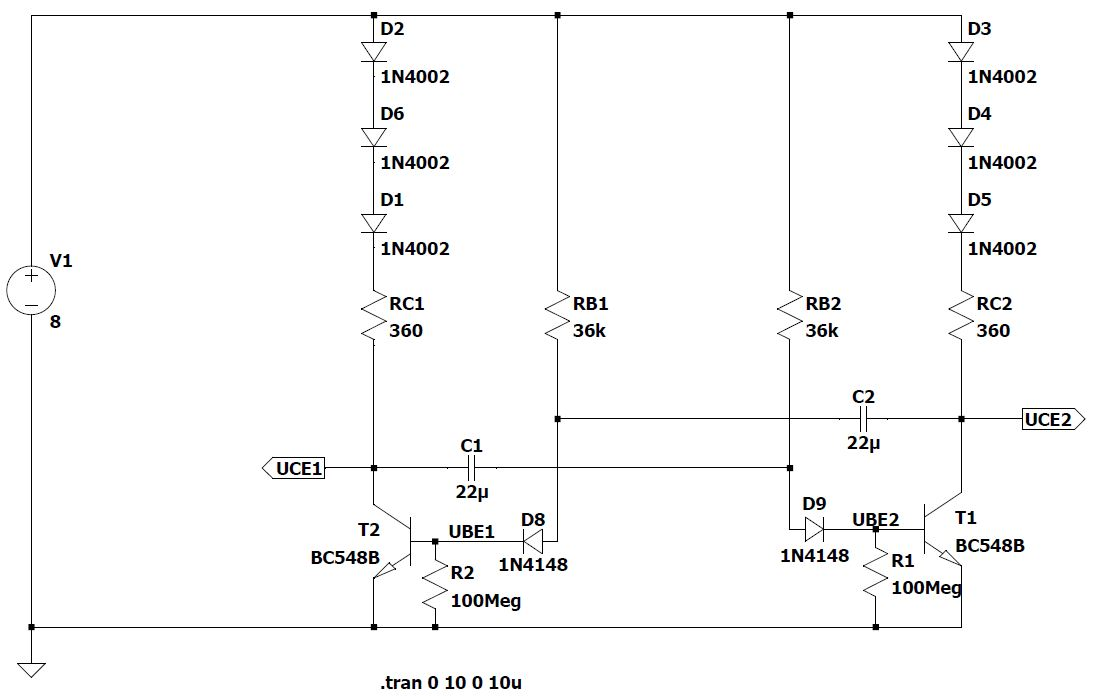
\includegraphics[width = 0.8\textwidth]{\figpath/Kipp_Schem_Diode.jpg}
    \caption{Astabile Kippschaltung in LTSpice mit Schutzdioden}
    \label{fig_Kap3_08:LTSpice_Schem_2}
\end{figure}

Die Basis-Emitter-Stufe ist sehr hochohmig, weswegen in der Simulation der Potentialbezug zur Masse verloren geht, wenn die Diode sperrt. Daher wurde auf beiden Seiten ein $\SI{100}{\mega\ohm}$ Widerstand eingefügt. Die Schaltung wurde 5 Sekunden lang mit Zeitschritten von $\SI{10}{\micro\second}$ simuliert. Die Spannungskurven können Abbildung \ref{fig_Kap3_09:Spannungen} entnommen werden.

\begin{figure}[H]
	\centering \small
	\scalebox{0.9}{% This file was created by matlab2tikz.
%
\definecolor{mycolor1}{rgb}{0.00000,0.44700,0.74100}%
\definecolor{mycolor2}{rgb}{0.85000,0.32500,0.09800}%
\definecolor{mycolor3}{rgb}{0.92900,0.69400,0.12500}%
\definecolor{mycolor4}{rgb}{0.49400,0.18400,0.55600}%
%
\begin{tikzpicture}

\begin{axis}[%
width=4.521in,
height=3.555in,
at={(0.758in,0.481in)},
scale only axis,
xmin=0,
xmax=5,
xlabel style={font=\color{white!15!black}},
xlabel={$t \text{ in s}$},
ymin=-1,
ymax=8,
ylabel style={font=\color{white!15!black}},
ylabel={$U \text{ in V}$},
axis background/.style={fill=white},
title style={font=\bfseries},
title={$U_{BE}$},
xmajorgrids,
ymajorgrids,
legend style={legend cell align=left, align=left, draw=white!15!black}
]
\addplot [color=mycolor1]
  table[row sep=crcr]{%
0	0.741\\
0.01	0.741\\
0.02	0.741\\
0.03	0.741\\
0.04	0.741\\
0.05	0.741\\
0.06	0.741\\
0.07	0.741\\
0.08	0.741\\
0.09	0.465\\
0.1	0.285\\
0.11	0.383\\
0.12	0.464\\
0.13	0.52\\
0.14	0.566\\
0.15	0.61\\
0.16	0.757\\
0.17	0.748\\
0.18	0.744\\
0.19	0.743\\
0.2	0.742\\
0.21	0.742\\
0.22	0.742\\
0.23	0.742\\
0.24	0.742\\
0.25	0.742\\
0.26	0.742\\
0.27	0.742\\
0.28	0.741\\
0.29	0.741\\
0.3	0.741\\
0.31	0.741\\
0.32	0.741\\
0.33	0.741\\
0.34	0.741\\
0.35	0.741\\
0.36	0.741\\
0.37	0.741\\
0.38	0.741\\
0.39	0.741\\
0.4	0.741\\
0.41	0.741\\
0.42	0.741\\
0.43	0.741\\
0.44	0.741\\
0.45	0.741\\
0.46	0.741\\
0.47	0.741\\
0.48	0.741\\
0.49	0.741\\
0.5	0.741\\
0.51	0.741\\
0.52	0.741\\
0.53	0.741\\
0.54	0.741\\
0.55	0.741\\
0.56	0.741\\
0.57	0.741\\
0.58	0.741\\
0.59	0.741\\
0.6	0.741\\
0.61	0.741\\
0.62	0.741\\
0.63	-0.109\\
0.64	-0.218\\
0.65	-0.237\\
0.66	-0.243\\
0.67	-0.245\\
0.68	-0.246\\
0.69	-0.247\\
0.7	-0.247\\
0.71	-0.247\\
0.72	-0.248\\
0.73	-0.248\\
0.74	-0.248\\
0.75	-0.248\\
0.76	-0.248\\
0.77	-0.248\\
0.78	-0.248\\
0.79	-0.248\\
0.8	-0.248\\
0.81	-0.248\\
0.82	-0.248\\
0.83	-0.248\\
0.84	-0.248\\
0.85	-0.248\\
0.86	-0.248\\
0.87	-0.248\\
0.88	-0.248\\
0.89	-0.248\\
0.9	-0.248\\
0.91	-0.248\\
0.92	-0.248\\
0.93	-0.248\\
0.94	-0.248\\
0.95	-0.248\\
0.96	-0.248\\
0.97	-0.247\\
0.98	-0.247\\
0.99	-0.247\\
1	-0.245\\
1.01	-0.232\\
1.02	-0.187\\
1.03	-0.116\\
1.04	-0.034\\
1.05	0.052\\
1.06	0.14\\
1.07	0.229\\
1.08	0.317\\
1.09	0.4\\
1.1	0.467\\
1.11	0.517\\
1.12	0.561\\
1.13	0.765\\
1.14	0.751\\
1.15	0.746\\
1.16	0.743\\
1.17	0.743\\
1.18	0.742\\
1.19	0.742\\
1.2	0.742\\
1.21	0.742\\
1.22	0.742\\
1.23	0.742\\
1.24	0.742\\
1.25	0.742\\
1.26	0.741\\
1.27	0.741\\
1.28	0.741\\
1.29	0.741\\
1.3	0.741\\
1.31	0.741\\
1.32	0.741\\
1.33	0.741\\
1.34	0.741\\
1.35	0.741\\
1.36	0.741\\
1.37	0.741\\
1.38	0.741\\
1.39	0.741\\
1.4	0.741\\
1.41	0.741\\
1.42	0.741\\
1.43	0.741\\
1.44	0.741\\
1.45	0.741\\
1.46	0.741\\
1.47	0.741\\
1.48	0.741\\
1.49	0.741\\
1.5	0.741\\
1.51	0.741\\
1.52	0.741\\
1.53	0.741\\
1.54	0.741\\
1.55	0.741\\
1.56	0.741\\
1.57	0.741\\
1.58	0.741\\
1.59	0.741\\
1.6	0.741\\
1.61	0.741\\
1.62	0.741\\
1.63	0.741\\
1.64	-0.156\\
1.65	-0.224\\
1.66	-0.239\\
1.67	-0.244\\
1.68	-0.246\\
1.69	-0.247\\
1.7	-0.247\\
1.71	-0.247\\
1.72	-0.248\\
1.73	-0.248\\
1.74	-0.248\\
1.75	-0.248\\
1.76	-0.248\\
1.77	-0.248\\
1.78	-0.248\\
1.79	-0.248\\
1.8	-0.248\\
1.81	-0.248\\
1.82	-0.248\\
1.83	-0.248\\
1.84	-0.248\\
1.85	-0.248\\
1.86	-0.248\\
1.87	-0.248\\
1.88	-0.248\\
1.89	-0.248\\
1.9	-0.248\\
1.91	-0.248\\
1.92	-0.248\\
1.93	-0.248\\
1.94	-0.248\\
1.95	-0.248\\
1.96	-0.248\\
1.97	-0.248\\
1.98	-0.247\\
1.99	-0.247\\
2	-0.247\\
2.01	-0.245\\
2.02	-0.229\\
2.03	-0.179\\
2.04	-0.107\\
2.05	-0.024\\
2.06	0.062\\
2.07	0.15\\
2.08	0.239\\
2.09	0.328\\
2.1	0.409\\
2.11	0.473\\
2.12	0.523\\
2.13	0.566\\
2.14	0.763\\
2.15	0.75\\
2.16	0.745\\
2.17	0.743\\
2.18	0.743\\
2.19	0.742\\
2.2	0.742\\
2.21	0.742\\
2.22	0.742\\
2.23	0.742\\
2.24	0.742\\
2.25	0.742\\
2.26	0.742\\
2.27	0.741\\
2.28	0.741\\
2.29	0.741\\
2.3	0.741\\
2.31	0.741\\
2.32	0.741\\
2.33	0.741\\
2.34	0.741\\
2.35	0.741\\
2.36	0.741\\
2.37	0.741\\
2.38	0.741\\
2.39	0.741\\
2.4	0.741\\
2.41	0.741\\
2.42	0.741\\
2.43	0.741\\
2.44	0.741\\
2.45	0.741\\
2.46	0.741\\
2.47	0.741\\
2.48	0.741\\
2.49	0.741\\
2.5	0.741\\
2.51	0.741\\
2.52	0.741\\
2.53	0.741\\
2.54	0.741\\
2.55	0.741\\
2.56	0.741\\
2.57	0.741\\
2.58	0.741\\
2.59	0.741\\
2.6	0.741\\
2.61	0.741\\
2.62	0.741\\
2.63	0.741\\
2.64	0.741\\
2.65	-0.173\\
2.66	-0.227\\
2.67	-0.24\\
2.68	-0.244\\
2.69	-0.246\\
2.7	-0.247\\
2.71	-0.247\\
2.72	-0.247\\
2.73	-0.248\\
2.74	-0.248\\
2.75	-0.248\\
2.76	-0.248\\
2.77	-0.248\\
2.78	-0.248\\
2.79	-0.248\\
2.8	-0.248\\
2.81	-0.248\\
2.82	-0.248\\
2.83	-0.248\\
2.84	-0.248\\
2.85	-0.248\\
2.86	-0.248\\
2.87	-0.248\\
2.88	-0.248\\
2.89	-0.248\\
2.9	-0.248\\
2.91	-0.248\\
2.92	-0.248\\
2.93	-0.248\\
2.94	-0.248\\
2.95	-0.248\\
2.96	-0.248\\
2.97	-0.248\\
2.98	-0.248\\
2.99	-0.247\\
3	-0.247\\
3.01	-0.247\\
3.02	-0.244\\
3.03	-0.225\\
3.04	-0.171\\
3.05	-0.097\\
3.06	-0.014\\
3.07	0.072\\
3.08	0.161\\
3.09	0.25\\
3.1	0.338\\
3.11	0.418\\
3.12	0.48\\
3.13	0.528\\
3.14	0.571\\
3.15	0.761\\
3.16	0.749\\
3.17	0.745\\
3.18	0.743\\
3.19	0.742\\
3.2	0.742\\
3.21	0.742\\
3.22	0.742\\
3.23	0.742\\
3.24	0.742\\
3.25	0.742\\
3.26	0.742\\
3.27	0.742\\
3.28	0.741\\
3.29	0.741\\
3.3	0.741\\
3.31	0.741\\
3.32	0.741\\
3.33	0.741\\
3.34	0.741\\
3.35	0.741\\
3.36	0.741\\
3.37	0.741\\
3.38	0.741\\
3.39	0.741\\
3.4	0.741\\
3.41	0.741\\
3.42	0.741\\
3.43	0.741\\
3.44	0.741\\
3.45	0.741\\
3.46	0.741\\
3.47	0.741\\
3.48	0.741\\
3.49	0.741\\
3.5	0.741\\
3.51	0.741\\
3.52	0.741\\
3.53	0.741\\
3.54	0.741\\
3.55	0.741\\
3.56	0.741\\
3.57	0.741\\
3.58	0.741\\
3.59	0.741\\
3.6	0.741\\
3.61	0.741\\
3.62	0.741\\
3.63	0.741\\
3.64	0.741\\
3.65	0.501\\
3.66	-0.186\\
3.67	-0.229\\
3.68	-0.241\\
3.69	-0.244\\
3.7	-0.246\\
3.71	-0.247\\
3.72	-0.247\\
3.73	-0.247\\
3.74	-0.248\\
3.75	-0.248\\
3.76	-0.248\\
3.77	-0.248\\
3.78	-0.248\\
3.79	-0.248\\
3.8	-0.248\\
3.81	-0.248\\
3.82	-0.248\\
3.83	-0.248\\
3.84	-0.248\\
3.85	-0.248\\
3.86	-0.248\\
3.87	-0.248\\
3.88	-0.248\\
3.89	-0.248\\
3.9	-0.248\\
3.91	-0.248\\
3.92	-0.248\\
3.93	-0.248\\
3.94	-0.248\\
3.95	-0.248\\
3.96	-0.248\\
3.97	-0.248\\
3.98	-0.248\\
3.99	-0.247\\
4	-0.247\\
4.01	-0.247\\
4.02	-0.247\\
4.03	-0.243\\
4.04	-0.22\\
4.05	-0.164\\
4.06	-0.088\\
4.07	-0.004\\
4.08	0.083\\
4.09	0.171\\
4.1	0.26\\
4.11	0.348\\
4.12	0.426\\
4.13	0.486\\
4.14	0.533\\
4.15	0.577\\
4.16	0.759\\
4.17	0.749\\
4.18	0.745\\
4.19	0.743\\
4.2	0.742\\
4.21	0.742\\
4.22	0.742\\
4.23	0.742\\
4.24	0.742\\
4.25	0.742\\
4.26	0.742\\
4.27	0.742\\
4.28	0.742\\
4.29	0.741\\
4.3	0.741\\
4.31	0.741\\
4.32	0.741\\
4.33	0.741\\
4.34	0.741\\
4.35	0.741\\
4.36	0.741\\
4.37	0.741\\
4.38	0.741\\
4.39	0.741\\
4.4	0.741\\
4.41	0.741\\
4.42	0.741\\
4.43	0.741\\
4.44	0.741\\
4.45	0.741\\
4.46	0.741\\
4.47	0.741\\
4.48	0.741\\
4.49	0.741\\
4.5	0.741\\
4.51	0.741\\
4.52	0.741\\
4.53	0.741\\
4.54	0.741\\
4.55	0.741\\
4.56	0.741\\
4.57	0.741\\
4.58	0.741\\
4.59	0.741\\
4.6	0.741\\
4.61	0.741\\
4.62	0.741\\
4.63	0.741\\
4.64	0.741\\
4.65	0.741\\
4.66	0.285\\
4.67	-0.195\\
4.68	-0.232\\
4.69	-0.241\\
4.7	-0.245\\
4.71	-0.246\\
4.72	-0.247\\
4.73	-0.247\\
4.74	-0.247\\
4.75	-0.248\\
4.76	-0.248\\
4.77	-0.248\\
4.78	-0.248\\
4.79	-0.248\\
4.8	-0.248\\
4.81	-0.248\\
4.82	-0.248\\
4.83	-0.248\\
4.84	-0.248\\
4.85	-0.248\\
4.86	-0.248\\
4.87	-0.248\\
4.88	-0.248\\
4.89	-0.248\\
4.9	-0.248\\
4.91	-0.248\\
4.92	-0.248\\
4.93	-0.248\\
4.94	-0.248\\
4.95	-0.248\\
4.96	-0.248\\
4.97	-0.248\\
4.98	-0.248\\
4.99	-0.248\\
5	-0.248\\
};
\addlegendentry{$\text{U}_{\text{BE1}}$}

\addplot [color=mycolor2]
  table[row sep=crcr]{%
0	0.741\\
0.01	0.741\\
0.02	0.741\\
0.03	0.741\\
0.04	0.741\\
0.05	0.741\\
0.06	0.741\\
0.07	0.741\\
0.08	0.741\\
0.09	0.771\\
0.1	0.754\\
0.11	0.746\\
0.12	0.744\\
0.13	0.742\\
0.14	0.742\\
0.15	0.741\\
0.16	-0.146\\
0.17	-0.222\\
0.18	-0.239\\
0.19	-0.244\\
0.2	-0.246\\
0.21	-0.247\\
0.22	-0.247\\
0.23	-0.247\\
0.24	-0.247\\
0.25	-0.248\\
0.26	-0.248\\
0.27	-0.248\\
0.28	-0.248\\
0.29	-0.248\\
0.3	-0.248\\
0.31	-0.248\\
0.32	-0.248\\
0.33	-0.248\\
0.34	-0.248\\
0.35	-0.248\\
0.36	-0.248\\
0.37	-0.248\\
0.38	-0.248\\
0.39	-0.248\\
0.4	-0.248\\
0.41	-0.248\\
0.42	-0.248\\
0.43	-0.248\\
0.44	-0.248\\
0.45	-0.248\\
0.46	-0.247\\
0.47	-0.247\\
0.48	-0.247\\
0.49	-0.247\\
0.5	-0.243\\
0.51	-0.219\\
0.52	-0.162\\
0.53	-0.086\\
0.54	-0.003\\
0.55	0.085\\
0.56	0.173\\
0.57	0.262\\
0.58	0.349\\
0.59	0.428\\
0.6	0.487\\
0.61	0.534\\
0.62	0.578\\
0.63	0.759\\
0.64	0.749\\
0.65	0.745\\
0.66	0.743\\
0.67	0.742\\
0.68	0.742\\
0.69	0.742\\
0.7	0.742\\
0.71	0.742\\
0.72	0.742\\
0.73	0.742\\
0.74	0.742\\
0.75	0.741\\
0.76	0.741\\
0.77	0.741\\
0.78	0.741\\
0.79	0.741\\
0.8	0.741\\
0.81	0.741\\
0.82	0.741\\
0.83	0.741\\
0.84	0.741\\
0.85	0.741\\
0.86	0.741\\
0.87	0.741\\
0.88	0.741\\
0.89	0.741\\
0.9	0.741\\
0.91	0.741\\
0.92	0.741\\
0.93	0.741\\
0.94	0.741\\
0.95	0.741\\
0.96	0.741\\
0.97	0.741\\
0.98	0.741\\
0.99	0.741\\
1	0.741\\
1.01	0.741\\
1.02	0.741\\
1.03	0.741\\
1.04	0.741\\
1.05	0.741\\
1.06	0.741\\
1.07	0.741\\
1.08	0.741\\
1.09	0.741\\
1.1	0.741\\
1.11	0.741\\
1.12	0.741\\
1.13	0.17\\
1.14	-0.201\\
1.15	-0.233\\
1.16	-0.242\\
1.17	-0.245\\
1.18	-0.246\\
1.19	-0.247\\
1.2	-0.247\\
1.21	-0.247\\
1.22	-0.248\\
1.23	-0.248\\
1.24	-0.248\\
1.25	-0.248\\
1.26	-0.248\\
1.27	-0.248\\
1.28	-0.248\\
1.29	-0.248\\
1.3	-0.248\\
1.31	-0.248\\
1.32	-0.248\\
1.33	-0.248\\
1.34	-0.248\\
1.35	-0.248\\
1.36	-0.248\\
1.37	-0.248\\
1.38	-0.248\\
1.39	-0.248\\
1.4	-0.248\\
1.41	-0.248\\
1.42	-0.248\\
1.43	-0.248\\
1.44	-0.248\\
1.45	-0.248\\
1.46	-0.248\\
1.47	-0.248\\
1.48	-0.247\\
1.49	-0.247\\
1.5	-0.246\\
1.51	-0.241\\
1.52	-0.211\\
1.53	-0.149\\
1.54	-0.071\\
1.55	0.013\\
1.56	0.101\\
1.57	0.19\\
1.58	0.279\\
1.59	0.365\\
1.6	0.44\\
1.61	0.497\\
1.62	0.542\\
1.63	0.586\\
1.64	0.756\\
1.65	0.747\\
1.66	0.744\\
1.67	0.743\\
1.68	0.742\\
1.69	0.742\\
1.7	0.742\\
1.71	0.742\\
1.72	0.742\\
1.73	0.742\\
1.74	0.742\\
1.75	0.742\\
1.76	0.741\\
1.77	0.741\\
1.78	0.741\\
1.79	0.741\\
1.8	0.741\\
1.81	0.741\\
1.82	0.741\\
1.83	0.741\\
1.84	0.741\\
1.85	0.741\\
1.86	0.741\\
1.87	0.741\\
1.88	0.741\\
1.89	0.741\\
1.9	0.741\\
1.91	0.741\\
1.92	0.741\\
1.93	0.741\\
1.94	0.741\\
1.95	0.741\\
1.96	0.741\\
1.97	0.741\\
1.98	0.741\\
1.99	0.741\\
2	0.741\\
2.01	0.741\\
2.02	0.741\\
2.03	0.741\\
2.04	0.741\\
2.05	0.741\\
2.06	0.741\\
2.07	0.741\\
2.08	0.741\\
2.09	0.741\\
2.1	0.741\\
2.11	0.741\\
2.12	0.741\\
2.13	0.741\\
2.14	0.039\\
2.15	-0.208\\
2.16	-0.235\\
2.17	-0.242\\
2.18	-0.245\\
2.19	-0.246\\
2.2	-0.247\\
2.21	-0.247\\
2.22	-0.247\\
2.23	-0.248\\
2.24	-0.248\\
2.25	-0.248\\
2.26	-0.248\\
2.27	-0.248\\
2.28	-0.248\\
2.29	-0.248\\
2.3	-0.248\\
2.31	-0.248\\
2.32	-0.248\\
2.33	-0.248\\
2.34	-0.248\\
2.35	-0.248\\
2.36	-0.248\\
2.37	-0.248\\
2.38	-0.248\\
2.39	-0.248\\
2.4	-0.248\\
2.41	-0.248\\
2.42	-0.248\\
2.43	-0.248\\
2.44	-0.248\\
2.45	-0.248\\
2.46	-0.248\\
2.47	-0.248\\
2.48	-0.247\\
2.49	-0.247\\
2.5	-0.247\\
2.51	-0.246\\
2.52	-0.239\\
2.53	-0.205\\
2.54	-0.14\\
2.55	-0.061\\
2.56	0.024\\
2.57	0.111\\
2.58	0.2\\
2.59	0.289\\
2.6	0.375\\
2.61	0.447\\
2.62	0.502\\
2.63	0.547\\
2.64	0.593\\
2.65	0.755\\
2.66	0.747\\
2.67	0.744\\
2.68	0.743\\
2.69	0.742\\
2.7	0.742\\
2.71	0.742\\
2.72	0.742\\
2.73	0.742\\
2.74	0.742\\
2.75	0.742\\
2.76	0.742\\
2.77	0.741\\
2.78	0.741\\
2.79	0.741\\
2.8	0.741\\
2.81	0.741\\
2.82	0.741\\
2.83	0.741\\
2.84	0.741\\
2.85	0.741\\
2.86	0.741\\
2.87	0.741\\
2.88	0.741\\
2.89	0.741\\
2.9	0.741\\
2.91	0.741\\
2.92	0.741\\
2.93	0.741\\
2.94	0.741\\
2.95	0.741\\
2.96	0.741\\
2.97	0.741\\
2.98	0.741\\
2.99	0.741\\
3	0.741\\
3.01	0.741\\
3.02	0.741\\
3.03	0.741\\
3.04	0.741\\
3.05	0.741\\
3.06	0.741\\
3.07	0.741\\
3.08	0.741\\
3.09	0.741\\
3.1	0.741\\
3.11	0.741\\
3.12	0.741\\
3.13	0.741\\
3.14	0.741\\
3.15	-0.048\\
3.16	-0.213\\
3.17	-0.236\\
3.18	-0.243\\
3.19	-0.245\\
3.2	-0.246\\
3.21	-0.247\\
3.22	-0.247\\
3.23	-0.247\\
3.24	-0.248\\
3.25	-0.248\\
3.26	-0.248\\
3.27	-0.248\\
3.28	-0.248\\
3.29	-0.248\\
3.3	-0.248\\
3.31	-0.248\\
3.32	-0.248\\
3.33	-0.248\\
3.34	-0.248\\
3.35	-0.248\\
3.36	-0.248\\
3.37	-0.248\\
3.38	-0.248\\
3.39	-0.248\\
3.4	-0.248\\
3.41	-0.248\\
3.42	-0.248\\
3.43	-0.248\\
3.44	-0.248\\
3.45	-0.248\\
3.46	-0.248\\
3.47	-0.248\\
3.48	-0.248\\
3.49	-0.248\\
3.5	-0.247\\
3.51	-0.247\\
3.52	-0.246\\
3.53	-0.237\\
3.54	-0.199\\
3.55	-0.132\\
3.56	-0.052\\
3.57	0.034\\
3.58	0.122\\
3.59	0.211\\
3.6	0.299\\
3.61	0.384\\
3.62	0.455\\
3.63	0.508\\
3.64	0.552\\
3.65	0.77\\
3.66	0.753\\
3.67	0.746\\
3.68	0.744\\
3.69	0.743\\
3.7	0.742\\
3.71	0.742\\
3.72	0.742\\
3.73	0.742\\
3.74	0.742\\
3.75	0.742\\
3.76	0.742\\
3.77	0.742\\
3.78	0.741\\
3.79	0.741\\
3.8	0.741\\
3.81	0.741\\
3.82	0.741\\
3.83	0.741\\
3.84	0.741\\
3.85	0.741\\
3.86	0.741\\
3.87	0.741\\
3.88	0.741\\
3.89	0.741\\
3.9	0.741\\
3.91	0.741\\
3.92	0.741\\
3.93	0.741\\
3.94	0.741\\
3.95	0.741\\
3.96	0.741\\
3.97	0.741\\
3.98	0.741\\
3.99	0.741\\
4	0.741\\
4.01	0.741\\
4.02	0.741\\
4.03	0.741\\
4.04	0.741\\
4.05	0.741\\
4.06	0.741\\
4.07	0.741\\
4.08	0.741\\
4.09	0.741\\
4.1	0.741\\
4.11	0.741\\
4.12	0.741\\
4.13	0.741\\
4.14	0.741\\
4.15	0.741\\
4.16	-0.103\\
4.17	-0.218\\
4.18	-0.237\\
4.19	-0.243\\
4.2	-0.245\\
4.21	-0.246\\
4.22	-0.247\\
4.23	-0.247\\
4.24	-0.248\\
4.25	-0.248\\
4.26	-0.248\\
4.27	-0.248\\
4.28	-0.248\\
4.29	-0.248\\
4.3	-0.248\\
4.31	-0.248\\
4.32	-0.248\\
4.33	-0.248\\
4.34	-0.248\\
4.35	-0.248\\
4.36	-0.248\\
4.37	-0.248\\
4.38	-0.248\\
4.39	-0.248\\
4.4	-0.248\\
4.41	-0.248\\
4.42	-0.248\\
4.43	-0.248\\
4.44	-0.248\\
4.45	-0.248\\
4.46	-0.248\\
4.47	-0.248\\
4.48	-0.248\\
4.49	-0.248\\
4.5	-0.247\\
4.51	-0.247\\
4.52	-0.247\\
4.53	-0.246\\
4.54	-0.234\\
4.55	-0.192\\
4.56	-0.123\\
4.57	-0.042\\
4.58	0.044\\
4.59	0.132\\
4.6	0.221\\
4.61	0.309\\
4.62	0.393\\
4.63	0.462\\
4.64	0.513\\
4.65	0.557\\
4.66	0.767\\
4.67	0.752\\
4.68	0.746\\
4.69	0.744\\
4.7	0.743\\
4.71	0.742\\
4.72	0.742\\
4.73	0.742\\
4.74	0.742\\
4.75	0.742\\
4.76	0.742\\
4.77	0.742\\
4.78	0.742\\
4.79	0.741\\
4.8	0.741\\
4.81	0.741\\
4.82	0.741\\
4.83	0.741\\
4.84	0.741\\
4.85	0.741\\
4.86	0.741\\
4.87	0.741\\
4.88	0.741\\
4.89	0.741\\
4.9	0.741\\
4.91	0.741\\
4.92	0.741\\
4.93	0.741\\
4.94	0.741\\
4.95	0.741\\
4.96	0.741\\
4.97	0.741\\
4.98	0.741\\
4.99	0.741\\
5	0.741\\
};
\addlegendentry{$\text{U}_{\text{BE2}}$}

\addplot [color=mycolor3]
  table[row sep=crcr]{%
0	0.145\\
0.01	0.145\\
0.02	0.145\\
0.03	0.145\\
0.04	0.145\\
0.05	0.145\\
0.06	0.145\\
0.07	0.145\\
0.08	0.145\\
0.09	0.507\\
0.1	4.391\\
0.11	5.618\\
0.12	6.078\\
0.13	6.292\\
0.14	6.409\\
0.15	6.456\\
0.16	0.062\\
0.17	0.08\\
0.18	0.097\\
0.19	0.11\\
0.2	0.118\\
0.21	0.124\\
0.22	0.128\\
0.23	0.131\\
0.24	0.133\\
0.25	0.135\\
0.26	0.136\\
0.27	0.137\\
0.28	0.138\\
0.29	0.139\\
0.3	0.139\\
0.31	0.14\\
0.32	0.14\\
0.33	0.141\\
0.34	0.141\\
0.35	0.141\\
0.36	0.142\\
0.37	0.142\\
0.38	0.142\\
0.39	0.142\\
0.4	0.142\\
0.41	0.142\\
0.42	0.143\\
0.43	0.143\\
0.44	0.143\\
0.45	0.143\\
0.46	0.143\\
0.47	0.143\\
0.48	0.143\\
0.49	0.143\\
0.5	0.143\\
0.51	0.143\\
0.52	0.143\\
0.53	0.143\\
0.54	0.143\\
0.55	0.144\\
0.56	0.144\\
0.57	0.144\\
0.58	0.144\\
0.59	0.144\\
0.6	0.144\\
0.61	0.145\\
0.62	0.152\\
0.63	3.434\\
0.64	5.3\\
0.65	5.95\\
0.66	6.228\\
0.67	6.376\\
0.68	6.47\\
0.69	6.537\\
0.7	6.587\\
0.71	6.627\\
0.72	6.661\\
0.73	6.689\\
0.74	6.713\\
0.75	6.735\\
0.76	6.754\\
0.77	6.771\\
0.78	6.787\\
0.79	6.801\\
0.8	6.815\\
0.81	6.827\\
0.82	6.838\\
0.83	6.849\\
0.84	6.859\\
0.85	6.869\\
0.86	6.878\\
0.87	6.886\\
0.88	6.894\\
0.89	6.902\\
0.9	6.909\\
0.91	6.917\\
0.92	6.923\\
0.93	6.93\\
0.94	6.936\\
0.95	6.942\\
0.96	6.948\\
0.97	6.953\\
0.98	6.959\\
0.99	6.964\\
1	6.969\\
1.01	6.974\\
1.02	6.979\\
1.03	6.983\\
1.04	6.988\\
1.05	6.992\\
1.06	6.996\\
1.07	7.001\\
1.08	7.005\\
1.09	7.009\\
1.1	7.012\\
1.11	7.015\\
1.12	7.01\\
1.13	0.055\\
1.14	0.07\\
1.15	0.089\\
1.16	0.104\\
1.17	0.114\\
1.18	0.122\\
1.19	0.126\\
1.2	0.13\\
1.21	0.132\\
1.22	0.134\\
1.23	0.136\\
1.24	0.137\\
1.25	0.138\\
1.26	0.139\\
1.27	0.139\\
1.28	0.14\\
1.29	0.14\\
1.3	0.141\\
1.31	0.141\\
1.32	0.141\\
1.33	0.141\\
1.34	0.142\\
1.35	0.142\\
1.36	0.142\\
1.37	0.142\\
1.38	0.142\\
1.39	0.143\\
1.4	0.143\\
1.41	0.143\\
1.42	0.143\\
1.43	0.143\\
1.44	0.143\\
1.45	0.143\\
1.46	0.143\\
1.47	0.143\\
1.48	0.143\\
1.49	0.143\\
1.5	0.143\\
1.51	0.143\\
1.52	0.144\\
1.53	0.144\\
1.54	0.144\\
1.55	0.144\\
1.56	0.144\\
1.57	0.144\\
1.58	0.144\\
1.59	0.144\\
1.6	0.144\\
1.61	0.144\\
1.62	0.146\\
1.63	0.156\\
1.64	3.973\\
1.65	5.479\\
1.66	6.02\\
1.67	6.262\\
1.68	6.397\\
1.69	6.484\\
1.7	6.547\\
1.71	6.595\\
1.72	6.634\\
1.73	6.666\\
1.74	6.694\\
1.75	6.718\\
1.76	6.739\\
1.77	6.757\\
1.78	6.774\\
1.79	6.79\\
1.8	6.804\\
1.81	6.817\\
1.82	6.829\\
1.83	6.841\\
1.84	6.851\\
1.85	6.861\\
1.86	6.871\\
1.87	6.879\\
1.88	6.888\\
1.89	6.896\\
1.9	6.904\\
1.91	6.911\\
1.92	6.918\\
1.93	6.925\\
1.94	6.931\\
1.95	6.937\\
1.96	6.943\\
1.97	6.949\\
1.98	6.954\\
1.99	6.96\\
2	6.965\\
2.01	6.97\\
2.02	6.975\\
2.03	6.98\\
2.04	6.984\\
2.05	6.989\\
2.06	6.993\\
2.07	6.997\\
2.08	7.002\\
2.09	7.005\\
2.1	7.009\\
2.11	7.013\\
2.12	7.015\\
2.13	7.008\\
2.14	0.057\\
2.15	0.072\\
2.16	0.091\\
2.17	0.105\\
2.18	0.115\\
2.19	0.122\\
2.2	0.127\\
2.21	0.13\\
2.22	0.133\\
2.23	0.134\\
2.24	0.136\\
2.25	0.137\\
2.26	0.138\\
2.27	0.139\\
2.28	0.139\\
2.29	0.14\\
2.3	0.14\\
2.31	0.141\\
2.32	0.141\\
2.33	0.141\\
2.34	0.141\\
2.35	0.142\\
2.36	0.142\\
2.37	0.142\\
2.38	0.142\\
2.39	0.142\\
2.4	0.143\\
2.41	0.143\\
2.42	0.143\\
2.43	0.143\\
2.44	0.143\\
2.45	0.143\\
2.46	0.143\\
2.47	0.143\\
2.48	0.143\\
2.49	0.143\\
2.5	0.143\\
2.51	0.143\\
2.52	0.143\\
2.53	0.144\\
2.54	0.144\\
2.55	0.144\\
2.56	0.144\\
2.57	0.144\\
2.58	0.144\\
2.59	0.144\\
2.6	0.144\\
2.61	0.144\\
2.62	0.144\\
2.63	0.146\\
2.64	0.16\\
2.65	4.248\\
2.66	5.57\\
2.67	6.057\\
2.68	6.282\\
2.69	6.409\\
2.7	6.493\\
2.71	6.554\\
2.72	6.6\\
2.73	6.638\\
2.74	6.67\\
2.75	6.697\\
2.76	6.72\\
2.77	6.741\\
2.78	6.759\\
2.79	6.776\\
2.8	6.792\\
2.81	6.806\\
2.82	6.819\\
2.83	6.831\\
2.84	6.842\\
2.85	6.852\\
2.86	6.862\\
2.87	6.872\\
2.88	6.88\\
2.89	6.889\\
2.9	6.897\\
2.91	6.904\\
2.92	6.912\\
2.93	6.919\\
2.94	6.925\\
2.95	6.932\\
2.96	6.938\\
2.97	6.944\\
2.98	6.95\\
2.99	6.955\\
3	6.96\\
3.01	6.966\\
3.02	6.971\\
3.03	6.976\\
3.04	6.98\\
3.05	6.985\\
3.06	6.989\\
3.07	6.994\\
3.08	6.998\\
3.09	7.002\\
3.1	7.006\\
3.11	7.01\\
3.12	7.013\\
3.13	7.015\\
3.14	7.006\\
3.15	0.058\\
3.16	0.075\\
3.17	0.093\\
3.18	0.107\\
3.19	0.116\\
3.2	0.123\\
3.21	0.127\\
3.22	0.131\\
3.23	0.133\\
3.24	0.135\\
3.25	0.136\\
3.26	0.137\\
3.27	0.138\\
3.28	0.139\\
3.29	0.139\\
3.3	0.14\\
3.31	0.14\\
3.32	0.141\\
3.33	0.141\\
3.34	0.141\\
3.35	0.141\\
3.36	0.142\\
3.37	0.142\\
3.38	0.142\\
3.39	0.142\\
3.4	0.142\\
3.41	0.143\\
3.42	0.143\\
3.43	0.143\\
3.44	0.143\\
3.45	0.143\\
3.46	0.143\\
3.47	0.143\\
3.48	0.143\\
3.49	0.143\\
3.5	0.143\\
3.51	0.143\\
3.52	0.143\\
3.53	0.143\\
3.54	0.144\\
3.55	0.144\\
3.56	0.144\\
3.57	0.144\\
3.58	0.144\\
3.59	0.144\\
3.6	0.144\\
3.61	0.144\\
3.62	0.144\\
3.63	0.144\\
3.64	0.147\\
3.65	0.839\\
3.66	4.488\\
3.67	5.654\\
3.68	6.093\\
3.69	6.3\\
3.7	6.421\\
3.71	6.501\\
3.72	6.56\\
3.73	6.605\\
3.74	6.642\\
3.75	6.673\\
3.76	6.7\\
3.77	6.723\\
3.78	6.743\\
3.79	6.762\\
3.8	6.778\\
3.81	6.793\\
3.82	6.807\\
3.83	6.82\\
3.84	6.832\\
3.85	6.843\\
3.86	6.854\\
3.87	6.863\\
3.88	6.873\\
3.89	6.881\\
3.9	6.89\\
3.91	6.898\\
3.92	6.905\\
3.93	6.913\\
3.94	6.919\\
3.95	6.926\\
3.96	6.932\\
3.97	6.939\\
3.98	6.945\\
3.99	6.95\\
4	6.956\\
4.01	6.961\\
4.02	6.966\\
4.03	6.971\\
4.04	6.976\\
4.05	6.981\\
4.06	6.985\\
4.07	6.99\\
4.08	6.994\\
4.09	6.998\\
4.1	7.002\\
4.11	7.006\\
4.12	7.01\\
4.13	7.014\\
4.14	7.014\\
4.15	7.002\\
4.16	0.06\\
4.17	0.077\\
4.18	0.095\\
4.19	0.108\\
4.2	0.117\\
4.21	0.124\\
4.22	0.128\\
4.23	0.131\\
4.24	0.133\\
4.25	0.135\\
4.26	0.136\\
4.27	0.137\\
4.28	0.138\\
4.29	0.139\\
4.3	0.139\\
4.31	0.14\\
4.32	0.14\\
4.33	0.141\\
4.34	0.141\\
4.35	0.141\\
4.36	0.142\\
4.37	0.142\\
4.38	0.142\\
4.39	0.142\\
4.4	0.142\\
4.41	0.142\\
4.42	0.143\\
4.43	0.143\\
4.44	0.143\\
4.45	0.143\\
4.46	0.143\\
4.47	0.143\\
4.48	0.143\\
4.49	0.143\\
4.5	0.143\\
4.51	0.143\\
4.52	0.143\\
4.53	0.143\\
4.54	0.143\\
4.55	0.144\\
4.56	0.144\\
4.57	0.144\\
4.58	0.144\\
4.59	0.144\\
4.6	0.144\\
4.61	0.144\\
4.62	0.144\\
4.63	0.144\\
4.64	0.144\\
4.65	0.147\\
4.66	1.525\\
4.67	4.699\\
4.68	5.727\\
4.69	6.125\\
4.7	6.318\\
4.71	6.432\\
4.72	6.509\\
4.73	6.566\\
4.74	6.61\\
4.75	6.646\\
4.76	6.676\\
4.77	6.702\\
4.78	6.725\\
4.79	6.745\\
4.8	6.763\\
4.81	6.78\\
4.82	6.795\\
4.83	6.809\\
4.84	6.821\\
4.85	6.833\\
4.86	6.844\\
4.87	6.855\\
4.88	6.864\\
4.89	6.874\\
4.9	6.882\\
4.91	6.891\\
4.92	6.899\\
4.93	6.906\\
4.94	6.913\\
4.95	6.92\\
4.96	6.927\\
4.97	6.933\\
4.98	6.939\\
4.99	6.945\\
5	6.951\\
};
\addlegendentry{$\text{U}_{\text{CE1}}$}

\addplot [color=mycolor4]
  table[row sep=crcr]{%
0	0.145\\
0.01	0.145\\
0.02	0.145\\
0.03	0.145\\
0.04	0.145\\
0.05	0.145\\
0.06	0.145\\
0.07	0.145\\
0.08	0.145\\
0.09	0.053\\
0.1	0.065\\
0.11	0.084\\
0.12	0.1\\
0.13	0.112\\
0.14	0.121\\
0.15	0.135\\
0.16	3.828\\
0.17	5.429\\
0.18	6.001\\
0.19	6.253\\
0.2	6.391\\
0.21	6.481\\
0.22	6.544\\
0.23	6.593\\
0.24	6.632\\
0.25	6.665\\
0.26	6.692\\
0.27	6.716\\
0.28	6.737\\
0.29	6.756\\
0.3	6.773\\
0.31	6.789\\
0.32	6.803\\
0.33	6.816\\
0.34	6.829\\
0.35	6.84\\
0.36	6.851\\
0.37	6.861\\
0.38	6.87\\
0.39	6.879\\
0.4	6.887\\
0.41	6.895\\
0.42	6.903\\
0.43	6.91\\
0.44	6.917\\
0.45	6.924\\
0.46	6.931\\
0.47	6.937\\
0.48	6.943\\
0.49	6.949\\
0.5	6.954\\
0.51	6.96\\
0.52	6.965\\
0.53	6.97\\
0.54	6.975\\
0.55	6.979\\
0.56	6.984\\
0.57	6.988\\
0.58	6.993\\
0.59	6.997\\
0.6	7.001\\
0.61	7.002\\
0.62	6.989\\
0.63	0.06\\
0.64	0.077\\
0.65	0.095\\
0.66	0.108\\
0.67	0.117\\
0.68	0.124\\
0.69	0.128\\
0.7	0.131\\
0.71	0.133\\
0.72	0.135\\
0.73	0.136\\
0.74	0.137\\
0.75	0.138\\
0.76	0.139\\
0.77	0.139\\
0.78	0.14\\
0.79	0.14\\
0.8	0.141\\
0.81	0.141\\
0.82	0.141\\
0.83	0.142\\
0.84	0.142\\
0.85	0.142\\
0.86	0.142\\
0.87	0.142\\
0.88	0.142\\
0.89	0.143\\
0.9	0.143\\
0.91	0.143\\
0.92	0.143\\
0.93	0.143\\
0.94	0.143\\
0.95	0.143\\
0.96	0.143\\
0.97	0.143\\
0.98	0.143\\
0.99	0.143\\
1	0.143\\
1.01	0.143\\
1.02	0.144\\
1.03	0.144\\
1.04	0.144\\
1.05	0.144\\
1.06	0.144\\
1.07	0.144\\
1.08	0.144\\
1.09	0.144\\
1.1	0.144\\
1.11	0.145\\
1.12	0.148\\
1.13	1.981\\
1.14	4.838\\
1.15	5.779\\
1.16	6.147\\
1.17	6.33\\
1.18	6.44\\
1.19	6.514\\
1.2	6.57\\
1.21	6.613\\
1.22	6.649\\
1.23	6.679\\
1.24	6.705\\
1.25	6.727\\
1.26	6.747\\
1.27	6.765\\
1.28	6.781\\
1.29	6.796\\
1.3	6.81\\
1.31	6.823\\
1.32	6.834\\
1.33	6.845\\
1.34	6.856\\
1.35	6.865\\
1.36	6.874\\
1.37	6.883\\
1.38	6.891\\
1.39	6.899\\
1.4	6.907\\
1.41	6.914\\
1.42	6.921\\
1.43	6.927\\
1.44	6.934\\
1.45	6.94\\
1.46	6.946\\
1.47	6.951\\
1.48	6.957\\
1.49	6.962\\
1.5	6.967\\
1.51	6.972\\
1.52	6.977\\
1.53	6.982\\
1.54	6.986\\
1.55	6.991\\
1.56	6.995\\
1.57	6.999\\
1.58	7.003\\
1.59	7.007\\
1.6	7.011\\
1.61	7.014\\
1.62	7.014\\
1.63	6.994\\
1.64	0.063\\
1.65	0.081\\
1.66	0.098\\
1.67	0.11\\
1.68	0.119\\
1.69	0.125\\
1.7	0.129\\
1.71	0.131\\
1.72	0.134\\
1.73	0.135\\
1.74	0.136\\
1.75	0.137\\
1.76	0.138\\
1.77	0.139\\
1.78	0.139\\
1.79	0.14\\
1.8	0.14\\
1.81	0.141\\
1.82	0.141\\
1.83	0.141\\
1.84	0.142\\
1.85	0.142\\
1.86	0.142\\
1.87	0.142\\
1.88	0.142\\
1.89	0.142\\
1.9	0.143\\
1.91	0.143\\
1.92	0.143\\
1.93	0.143\\
1.94	0.143\\
1.95	0.143\\
1.96	0.143\\
1.97	0.143\\
1.98	0.143\\
1.99	0.143\\
2	0.143\\
2.01	0.143\\
2.02	0.143\\
2.03	0.144\\
2.04	0.144\\
2.05	0.144\\
2.06	0.144\\
2.07	0.144\\
2.08	0.144\\
2.09	0.144\\
2.1	0.144\\
2.11	0.144\\
2.12	0.145\\
2.13	0.149\\
2.14	2.52\\
2.15	5.008\\
2.16	5.838\\
2.17	6.175\\
2.18	6.346\\
2.19	6.45\\
2.2	6.522\\
2.21	6.576\\
2.22	6.618\\
2.23	6.653\\
2.24	6.682\\
2.25	6.707\\
2.26	6.73\\
2.27	6.749\\
2.28	6.767\\
2.29	6.783\\
2.3	6.798\\
2.31	6.811\\
2.32	6.824\\
2.33	6.836\\
2.34	6.847\\
2.35	6.857\\
2.36	6.866\\
2.37	6.876\\
2.38	6.884\\
2.39	6.892\\
2.4	6.9\\
2.41	6.908\\
2.42	6.915\\
2.43	6.922\\
2.44	6.928\\
2.45	6.934\\
2.46	6.941\\
2.47	6.946\\
2.48	6.952\\
2.49	6.957\\
2.5	6.963\\
2.51	6.968\\
2.52	6.973\\
2.53	6.978\\
2.54	6.982\\
2.55	6.987\\
2.56	6.991\\
2.57	6.996\\
2.58	7\\
2.59	7.004\\
2.6	7.008\\
2.61	7.011\\
2.62	7.014\\
2.63	7.013\\
2.64	6.986\\
2.65	0.065\\
2.66	0.083\\
2.67	0.099\\
2.68	0.111\\
2.69	0.12\\
2.7	0.125\\
2.71	0.129\\
2.72	0.132\\
2.73	0.134\\
2.74	0.135\\
2.75	0.137\\
2.76	0.138\\
2.77	0.138\\
2.78	0.139\\
2.79	0.14\\
2.8	0.14\\
2.81	0.14\\
2.82	0.141\\
2.83	0.141\\
2.84	0.141\\
2.85	0.142\\
2.86	0.142\\
2.87	0.142\\
2.88	0.142\\
2.89	0.142\\
2.9	0.142\\
2.91	0.143\\
2.92	0.143\\
2.93	0.143\\
2.94	0.143\\
2.95	0.143\\
2.96	0.143\\
2.97	0.143\\
2.98	0.143\\
2.99	0.143\\
3	0.143\\
3.01	0.143\\
3.02	0.143\\
3.03	0.143\\
3.04	0.144\\
3.05	0.144\\
3.06	0.144\\
3.07	0.144\\
3.08	0.144\\
3.09	0.144\\
3.1	0.144\\
3.11	0.144\\
3.12	0.144\\
3.13	0.145\\
3.14	0.15\\
3.15	2.983\\
3.16	5.156\\
3.17	5.894\\
3.18	6.201\\
3.19	6.361\\
3.2	6.46\\
3.21	6.529\\
3.22	6.581\\
3.23	6.622\\
3.24	6.656\\
3.25	6.685\\
3.26	6.71\\
3.27	6.732\\
3.28	6.752\\
3.29	6.769\\
3.3	6.785\\
3.31	6.8\\
3.32	6.813\\
3.33	6.825\\
3.34	6.837\\
3.35	6.848\\
3.36	6.858\\
3.37	6.868\\
3.38	6.877\\
3.39	6.885\\
3.4	6.893\\
3.41	6.901\\
3.42	6.909\\
3.43	6.916\\
3.44	6.922\\
3.45	6.929\\
3.46	6.935\\
3.47	6.941\\
3.48	6.947\\
3.49	6.953\\
3.5	6.958\\
3.51	6.963\\
3.52	6.968\\
3.53	6.973\\
3.54	6.978\\
3.55	6.983\\
3.56	6.987\\
3.57	6.992\\
3.58	6.996\\
3.59	7\\
3.6	7.004\\
3.61	7.008\\
3.62	7.012\\
3.63	7.015\\
3.64	7.012\\
3.65	0.053\\
3.66	0.067\\
3.67	0.085\\
3.68	0.101\\
3.69	0.113\\
3.7	0.12\\
3.71	0.126\\
3.72	0.129\\
3.73	0.132\\
3.74	0.134\\
3.75	0.135\\
3.76	0.137\\
3.77	0.138\\
3.78	0.138\\
3.79	0.139\\
3.8	0.14\\
3.81	0.14\\
3.82	0.14\\
3.83	0.141\\
3.84	0.141\\
3.85	0.141\\
3.86	0.142\\
3.87	0.142\\
3.88	0.142\\
3.89	0.142\\
3.9	0.142\\
3.91	0.142\\
3.92	0.143\\
3.93	0.143\\
3.94	0.143\\
3.95	0.143\\
3.96	0.143\\
3.97	0.143\\
3.98	0.143\\
3.99	0.143\\
4	0.143\\
4.01	0.143\\
4.02	0.143\\
4.03	0.143\\
4.04	0.144\\
4.05	0.144\\
4.06	0.144\\
4.07	0.144\\
4.08	0.144\\
4.09	0.144\\
4.1	0.144\\
4.11	0.144\\
4.12	0.144\\
4.13	0.144\\
4.14	0.145\\
4.15	0.151\\
4.16	3.385\\
4.17	5.287\\
4.18	5.943\\
4.19	6.224\\
4.2	6.375\\
4.21	6.469\\
4.22	6.536\\
4.23	6.586\\
4.24	6.627\\
4.25	6.66\\
4.26	6.688\\
4.27	6.713\\
4.28	6.734\\
4.29	6.754\\
4.3	6.771\\
4.31	6.787\\
4.32	6.801\\
4.33	6.814\\
4.34	6.827\\
4.35	6.838\\
4.36	6.849\\
4.37	6.859\\
4.38	6.869\\
4.39	6.878\\
4.4	6.886\\
4.41	6.894\\
4.42	6.902\\
4.43	6.909\\
4.44	6.916\\
4.45	6.923\\
4.46	6.93\\
4.47	6.936\\
4.48	6.942\\
4.49	6.948\\
4.5	6.953\\
4.51	6.959\\
4.52	6.964\\
4.53	6.969\\
4.54	6.974\\
4.55	6.979\\
4.56	6.983\\
4.57	6.988\\
4.58	6.992\\
4.59	6.996\\
4.6	7.001\\
4.61	7.005\\
4.62	7.009\\
4.63	7.012\\
4.64	7.015\\
4.65	7.011\\
4.66	0.054\\
4.67	0.069\\
4.68	0.087\\
4.69	0.103\\
4.7	0.114\\
4.71	0.121\\
4.72	0.126\\
4.73	0.13\\
4.74	0.132\\
4.75	0.134\\
4.76	0.136\\
4.77	0.137\\
4.78	0.138\\
4.79	0.138\\
4.8	0.139\\
4.81	0.14\\
4.82	0.14\\
4.83	0.141\\
4.84	0.141\\
4.85	0.141\\
4.86	0.141\\
4.87	0.142\\
4.88	0.142\\
4.89	0.142\\
4.9	0.142\\
4.91	0.142\\
4.92	0.142\\
4.93	0.143\\
4.94	0.143\\
4.95	0.143\\
4.96	0.143\\
4.97	0.143\\
4.98	0.143\\
4.99	0.143\\
5	0.143\\
};
\addlegendentry{$U_{CE2}$}

\end{axis}
\end{tikzpicture}%}
	\caption{Spannungen der Astabilen Kippstufe mit Schutzdiode}
	\label{fig_Kap3_09:Spannungen}
\end{figure}

Durch die Sperrwirkung der Diode wird der Transistor im sicheren Bereich betrieben.

\section{Dreistufige Kippschaltung}
Als nächstes wird der astabile Monovibrator auf eine dreistufige Kippschaltung erweitert, siehe Abb. \ref{fig_Kap3_10:3stufig}. Die Schaltung wurde 5 Sekunden lang mit maximalen Zeitschritten von $\SI{10}{\micro\second}$ in LTSpice simuliert.

\begin{figure}[H]
    \centering
    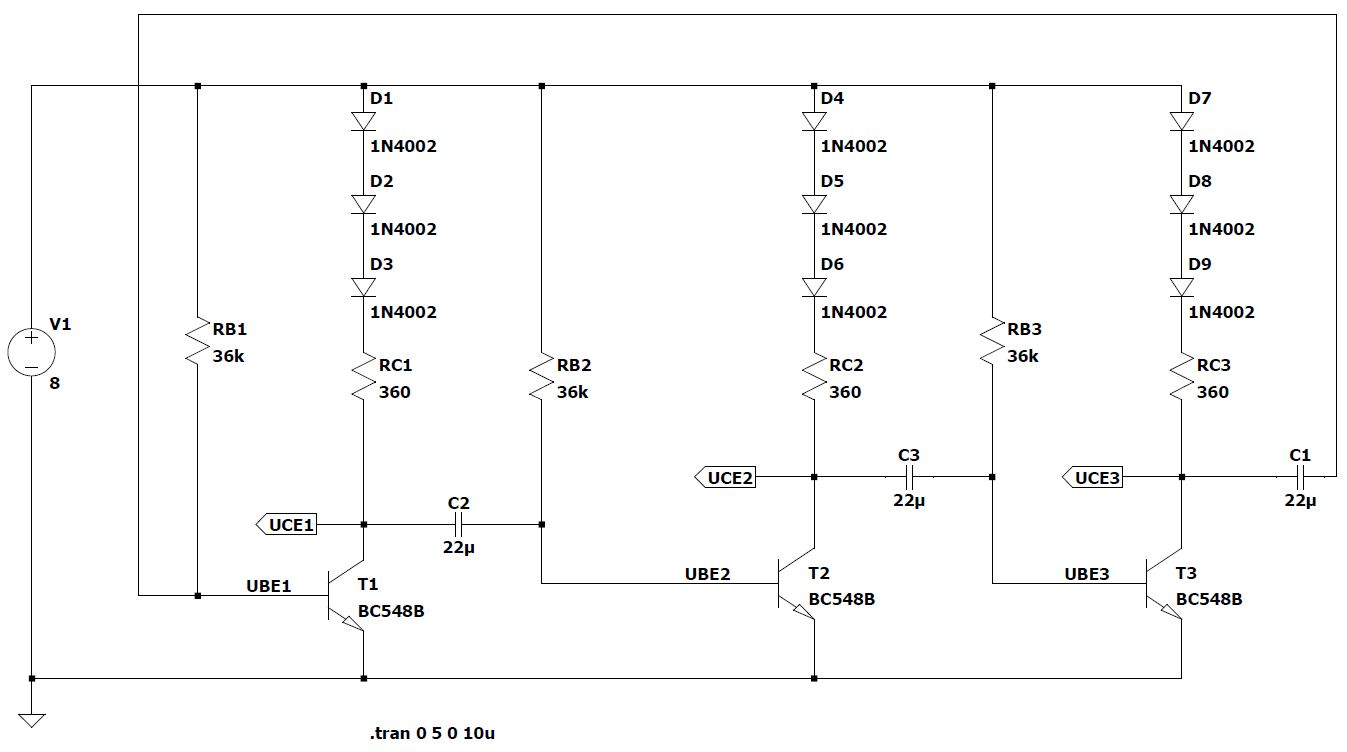
\includegraphics[width = 0.8\textwidth]{\figpath/Kipp_schem_3stufig.jpg}
    \caption{Blinkschaltung mit 3 LEDs}
    \label{fig_Kap3_10:3stufig}
\end{figure}

In Abb. \ref{fig_Kap3_11:Spannungen} können nun die Basis-Emitterspannungen der drei Transistoren betrachtet werden.

\begin{figure}[H]
	\centering \small
	\scalebox{0.9}{% This file was created by matlab2tikz.
%
\definecolor{mycolor1}{rgb}{0.00000,0.44700,0.74100}%
\definecolor{mycolor2}{rgb}{0.85000,0.32500,0.09800}%
\definecolor{mycolor3}{rgb}{0.92900,0.69400,0.12500}%
%
\begin{tikzpicture}

\begin{axis}[%
width=4.521in,
height=3.555in,
at={(0.758in,0.481in)},
scale only axis,
xmin=0,
xmax=5,
xlabel style={font=\color{white!15!black}},
xlabel={$\text{\it{} t \rm{} in s}$},
ymin=-6,
ymax=1,
ylabel style={font=\color{white!15!black}},
ylabel={$\text{\it{} U \rm{} in V}$},
axis background/.style={fill=white},
title style={font=\bfseries},
title={$\text{\it{} U}_{\text{BE}}$},
xmajorgrids,
ymajorgrids,
legend style={legend cell align=left, align=left, draw=white!15!black}
]
\addplot [color=mycolor1]
  table[row sep=crcr]{%
0	0.74\\
0.01	0.74\\
0.02	0.74\\
0.03	0.74\\
0.04	0.74\\
0.05	0.74\\
0.06	0.74\\
0.07	0.74\\
0.08	0.74\\
0.09	0.74\\
0.1	0.74\\
0.11	0.74\\
0.12	0.74\\
0.13	0.74\\
0.14	0.74\\
0.15	0.74\\
0.16	0.74\\
0.17	0.74\\
0.18	0.74\\
0.19	0.74\\
0.2	0.74\\
0.21	0.74\\
0.22	0.74\\
0.23	0.74\\
0.24	0.74\\
0.25	0.75\\
0.26	0.73\\
0.27	0.04\\
0.28	0.14\\
0.29	0.24\\
0.3	0.34\\
0.31	0.44\\
0.32	0.53\\
0.33	0.61\\
0.34	0.64\\
0.35	0.73\\
0.36	0.74\\
0.37	0.74\\
0.38	0.74\\
0.39	0.74\\
0.4	0.74\\
0.41	0.74\\
0.42	0.74\\
0.43	0.74\\
0.44	0.74\\
0.45	0.74\\
0.46	0.74\\
0.47	0.74\\
0.48	0.74\\
0.49	0.74\\
0.5	0.74\\
0.51	0.74\\
0.52	0.74\\
0.53	0.74\\
0.54	0.74\\
0.55	0.74\\
0.56	0.74\\
0.57	0.74\\
0.58	0.74\\
0.59	0.74\\
0.6	0.74\\
0.61	0.74\\
0.62	0.74\\
0.63	0.74\\
0.64	0.74\\
0.65	0.74\\
0.66	0.74\\
0.67	0.74\\
0.68	0.74\\
0.69	0.74\\
0.7	0.74\\
0.71	0.74\\
0.72	0.74\\
0.73	0.74\\
0.74	0.74\\
0.75	0.74\\
0.76	0.74\\
0.77	0.74\\
0.78	0.74\\
0.79	0.74\\
0.8	0.74\\
0.81	0.74\\
0.82	0.74\\
0.83	0.74\\
0.84	0.77\\
0.85	0.75\\
0.86	0.74\\
0.87	0.74\\
0.88	0.74\\
0.89	0.74\\
0.9	0.74\\
0.91	0.74\\
0.92	0.74\\
0.93	0.74\\
0.94	0.74\\
0.95	0.74\\
0.96	0.74\\
0.97	0.74\\
0.98	0.74\\
0.99	0.74\\
1	0.74\\
1.01	0.74\\
1.02	0.74\\
1.03	0.74\\
1.04	0.74\\
1.05	0.74\\
1.06	0.74\\
1.07	0.74\\
1.08	0.74\\
1.09	0.74\\
1.1	0.74\\
1.11	0.74\\
1.12	0.74\\
1.13	0.74\\
1.14	0.74\\
1.15	0.74\\
1.16	0.74\\
1.17	0.74\\
1.18	0.74\\
1.19	0.74\\
1.2	0.74\\
1.21	0.74\\
1.22	0.74\\
1.23	0.74\\
1.24	0.74\\
1.25	0.74\\
1.26	0.74\\
1.27	0.74\\
1.28	0.74\\
1.29	0.74\\
1.3	0.74\\
1.31	0.74\\
1.32	0.74\\
1.33	0.74\\
1.34	0.74\\
1.35	0.74\\
1.36	0.73\\
1.37	-1.12\\
1.38	-5.84\\
1.39	-5.67\\
1.4	-5.5\\
1.41	-5.33\\
1.42	-5.16\\
1.43	-4.99\\
1.44	-4.83\\
1.45	-4.67\\
1.46	-4.51\\
1.47	-4.35\\
1.48	-4.2\\
1.49	-4.04\\
1.5	-3.89\\
1.51	-3.74\\
1.52	-3.6\\
1.53	-3.45\\
1.54	-3.31\\
1.55	-3.16\\
1.56	-3.02\\
1.57	-2.89\\
1.58	-2.75\\
1.59	-2.61\\
1.6	-2.48\\
1.61	-2.35\\
1.62	-2.22\\
1.63	-2.09\\
1.64	-1.97\\
1.65	-1.84\\
1.66	-1.72\\
1.67	-1.59\\
1.68	-1.47\\
1.69	-1.36\\
1.7	-1.24\\
1.71	-1.12\\
1.72	-1.01\\
1.73	-0.89\\
1.74	-0.78\\
1.75	-0.67\\
1.76	-0.56\\
1.77	-0.46\\
1.78	-0.35\\
1.79	-0.25\\
1.8	-0.14\\
1.81	-0.04\\
1.82	0.06\\
1.83	0.16\\
1.84	0.26\\
1.85	0.36\\
1.86	0.45\\
1.87	0.54\\
1.88	0.61\\
1.89	0.65\\
1.9	0.74\\
1.91	0.74\\
1.92	0.74\\
1.93	0.74\\
1.94	0.74\\
1.95	0.74\\
1.96	0.74\\
1.97	0.74\\
1.98	0.74\\
1.99	0.74\\
2	0.74\\
2.01	0.74\\
2.02	0.74\\
2.03	0.74\\
2.04	0.74\\
2.05	0.74\\
2.06	0.74\\
2.07	0.74\\
2.08	0.74\\
2.09	0.74\\
2.1	0.74\\
2.11	0.74\\
2.12	0.74\\
2.13	0.74\\
2.14	0.74\\
2.15	0.74\\
2.16	0.74\\
2.17	0.74\\
2.18	0.74\\
2.19	0.74\\
2.2	0.74\\
2.21	0.74\\
2.22	0.74\\
2.23	0.74\\
2.24	0.74\\
2.25	0.74\\
2.26	0.74\\
2.27	0.74\\
2.28	0.74\\
2.29	0.74\\
2.3	0.74\\
2.31	0.74\\
2.32	0.74\\
2.33	0.74\\
2.34	0.74\\
2.35	0.74\\
2.36	0.74\\
2.37	0.74\\
2.38	0.74\\
2.39	0.74\\
2.4	0.74\\
2.41	0.75\\
2.42	0.76\\
2.43	0.75\\
2.44	0.74\\
2.45	0.74\\
2.46	0.74\\
2.47	0.74\\
2.48	0.74\\
2.49	0.74\\
2.5	0.74\\
2.51	0.74\\
2.52	0.74\\
2.53	0.74\\
2.54	0.74\\
2.55	0.74\\
2.56	0.74\\
2.57	0.74\\
2.58	0.74\\
2.59	0.74\\
2.6	0.74\\
2.61	0.74\\
2.62	0.74\\
2.63	0.74\\
2.64	0.74\\
2.65	0.74\\
2.66	0.74\\
2.67	0.74\\
2.68	0.74\\
2.69	0.74\\
2.7	0.74\\
2.71	0.74\\
2.72	0.74\\
2.73	0.74\\
2.74	0.74\\
2.75	0.74\\
2.76	0.74\\
2.77	0.74\\
2.78	0.74\\
2.79	0.74\\
2.8	0.74\\
2.81	0.74\\
2.82	0.74\\
2.83	0.74\\
2.84	0.74\\
2.85	0.74\\
2.86	0.74\\
2.87	0.74\\
2.88	0.74\\
2.89	0.74\\
2.9	0.74\\
2.91	0.74\\
2.92	0.74\\
2.93	0.74\\
2.94	0.04\\
2.95	-5.91\\
2.96	-5.74\\
2.97	-5.56\\
2.98	-5.39\\
2.99	-5.22\\
3	-5.06\\
3.01	-4.89\\
3.02	-4.73\\
3.03	-4.57\\
3.04	-4.41\\
3.05	-4.26\\
3.06	-4.1\\
3.07	-3.95\\
3.08	-3.8\\
3.09	-3.65\\
3.1	-3.51\\
3.11	-3.36\\
3.12	-3.22\\
3.13	-3.08\\
3.14	-2.94\\
3.15	-2.8\\
3.16	-2.67\\
3.17	-2.53\\
3.18	-2.4\\
3.19	-2.27\\
3.2	-2.14\\
3.21	-2.02\\
3.22	-1.89\\
3.23	-1.77\\
3.24	-1.64\\
3.25	-1.52\\
3.26	-1.4\\
3.27	-1.28\\
3.28	-1.17\\
3.29	-1.05\\
3.3	-0.94\\
3.31	-0.83\\
3.32	-0.72\\
3.33	-0.61\\
3.34	-0.5\\
3.35	-0.39\\
3.36	-0.29\\
3.37	-0.18\\
3.38	-0.08\\
3.39	0.02\\
3.4	0.12\\
3.41	0.22\\
3.42	0.32\\
3.43	0.41\\
3.44	0.51\\
3.45	0.59\\
3.46	0.62\\
3.47	0.71\\
3.48	0.74\\
3.49	0.74\\
3.5	0.74\\
3.51	0.74\\
3.52	0.74\\
3.53	0.74\\
3.54	0.74\\
3.55	0.74\\
3.56	0.74\\
3.57	0.74\\
3.58	0.74\\
3.59	0.74\\
3.6	0.74\\
3.61	0.74\\
3.62	0.74\\
3.63	0.74\\
3.64	0.74\\
3.65	0.74\\
3.66	0.74\\
3.67	0.74\\
3.68	0.74\\
3.69	0.74\\
3.7	0.74\\
3.71	0.74\\
3.72	0.74\\
3.73	0.74\\
3.74	0.74\\
3.75	0.74\\
3.76	0.74\\
3.77	0.74\\
3.78	0.74\\
3.79	0.74\\
3.8	0.74\\
3.81	0.74\\
3.82	0.74\\
3.83	0.74\\
3.84	0.74\\
3.85	0.74\\
3.86	0.74\\
3.87	0.74\\
3.88	0.74\\
3.89	0.74\\
3.9	0.74\\
3.91	0.74\\
3.92	0.74\\
3.93	0.74\\
3.94	0.74\\
3.95	0.74\\
3.96	0.74\\
3.97	0.74\\
3.98	0.74\\
3.99	0.76\\
4	0.75\\
4.01	0.74\\
4.02	0.74\\
4.03	0.74\\
4.04	0.74\\
4.05	0.74\\
4.06	0.74\\
4.07	0.74\\
4.08	0.74\\
4.09	0.74\\
4.1	0.74\\
4.11	0.74\\
4.12	0.74\\
4.13	0.74\\
4.14	0.74\\
4.15	0.74\\
4.16	0.74\\
4.17	0.74\\
4.18	0.74\\
4.19	0.74\\
4.2	0.74\\
4.21	0.74\\
4.22	0.74\\
4.23	0.74\\
4.24	0.74\\
4.25	0.74\\
4.26	0.74\\
4.27	0.74\\
4.28	0.74\\
4.29	0.74\\
4.3	0.74\\
4.31	0.74\\
4.32	0.74\\
4.33	0.74\\
4.34	0.74\\
4.35	0.74\\
4.36	0.74\\
4.37	0.74\\
4.38	0.74\\
4.39	0.74\\
4.4	0.74\\
4.41	0.74\\
4.42	0.74\\
4.43	0.74\\
4.44	0.74\\
4.45	0.74\\
4.46	0.74\\
4.47	0.74\\
4.48	0.74\\
4.49	0.74\\
4.5	0.74\\
4.51	0.72\\
4.52	-2.56\\
4.53	-5.81\\
4.54	-5.63\\
4.55	-5.46\\
4.56	-5.29\\
4.57	-5.12\\
4.58	-4.96\\
4.59	-4.79\\
4.6	-4.63\\
4.61	-4.48\\
4.62	-4.32\\
4.63	-4.16\\
4.64	-4.01\\
4.65	-3.86\\
4.66	-3.71\\
4.67	-3.57\\
4.68	-3.42\\
4.69	-3.28\\
4.7	-3.14\\
4.71	-3\\
4.72	-2.86\\
4.73	-2.72\\
4.74	-2.59\\
4.75	-2.45\\
4.76	-2.32\\
4.77	-2.19\\
4.78	-2.07\\
4.79	-1.94\\
4.8	-1.81\\
4.81	-1.69\\
4.82	-1.57\\
4.83	-1.45\\
4.84	-1.33\\
4.85	-1.21\\
4.86	-1.1\\
4.87	-0.98\\
4.88	-0.87\\
4.89	-0.76\\
4.9	-0.65\\
4.91	-0.54\\
4.92	-0.43\\
4.93	-0.33\\
4.94	-0.22\\
4.95	-0.12\\
4.96	-0.02\\
4.97	0.08\\
4.98	0.18\\
4.99	0.28\\
5	0.38\\
};
\addlegendentry{$\text{U}_{\text{BE1}}$}

\addplot [color=mycolor2]
  table[row sep=crcr]{%
0	0.74\\
0.01	0.74\\
0.02	0.74\\
0.03	0.74\\
0.04	0.74\\
0.05	0.74\\
0.06	0.74\\
0.07	0.74\\
0.08	0.74\\
0.09	0.74\\
0.1	0.74\\
0.11	0.74\\
0.12	0.74\\
0.13	0.74\\
0.14	0.74\\
0.15	0.74\\
0.16	0.74\\
0.17	0.74\\
0.18	0.74\\
0.19	0.74\\
0.2	0.74\\
0.21	0.74\\
0.22	0.74\\
0.23	0.74\\
0.24	0.74\\
0.25	0.74\\
0.26	0.75\\
0.27	0.75\\
0.28	0.75\\
0.29	0.74\\
0.3	0.74\\
0.31	0.74\\
0.32	0.74\\
0.33	0.74\\
0.34	0.72\\
0.35	-3.71\\
0.36	-5.35\\
0.37	-5.18\\
0.38	-5.01\\
0.39	-4.85\\
0.4	-4.69\\
0.41	-4.53\\
0.42	-4.37\\
0.43	-4.22\\
0.44	-4.06\\
0.45	-3.91\\
0.46	-3.76\\
0.47	-3.61\\
0.48	-3.47\\
0.49	-3.32\\
0.5	-3.18\\
0.51	-3.04\\
0.52	-2.9\\
0.53	-2.77\\
0.54	-2.63\\
0.55	-2.5\\
0.56	-2.37\\
0.57	-2.24\\
0.58	-2.11\\
0.59	-1.98\\
0.6	-1.86\\
0.61	-1.73\\
0.62	-1.61\\
0.63	-1.49\\
0.64	-1.37\\
0.65	-1.25\\
0.66	-1.14\\
0.67	-1.02\\
0.68	-0.91\\
0.69	-0.8\\
0.7	-0.69\\
0.71	-0.58\\
0.72	-0.47\\
0.73	-0.36\\
0.74	-0.26\\
0.75	-0.16\\
0.76	-0.05\\
0.77	0.05\\
0.78	0.15\\
0.79	0.25\\
0.8	0.34\\
0.81	0.44\\
0.82	0.53\\
0.83	0.61\\
0.84	0.63\\
0.85	0.73\\
0.86	0.74\\
0.87	0.74\\
0.88	0.74\\
0.89	0.74\\
0.9	0.74\\
0.91	0.74\\
0.92	0.74\\
0.93	0.74\\
0.94	0.74\\
0.95	0.74\\
0.96	0.74\\
0.97	0.74\\
0.98	0.74\\
0.99	0.74\\
1	0.74\\
1.01	0.74\\
1.02	0.74\\
1.03	0.74\\
1.04	0.74\\
1.05	0.74\\
1.06	0.74\\
1.07	0.74\\
1.08	0.74\\
1.09	0.74\\
1.1	0.74\\
1.11	0.74\\
1.12	0.74\\
1.13	0.74\\
1.14	0.74\\
1.15	0.74\\
1.16	0.74\\
1.17	0.74\\
1.18	0.74\\
1.19	0.74\\
1.2	0.74\\
1.21	0.74\\
1.22	0.74\\
1.23	0.74\\
1.24	0.74\\
1.25	0.74\\
1.26	0.74\\
1.27	0.74\\
1.28	0.74\\
1.29	0.74\\
1.3	0.74\\
1.31	0.74\\
1.32	0.74\\
1.33	0.74\\
1.34	0.74\\
1.35	0.74\\
1.36	0.75\\
1.37	0.76\\
1.38	0.75\\
1.39	0.74\\
1.4	0.74\\
1.41	0.74\\
1.42	0.74\\
1.43	0.74\\
1.44	0.74\\
1.45	0.74\\
1.46	0.74\\
1.47	0.74\\
1.48	0.74\\
1.49	0.74\\
1.5	0.74\\
1.51	0.74\\
1.52	0.74\\
1.53	0.74\\
1.54	0.74\\
1.55	0.74\\
1.56	0.74\\
1.57	0.74\\
1.58	0.74\\
1.59	0.74\\
1.6	0.74\\
1.61	0.74\\
1.62	0.74\\
1.63	0.74\\
1.64	0.74\\
1.65	0.74\\
1.66	0.74\\
1.67	0.74\\
1.68	0.74\\
1.69	0.74\\
1.7	0.74\\
1.71	0.74\\
1.72	0.74\\
1.73	0.74\\
1.74	0.74\\
1.75	0.74\\
1.76	0.74\\
1.77	0.74\\
1.78	0.74\\
1.79	0.74\\
1.8	0.74\\
1.81	0.74\\
1.82	0.74\\
1.83	0.74\\
1.84	0.74\\
1.85	0.74\\
1.86	0.74\\
1.87	0.74\\
1.88	0.74\\
1.89	0.16\\
1.9	-5.92\\
1.91	-5.75\\
1.92	-5.58\\
1.93	-5.4\\
1.94	-5.24\\
1.95	-5.07\\
1.96	-4.9\\
1.97	-4.74\\
1.98	-4.58\\
1.99	-4.42\\
2	-4.27\\
2.01	-4.11\\
2.02	-3.96\\
2.03	-3.81\\
2.04	-3.66\\
2.05	-3.52\\
2.06	-3.37\\
2.07	-3.23\\
2.08	-3.09\\
2.09	-2.95\\
2.1	-2.81\\
2.11	-2.68\\
2.12	-2.54\\
2.13	-2.41\\
2.14	-2.28\\
2.15	-2.15\\
2.16	-2.02\\
2.17	-1.9\\
2.18	-1.77\\
2.19	-1.65\\
2.2	-1.53\\
2.21	-1.41\\
2.22	-1.29\\
2.23	-1.18\\
2.24	-1.06\\
2.25	-0.95\\
2.26	-0.84\\
2.27	-0.72\\
2.28	-0.61\\
2.29	-0.51\\
2.3	-0.4\\
2.31	-0.29\\
2.32	-0.19\\
2.33	-0.09\\
2.34	0.01\\
2.35	0.11\\
2.36	0.21\\
2.37	0.31\\
2.38	0.41\\
2.39	0.5\\
2.4	0.59\\
2.41	0.62\\
2.42	0.7\\
2.43	0.74\\
2.44	0.74\\
2.45	0.74\\
2.46	0.74\\
2.47	0.74\\
2.48	0.74\\
2.49	0.74\\
2.5	0.74\\
2.51	0.74\\
2.52	0.74\\
2.53	0.74\\
2.54	0.74\\
2.55	0.74\\
2.56	0.74\\
2.57	0.74\\
2.58	0.74\\
2.59	0.74\\
2.6	0.74\\
2.61	0.74\\
2.62	0.74\\
2.63	0.74\\
2.64	0.74\\
2.65	0.74\\
2.66	0.74\\
2.67	0.74\\
2.68	0.74\\
2.69	0.74\\
2.7	0.74\\
2.71	0.74\\
2.72	0.74\\
2.73	0.74\\
2.74	0.74\\
2.75	0.74\\
2.76	0.74\\
2.77	0.74\\
2.78	0.74\\
2.79	0.74\\
2.8	0.74\\
2.81	0.74\\
2.82	0.74\\
2.83	0.74\\
2.84	0.74\\
2.85	0.74\\
2.86	0.74\\
2.87	0.74\\
2.88	0.74\\
2.89	0.74\\
2.9	0.74\\
2.91	0.74\\
2.92	0.74\\
2.93	0.74\\
2.94	0.76\\
2.95	0.75\\
2.96	0.74\\
2.97	0.74\\
2.98	0.74\\
2.99	0.74\\
3	0.74\\
3.01	0.74\\
3.02	0.74\\
3.03	0.74\\
3.04	0.74\\
3.05	0.74\\
3.06	0.74\\
3.07	0.74\\
3.08	0.74\\
3.09	0.74\\
3.1	0.74\\
3.11	0.74\\
3.12	0.74\\
3.13	0.74\\
3.14	0.74\\
3.15	0.74\\
3.16	0.74\\
3.17	0.74\\
3.18	0.74\\
3.19	0.74\\
3.2	0.74\\
3.21	0.74\\
3.22	0.74\\
3.23	0.74\\
3.24	0.74\\
3.25	0.74\\
3.26	0.74\\
3.27	0.74\\
3.28	0.74\\
3.29	0.74\\
3.3	0.74\\
3.31	0.74\\
3.32	0.74\\
3.33	0.74\\
3.34	0.74\\
3.35	0.74\\
3.36	0.74\\
3.37	0.74\\
3.38	0.74\\
3.39	0.74\\
3.4	0.74\\
3.41	0.74\\
3.42	0.74\\
3.43	0.74\\
3.44	0.74\\
3.45	0.74\\
3.46	0.73\\
3.47	-1.99\\
3.48	-5.82\\
3.49	-5.64\\
3.5	-5.47\\
3.51	-5.3\\
3.52	-5.13\\
3.53	-4.97\\
3.54	-4.81\\
3.55	-4.65\\
3.56	-4.49\\
3.57	-4.33\\
3.58	-4.17\\
3.59	-4.02\\
3.6	-3.87\\
3.61	-3.72\\
3.62	-3.58\\
3.63	-3.43\\
3.64	-3.29\\
3.65	-3.14\\
3.66	-3.01\\
3.67	-2.87\\
3.68	-2.73\\
3.69	-2.6\\
3.7	-2.46\\
3.71	-2.33\\
3.72	-2.2\\
3.73	-2.07\\
3.74	-1.95\\
3.75	-1.82\\
3.76	-1.7\\
3.77	-1.58\\
3.78	-1.46\\
3.79	-1.34\\
3.8	-1.22\\
3.81	-1.11\\
3.82	-0.99\\
3.83	-0.88\\
3.84	-0.77\\
3.85	-0.66\\
3.86	-0.55\\
3.87	-0.44\\
3.88	-0.34\\
3.89	-0.23\\
3.9	-0.13\\
3.91	-0.03\\
3.92	0.07\\
3.93	0.17\\
3.94	0.27\\
3.95	0.37\\
3.96	0.46\\
3.97	0.56\\
3.98	0.61\\
3.99	0.66\\
4	0.74\\
4.01	0.74\\
4.02	0.74\\
4.03	0.74\\
4.04	0.74\\
4.05	0.74\\
4.06	0.74\\
4.07	0.74\\
4.08	0.74\\
4.09	0.74\\
4.1	0.74\\
4.11	0.74\\
4.12	0.74\\
4.13	0.74\\
4.14	0.74\\
4.15	0.74\\
4.16	0.74\\
4.17	0.74\\
4.18	0.74\\
4.19	0.74\\
4.2	0.74\\
4.21	0.74\\
4.22	0.74\\
4.23	0.74\\
4.24	0.74\\
4.25	0.74\\
4.26	0.74\\
4.27	0.74\\
4.28	0.74\\
4.29	0.74\\
4.3	0.74\\
4.31	0.74\\
4.32	0.74\\
4.33	0.74\\
4.34	0.74\\
4.35	0.74\\
4.36	0.74\\
4.37	0.74\\
4.38	0.74\\
4.39	0.74\\
4.4	0.74\\
4.41	0.74\\
4.42	0.74\\
4.43	0.74\\
4.44	0.74\\
4.45	0.74\\
4.46	0.74\\
4.47	0.74\\
4.48	0.74\\
4.49	0.74\\
4.5	0.74\\
4.51	0.76\\
4.52	0.75\\
4.53	0.75\\
4.54	0.74\\
4.55	0.74\\
4.56	0.74\\
4.57	0.74\\
4.58	0.74\\
4.59	0.74\\
4.6	0.74\\
4.61	0.74\\
4.62	0.74\\
4.63	0.74\\
4.64	0.74\\
4.65	0.74\\
4.66	0.74\\
4.67	0.74\\
4.68	0.74\\
4.69	0.74\\
4.7	0.74\\
4.71	0.74\\
4.72	0.74\\
4.73	0.74\\
4.74	0.74\\
4.75	0.74\\
4.76	0.74\\
4.77	0.74\\
4.78	0.74\\
4.79	0.74\\
4.8	0.74\\
4.81	0.74\\
4.82	0.74\\
4.83	0.74\\
4.84	0.74\\
4.85	0.74\\
4.86	0.74\\
4.87	0.74\\
4.88	0.74\\
4.89	0.74\\
4.9	0.74\\
4.91	0.74\\
4.92	0.74\\
4.93	0.74\\
4.94	0.74\\
4.95	0.74\\
4.96	0.74\\
4.97	0.74\\
4.98	0.74\\
4.99	0.74\\
5	0.74\\
};
\addlegendentry{$\text{U}_{\text{BE2}}$}

\addplot [color=mycolor3]
  table[row sep=crcr]{%
0	0.74\\
0.01	0.74\\
0.02	0.74\\
0.03	0.74\\
0.04	0.74\\
0.05	0.74\\
0.06	0.74\\
0.07	0.74\\
0.08	0.74\\
0.09	0.74\\
0.1	0.74\\
0.11	0.74\\
0.12	0.74\\
0.13	0.74\\
0.14	0.74\\
0.15	0.74\\
0.16	0.74\\
0.17	0.74\\
0.18	0.74\\
0.19	0.74\\
0.2	0.74\\
0.21	0.74\\
0.22	0.74\\
0.23	0.74\\
0.24	0.74\\
0.25	0.73\\
0.26	0.74\\
0.27	0.74\\
0.28	0.74\\
0.29	0.74\\
0.3	0.74\\
0.31	0.74\\
0.32	0.74\\
0.33	0.74\\
0.34	0.76\\
0.35	0.75\\
0.36	0.75\\
0.37	0.74\\
0.38	0.74\\
0.39	0.74\\
0.4	0.74\\
0.41	0.74\\
0.42	0.74\\
0.43	0.74\\
0.44	0.74\\
0.45	0.74\\
0.46	0.74\\
0.47	0.74\\
0.48	0.74\\
0.49	0.74\\
0.5	0.74\\
0.51	0.74\\
0.52	0.74\\
0.53	0.74\\
0.54	0.74\\
0.55	0.74\\
0.56	0.74\\
0.57	0.74\\
0.58	0.74\\
0.59	0.74\\
0.6	0.74\\
0.61	0.74\\
0.62	0.74\\
0.63	0.74\\
0.64	0.74\\
0.65	0.74\\
0.66	0.74\\
0.67	0.74\\
0.68	0.74\\
0.69	0.74\\
0.7	0.74\\
0.71	0.74\\
0.72	0.74\\
0.73	0.74\\
0.74	0.74\\
0.75	0.74\\
0.76	0.74\\
0.77	0.74\\
0.78	0.74\\
0.79	0.74\\
0.8	0.74\\
0.81	0.74\\
0.82	0.74\\
0.83	0.74\\
0.84	0.38\\
0.85	-4.89\\
0.86	-5.76\\
0.87	-5.59\\
0.88	-5.42\\
0.89	-5.25\\
0.9	-5.08\\
0.91	-4.92\\
0.92	-4.75\\
0.93	-4.59\\
0.94	-4.44\\
0.95	-4.28\\
0.96	-4.12\\
0.97	-3.97\\
0.98	-3.82\\
0.99	-3.67\\
1	-3.53\\
1.01	-3.38\\
1.02	-3.24\\
1.03	-3.1\\
1.04	-2.96\\
1.05	-2.82\\
1.06	-2.69\\
1.07	-2.55\\
1.08	-2.42\\
1.09	-2.29\\
1.1	-2.16\\
1.11	-2.03\\
1.12	-1.91\\
1.13	-1.78\\
1.14	-1.66\\
1.15	-1.54\\
1.16	-1.42\\
1.17	-1.3\\
1.18	-1.18\\
1.19	-1.07\\
1.2	-0.96\\
1.21	-0.84\\
1.22	-0.73\\
1.23	-0.62\\
1.24	-0.51\\
1.25	-0.41\\
1.26	-0.3\\
1.27	-0.2\\
1.28	-0.09\\
1.29	0.01\\
1.3	0.11\\
1.31	0.21\\
1.32	0.3\\
1.33	0.4\\
1.34	0.5\\
1.35	0.58\\
1.36	0.62\\
1.37	0.69\\
1.38	0.74\\
1.39	0.74\\
1.4	0.74\\
1.41	0.74\\
1.42	0.74\\
1.43	0.74\\
1.44	0.74\\
1.45	0.74\\
1.46	0.74\\
1.47	0.74\\
1.48	0.74\\
1.49	0.74\\
1.5	0.74\\
1.51	0.74\\
1.52	0.74\\
1.53	0.74\\
1.54	0.74\\
1.55	0.74\\
1.56	0.74\\
1.57	0.74\\
1.58	0.74\\
1.59	0.74\\
1.6	0.74\\
1.61	0.74\\
1.62	0.74\\
1.63	0.74\\
1.64	0.74\\
1.65	0.74\\
1.66	0.74\\
1.67	0.74\\
1.68	0.74\\
1.69	0.74\\
1.7	0.74\\
1.71	0.74\\
1.72	0.74\\
1.73	0.74\\
1.74	0.74\\
1.75	0.74\\
1.76	0.74\\
1.77	0.74\\
1.78	0.74\\
1.79	0.74\\
1.8	0.74\\
1.81	0.74\\
1.82	0.74\\
1.83	0.74\\
1.84	0.74\\
1.85	0.74\\
1.86	0.74\\
1.87	0.74\\
1.88	0.74\\
1.89	0.76\\
1.9	0.75\\
1.91	0.74\\
1.92	0.74\\
1.93	0.74\\
1.94	0.74\\
1.95	0.74\\
1.96	0.74\\
1.97	0.74\\
1.98	0.74\\
1.99	0.74\\
2	0.74\\
2.01	0.74\\
2.02	0.74\\
2.03	0.74\\
2.04	0.74\\
2.05	0.74\\
2.06	0.74\\
2.07	0.74\\
2.08	0.74\\
2.09	0.74\\
2.1	0.74\\
2.11	0.74\\
2.12	0.74\\
2.13	0.74\\
2.14	0.74\\
2.15	0.74\\
2.16	0.74\\
2.17	0.74\\
2.18	0.74\\
2.19	0.74\\
2.2	0.74\\
2.21	0.74\\
2.22	0.74\\
2.23	0.74\\
2.24	0.74\\
2.25	0.74\\
2.26	0.74\\
2.27	0.74\\
2.28	0.74\\
2.29	0.74\\
2.3	0.74\\
2.31	0.74\\
2.32	0.74\\
2.33	0.74\\
2.34	0.74\\
2.35	0.74\\
2.36	0.74\\
2.37	0.74\\
2.38	0.74\\
2.39	0.74\\
2.4	0.74\\
2.41	0.73\\
2.42	-1.51\\
2.43	-5.83\\
2.44	-5.66\\
2.45	-5.48\\
2.46	-5.31\\
2.47	-5.15\\
2.48	-4.98\\
2.49	-4.82\\
2.5	-4.66\\
2.51	-4.5\\
2.52	-4.34\\
2.53	-4.19\\
2.54	-4.03\\
2.55	-3.88\\
2.56	-3.73\\
2.57	-3.59\\
2.58	-3.44\\
2.59	-3.3\\
2.6	-3.15\\
2.61	-3.01\\
2.62	-2.88\\
2.63	-2.74\\
2.64	-2.61\\
2.65	-2.47\\
2.66	-2.34\\
2.67	-2.21\\
2.68	-2.08\\
2.69	-1.96\\
2.7	-1.83\\
2.71	-1.71\\
2.72	-1.59\\
2.73	-1.47\\
2.74	-1.35\\
2.75	-1.23\\
2.76	-1.11\\
2.77	-1\\
2.78	-0.89\\
2.79	-0.78\\
2.8	-0.67\\
2.81	-0.56\\
2.82	-0.45\\
2.83	-0.34\\
2.84	-0.24\\
2.85	-0.14\\
2.86	-0.03\\
2.87	0.07\\
2.88	0.17\\
2.89	0.27\\
2.9	0.36\\
2.91	0.46\\
2.92	0.55\\
2.93	0.61\\
2.94	0.65\\
2.95	0.74\\
2.96	0.74\\
2.97	0.74\\
2.98	0.74\\
2.99	0.74\\
3	0.74\\
3.01	0.74\\
3.02	0.74\\
3.03	0.74\\
3.04	0.74\\
3.05	0.74\\
3.06	0.74\\
3.07	0.74\\
3.08	0.74\\
3.09	0.74\\
3.1	0.74\\
3.11	0.74\\
3.12	0.74\\
3.13	0.74\\
3.14	0.74\\
3.15	0.74\\
3.16	0.74\\
3.17	0.74\\
3.18	0.74\\
3.19	0.74\\
3.2	0.74\\
3.21	0.74\\
3.22	0.74\\
3.23	0.74\\
3.24	0.74\\
3.25	0.74\\
3.26	0.74\\
3.27	0.74\\
3.28	0.74\\
3.29	0.74\\
3.3	0.74\\
3.31	0.74\\
3.32	0.74\\
3.33	0.74\\
3.34	0.74\\
3.35	0.74\\
3.36	0.74\\
3.37	0.74\\
3.38	0.74\\
3.39	0.74\\
3.4	0.74\\
3.41	0.74\\
3.42	0.74\\
3.43	0.74\\
3.44	0.74\\
3.45	0.74\\
3.46	0.75\\
3.47	0.75\\
3.48	0.75\\
3.49	0.74\\
3.5	0.74\\
3.51	0.74\\
3.52	0.74\\
3.53	0.74\\
3.54	0.74\\
3.55	0.74\\
3.56	0.74\\
3.57	0.74\\
3.58	0.74\\
3.59	0.74\\
3.6	0.74\\
3.61	0.74\\
3.62	0.74\\
3.63	0.74\\
3.64	0.74\\
3.65	0.74\\
3.66	0.74\\
3.67	0.74\\
3.68	0.74\\
3.69	0.74\\
3.7	0.74\\
3.71	0.74\\
3.72	0.74\\
3.73	0.74\\
3.74	0.74\\
3.75	0.74\\
3.76	0.74\\
3.77	0.74\\
3.78	0.74\\
3.79	0.74\\
3.8	0.74\\
3.81	0.74\\
3.82	0.74\\
3.83	0.74\\
3.84	0.74\\
3.85	0.74\\
3.86	0.74\\
3.87	0.74\\
3.88	0.74\\
3.89	0.74\\
3.9	0.74\\
3.91	0.74\\
3.92	0.74\\
3.93	0.74\\
3.94	0.74\\
3.95	0.74\\
3.96	0.74\\
3.97	0.74\\
3.98	0.74\\
3.99	-0.09\\
4	-5.9\\
4.01	-5.73\\
4.02	-5.55\\
4.03	-5.38\\
4.04	-5.21\\
4.05	-5.05\\
4.06	-4.88\\
4.07	-4.72\\
4.08	-4.56\\
4.09	-4.4\\
4.1	-4.25\\
4.11	-4.09\\
4.12	-3.94\\
4.13	-3.79\\
4.14	-3.64\\
4.15	-3.5\\
4.16	-3.35\\
4.17	-3.21\\
4.18	-3.07\\
4.19	-2.93\\
4.2	-2.79\\
4.21	-2.66\\
4.22	-2.52\\
4.23	-2.39\\
4.24	-2.26\\
4.25	-2.13\\
4.26	-2.01\\
4.27	-1.88\\
4.28	-1.76\\
4.29	-1.63\\
4.3	-1.51\\
4.31	-1.39\\
4.32	-1.28\\
4.33	-1.16\\
4.34	-1.05\\
4.35	-0.93\\
4.36	-0.82\\
4.37	-0.71\\
4.38	-0.6\\
4.39	-0.49\\
4.4	-0.39\\
4.41	-0.28\\
4.42	-0.18\\
4.43	-0.07\\
4.44	0.03\\
4.45	0.13\\
4.46	0.23\\
4.47	0.32\\
4.48	0.42\\
4.49	0.51\\
4.5	0.59\\
4.51	0.62\\
4.52	0.72\\
4.53	0.74\\
4.54	0.74\\
4.55	0.74\\
4.56	0.74\\
4.57	0.74\\
4.58	0.74\\
4.59	0.74\\
4.6	0.74\\
4.61	0.74\\
4.62	0.74\\
4.63	0.74\\
4.64	0.74\\
4.65	0.74\\
4.66	0.74\\
4.67	0.74\\
4.68	0.74\\
4.69	0.74\\
4.7	0.74\\
4.71	0.74\\
4.72	0.74\\
4.73	0.74\\
4.74	0.74\\
4.75	0.74\\
4.76	0.74\\
4.77	0.74\\
4.78	0.74\\
4.79	0.74\\
4.8	0.74\\
4.81	0.74\\
4.82	0.74\\
4.83	0.74\\
4.84	0.74\\
4.85	0.74\\
4.86	0.74\\
4.87	0.74\\
4.88	0.74\\
4.89	0.74\\
4.9	0.74\\
4.91	0.74\\
4.92	0.74\\
4.93	0.74\\
4.94	0.74\\
4.95	0.74\\
4.96	0.74\\
4.97	0.74\\
4.98	0.74\\
4.99	0.74\\
5	0.74\\
};
\addlegendentry{$\text{U}_{\text{BE3}}$}

\end{axis}
\end{tikzpicture}%}
	\caption{Basis-Emitter-Spannungen des 3-Stufigen LED-Blinklichts}
	\label{fig_Kap3_11:Spannungen}
\end{figure}

Anhand der Basis-Emitterspannungen erkennt man, das immer 2 Transistoren leiten, während einer sperrt. Die Dauer der einzelnen Schaltzustände ergibt sich wiederum aus den Ladevorgängen der Basisseitig angebrachten Kondensatoren und beträgt ca. $\SI{0,5}{\second}$.

Nun wird die Schaltung um eine Stufe erweitert, Abb. \ref{fig_Kap3_12:4stufig}.

\begin{figure}[H]
    \centering
    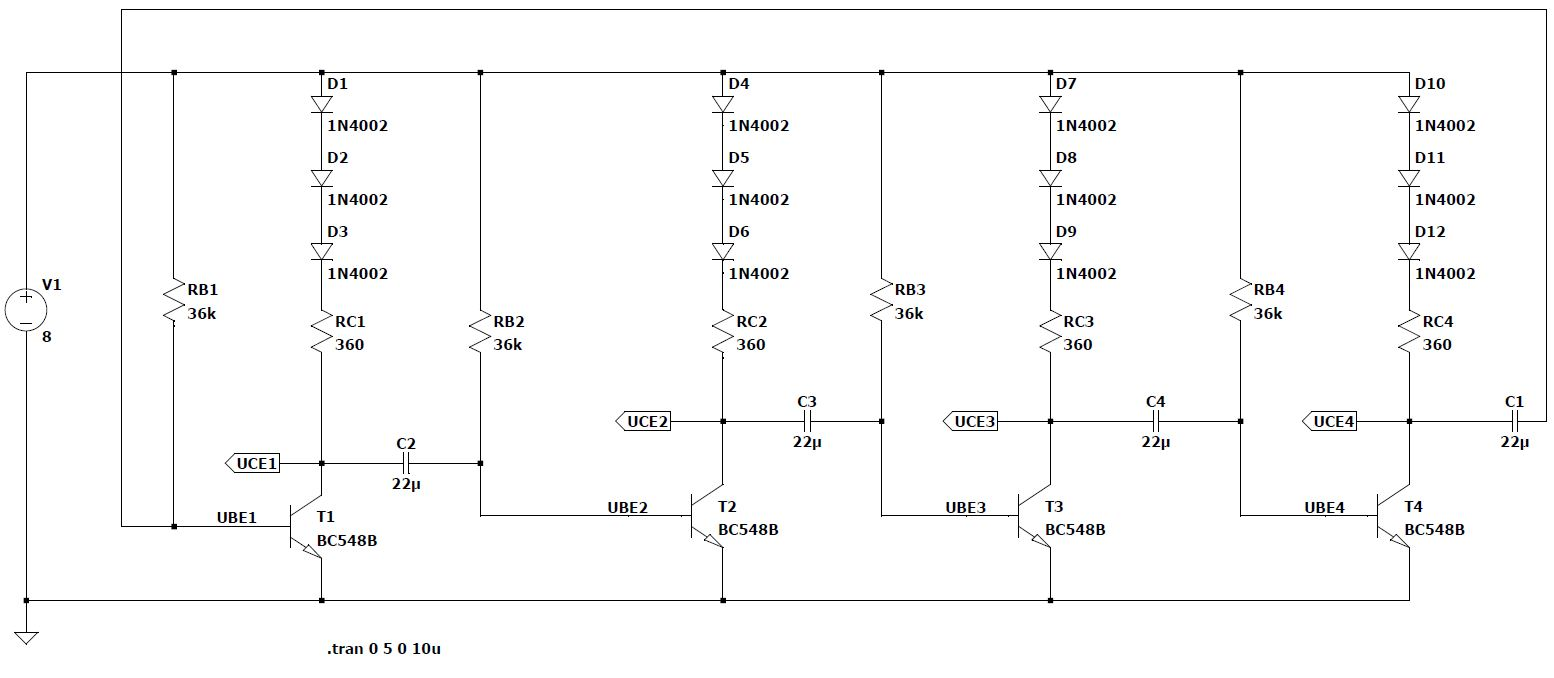
\includegraphics[width = \textwidth]{\figpath/Kipp_schem_4stufig.jpg}
    \caption{4 stufige Schaltung}
    \label{fig_Kap3_12:4stufig}
\end{figure}

\begin{figure}[H]
	\centering \small
	\scalebox{0.9}{% This file was created by matlab2tikz.
%
\definecolor{mycolor1}{rgb}{0.00000,0.44700,0.74100}%
\definecolor{mycolor2}{rgb}{0.85000,0.32500,0.09800}%
\definecolor{mycolor3}{rgb}{0.92900,0.69400,0.12500}%
\definecolor{mycolor4}{rgb}{0.49400,0.18400,0.55600}%
%
\begin{tikzpicture}

\begin{axis}[%
width=4.521in,
height=3.555in,
at={(0.758in,0.481in)},
scale only axis,
xmin=0,
xmax=5,
xlabel style={font=\color{white!15!black}},
xlabel={$t \text{ in s}$},
ymin=-7,
ymax=1,
ylabel style={font=\color{white!15!black}},
ylabel={$U \text{ in V}$},
axis background/.style={fill=white},
title style={font=\bfseries},
title={$U_{BE}$},
xmajorgrids,
ymajorgrids,
legend style={legend cell align=left, align=left, draw=white!15!black}
]
\addplot [color=mycolor1]
  table[row sep=crcr]{%
0	0.74\\
0.01	0.74\\
0.02	0.74\\
0.03	0.74\\
0.04	0.74\\
0.05	0.74\\
0.06	0.74\\
0.07	0.74\\
0.08	0.74\\
0.09	0.74\\
0.1	0.74\\
0.11	0.74\\
0.12	0.35\\
0.13	0.46\\
0.14	0.58\\
0.15	0.76\\
0.16	0.75\\
0.17	0.74\\
0.18	0.74\\
0.19	0.74\\
0.2	0.74\\
0.21	0.74\\
0.22	0.74\\
0.23	0.74\\
0.24	0.74\\
0.25	0.74\\
0.26	0.74\\
0.27	0.74\\
0.28	0.74\\
0.29	0.74\\
0.3	0.74\\
0.31	0.74\\
0.32	0.74\\
0.33	0.74\\
0.34	0.74\\
0.35	0.74\\
0.36	0.74\\
0.37	0.74\\
0.38	0.74\\
0.39	0.74\\
0.4	0.74\\
0.41	0.74\\
0.42	0.74\\
0.43	0.74\\
0.44	0.74\\
0.45	0.74\\
0.46	0.74\\
0.47	0.74\\
0.48	0.74\\
0.49	0.74\\
0.5	0.74\\
0.51	0.74\\
0.52	0.74\\
0.53	0.74\\
0.54	0.74\\
0.55	0.74\\
0.56	0.74\\
0.57	0.74\\
0.58	0.74\\
0.59	0.74\\
0.6	-6.16\\
0.61	-5.96\\
0.62	-5.77\\
0.63	-5.58\\
0.64	-5.4\\
0.65	-5.23\\
0.66	-5.06\\
0.67	-4.89\\
0.68	-4.72\\
0.69	-4.56\\
0.7	-4.4\\
0.71	-4.25\\
0.72	-4.09\\
0.73	-3.94\\
0.74	-3.79\\
0.75	-3.64\\
0.76	-3.5\\
0.77	-3.35\\
0.78	-3.21\\
0.79	-3.07\\
0.8	-2.93\\
0.81	-2.79\\
0.82	-2.66\\
0.83	-2.52\\
0.84	-2.39\\
0.85	-2.26\\
0.86	-2.13\\
0.87	-2\\
0.88	-1.88\\
0.89	-1.75\\
0.9	-1.63\\
0.91	-1.51\\
0.92	-1.39\\
0.93	-1.27\\
0.94	-1.16\\
0.95	-1.04\\
0.96	-0.93\\
0.97	-0.82\\
0.98	-0.71\\
0.99	-0.6\\
1	-0.49\\
1.01	-0.38\\
1.02	-0.28\\
1.03	-0.17\\
1.04	-0.07\\
1.05	0.03\\
1.06	0.13\\
1.07	0.23\\
1.08	0.33\\
1.09	0.42\\
1.1	0.52\\
1.11	0.76\\
1.12	0.75\\
1.13	0.75\\
1.14	0.74\\
1.15	0.74\\
1.16	0.74\\
1.17	0.74\\
1.18	0.74\\
1.19	0.74\\
1.2	0.74\\
1.21	0.74\\
1.22	0.74\\
1.23	0.74\\
1.24	0.74\\
1.25	0.74\\
1.26	0.74\\
1.27	0.74\\
1.28	0.74\\
1.29	0.74\\
1.3	0.74\\
1.31	0.74\\
1.32	0.74\\
1.33	0.74\\
1.34	0.74\\
1.35	0.74\\
1.36	0.74\\
1.37	0.74\\
1.38	0.74\\
1.39	0.74\\
1.4	0.74\\
1.41	0.74\\
1.42	0.74\\
1.43	0.74\\
1.44	0.74\\
1.45	0.74\\
1.46	0.74\\
1.47	0.74\\
1.48	0.74\\
1.49	0.74\\
1.5	0.74\\
1.51	0.74\\
1.52	0.74\\
1.53	0.74\\
1.54	0.74\\
1.55	0.74\\
1.56	0.74\\
1.57	0.74\\
1.58	0.74\\
1.59	0.74\\
1.6	0.74\\
1.61	0.74\\
1.62	-6.17\\
1.63	-5.97\\
1.64	-5.78\\
1.65	-5.59\\
1.66	-5.41\\
1.67	-5.24\\
1.68	-5.07\\
1.69	-4.9\\
1.7	-4.73\\
1.71	-4.57\\
1.72	-4.41\\
1.73	-4.26\\
1.74	-4.1\\
1.75	-3.95\\
1.76	-3.8\\
1.77	-3.65\\
1.78	-3.5\\
1.79	-3.36\\
1.8	-3.22\\
1.81	-3.08\\
1.82	-2.94\\
1.83	-2.8\\
1.84	-2.66\\
1.85	-2.53\\
1.86	-2.4\\
1.87	-2.27\\
1.88	-2.14\\
1.89	-2.01\\
1.9	-1.89\\
1.91	-1.76\\
1.92	-1.64\\
1.93	-1.52\\
1.94	-1.4\\
1.95	-1.28\\
1.96	-1.16\\
1.97	-1.05\\
1.98	-0.94\\
1.99	-0.82\\
2	-0.71\\
2.01	-0.6\\
2.02	-0.49\\
2.03	-0.39\\
2.04	-0.28\\
2.05	-0.18\\
2.06	-0.08\\
2.07	0.02\\
2.08	0.12\\
2.09	0.22\\
2.1	0.32\\
2.11	0.42\\
2.12	0.51\\
2.13	0.76\\
2.14	0.75\\
2.15	0.75\\
2.16	0.74\\
2.17	0.74\\
2.18	0.74\\
2.19	0.74\\
2.2	0.74\\
2.21	0.74\\
2.22	0.74\\
2.23	0.74\\
2.24	0.74\\
2.25	0.74\\
2.26	0.74\\
2.27	0.74\\
2.28	0.74\\
2.29	0.74\\
2.3	0.74\\
2.31	0.74\\
2.32	0.74\\
2.33	0.74\\
2.34	0.74\\
2.35	0.74\\
2.36	0.74\\
2.37	0.74\\
2.38	0.74\\
2.39	0.74\\
2.4	0.74\\
2.41	0.74\\
2.42	0.74\\
2.43	0.74\\
2.44	0.74\\
2.45	0.74\\
2.46	0.74\\
2.47	0.74\\
2.48	0.74\\
2.49	0.74\\
2.5	0.74\\
2.51	0.74\\
2.52	0.74\\
2.53	0.74\\
2.54	0.74\\
2.55	0.74\\
2.56	0.74\\
2.57	0.74\\
2.58	0.74\\
2.59	0.74\\
2.6	0.74\\
2.61	0.74\\
2.62	0.74\\
2.63	0.74\\
2.64	-6.18\\
2.65	-5.98\\
2.66	-5.79\\
2.67	-5.6\\
2.68	-5.42\\
2.69	-5.25\\
2.7	-5.08\\
2.71	-4.91\\
2.72	-4.74\\
2.73	-4.58\\
2.74	-4.42\\
2.75	-4.27\\
2.76	-4.11\\
2.77	-3.96\\
2.78	-3.81\\
2.79	-3.66\\
2.8	-3.51\\
2.81	-3.37\\
2.82	-3.23\\
2.83	-3.08\\
2.84	-2.95\\
2.85	-2.81\\
2.86	-2.67\\
2.87	-2.54\\
2.88	-2.41\\
2.89	-2.28\\
2.9	-2.15\\
2.91	-2.02\\
2.92	-1.89\\
2.93	-1.77\\
2.94	-1.65\\
2.95	-1.53\\
2.96	-1.41\\
2.97	-1.29\\
2.98	-1.17\\
2.99	-1.06\\
3	-0.94\\
3.01	-0.83\\
3.02	-0.72\\
3.03	-0.61\\
3.04	-0.5\\
3.05	-0.39\\
3.06	-0.29\\
3.07	-0.19\\
3.08	-0.08\\
3.09	0.02\\
3.1	0.12\\
3.11	0.22\\
3.12	0.32\\
3.13	0.41\\
3.14	0.51\\
3.15	0.77\\
3.16	0.75\\
3.17	0.75\\
3.18	0.74\\
3.19	0.74\\
3.2	0.74\\
3.21	0.74\\
3.22	0.74\\
3.23	0.74\\
3.24	0.74\\
3.25	0.74\\
3.26	0.74\\
3.27	0.74\\
3.28	0.74\\
3.29	0.74\\
3.3	0.74\\
3.31	0.74\\
3.32	0.74\\
3.33	0.74\\
3.34	0.74\\
3.35	0.74\\
3.36	0.74\\
3.37	0.74\\
3.38	0.74\\
3.39	0.74\\
3.4	0.74\\
3.41	0.74\\
3.42	0.74\\
3.43	0.74\\
3.44	0.74\\
3.45	0.74\\
3.46	0.74\\
3.47	0.74\\
3.48	0.74\\
3.49	0.74\\
3.5	0.74\\
3.51	0.74\\
3.52	0.74\\
3.53	0.74\\
3.54	0.74\\
3.55	0.74\\
3.56	0.74\\
3.57	0.74\\
3.58	0.74\\
3.59	0.74\\
3.6	0.74\\
3.61	0.74\\
3.62	0.74\\
3.63	0.74\\
3.64	0.74\\
3.65	0.74\\
3.66	-6.19\\
3.67	-6\\
3.68	-5.8\\
3.69	-5.61\\
3.7	-5.43\\
3.71	-5.26\\
3.72	-5.09\\
3.73	-4.92\\
3.74	-4.75\\
3.75	-4.59\\
3.76	-4.43\\
3.77	-4.28\\
3.78	-4.12\\
3.79	-3.97\\
3.8	-3.82\\
3.81	-3.67\\
3.82	-3.52\\
3.83	-3.38\\
3.84	-3.23\\
3.85	-3.09\\
3.86	-2.95\\
3.87	-2.82\\
3.88	-2.68\\
3.89	-2.55\\
3.9	-2.41\\
3.91	-2.28\\
3.92	-2.15\\
3.93	-2.03\\
3.94	-1.9\\
3.95	-1.78\\
3.96	-1.65\\
3.97	-1.53\\
3.98	-1.41\\
3.99	-1.29\\
4	-1.18\\
4.01	-1.06\\
4.02	-0.95\\
4.03	-0.84\\
4.04	-0.73\\
4.05	-0.62\\
4.06	-0.51\\
4.07	-0.4\\
4.08	-0.3\\
4.09	-0.19\\
4.1	-0.09\\
4.11	0.01\\
4.12	0.11\\
4.13	0.21\\
4.14	0.31\\
4.15	0.41\\
4.16	0.5\\
4.17	0.77\\
4.18	0.75\\
4.19	0.75\\
4.2	0.74\\
4.21	0.74\\
4.22	0.74\\
4.23	0.74\\
4.24	0.74\\
4.25	0.74\\
4.26	0.74\\
4.27	0.74\\
4.28	0.74\\
4.29	0.74\\
4.3	0.74\\
4.31	0.74\\
4.32	0.74\\
4.33	0.74\\
4.34	0.74\\
4.35	0.74\\
4.36	0.74\\
4.37	0.74\\
4.38	0.74\\
4.39	0.74\\
4.4	0.74\\
4.41	0.74\\
4.42	0.74\\
4.43	0.74\\
4.44	0.74\\
4.45	0.74\\
4.46	0.74\\
4.47	0.74\\
4.48	0.74\\
4.49	0.74\\
4.5	0.74\\
4.51	0.74\\
4.52	0.74\\
4.53	0.74\\
4.54	0.74\\
4.55	0.74\\
4.56	0.74\\
4.57	0.74\\
4.58	0.74\\
4.59	0.74\\
4.6	0.74\\
4.61	0.74\\
4.62	0.74\\
4.63	0.74\\
4.64	0.74\\
4.65	0.74\\
4.66	0.74\\
4.67	0.74\\
4.68	-6.2\\
4.69	-6.01\\
4.7	-5.81\\
4.71	-5.62\\
4.72	-5.44\\
4.73	-5.27\\
4.74	-5.1\\
4.75	-4.93\\
4.76	-4.76\\
4.77	-4.6\\
4.78	-4.44\\
4.79	-4.29\\
4.8	-4.13\\
4.81	-3.98\\
4.82	-3.83\\
4.83	-3.68\\
4.84	-3.53\\
4.85	-3.39\\
4.86	-3.24\\
4.87	-3.1\\
4.88	-2.96\\
4.89	-2.82\\
4.9	-2.69\\
4.91	-2.55\\
4.92	-2.42\\
4.93	-2.29\\
4.94	-2.16\\
4.95	-2.03\\
4.96	-1.91\\
4.97	-1.78\\
4.98	-1.66\\
4.99	-1.54\\
5	-1.42\\
};
\addlegendentry{$\text{U}_{\text{BE1}}$}

\addplot [color=mycolor2]
  table[row sep=crcr]{%
0	0.74\\
0.01	0.74\\
0.02	0.74\\
0.03	0.74\\
0.04	0.74\\
0.05	0.74\\
0.06	0.74\\
0.07	0.74\\
0.08	0.74\\
0.09	0.74\\
0.1	0.74\\
0.11	0.74\\
0.12	0.76\\
0.13	0.75\\
0.14	0.74\\
0.15	-5.14\\
0.16	-4.96\\
0.17	-4.78\\
0.18	-4.6\\
0.19	-4.44\\
0.2	-4.27\\
0.21	-4.12\\
0.22	-3.96\\
0.23	-3.81\\
0.24	-3.66\\
0.25	-3.51\\
0.26	-3.37\\
0.27	-3.22\\
0.28	-3.08\\
0.29	-2.94\\
0.3	-2.81\\
0.31	-2.67\\
0.32	-2.54\\
0.33	-2.4\\
0.34	-2.27\\
0.35	-2.14\\
0.36	-2.02\\
0.37	-1.89\\
0.38	-1.77\\
0.39	-1.64\\
0.4	-1.52\\
0.41	-1.4\\
0.42	-1.28\\
0.43	-1.17\\
0.44	-1.05\\
0.45	-0.94\\
0.46	-0.83\\
0.47	-0.72\\
0.48	-0.61\\
0.49	-0.5\\
0.5	-0.39\\
0.51	-0.29\\
0.52	-0.18\\
0.53	-0.08\\
0.54	0.02\\
0.55	0.12\\
0.56	0.22\\
0.57	0.32\\
0.58	0.42\\
0.59	0.51\\
0.6	0.77\\
0.61	0.75\\
0.62	0.75\\
0.63	0.74\\
0.64	0.74\\
0.65	0.74\\
0.66	0.74\\
0.67	0.74\\
0.68	0.74\\
0.69	0.74\\
0.7	0.74\\
0.71	0.74\\
0.72	0.74\\
0.73	0.74\\
0.74	0.74\\
0.75	0.74\\
0.76	0.74\\
0.77	0.74\\
0.78	0.74\\
0.79	0.74\\
0.8	0.74\\
0.81	0.74\\
0.82	0.74\\
0.83	0.74\\
0.84	0.74\\
0.85	0.74\\
0.86	0.74\\
0.87	0.74\\
0.88	0.74\\
0.89	0.74\\
0.9	0.74\\
0.91	0.74\\
0.92	0.74\\
0.93	0.74\\
0.94	0.74\\
0.95	0.74\\
0.96	0.74\\
0.97	0.74\\
0.98	0.74\\
0.99	0.74\\
1	0.74\\
1.01	0.74\\
1.02	0.74\\
1.03	0.74\\
1.04	0.74\\
1.05	0.74\\
1.06	0.74\\
1.07	0.74\\
1.08	0.74\\
1.09	0.74\\
1.1	0.74\\
1.11	-6.16\\
1.12	-5.97\\
1.13	-5.77\\
1.14	-5.59\\
1.15	-5.4\\
1.16	-5.23\\
1.17	-5.06\\
1.18	-4.89\\
1.19	-4.73\\
1.2	-4.57\\
1.21	-4.41\\
1.22	-4.25\\
1.23	-4.1\\
1.24	-3.95\\
1.25	-3.8\\
1.26	-3.65\\
1.27	-3.5\\
1.28	-3.36\\
1.29	-3.21\\
1.3	-3.07\\
1.31	-2.93\\
1.32	-2.8\\
1.33	-2.66\\
1.34	-2.53\\
1.35	-2.39\\
1.36	-2.26\\
1.37	-2.13\\
1.38	-2.01\\
1.39	-1.88\\
1.4	-1.76\\
1.41	-1.64\\
1.42	-1.51\\
1.43	-1.39\\
1.44	-1.28\\
1.45	-1.16\\
1.46	-1.05\\
1.47	-0.93\\
1.48	-0.82\\
1.49	-0.71\\
1.5	-0.6\\
1.51	-0.49\\
1.52	-0.39\\
1.53	-0.28\\
1.54	-0.18\\
1.55	-0.07\\
1.56	0.03\\
1.57	0.13\\
1.58	0.23\\
1.59	0.32\\
1.6	0.42\\
1.61	0.52\\
1.62	0.76\\
1.63	0.75\\
1.64	0.75\\
1.65	0.74\\
1.66	0.74\\
1.67	0.74\\
1.68	0.74\\
1.69	0.74\\
1.7	0.74\\
1.71	0.74\\
1.72	0.74\\
1.73	0.74\\
1.74	0.74\\
1.75	0.74\\
1.76	0.74\\
1.77	0.74\\
1.78	0.74\\
1.79	0.74\\
1.8	0.74\\
1.81	0.74\\
1.82	0.74\\
1.83	0.74\\
1.84	0.74\\
1.85	0.74\\
1.86	0.74\\
1.87	0.74\\
1.88	0.74\\
1.89	0.74\\
1.9	0.74\\
1.91	0.74\\
1.92	0.74\\
1.93	0.74\\
1.94	0.74\\
1.95	0.74\\
1.96	0.74\\
1.97	0.74\\
1.98	0.74\\
1.99	0.74\\
2	0.74\\
2.01	0.74\\
2.02	0.74\\
2.03	0.74\\
2.04	0.74\\
2.05	0.74\\
2.06	0.74\\
2.07	0.74\\
2.08	0.74\\
2.09	0.74\\
2.1	0.74\\
2.11	0.74\\
2.12	0.74\\
2.13	-6.17\\
2.14	-5.98\\
2.15	-5.78\\
2.16	-5.6\\
2.17	-5.42\\
2.18	-5.24\\
2.19	-5.07\\
2.2	-4.9\\
2.21	-4.74\\
2.22	-4.58\\
2.23	-4.42\\
2.24	-4.26\\
2.25	-4.11\\
2.26	-3.95\\
2.27	-3.8\\
2.28	-3.66\\
2.29	-3.51\\
2.3	-3.36\\
2.31	-3.22\\
2.32	-3.08\\
2.33	-2.94\\
2.34	-2.8\\
2.35	-2.67\\
2.36	-2.53\\
2.37	-2.4\\
2.38	-2.27\\
2.39	-2.14\\
2.4	-2.01\\
2.41	-1.89\\
2.42	-1.77\\
2.43	-1.64\\
2.44	-1.52\\
2.45	-1.4\\
2.46	-1.28\\
2.47	-1.17\\
2.48	-1.05\\
2.49	-0.94\\
2.5	-0.83\\
2.51	-0.72\\
2.52	-0.61\\
2.53	-0.5\\
2.54	-0.39\\
2.55	-0.29\\
2.56	-0.18\\
2.57	-0.08\\
2.58	0.02\\
2.59	0.12\\
2.6	0.22\\
2.61	0.32\\
2.62	0.41\\
2.63	0.51\\
2.64	0.77\\
2.65	0.75\\
2.66	0.75\\
2.67	0.74\\
2.68	0.74\\
2.69	0.74\\
2.7	0.74\\
2.71	0.74\\
2.72	0.74\\
2.73	0.74\\
2.74	0.74\\
2.75	0.74\\
2.76	0.74\\
2.77	0.74\\
2.78	0.74\\
2.79	0.74\\
2.8	0.74\\
2.81	0.74\\
2.82	0.74\\
2.83	0.74\\
2.84	0.74\\
2.85	0.74\\
2.86	0.74\\
2.87	0.74\\
2.88	0.74\\
2.89	0.74\\
2.9	0.74\\
2.91	0.74\\
2.92	0.74\\
2.93	0.74\\
2.94	0.74\\
2.95	0.74\\
2.96	0.74\\
2.97	0.74\\
2.98	0.74\\
2.99	0.74\\
3	0.74\\
3.01	0.74\\
3.02	0.74\\
3.03	0.74\\
3.04	0.74\\
3.05	0.74\\
3.06	0.74\\
3.07	0.74\\
3.08	0.74\\
3.09	0.74\\
3.1	0.74\\
3.11	0.74\\
3.12	0.74\\
3.13	0.74\\
3.14	0.74\\
3.15	-6.18\\
3.16	-5.99\\
3.17	-5.8\\
3.18	-5.61\\
3.19	-5.43\\
3.2	-5.25\\
3.21	-5.08\\
3.22	-4.91\\
3.23	-4.75\\
3.24	-4.59\\
3.25	-4.43\\
3.26	-4.27\\
3.27	-4.12\\
3.28	-3.96\\
3.29	-3.81\\
3.3	-3.66\\
3.31	-3.52\\
3.32	-3.37\\
3.33	-3.23\\
3.34	-3.09\\
3.35	-2.95\\
3.36	-2.81\\
3.37	-2.68\\
3.38	-2.54\\
3.39	-2.41\\
3.4	-2.28\\
3.41	-2.15\\
3.42	-2.02\\
3.43	-1.9\\
3.44	-1.77\\
3.45	-1.65\\
3.46	-1.53\\
3.47	-1.41\\
3.48	-1.29\\
3.49	-1.17\\
3.5	-1.06\\
3.51	-0.95\\
3.52	-0.83\\
3.53	-0.72\\
3.54	-0.61\\
3.55	-0.5\\
3.56	-0.4\\
3.57	-0.29\\
3.58	-0.19\\
3.59	-0.09\\
3.6	0.02\\
3.61	0.12\\
3.62	0.21\\
3.63	0.31\\
3.64	0.41\\
3.65	0.5\\
3.66	0.77\\
3.67	0.75\\
3.68	0.75\\
3.69	0.74\\
3.7	0.74\\
3.71	0.74\\
3.72	0.74\\
3.73	0.74\\
3.74	0.74\\
3.75	0.74\\
3.76	0.74\\
3.77	0.74\\
3.78	0.74\\
3.79	0.74\\
3.8	0.74\\
3.81	0.74\\
3.82	0.74\\
3.83	0.74\\
3.84	0.74\\
3.85	0.74\\
3.86	0.74\\
3.87	0.74\\
3.88	0.74\\
3.89	0.74\\
3.9	0.74\\
3.91	0.74\\
3.92	0.74\\
3.93	0.74\\
3.94	0.74\\
3.95	0.74\\
3.96	0.74\\
3.97	0.74\\
3.98	0.74\\
3.99	0.74\\
4	0.74\\
4.01	0.74\\
4.02	0.74\\
4.03	0.74\\
4.04	0.74\\
4.05	0.74\\
4.06	0.74\\
4.07	0.74\\
4.08	0.74\\
4.09	0.74\\
4.1	0.74\\
4.11	0.74\\
4.12	0.74\\
4.13	0.74\\
4.14	0.74\\
4.15	0.74\\
4.16	0.74\\
4.17	-6.2\\
4.18	-6\\
4.19	-5.81\\
4.2	-5.62\\
4.21	-5.44\\
4.22	-5.26\\
4.23	-5.09\\
4.24	-4.92\\
4.25	-4.76\\
4.26	-4.6\\
4.27	-4.44\\
4.28	-4.28\\
4.29	-4.13\\
4.3	-3.97\\
4.31	-3.82\\
4.32	-3.67\\
4.33	-3.53\\
4.34	-3.38\\
4.35	-3.24\\
4.36	-3.1\\
4.37	-2.96\\
4.38	-2.82\\
4.39	-2.68\\
4.4	-2.55\\
4.41	-2.42\\
4.42	-2.29\\
4.43	-2.16\\
4.44	-2.03\\
4.45	-1.9\\
4.46	-1.78\\
4.47	-1.66\\
4.48	-1.54\\
4.49	-1.42\\
4.5	-1.3\\
4.51	-1.18\\
4.52	-1.07\\
4.53	-0.95\\
4.54	-0.84\\
4.55	-0.73\\
4.56	-0.62\\
4.57	-0.51\\
4.58	-0.4\\
4.59	-0.3\\
4.6	-0.19\\
4.61	-0.09\\
4.62	0.01\\
4.63	0.11\\
4.64	0.21\\
4.65	0.31\\
4.66	0.4\\
4.67	0.5\\
4.68	0.77\\
4.69	0.75\\
4.7	0.75\\
4.71	0.74\\
4.72	0.74\\
4.73	0.74\\
4.74	0.74\\
4.75	0.74\\
4.76	0.74\\
4.77	0.74\\
4.78	0.74\\
4.79	0.74\\
4.8	0.74\\
4.81	0.74\\
4.82	0.74\\
4.83	0.74\\
4.84	0.74\\
4.85	0.74\\
4.86	0.74\\
4.87	0.74\\
4.88	0.74\\
4.89	0.74\\
4.9	0.74\\
4.91	0.74\\
4.92	0.74\\
4.93	0.74\\
4.94	0.74\\
4.95	0.74\\
4.96	0.74\\
4.97	0.74\\
4.98	0.74\\
4.99	0.74\\
5	0.74\\
};
\addlegendentry{$\text{U}_{\text{BE2}}$}

\addplot [color=mycolor3, dashed]
  table[row sep=crcr]{%
0	0.74\\
0.01	0.74\\
0.02	0.74\\
0.03	0.74\\
0.04	0.74\\
0.05	0.74\\
0.06	0.74\\
0.07	0.74\\
0.08	0.74\\
0.09	0.74\\
0.1	0.74\\
0.11	0.74\\
0.12	0.35\\
0.13	0.46\\
0.14	0.58\\
0.15	0.76\\
0.16	0.75\\
0.17	0.74\\
0.18	0.74\\
0.19	0.74\\
0.2	0.74\\
0.21	0.74\\
0.22	0.74\\
0.23	0.74\\
0.24	0.74\\
0.25	0.74\\
0.26	0.74\\
0.27	0.74\\
0.28	0.74\\
0.29	0.74\\
0.3	0.74\\
0.31	0.74\\
0.32	0.74\\
0.33	0.74\\
0.34	0.74\\
0.35	0.74\\
0.36	0.74\\
0.37	0.74\\
0.38	0.74\\
0.39	0.74\\
0.4	0.74\\
0.41	0.74\\
0.42	0.74\\
0.43	0.74\\
0.44	0.74\\
0.45	0.74\\
0.46	0.74\\
0.47	0.74\\
0.48	0.74\\
0.49	0.74\\
0.5	0.74\\
0.51	0.74\\
0.52	0.74\\
0.53	0.74\\
0.54	0.74\\
0.55	0.74\\
0.56	0.74\\
0.57	0.74\\
0.58	0.74\\
0.59	0.74\\
0.6	-6.16\\
0.61	-5.96\\
0.62	-5.77\\
0.63	-5.58\\
0.64	-5.4\\
0.65	-5.23\\
0.66	-5.06\\
0.67	-4.89\\
0.68	-4.72\\
0.69	-4.56\\
0.7	-4.4\\
0.71	-4.25\\
0.72	-4.09\\
0.73	-3.94\\
0.74	-3.79\\
0.75	-3.64\\
0.76	-3.5\\
0.77	-3.35\\
0.78	-3.21\\
0.79	-3.07\\
0.8	-2.93\\
0.81	-2.79\\
0.82	-2.66\\
0.83	-2.52\\
0.84	-2.39\\
0.85	-2.26\\
0.86	-2.13\\
0.87	-2\\
0.88	-1.88\\
0.89	-1.75\\
0.9	-1.63\\
0.91	-1.51\\
0.92	-1.39\\
0.93	-1.27\\
0.94	-1.16\\
0.95	-1.04\\
0.96	-0.93\\
0.97	-0.82\\
0.98	-0.71\\
0.99	-0.6\\
1	-0.49\\
1.01	-0.38\\
1.02	-0.28\\
1.03	-0.17\\
1.04	-0.07\\
1.05	0.03\\
1.06	0.13\\
1.07	0.23\\
1.08	0.33\\
1.09	0.42\\
1.1	0.52\\
1.11	0.76\\
1.12	0.75\\
1.13	0.75\\
1.14	0.74\\
1.15	0.74\\
1.16	0.74\\
1.17	0.74\\
1.18	0.74\\
1.19	0.74\\
1.2	0.74\\
1.21	0.74\\
1.22	0.74\\
1.23	0.74\\
1.24	0.74\\
1.25	0.74\\
1.26	0.74\\
1.27	0.74\\
1.28	0.74\\
1.29	0.74\\
1.3	0.74\\
1.31	0.74\\
1.32	0.74\\
1.33	0.74\\
1.34	0.74\\
1.35	0.74\\
1.36	0.74\\
1.37	0.74\\
1.38	0.74\\
1.39	0.74\\
1.4	0.74\\
1.41	0.74\\
1.42	0.74\\
1.43	0.74\\
1.44	0.74\\
1.45	0.74\\
1.46	0.74\\
1.47	0.74\\
1.48	0.74\\
1.49	0.74\\
1.5	0.74\\
1.51	0.74\\
1.52	0.74\\
1.53	0.74\\
1.54	0.74\\
1.55	0.74\\
1.56	0.74\\
1.57	0.74\\
1.58	0.74\\
1.59	0.74\\
1.6	0.74\\
1.61	0.74\\
1.62	-6.17\\
1.63	-5.97\\
1.64	-5.78\\
1.65	-5.59\\
1.66	-5.41\\
1.67	-5.24\\
1.68	-5.07\\
1.69	-4.9\\
1.7	-4.73\\
1.71	-4.57\\
1.72	-4.41\\
1.73	-4.26\\
1.74	-4.1\\
1.75	-3.95\\
1.76	-3.8\\
1.77	-3.65\\
1.78	-3.5\\
1.79	-3.36\\
1.8	-3.22\\
1.81	-3.08\\
1.82	-2.94\\
1.83	-2.8\\
1.84	-2.66\\
1.85	-2.53\\
1.86	-2.4\\
1.87	-2.27\\
1.88	-2.14\\
1.89	-2.01\\
1.9	-1.89\\
1.91	-1.76\\
1.92	-1.64\\
1.93	-1.52\\
1.94	-1.4\\
1.95	-1.28\\
1.96	-1.16\\
1.97	-1.05\\
1.98	-0.94\\
1.99	-0.82\\
2	-0.71\\
2.01	-0.6\\
2.02	-0.49\\
2.03	-0.39\\
2.04	-0.28\\
2.05	-0.18\\
2.06	-0.08\\
2.07	0.02\\
2.08	0.12\\
2.09	0.22\\
2.1	0.32\\
2.11	0.42\\
2.12	0.51\\
2.13	0.76\\
2.14	0.75\\
2.15	0.75\\
2.16	0.74\\
2.17	0.74\\
2.18	0.74\\
2.19	0.74\\
2.2	0.74\\
2.21	0.74\\
2.22	0.74\\
2.23	0.74\\
2.24	0.74\\
2.25	0.74\\
2.26	0.74\\
2.27	0.74\\
2.28	0.74\\
2.29	0.74\\
2.3	0.74\\
2.31	0.74\\
2.32	0.74\\
2.33	0.74\\
2.34	0.74\\
2.35	0.74\\
2.36	0.74\\
2.37	0.74\\
2.38	0.74\\
2.39	0.74\\
2.4	0.74\\
2.41	0.74\\
2.42	0.74\\
2.43	0.74\\
2.44	0.74\\
2.45	0.74\\
2.46	0.74\\
2.47	0.74\\
2.48	0.74\\
2.49	0.74\\
2.5	0.74\\
2.51	0.74\\
2.52	0.74\\
2.53	0.74\\
2.54	0.74\\
2.55	0.74\\
2.56	0.74\\
2.57	0.74\\
2.58	0.74\\
2.59	0.74\\
2.6	0.74\\
2.61	0.74\\
2.62	0.74\\
2.63	0.74\\
2.64	-6.18\\
2.65	-5.98\\
2.66	-5.79\\
2.67	-5.6\\
2.68	-5.42\\
2.69	-5.25\\
2.7	-5.08\\
2.71	-4.91\\
2.72	-4.74\\
2.73	-4.58\\
2.74	-4.42\\
2.75	-4.27\\
2.76	-4.11\\
2.77	-3.96\\
2.78	-3.81\\
2.79	-3.66\\
2.8	-3.51\\
2.81	-3.37\\
2.82	-3.23\\
2.83	-3.08\\
2.84	-2.95\\
2.85	-2.81\\
2.86	-2.67\\
2.87	-2.54\\
2.88	-2.41\\
2.89	-2.28\\
2.9	-2.15\\
2.91	-2.02\\
2.92	-1.89\\
2.93	-1.77\\
2.94	-1.65\\
2.95	-1.53\\
2.96	-1.41\\
2.97	-1.29\\
2.98	-1.17\\
2.99	-1.06\\
3	-0.94\\
3.01	-0.83\\
3.02	-0.72\\
3.03	-0.61\\
3.04	-0.5\\
3.05	-0.39\\
3.06	-0.29\\
3.07	-0.19\\
3.08	-0.08\\
3.09	0.02\\
3.1	0.12\\
3.11	0.22\\
3.12	0.32\\
3.13	0.41\\
3.14	0.51\\
3.15	0.77\\
3.16	0.75\\
3.17	0.75\\
3.18	0.74\\
3.19	0.74\\
3.2	0.74\\
3.21	0.74\\
3.22	0.74\\
3.23	0.74\\
3.24	0.74\\
3.25	0.74\\
3.26	0.74\\
3.27	0.74\\
3.28	0.74\\
3.29	0.74\\
3.3	0.74\\
3.31	0.74\\
3.32	0.74\\
3.33	0.74\\
3.34	0.74\\
3.35	0.74\\
3.36	0.74\\
3.37	0.74\\
3.38	0.74\\
3.39	0.74\\
3.4	0.74\\
3.41	0.74\\
3.42	0.74\\
3.43	0.74\\
3.44	0.74\\
3.45	0.74\\
3.46	0.74\\
3.47	0.74\\
3.48	0.74\\
3.49	0.74\\
3.5	0.74\\
3.51	0.74\\
3.52	0.74\\
3.53	0.74\\
3.54	0.74\\
3.55	0.74\\
3.56	0.74\\
3.57	0.74\\
3.58	0.74\\
3.59	0.74\\
3.6	0.74\\
3.61	0.74\\
3.62	0.74\\
3.63	0.74\\
3.64	0.74\\
3.65	0.74\\
3.66	-6.19\\
3.67	-6\\
3.68	-5.8\\
3.69	-5.61\\
3.7	-5.43\\
3.71	-5.26\\
3.72	-5.09\\
3.73	-4.92\\
3.74	-4.75\\
3.75	-4.59\\
3.76	-4.43\\
3.77	-4.28\\
3.78	-4.12\\
3.79	-3.97\\
3.8	-3.82\\
3.81	-3.67\\
3.82	-3.52\\
3.83	-3.38\\
3.84	-3.23\\
3.85	-3.09\\
3.86	-2.95\\
3.87	-2.82\\
3.88	-2.68\\
3.89	-2.55\\
3.9	-2.41\\
3.91	-2.28\\
3.92	-2.15\\
3.93	-2.03\\
3.94	-1.9\\
3.95	-1.78\\
3.96	-1.65\\
3.97	-1.53\\
3.98	-1.41\\
3.99	-1.29\\
4	-1.18\\
4.01	-1.06\\
4.02	-0.95\\
4.03	-0.84\\
4.04	-0.73\\
4.05	-0.62\\
4.06	-0.51\\
4.07	-0.4\\
4.08	-0.3\\
4.09	-0.19\\
4.1	-0.09\\
4.11	0.01\\
4.12	0.11\\
4.13	0.21\\
4.14	0.31\\
4.15	0.41\\
4.16	0.5\\
4.17	0.77\\
4.18	0.75\\
4.19	0.75\\
4.2	0.74\\
4.21	0.74\\
4.22	0.74\\
4.23	0.74\\
4.24	0.74\\
4.25	0.74\\
4.26	0.74\\
4.27	0.74\\
4.28	0.74\\
4.29	0.74\\
4.3	0.74\\
4.31	0.74\\
4.32	0.74\\
4.33	0.74\\
4.34	0.74\\
4.35	0.74\\
4.36	0.74\\
4.37	0.74\\
4.38	0.74\\
4.39	0.74\\
4.4	0.74\\
4.41	0.74\\
4.42	0.74\\
4.43	0.74\\
4.44	0.74\\
4.45	0.74\\
4.46	0.74\\
4.47	0.74\\
4.48	0.74\\
4.49	0.74\\
4.5	0.74\\
4.51	0.74\\
4.52	0.74\\
4.53	0.74\\
4.54	0.74\\
4.55	0.74\\
4.56	0.74\\
4.57	0.74\\
4.58	0.74\\
4.59	0.74\\
4.6	0.74\\
4.61	0.74\\
4.62	0.74\\
4.63	0.74\\
4.64	0.74\\
4.65	0.74\\
4.66	0.74\\
4.67	0.74\\
4.68	-6.2\\
4.69	-6.01\\
4.7	-5.81\\
4.71	-5.62\\
4.72	-5.44\\
4.73	-5.27\\
4.74	-5.1\\
4.75	-4.93\\
4.76	-4.76\\
4.77	-4.6\\
4.78	-4.44\\
4.79	-4.29\\
4.8	-4.13\\
4.81	-3.98\\
4.82	-3.83\\
4.83	-3.68\\
4.84	-3.53\\
4.85	-3.39\\
4.86	-3.24\\
4.87	-3.1\\
4.88	-2.96\\
4.89	-2.82\\
4.9	-2.69\\
4.91	-2.55\\
4.92	-2.42\\
4.93	-2.29\\
4.94	-2.16\\
4.95	-2.03\\
4.96	-1.91\\
4.97	-1.78\\
4.98	-1.66\\
4.99	-1.54\\
5	-1.42\\
};
\addlegendentry{$\text{U}_{\text{BE3}}$}

\addplot [color=mycolor4, dashed]
  table[row sep=crcr]{%
0	0.74\\
0.01	0.74\\
0.02	0.74\\
0.03	0.74\\
0.04	0.74\\
0.05	0.74\\
0.06	0.74\\
0.07	0.74\\
0.08	0.74\\
0.09	0.74\\
0.1	0.74\\
0.11	0.74\\
0.12	0.76\\
0.13	0.75\\
0.14	0.74\\
0.15	-5.14\\
0.16	-4.96\\
0.17	-4.78\\
0.18	-4.6\\
0.19	-4.44\\
0.2	-4.27\\
0.21	-4.12\\
0.22	-3.96\\
0.23	-3.81\\
0.24	-3.66\\
0.25	-3.51\\
0.26	-3.37\\
0.27	-3.22\\
0.28	-3.08\\
0.29	-2.94\\
0.3	-2.81\\
0.31	-2.67\\
0.32	-2.54\\
0.33	-2.4\\
0.34	-2.27\\
0.35	-2.14\\
0.36	-2.02\\
0.37	-1.89\\
0.38	-1.77\\
0.39	-1.64\\
0.4	-1.52\\
0.41	-1.4\\
0.42	-1.28\\
0.43	-1.17\\
0.44	-1.05\\
0.45	-0.94\\
0.46	-0.83\\
0.47	-0.72\\
0.48	-0.61\\
0.49	-0.5\\
0.5	-0.39\\
0.51	-0.29\\
0.52	-0.18\\
0.53	-0.08\\
0.54	0.02\\
0.55	0.12\\
0.56	0.22\\
0.57	0.32\\
0.58	0.42\\
0.59	0.51\\
0.6	0.77\\
0.61	0.75\\
0.62	0.75\\
0.63	0.74\\
0.64	0.74\\
0.65	0.74\\
0.66	0.74\\
0.67	0.74\\
0.68	0.74\\
0.69	0.74\\
0.7	0.74\\
0.71	0.74\\
0.72	0.74\\
0.73	0.74\\
0.74	0.74\\
0.75	0.74\\
0.76	0.74\\
0.77	0.74\\
0.78	0.74\\
0.79	0.74\\
0.8	0.74\\
0.81	0.74\\
0.82	0.74\\
0.83	0.74\\
0.84	0.74\\
0.85	0.74\\
0.86	0.74\\
0.87	0.74\\
0.88	0.74\\
0.89	0.74\\
0.9	0.74\\
0.91	0.74\\
0.92	0.74\\
0.93	0.74\\
0.94	0.74\\
0.95	0.74\\
0.96	0.74\\
0.97	0.74\\
0.98	0.74\\
0.99	0.74\\
1	0.74\\
1.01	0.74\\
1.02	0.74\\
1.03	0.74\\
1.04	0.74\\
1.05	0.74\\
1.06	0.74\\
1.07	0.74\\
1.08	0.74\\
1.09	0.74\\
1.1	0.74\\
1.11	-6.16\\
1.12	-5.97\\
1.13	-5.77\\
1.14	-5.59\\
1.15	-5.4\\
1.16	-5.23\\
1.17	-5.06\\
1.18	-4.89\\
1.19	-4.73\\
1.2	-4.57\\
1.21	-4.41\\
1.22	-4.25\\
1.23	-4.1\\
1.24	-3.95\\
1.25	-3.8\\
1.26	-3.65\\
1.27	-3.5\\
1.28	-3.36\\
1.29	-3.21\\
1.3	-3.07\\
1.31	-2.93\\
1.32	-2.8\\
1.33	-2.66\\
1.34	-2.53\\
1.35	-2.39\\
1.36	-2.26\\
1.37	-2.13\\
1.38	-2.01\\
1.39	-1.88\\
1.4	-1.76\\
1.41	-1.64\\
1.42	-1.51\\
1.43	-1.39\\
1.44	-1.28\\
1.45	-1.16\\
1.46	-1.05\\
1.47	-0.93\\
1.48	-0.82\\
1.49	-0.71\\
1.5	-0.6\\
1.51	-0.49\\
1.52	-0.39\\
1.53	-0.28\\
1.54	-0.18\\
1.55	-0.07\\
1.56	0.03\\
1.57	0.13\\
1.58	0.23\\
1.59	0.32\\
1.6	0.42\\
1.61	0.52\\
1.62	0.76\\
1.63	0.75\\
1.64	0.75\\
1.65	0.74\\
1.66	0.74\\
1.67	0.74\\
1.68	0.74\\
1.69	0.74\\
1.7	0.74\\
1.71	0.74\\
1.72	0.74\\
1.73	0.74\\
1.74	0.74\\
1.75	0.74\\
1.76	0.74\\
1.77	0.74\\
1.78	0.74\\
1.79	0.74\\
1.8	0.74\\
1.81	0.74\\
1.82	0.74\\
1.83	0.74\\
1.84	0.74\\
1.85	0.74\\
1.86	0.74\\
1.87	0.74\\
1.88	0.74\\
1.89	0.74\\
1.9	0.74\\
1.91	0.74\\
1.92	0.74\\
1.93	0.74\\
1.94	0.74\\
1.95	0.74\\
1.96	0.74\\
1.97	0.74\\
1.98	0.74\\
1.99	0.74\\
2	0.74\\
2.01	0.74\\
2.02	0.74\\
2.03	0.74\\
2.04	0.74\\
2.05	0.74\\
2.06	0.74\\
2.07	0.74\\
2.08	0.74\\
2.09	0.74\\
2.1	0.74\\
2.11	0.74\\
2.12	0.74\\
2.13	-6.17\\
2.14	-5.98\\
2.15	-5.78\\
2.16	-5.6\\
2.17	-5.42\\
2.18	-5.24\\
2.19	-5.07\\
2.2	-4.9\\
2.21	-4.74\\
2.22	-4.58\\
2.23	-4.42\\
2.24	-4.26\\
2.25	-4.11\\
2.26	-3.95\\
2.27	-3.8\\
2.28	-3.66\\
2.29	-3.51\\
2.3	-3.36\\
2.31	-3.22\\
2.32	-3.08\\
2.33	-2.94\\
2.34	-2.8\\
2.35	-2.67\\
2.36	-2.53\\
2.37	-2.4\\
2.38	-2.27\\
2.39	-2.14\\
2.4	-2.01\\
2.41	-1.89\\
2.42	-1.77\\
2.43	-1.64\\
2.44	-1.52\\
2.45	-1.4\\
2.46	-1.28\\
2.47	-1.17\\
2.48	-1.05\\
2.49	-0.94\\
2.5	-0.83\\
2.51	-0.72\\
2.52	-0.61\\
2.53	-0.5\\
2.54	-0.39\\
2.55	-0.29\\
2.56	-0.18\\
2.57	-0.08\\
2.58	0.02\\
2.59	0.12\\
2.6	0.22\\
2.61	0.32\\
2.62	0.41\\
2.63	0.51\\
2.64	0.77\\
2.65	0.75\\
2.66	0.75\\
2.67	0.74\\
2.68	0.74\\
2.69	0.74\\
2.7	0.74\\
2.71	0.74\\
2.72	0.74\\
2.73	0.74\\
2.74	0.74\\
2.75	0.74\\
2.76	0.74\\
2.77	0.74\\
2.78	0.74\\
2.79	0.74\\
2.8	0.74\\
2.81	0.74\\
2.82	0.74\\
2.83	0.74\\
2.84	0.74\\
2.85	0.74\\
2.86	0.74\\
2.87	0.74\\
2.88	0.74\\
2.89	0.74\\
2.9	0.74\\
2.91	0.74\\
2.92	0.74\\
2.93	0.74\\
2.94	0.74\\
2.95	0.74\\
2.96	0.74\\
2.97	0.74\\
2.98	0.74\\
2.99	0.74\\
3	0.74\\
3.01	0.74\\
3.02	0.74\\
3.03	0.74\\
3.04	0.74\\
3.05	0.74\\
3.06	0.74\\
3.07	0.74\\
3.08	0.74\\
3.09	0.74\\
3.1	0.74\\
3.11	0.74\\
3.12	0.74\\
3.13	0.74\\
3.14	0.74\\
3.15	-6.18\\
3.16	-5.99\\
3.17	-5.8\\
3.18	-5.61\\
3.19	-5.43\\
3.2	-5.25\\
3.21	-5.08\\
3.22	-4.91\\
3.23	-4.75\\
3.24	-4.59\\
3.25	-4.43\\
3.26	-4.27\\
3.27	-4.12\\
3.28	-3.96\\
3.29	-3.81\\
3.3	-3.66\\
3.31	-3.52\\
3.32	-3.37\\
3.33	-3.23\\
3.34	-3.09\\
3.35	-2.95\\
3.36	-2.81\\
3.37	-2.68\\
3.38	-2.54\\
3.39	-2.41\\
3.4	-2.28\\
3.41	-2.15\\
3.42	-2.02\\
3.43	-1.9\\
3.44	-1.77\\
3.45	-1.65\\
3.46	-1.53\\
3.47	-1.41\\
3.48	-1.29\\
3.49	-1.17\\
3.5	-1.06\\
3.51	-0.95\\
3.52	-0.83\\
3.53	-0.72\\
3.54	-0.61\\
3.55	-0.5\\
3.56	-0.4\\
3.57	-0.29\\
3.58	-0.19\\
3.59	-0.09\\
3.6	0.02\\
3.61	0.12\\
3.62	0.21\\
3.63	0.31\\
3.64	0.41\\
3.65	0.5\\
3.66	0.77\\
3.67	0.75\\
3.68	0.75\\
3.69	0.74\\
3.7	0.74\\
3.71	0.74\\
3.72	0.74\\
3.73	0.74\\
3.74	0.74\\
3.75	0.74\\
3.76	0.74\\
3.77	0.74\\
3.78	0.74\\
3.79	0.74\\
3.8	0.74\\
3.81	0.74\\
3.82	0.74\\
3.83	0.74\\
3.84	0.74\\
3.85	0.74\\
3.86	0.74\\
3.87	0.74\\
3.88	0.74\\
3.89	0.74\\
3.9	0.74\\
3.91	0.74\\
3.92	0.74\\
3.93	0.74\\
3.94	0.74\\
3.95	0.74\\
3.96	0.74\\
3.97	0.74\\
3.98	0.74\\
3.99	0.74\\
4	0.74\\
4.01	0.74\\
4.02	0.74\\
4.03	0.74\\
4.04	0.74\\
4.05	0.74\\
4.06	0.74\\
4.07	0.74\\
4.08	0.74\\
4.09	0.74\\
4.1	0.74\\
4.11	0.74\\
4.12	0.74\\
4.13	0.74\\
4.14	0.74\\
4.15	0.74\\
4.16	0.74\\
4.17	-6.2\\
4.18	-6\\
4.19	-5.81\\
4.2	-5.62\\
4.21	-5.44\\
4.22	-5.26\\
4.23	-5.09\\
4.24	-4.92\\
4.25	-4.76\\
4.26	-4.6\\
4.27	-4.44\\
4.28	-4.28\\
4.29	-4.13\\
4.3	-3.97\\
4.31	-3.82\\
4.32	-3.67\\
4.33	-3.53\\
4.34	-3.38\\
4.35	-3.24\\
4.36	-3.1\\
4.37	-2.96\\
4.38	-2.82\\
4.39	-2.68\\
4.4	-2.55\\
4.41	-2.42\\
4.42	-2.29\\
4.43	-2.16\\
4.44	-2.03\\
4.45	-1.9\\
4.46	-1.78\\
4.47	-1.66\\
4.48	-1.54\\
4.49	-1.42\\
4.5	-1.3\\
4.51	-1.18\\
4.52	-1.07\\
4.53	-0.95\\
4.54	-0.84\\
4.55	-0.73\\
4.56	-0.62\\
4.57	-0.51\\
4.58	-0.4\\
4.59	-0.3\\
4.6	-0.19\\
4.61	-0.09\\
4.62	0.01\\
4.63	0.11\\
4.64	0.21\\
4.65	0.31\\
4.66	0.4\\
4.67	0.5\\
4.68	0.77\\
4.69	0.75\\
4.7	0.75\\
4.71	0.74\\
4.72	0.74\\
4.73	0.74\\
4.74	0.74\\
4.75	0.74\\
4.76	0.74\\
4.77	0.74\\
4.78	0.74\\
4.79	0.74\\
4.8	0.74\\
4.81	0.74\\
4.82	0.74\\
4.83	0.74\\
4.84	0.74\\
4.85	0.74\\
4.86	0.74\\
4.87	0.74\\
4.88	0.74\\
4.89	0.74\\
4.9	0.74\\
4.91	0.74\\
4.92	0.74\\
4.93	0.74\\
4.94	0.74\\
4.95	0.74\\
4.96	0.74\\
4.97	0.74\\
4.98	0.74\\
4.99	0.74\\
5	0.74\\
};
\addlegendentry{$\text{U}_{\text{BE4}}$}

\end{axis}
\end{tikzpicture}%}
	\caption{Basis-Emitter-Spannungen des 4-Stufigen LED-Blinklichts}
	\label{fig_Kap3_13:Spannungen}
\end{figure}

Die Schaltung funktioniert also nicht als 4-stufiges Lauflicht. Nun stellt sich die Frage, ob trotzdem eine Erweiterung auf 5 Stufen möglich ist, siehe Abb. \ref{fig_Kap3_14:5stufig}.

\begin{figure}[H]
    \centering
    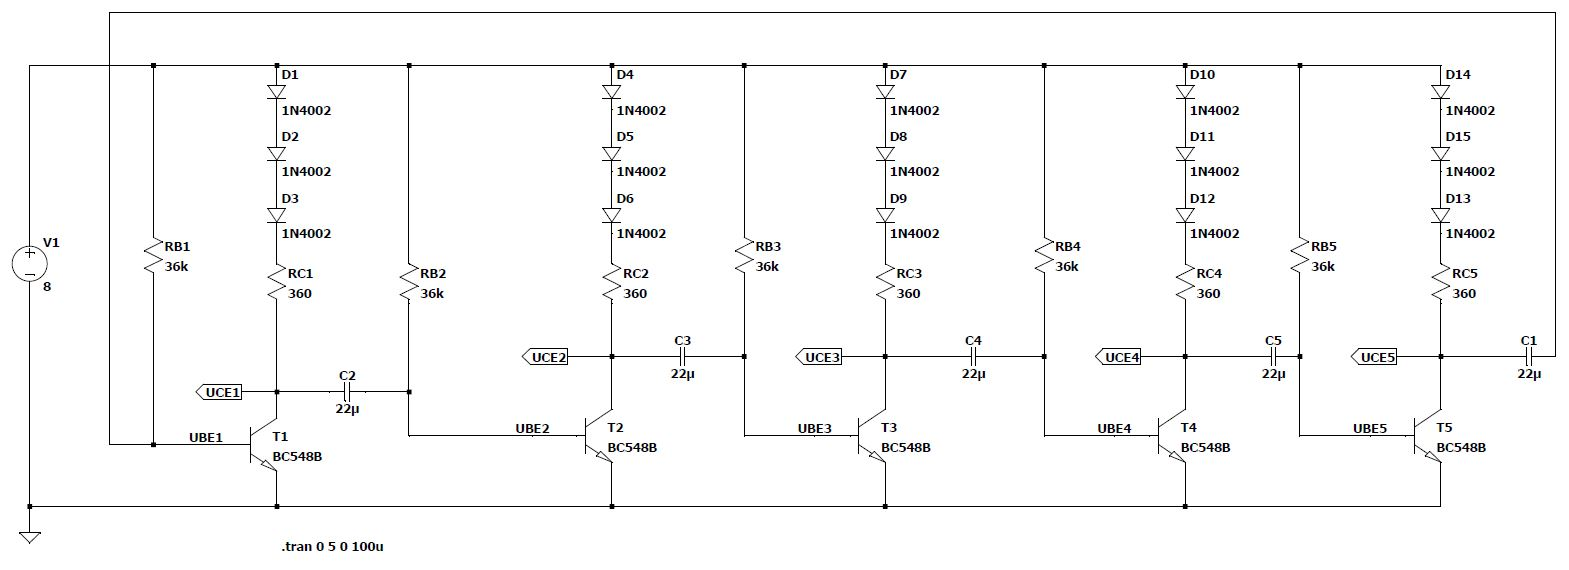
\includegraphics[width = \textwidth]{\figpath/Kipp_schem_5stufig.jpg}
    \caption{5 stufige Schaltung}
    \label{fig_Kap3_14:5stufig}
\end{figure}

\begin{figure}[H]
	\centering \small
	\scalebox{0.9}{% This file was created by matlab2tikz.
%
\definecolor{mycolor1}{rgb}{0.00000,0.44700,0.74100}%
\definecolor{mycolor2}{rgb}{0.85000,0.32500,0.09800}%
\definecolor{mycolor3}{rgb}{0.92900,0.69400,0.12500}%
\definecolor{mycolor4}{rgb}{0.49400,0.18400,0.55600}%
\definecolor{mycolor5}{rgb}{0.46600,0.67400,0.18800}%
%
\begin{tikzpicture}

\begin{axis}[%
width=4.521in,
height=3.555in,
at={(0.758in,0.481in)},
scale only axis,
xmin=0,
xmax=5,
xlabel style={font=\color{white!15!black}},
xlabel={$t \text{ in s}$},
ymin=-6,
ymax=1,
ylabel style={font=\color{white!15!black}},
ylabel={$U \text{ in V}$},
axis background/.style={fill=white},
title style={font=\bfseries},
title={$U_{BE}$},
xmajorgrids,
ymajorgrids,
legend style={legend cell align=left, align=left, draw=white!15!black}
]
\addplot [color=mycolor1]
  table[row sep=crcr]{%
0	0.74\\
0.01	0.74\\
0.02	0.74\\
0.03	0.74\\
0.04	0.74\\
0.05	0.74\\
0.06	0.74\\
0.07	0.74\\
0.08	0.74\\
0.09	0.74\\
0.1	0.74\\
0.11	0.74\\
0.12	0.74\\
0.13	0.74\\
0.14	0.74\\
0.15	0.75\\
0.16	-0.54\\
0.17	-0.5\\
0.18	-0.38\\
0.19	-0.25\\
0.2	-0.14\\
0.21	-0.02\\
0.22	0.08\\
0.23	0.18\\
0.24	0.29\\
0.25	0.38\\
0.26	0.48\\
0.27	0.58\\
0.28	0.67\\
0.29	0.74\\
0.3	0.74\\
0.31	0.74\\
0.32	0.74\\
0.33	0.74\\
0.34	0.74\\
0.35	0.74\\
0.36	0.74\\
0.37	0.74\\
0.38	0.74\\
0.39	0.74\\
0.4	0.74\\
0.41	0.74\\
0.42	0.74\\
0.43	0.74\\
0.44	0.74\\
0.45	0.74\\
0.46	0.74\\
0.47	0.74\\
0.48	0.74\\
0.49	0.74\\
0.5	0.76\\
0.51	0.75\\
0.52	0.74\\
0.53	0.74\\
0.54	0.74\\
0.55	0.74\\
0.56	0.74\\
0.57	0.74\\
0.58	0.74\\
0.59	0.74\\
0.6	0.74\\
0.61	0.74\\
0.62	0.74\\
0.63	0.74\\
0.64	0.74\\
0.65	0.74\\
0.66	0.74\\
0.67	0.74\\
0.68	0.74\\
0.69	0.74\\
0.7	0.74\\
0.71	0.74\\
0.72	0.74\\
0.73	0.74\\
0.74	0.74\\
0.75	0.74\\
0.76	0.74\\
0.77	0.74\\
0.78	0.74\\
0.79	0.74\\
0.8	0.74\\
0.81	0.74\\
0.82	0.74\\
0.83	0.74\\
0.84	0.74\\
0.85	0.74\\
0.86	0.74\\
0.87	0.74\\
0.88	0.74\\
0.89	0.74\\
0.9	0.74\\
0.91	0.74\\
0.92	0.74\\
0.93	0.74\\
0.94	0.74\\
0.95	0.74\\
0.96	0.74\\
0.97	0.74\\
0.98	0.74\\
0.99	0.74\\
1	0.74\\
1.01	0.17\\
1.02	-4.07\\
1.03	-5.81\\
1.04	-5.64\\
1.05	-5.47\\
1.06	-5.3\\
1.07	-5.13\\
1.08	-4.97\\
1.09	-4.8\\
1.1	-4.64\\
1.11	-4.48\\
1.12	-4.33\\
1.13	-4.17\\
1.14	-4.02\\
1.15	-3.87\\
1.16	-3.72\\
1.17	-3.57\\
1.18	-3.43\\
1.19	-3.28\\
1.2	-3.14\\
1.21	-3\\
1.22	-2.87\\
1.23	-2.73\\
1.24	-2.59\\
1.25	-2.46\\
1.26	-2.33\\
1.27	-2.2\\
1.28	-2.07\\
1.29	-1.95\\
1.3	-1.91\\
1.31	-1.76\\
1.32	-1.62\\
1.33	-1.49\\
1.34	-1.36\\
1.35	-1.24\\
1.36	-1.12\\
1.37	-1\\
1.38	-0.88\\
1.39	-0.77\\
1.4	-0.66\\
1.41	-0.55\\
1.42	-0.44\\
1.43	-0.34\\
1.44	-0.23\\
1.45	-0.13\\
1.46	-0.03\\
1.47	0.08\\
1.48	0.18\\
1.49	0.27\\
1.5	0.37\\
1.51	0.47\\
1.52	0.56\\
1.53	0.65\\
1.54	0.74\\
1.55	0.74\\
1.56	0.74\\
1.57	0.74\\
1.58	0.74\\
1.59	0.74\\
1.6	0.74\\
1.61	0.74\\
1.62	0.74\\
1.63	0.74\\
1.64	0.74\\
1.65	0.74\\
1.66	0.74\\
1.67	0.74\\
1.68	0.74\\
1.69	0.74\\
1.7	0.74\\
1.71	0.74\\
1.72	0.74\\
1.73	0.74\\
1.74	0.74\\
1.75	0.74\\
1.76	0.74\\
1.77	0.74\\
1.78	0.74\\
1.79	0.74\\
1.8	0.74\\
1.81	0.74\\
1.82	0.76\\
1.83	0.75\\
1.84	0.74\\
1.85	0.74\\
1.86	0.74\\
1.87	0.74\\
1.88	0.74\\
1.89	0.74\\
1.9	0.74\\
1.91	0.74\\
1.92	0.74\\
1.93	0.74\\
1.94	0.74\\
1.95	0.74\\
1.96	0.74\\
1.97	0.74\\
1.98	0.74\\
1.99	0.74\\
2	0.74\\
2.01	0.74\\
2.02	0.74\\
2.03	0.74\\
2.04	0.74\\
2.05	0.74\\
2.06	0.74\\
2.07	0.74\\
2.08	0.74\\
2.09	0.74\\
2.1	0.74\\
2.11	0.74\\
2.12	0.74\\
2.13	0.74\\
2.14	0.74\\
2.15	0.74\\
2.16	0.74\\
2.17	0.74\\
2.18	0.74\\
2.19	0.74\\
2.2	0.74\\
2.21	0.74\\
2.22	0.74\\
2.23	0.74\\
2.24	0.74\\
2.25	0.74\\
2.26	0.74\\
2.27	0.74\\
2.28	0.74\\
2.29	0.74\\
2.3	0.74\\
2.31	0.74\\
2.32	0.74\\
2.33	0.74\\
2.34	-1\\
2.35	-5.89\\
2.36	-5.72\\
2.37	-5.55\\
2.38	-5.38\\
2.39	-5.21\\
2.4	-5.04\\
2.41	-4.88\\
2.42	-4.72\\
2.43	-4.56\\
2.44	-4.4\\
2.45	-4.25\\
2.46	-4.09\\
2.47	-3.94\\
2.48	-3.79\\
2.49	-3.64\\
2.5	-3.5\\
2.51	-3.35\\
2.52	-3.21\\
2.53	-3.07\\
2.54	-2.93\\
2.55	-2.79\\
2.56	-2.67\\
2.57	-2.61\\
2.58	-2.46\\
2.59	-2.31\\
2.6	-2.16\\
2.61	-2.03\\
2.62	-1.9\\
2.63	-1.77\\
2.64	-1.64\\
2.65	-1.52\\
2.66	-1.4\\
2.67	-1.28\\
2.68	-1.16\\
2.69	-1.05\\
2.7	-0.93\\
2.71	-0.82\\
2.72	-0.71\\
2.73	-0.6\\
2.74	-0.49\\
2.75	-0.38\\
2.76	-0.28\\
2.77	-0.17\\
2.78	-0.07\\
2.79	0.03\\
2.8	0.13\\
2.81	0.23\\
2.82	0.33\\
2.83	0.42\\
2.84	0.52\\
2.85	0.61\\
2.86	0.7\\
2.87	0.74\\
2.88	0.74\\
2.89	0.74\\
2.9	0.74\\
2.91	0.74\\
2.92	0.74\\
2.93	0.74\\
2.94	0.74\\
2.95	0.74\\
2.96	0.74\\
2.97	0.74\\
2.98	0.74\\
2.99	0.74\\
3	0.74\\
3.01	0.74\\
3.02	0.74\\
3.03	0.74\\
3.04	0.74\\
3.05	0.74\\
3.06	0.74\\
3.07	0.74\\
3.08	0.74\\
3.09	0.76\\
3.1	0.75\\
3.11	0.74\\
3.12	0.74\\
3.13	0.74\\
3.14	0.74\\
3.15	0.74\\
3.16	0.74\\
3.17	0.74\\
3.18	0.74\\
3.19	0.74\\
3.2	0.74\\
3.21	0.74\\
3.22	0.74\\
3.23	0.74\\
3.24	0.74\\
3.25	0.74\\
3.26	0.74\\
3.27	0.74\\
3.28	0.74\\
3.29	0.74\\
3.3	0.74\\
3.31	0.74\\
3.32	0.74\\
3.33	0.74\\
3.34	0.74\\
3.35	0.74\\
3.36	0.74\\
3.37	0.74\\
3.38	0.74\\
3.39	0.74\\
3.4	0.74\\
3.41	0.74\\
3.42	0.74\\
3.43	0.74\\
3.44	0.74\\
3.45	0.74\\
3.46	0.74\\
3.47	0.74\\
3.48	0.74\\
3.49	0.74\\
3.5	0.74\\
3.51	0.74\\
3.52	0.74\\
3.53	0.74\\
3.54	0.74\\
3.55	0.74\\
3.56	0.74\\
3.57	0.74\\
3.58	0.74\\
3.59	0.74\\
3.6	0.74\\
3.61	-1.56\\
3.62	-5.87\\
3.63	-5.7\\
3.64	-5.53\\
3.65	-5.36\\
3.66	-5.19\\
3.67	-5.02\\
3.68	-4.86\\
3.69	-4.7\\
3.7	-4.54\\
3.71	-4.38\\
3.72	-4.23\\
3.73	-4.07\\
3.74	-3.92\\
3.75	-3.77\\
3.76	-3.62\\
3.77	-3.48\\
3.78	-3.33\\
3.79	-3.19\\
3.8	-3.05\\
3.81	-2.91\\
3.82	-2.78\\
3.83	-2.64\\
3.84	-2.51\\
3.85	-2.38\\
3.86	-2.25\\
3.87	-2.12\\
3.88	-1.99\\
3.89	-1.95\\
3.9	-1.81\\
3.91	-1.67\\
3.92	-1.53\\
3.93	-1.4\\
3.94	-1.28\\
3.95	-1.16\\
3.96	-1.04\\
3.97	-0.92\\
3.98	-0.81\\
3.99	-0.7\\
4	-0.59\\
4.01	-0.48\\
4.02	-0.37\\
4.03	-0.27\\
4.04	-0.16\\
4.05	-0.06\\
4.06	0.04\\
4.07	0.14\\
4.08	0.24\\
4.09	0.34\\
4.1	0.43\\
4.11	0.53\\
4.12	0.62\\
4.13	0.71\\
4.14	0.74\\
4.15	0.74\\
4.16	0.74\\
4.17	0.74\\
4.18	0.74\\
4.19	0.74\\
4.2	0.74\\
4.21	0.74\\
4.22	0.74\\
4.23	0.74\\
4.24	0.74\\
4.25	0.74\\
4.26	0.74\\
4.27	0.74\\
4.28	0.74\\
4.29	0.74\\
4.3	0.74\\
4.31	0.74\\
4.32	0.74\\
4.33	0.74\\
4.34	0.74\\
4.35	0.74\\
4.36	0.74\\
4.37	0.74\\
4.38	0.74\\
4.39	0.74\\
4.4	0.74\\
4.41	0.76\\
4.42	0.75\\
4.43	0.75\\
4.44	0.74\\
4.45	0.74\\
4.46	0.74\\
4.47	0.74\\
4.48	0.74\\
4.49	0.74\\
4.5	0.74\\
4.51	0.74\\
4.52	0.74\\
4.53	0.74\\
4.54	0.74\\
4.55	0.74\\
4.56	0.74\\
4.57	0.74\\
4.58	0.74\\
4.59	0.74\\
4.6	0.74\\
4.61	0.74\\
4.62	0.74\\
4.63	0.74\\
4.64	0.74\\
4.65	0.74\\
4.66	0.74\\
4.67	0.74\\
4.68	0.74\\
4.69	0.74\\
4.7	0.74\\
4.71	0.74\\
4.72	0.74\\
4.73	0.74\\
4.74	0.74\\
4.75	0.74\\
4.76	0.74\\
4.77	0.74\\
4.78	0.74\\
4.79	0.74\\
4.8	0.74\\
4.81	0.74\\
4.82	0.74\\
4.83	0.74\\
4.84	0.74\\
4.85	0.74\\
4.86	0.74\\
4.87	0.74\\
4.88	0.74\\
4.89	0.74\\
4.9	0.74\\
4.91	0.74\\
4.92	0.74\\
4.93	-0.18\\
4.94	-5.95\\
4.95	-5.77\\
4.96	-5.6\\
4.97	-5.43\\
4.98	-5.26\\
4.99	-5.1\\
5	-4.93\\
};
\addlegendentry{$\text{U}_{\text{BE1}}$}

\addplot [color=mycolor2]
  table[row sep=crcr]{%
0	0.74\\
0.01	0.74\\
0.02	0.74\\
0.03	0.74\\
0.04	0.74\\
0.05	0.74\\
0.06	0.74\\
0.07	0.74\\
0.08	0.74\\
0.09	0.74\\
0.1	0.74\\
0.11	0.74\\
0.12	0.74\\
0.13	0.74\\
0.14	0.74\\
0.15	0.74\\
0.16	0.76\\
0.17	0.75\\
0.18	0.74\\
0.19	0.74\\
0.2	0.74\\
0.21	0.74\\
0.22	0.74\\
0.23	0.74\\
0.24	0.74\\
0.25	0.74\\
0.26	0.74\\
0.27	0.74\\
0.28	-0.06\\
0.29	-5.65\\
0.3	-5.48\\
0.31	-5.31\\
0.32	-5.14\\
0.33	-4.97\\
0.34	-4.81\\
0.35	-4.65\\
0.36	-4.49\\
0.37	-4.34\\
0.38	-4.18\\
0.39	-4.03\\
0.4	-3.88\\
0.41	-3.73\\
0.42	-3.58\\
0.43	-3.44\\
0.44	-3.29\\
0.45	-3.15\\
0.46	-3.01\\
0.47	-2.87\\
0.48	-2.74\\
0.49	-2.61\\
0.5	-2.55\\
0.51	-2.4\\
0.52	-2.25\\
0.53	-2.11\\
0.54	-1.97\\
0.55	-1.84\\
0.56	-1.72\\
0.57	-1.59\\
0.58	-1.47\\
0.59	-1.35\\
0.6	-1.23\\
0.61	-1.11\\
0.62	-1\\
0.63	-0.89\\
0.64	-0.77\\
0.65	-0.66\\
0.66	-0.55\\
0.67	-0.45\\
0.68	-0.34\\
0.69	-0.24\\
0.7	-0.13\\
0.71	-0.03\\
0.72	0.07\\
0.73	0.17\\
0.74	0.27\\
0.75	0.37\\
0.76	0.46\\
0.77	0.56\\
0.78	0.65\\
0.79	0.74\\
0.8	0.74\\
0.81	0.74\\
0.82	0.74\\
0.83	0.74\\
0.84	0.74\\
0.85	0.74\\
0.86	0.74\\
0.87	0.74\\
0.88	0.74\\
0.89	0.74\\
0.9	0.74\\
0.91	0.74\\
0.92	0.74\\
0.93	0.74\\
0.94	0.74\\
0.95	0.74\\
0.96	0.74\\
0.97	0.74\\
0.98	0.74\\
0.99	0.74\\
1	0.74\\
1.01	0.77\\
1.02	0.75\\
1.03	0.75\\
1.04	0.74\\
1.05	0.74\\
1.06	0.74\\
1.07	0.74\\
1.08	0.74\\
1.09	0.74\\
1.1	0.74\\
1.11	0.74\\
1.12	0.74\\
1.13	0.74\\
1.14	0.74\\
1.15	0.74\\
1.16	0.74\\
1.17	0.74\\
1.18	0.74\\
1.19	0.74\\
1.2	0.74\\
1.21	0.74\\
1.22	0.74\\
1.23	0.74\\
1.24	0.74\\
1.25	0.74\\
1.26	0.74\\
1.27	0.74\\
1.28	0.74\\
1.29	0.74\\
1.3	0.74\\
1.31	0.74\\
1.32	0.74\\
1.33	0.74\\
1.34	0.74\\
1.35	0.74\\
1.36	0.74\\
1.37	0.74\\
1.38	0.74\\
1.39	0.74\\
1.4	0.74\\
1.41	0.74\\
1.42	0.74\\
1.43	0.74\\
1.44	0.74\\
1.45	0.74\\
1.46	0.74\\
1.47	0.74\\
1.48	0.74\\
1.49	0.74\\
1.5	0.74\\
1.51	0.74\\
1.52	0.74\\
1.53	-0.04\\
1.54	-5.57\\
1.55	-5.79\\
1.56	-5.61\\
1.57	-5.44\\
1.58	-5.28\\
1.59	-5.11\\
1.6	-4.94\\
1.61	-4.78\\
1.62	-4.62\\
1.63	-4.46\\
1.64	-4.31\\
1.65	-4.15\\
1.66	-4\\
1.67	-3.85\\
1.68	-3.7\\
1.69	-3.55\\
1.7	-3.41\\
1.71	-3.27\\
1.72	-3.12\\
1.73	-2.99\\
1.74	-2.85\\
1.75	-2.71\\
1.76	-2.58\\
1.77	-2.44\\
1.78	-2.31\\
1.79	-2.18\\
1.8	-2.06\\
1.81	-1.94\\
1.82	-1.89\\
1.83	-1.75\\
1.84	-1.61\\
1.85	-1.47\\
1.86	-1.34\\
1.87	-1.22\\
1.88	-1.1\\
1.89	-0.98\\
1.9	-0.87\\
1.91	-0.76\\
1.92	-0.65\\
1.93	-0.54\\
1.94	-0.43\\
1.95	-0.32\\
1.96	-0.22\\
1.97	-0.11\\
1.98	-0.01\\
1.99	0.09\\
2	0.19\\
2.01	0.29\\
2.02	0.38\\
2.03	0.48\\
2.04	0.57\\
2.05	0.67\\
2.06	0.74\\
2.07	0.74\\
2.08	0.74\\
2.09	0.74\\
2.1	0.74\\
2.11	0.74\\
2.12	0.74\\
2.13	0.74\\
2.14	0.74\\
2.15	0.74\\
2.16	0.74\\
2.17	0.74\\
2.18	0.74\\
2.19	0.74\\
2.2	0.74\\
2.21	0.74\\
2.22	0.74\\
2.23	0.74\\
2.24	0.74\\
2.25	0.74\\
2.26	0.74\\
2.27	0.74\\
2.28	0.74\\
2.29	0.74\\
2.3	0.74\\
2.31	0.74\\
2.32	0.74\\
2.33	0.74\\
2.34	0.76\\
2.35	0.75\\
2.36	0.74\\
2.37	0.74\\
2.38	0.74\\
2.39	0.74\\
2.4	0.74\\
2.41	0.74\\
2.42	0.74\\
2.43	0.74\\
2.44	0.74\\
2.45	0.74\\
2.46	0.74\\
2.47	0.74\\
2.48	0.74\\
2.49	0.74\\
2.5	0.74\\
2.51	0.74\\
2.52	0.74\\
2.53	0.74\\
2.54	0.74\\
2.55	0.74\\
2.56	0.74\\
2.57	0.74\\
2.58	0.74\\
2.59	0.74\\
2.6	0.74\\
2.61	0.74\\
2.62	0.74\\
2.63	0.74\\
2.64	0.74\\
2.65	0.74\\
2.66	0.74\\
2.67	0.74\\
2.68	0.74\\
2.69	0.74\\
2.7	0.74\\
2.71	0.74\\
2.72	0.74\\
2.73	0.74\\
2.74	0.74\\
2.75	0.74\\
2.76	0.74\\
2.77	0.74\\
2.78	0.74\\
2.79	0.74\\
2.8	0.74\\
2.81	0.74\\
2.82	0.74\\
2.83	0.74\\
2.84	0.74\\
2.85	0.74\\
2.86	-1.62\\
2.87	-5.87\\
2.88	-5.69\\
2.89	-5.52\\
2.9	-5.35\\
2.91	-5.19\\
2.92	-5.02\\
2.93	-4.86\\
2.94	-4.7\\
2.95	-4.54\\
2.96	-4.38\\
2.97	-4.22\\
2.98	-4.07\\
2.99	-3.92\\
3	-3.77\\
3.01	-3.62\\
3.02	-3.48\\
3.03	-3.33\\
3.04	-3.19\\
3.05	-3.05\\
3.06	-2.91\\
3.07	-2.77\\
3.08	-2.66\\
3.09	-2.59\\
3.1	-2.43\\
3.11	-2.29\\
3.12	-2.14\\
3.13	-2.01\\
3.14	-1.88\\
3.15	-1.75\\
3.16	-1.63\\
3.17	-1.5\\
3.18	-1.38\\
3.19	-1.26\\
3.2	-1.15\\
3.21	-1.03\\
3.22	-0.92\\
3.23	-0.8\\
3.24	-0.69\\
3.25	-0.58\\
3.26	-0.48\\
3.27	-0.37\\
3.28	-0.26\\
3.29	-0.16\\
3.3	-0.06\\
3.31	0.04\\
3.32	0.14\\
3.33	0.24\\
3.34	0.34\\
3.35	0.44\\
3.36	0.53\\
3.37	0.62\\
3.38	0.71\\
3.39	0.74\\
3.4	0.74\\
3.41	0.74\\
3.42	0.74\\
3.43	0.74\\
3.44	0.74\\
3.45	0.74\\
3.46	0.74\\
3.47	0.74\\
3.48	0.74\\
3.49	0.74\\
3.5	0.74\\
3.51	0.74\\
3.52	0.74\\
3.53	0.74\\
3.54	0.74\\
3.55	0.74\\
3.56	0.74\\
3.57	0.74\\
3.58	0.74\\
3.59	0.74\\
3.6	0.74\\
3.61	0.76\\
3.62	0.75\\
3.63	0.74\\
3.64	0.74\\
3.65	0.74\\
3.66	0.74\\
3.67	0.74\\
3.68	0.74\\
3.69	0.74\\
3.7	0.74\\
3.71	0.74\\
3.72	0.74\\
3.73	0.74\\
3.74	0.74\\
3.75	0.74\\
3.76	0.74\\
3.77	0.74\\
3.78	0.74\\
3.79	0.74\\
3.8	0.74\\
3.81	0.74\\
3.82	0.74\\
3.83	0.74\\
3.84	0.74\\
3.85	0.74\\
3.86	0.74\\
3.87	0.74\\
3.88	0.74\\
3.89	0.74\\
3.9	0.74\\
3.91	0.74\\
3.92	0.74\\
3.93	0.74\\
3.94	0.74\\
3.95	0.74\\
3.96	0.74\\
3.97	0.74\\
3.98	0.74\\
3.99	0.74\\
4	0.74\\
4.01	0.74\\
4.02	0.74\\
4.03	0.74\\
4.04	0.74\\
4.05	0.74\\
4.06	0.74\\
4.07	0.74\\
4.08	0.74\\
4.09	0.74\\
4.1	0.74\\
4.11	0.74\\
4.12	0.63\\
4.13	-2.34\\
4.14	-5.85\\
4.15	-5.67\\
4.16	-5.5\\
4.17	-5.33\\
4.18	-5.17\\
4.19	-5\\
4.2	-4.84\\
4.21	-4.68\\
4.22	-4.52\\
4.23	-4.36\\
4.24	-4.21\\
4.25	-4.05\\
4.26	-3.9\\
4.27	-3.75\\
4.28	-3.6\\
4.29	-3.46\\
4.3	-3.32\\
4.31	-3.17\\
4.32	-3.03\\
4.33	-2.89\\
4.34	-2.76\\
4.35	-2.62\\
4.36	-2.49\\
4.37	-2.36\\
4.38	-2.23\\
4.39	-2.1\\
4.4	-1.98\\
4.41	-1.93\\
4.42	-1.79\\
4.43	-1.65\\
4.44	-1.52\\
4.45	-1.39\\
4.46	-1.26\\
4.47	-1.14\\
4.48	-1.02\\
4.49	-0.91\\
4.5	-0.8\\
4.51	-0.68\\
4.52	-0.57\\
4.53	-0.47\\
4.54	-0.36\\
4.55	-0.25\\
4.56	-0.15\\
4.57	-0.05\\
4.58	0.05\\
4.59	0.15\\
4.6	0.25\\
4.61	0.35\\
4.62	0.45\\
4.63	0.54\\
4.64	0.63\\
4.65	0.72\\
4.66	0.74\\
4.67	0.74\\
4.68	0.74\\
4.69	0.74\\
4.7	0.74\\
4.71	0.74\\
4.72	0.74\\
4.73	0.74\\
4.74	0.74\\
4.75	0.74\\
4.76	0.74\\
4.77	0.74\\
4.78	0.74\\
4.79	0.74\\
4.8	0.74\\
4.81	0.74\\
4.82	0.74\\
4.83	0.74\\
4.84	0.74\\
4.85	0.74\\
4.86	0.74\\
4.87	0.74\\
4.88	0.74\\
4.89	0.74\\
4.9	0.74\\
4.91	0.74\\
4.92	0.74\\
4.93	0.76\\
4.94	0.75\\
4.95	0.74\\
4.96	0.74\\
4.97	0.74\\
4.98	0.74\\
4.99	0.74\\
5	0.74\\
};
\addlegendentry{$\text{U}_{\text{BE2}}$}

\addplot [color=mycolor3]
  table[row sep=crcr]{%
0	0.74\\
0.01	0.74\\
0.02	0.74\\
0.03	0.74\\
0.04	0.74\\
0.05	0.74\\
0.06	0.74\\
0.07	0.74\\
0.08	0.74\\
0.09	0.74\\
0.1	0.74\\
0.11	0.74\\
0.12	0.74\\
0.13	0.74\\
0.14	0.74\\
0.15	0.74\\
0.16	0.68\\
0.17	0.74\\
0.18	0.74\\
0.19	0.74\\
0.2	0.74\\
0.21	0.74\\
0.22	0.74\\
0.23	0.74\\
0.24	0.74\\
0.25	0.74\\
0.26	0.74\\
0.27	0.74\\
0.28	0.76\\
0.29	0.75\\
0.3	0.74\\
0.31	0.74\\
0.32	0.74\\
0.33	0.74\\
0.34	0.74\\
0.35	0.74\\
0.36	0.74\\
0.37	0.74\\
0.38	0.74\\
0.39	0.74\\
0.4	0.74\\
0.41	0.74\\
0.42	0.74\\
0.43	0.74\\
0.44	0.74\\
0.45	0.74\\
0.46	0.74\\
0.47	0.74\\
0.48	0.74\\
0.49	0.74\\
0.5	0.74\\
0.51	0.74\\
0.52	0.74\\
0.53	0.74\\
0.54	0.74\\
0.55	0.74\\
0.56	0.74\\
0.57	0.74\\
0.58	0.74\\
0.59	0.74\\
0.6	0.74\\
0.61	0.74\\
0.62	0.74\\
0.63	0.74\\
0.64	0.74\\
0.65	0.74\\
0.66	0.74\\
0.67	0.74\\
0.68	0.74\\
0.69	0.74\\
0.7	0.74\\
0.71	0.74\\
0.72	0.74\\
0.73	0.74\\
0.74	0.74\\
0.75	0.74\\
0.76	0.74\\
0.77	0.74\\
0.78	0.04\\
0.79	-5.05\\
0.8	-5.79\\
0.81	-5.62\\
0.82	-5.45\\
0.83	-5.28\\
0.84	-5.11\\
0.85	-4.95\\
0.86	-4.78\\
0.87	-4.62\\
0.88	-4.47\\
0.89	-4.31\\
0.9	-4.15\\
0.91	-4\\
0.92	-3.85\\
0.93	-3.7\\
0.94	-3.56\\
0.95	-3.41\\
0.96	-3.27\\
0.97	-3.13\\
0.98	-2.99\\
0.99	-2.85\\
1	-2.72\\
1.01	-2.67\\
1.02	-2.52\\
1.03	-2.37\\
1.04	-2.22\\
1.05	-2.08\\
1.06	-1.95\\
1.07	-1.82\\
1.08	-1.69\\
1.09	-1.57\\
1.1	-1.45\\
1.11	-1.33\\
1.12	-1.21\\
1.13	-1.09\\
1.14	-0.98\\
1.15	-0.87\\
1.16	-0.75\\
1.17	-0.64\\
1.18	-0.54\\
1.19	-0.43\\
1.2	-0.32\\
1.21	-0.22\\
1.22	-0.11\\
1.23	-0.01\\
1.24	0.09\\
1.25	0.19\\
1.26	0.29\\
1.27	0.38\\
1.28	0.48\\
1.29	0.57\\
1.3	0.67\\
1.31	0.74\\
1.32	0.74\\
1.33	0.74\\
1.34	0.74\\
1.35	0.74\\
1.36	0.74\\
1.37	0.74\\
1.38	0.74\\
1.39	0.74\\
1.4	0.74\\
1.41	0.74\\
1.42	0.74\\
1.43	0.74\\
1.44	0.74\\
1.45	0.74\\
1.46	0.74\\
1.47	0.74\\
1.48	0.74\\
1.49	0.74\\
1.5	0.74\\
1.51	0.74\\
1.52	0.74\\
1.53	0.76\\
1.54	0.75\\
1.55	0.75\\
1.56	0.74\\
1.57	0.74\\
1.58	0.74\\
1.59	0.74\\
1.6	0.74\\
1.61	0.74\\
1.62	0.74\\
1.63	0.74\\
1.64	0.74\\
1.65	0.74\\
1.66	0.74\\
1.67	0.74\\
1.68	0.74\\
1.69	0.74\\
1.7	0.74\\
1.71	0.74\\
1.72	0.74\\
1.73	0.74\\
1.74	0.74\\
1.75	0.74\\
1.76	0.74\\
1.77	0.74\\
1.78	0.74\\
1.79	0.74\\
1.8	0.74\\
1.81	0.74\\
1.82	0.74\\
1.83	0.74\\
1.84	0.74\\
1.85	0.74\\
1.86	0.74\\
1.87	0.74\\
1.88	0.74\\
1.89	0.74\\
1.9	0.74\\
1.91	0.74\\
1.92	0.74\\
1.93	0.74\\
1.94	0.74\\
1.95	0.74\\
1.96	0.74\\
1.97	0.74\\
1.98	0.74\\
1.99	0.74\\
2	0.74\\
2.01	0.74\\
2.02	0.74\\
2.03	0.74\\
2.04	0.74\\
2.05	-0.27\\
2.06	-5.94\\
2.07	-5.77\\
2.08	-5.59\\
2.09	-5.42\\
2.1	-5.25\\
2.11	-5.09\\
2.12	-4.92\\
2.13	-4.76\\
2.14	-4.6\\
2.15	-4.44\\
2.16	-4.29\\
2.17	-4.13\\
2.18	-3.98\\
2.19	-3.83\\
2.2	-3.68\\
2.21	-3.53\\
2.22	-3.39\\
2.23	-3.25\\
2.24	-3.11\\
2.25	-2.97\\
2.26	-2.83\\
2.27	-2.69\\
2.28	-2.56\\
2.29	-2.43\\
2.3	-2.3\\
2.31	-2.17\\
2.32	-2.04\\
2.33	-1.94\\
2.34	-1.87\\
2.35	-1.73\\
2.36	-1.59\\
2.37	-1.45\\
2.38	-1.33\\
2.39	-1.2\\
2.4	-1.09\\
2.41	-0.97\\
2.42	-0.86\\
2.43	-0.74\\
2.44	-0.63\\
2.45	-0.52\\
2.46	-0.42\\
2.47	-0.31\\
2.48	-0.2\\
2.49	-0.1\\
2.5	0\\
2.51	0.1\\
2.52	0.2\\
2.53	0.3\\
2.54	0.4\\
2.55	0.49\\
2.56	0.59\\
2.57	0.68\\
2.58	0.74\\
2.59	0.74\\
2.6	0.74\\
2.61	0.74\\
2.62	0.74\\
2.63	0.74\\
2.64	0.74\\
2.65	0.74\\
2.66	0.74\\
2.67	0.74\\
2.68	0.74\\
2.69	0.74\\
2.7	0.74\\
2.71	0.74\\
2.72	0.74\\
2.73	0.74\\
2.74	0.74\\
2.75	0.74\\
2.76	0.74\\
2.77	0.74\\
2.78	0.74\\
2.79	0.74\\
2.8	0.74\\
2.81	0.74\\
2.82	0.74\\
2.83	0.74\\
2.84	0.74\\
2.85	0.75\\
2.86	0.75\\
2.87	0.75\\
2.88	0.74\\
2.89	0.74\\
2.9	0.74\\
2.91	0.74\\
2.92	0.74\\
2.93	0.74\\
2.94	0.74\\
2.95	0.74\\
2.96	0.74\\
2.97	0.74\\
2.98	0.74\\
2.99	0.74\\
3	0.74\\
3.01	0.74\\
3.02	0.74\\
3.03	0.74\\
3.04	0.74\\
3.05	0.74\\
3.06	0.74\\
3.07	0.74\\
3.08	0.74\\
3.09	0.74\\
3.1	0.74\\
3.11	0.74\\
3.12	0.74\\
3.13	0.74\\
3.14	0.74\\
3.15	0.74\\
3.16	0.74\\
3.17	0.74\\
3.18	0.74\\
3.19	0.74\\
3.2	0.74\\
3.21	0.74\\
3.22	0.74\\
3.23	0.74\\
3.24	0.74\\
3.25	0.74\\
3.26	0.74\\
3.27	0.74\\
3.28	0.74\\
3.29	0.74\\
3.3	0.74\\
3.31	0.74\\
3.32	0.74\\
3.33	0.74\\
3.34	0.74\\
3.35	0.74\\
3.36	0.74\\
3.37	0.56\\
3.38	-2.46\\
3.39	-5.85\\
3.4	-5.67\\
3.41	-5.5\\
3.42	-5.33\\
3.43	-5.16\\
3.44	-5\\
3.45	-4.83\\
3.46	-4.67\\
3.47	-4.51\\
3.48	-4.36\\
3.49	-4.2\\
3.5	-4.05\\
3.51	-3.9\\
3.52	-3.75\\
3.53	-3.6\\
3.54	-3.46\\
3.55	-3.31\\
3.56	-3.17\\
3.57	-3.03\\
3.58	-2.89\\
3.59	-2.76\\
3.6	-2.67\\
3.61	-2.57\\
3.62	-2.41\\
3.63	-2.27\\
3.64	-2.13\\
3.65	-1.99\\
3.66	-1.86\\
3.67	-1.73\\
3.68	-1.61\\
3.69	-1.49\\
3.7	-1.37\\
3.71	-1.25\\
3.72	-1.13\\
3.73	-1.02\\
3.74	-0.9\\
3.75	-0.79\\
3.76	-0.68\\
3.77	-0.57\\
3.78	-0.46\\
3.79	-0.36\\
3.8	-0.25\\
3.81	-0.15\\
3.82	-0.04\\
3.83	0.06\\
3.84	0.16\\
3.85	0.26\\
3.86	0.35\\
3.87	0.45\\
3.88	0.54\\
3.89	0.64\\
3.9	0.72\\
3.91	0.74\\
3.92	0.74\\
3.93	0.74\\
3.94	0.74\\
3.95	0.74\\
3.96	0.74\\
3.97	0.74\\
3.98	0.74\\
3.99	0.74\\
4	0.74\\
4.01	0.74\\
4.02	0.74\\
4.03	0.74\\
4.04	0.74\\
4.05	0.74\\
4.06	0.74\\
4.07	0.74\\
4.08	0.74\\
4.09	0.74\\
4.1	0.74\\
4.11	0.74\\
4.12	0.77\\
4.13	0.75\\
4.14	0.75\\
4.15	0.74\\
4.16	0.74\\
4.17	0.74\\
4.18	0.74\\
4.19	0.74\\
4.2	0.74\\
4.21	0.74\\
4.22	0.74\\
4.23	0.74\\
4.24	0.74\\
4.25	0.74\\
4.26	0.74\\
4.27	0.74\\
4.28	0.74\\
4.29	0.74\\
4.3	0.74\\
4.31	0.74\\
4.32	0.74\\
4.33	0.74\\
4.34	0.74\\
4.35	0.74\\
4.36	0.74\\
4.37	0.74\\
4.38	0.74\\
4.39	0.74\\
4.4	0.74\\
4.41	0.74\\
4.42	0.74\\
4.43	0.74\\
4.44	0.74\\
4.45	0.74\\
4.46	0.74\\
4.47	0.74\\
4.48	0.74\\
4.49	0.74\\
4.5	0.74\\
4.51	0.74\\
4.52	0.74\\
4.53	0.74\\
4.54	0.74\\
4.55	0.74\\
4.56	0.74\\
4.57	0.74\\
4.58	0.74\\
4.59	0.74\\
4.6	0.74\\
4.61	0.74\\
4.62	0.74\\
4.63	0.74\\
4.64	0.29\\
4.65	-3.38\\
4.66	-5.83\\
4.67	-5.65\\
4.68	-5.48\\
4.69	-5.31\\
4.7	-5.14\\
4.71	-4.98\\
4.72	-4.82\\
4.73	-4.66\\
4.74	-4.5\\
4.75	-4.34\\
4.76	-4.19\\
4.77	-4.03\\
4.78	-3.88\\
4.79	-3.73\\
4.8	-3.59\\
4.81	-3.44\\
4.82	-3.3\\
4.83	-3.15\\
4.84	-3.01\\
4.85	-2.88\\
4.86	-2.74\\
4.87	-2.61\\
4.88	-2.47\\
4.89	-2.34\\
4.9	-2.21\\
4.91	-2.08\\
4.92	-1.96\\
4.93	-1.92\\
4.94	-1.78\\
4.95	-1.63\\
4.96	-1.5\\
4.97	-1.37\\
4.98	-1.25\\
4.99	-1.13\\
5	-1.01\\
};
\addlegendentry{$\text{U}_{\text{BE3}}$}

\addplot [color=mycolor4]
  table[row sep=crcr]{%
0	0.74\\
0.01	0.74\\
0.02	0.74\\
0.03	0.74\\
0.04	0.74\\
0.05	0.74\\
0.06	0.74\\
0.07	0.74\\
0.08	0.74\\
0.09	0.74\\
0.1	0.74\\
0.11	0.74\\
0.12	0.74\\
0.13	0.74\\
0.14	0.74\\
0.15	0.75\\
0.16	0.75\\
0.17	-3.11\\
0.18	-2.97\\
0.19	-2.83\\
0.2	-2.69\\
0.21	-2.56\\
0.22	-2.43\\
0.23	-2.29\\
0.24	-2.17\\
0.25	-2.04\\
0.26	-1.91\\
0.27	-1.79\\
0.28	-1.75\\
0.29	-1.61\\
0.3	-1.47\\
0.31	-1.34\\
0.32	-1.21\\
0.33	-1.09\\
0.34	-0.97\\
0.35	-0.86\\
0.36	-0.74\\
0.37	-0.63\\
0.38	-0.52\\
0.39	-0.41\\
0.4	-0.31\\
0.41	-0.2\\
0.42	-0.1\\
0.43	0\\
0.44	0.1\\
0.45	0.2\\
0.46	0.3\\
0.47	0.4\\
0.48	0.49\\
0.49	0.59\\
0.5	0.68\\
0.51	0.74\\
0.52	0.74\\
0.53	0.74\\
0.54	0.74\\
0.55	0.74\\
0.56	0.74\\
0.57	0.74\\
0.58	0.74\\
0.59	0.74\\
0.6	0.74\\
0.61	0.74\\
0.62	0.74\\
0.63	0.74\\
0.64	0.74\\
0.65	0.74\\
0.66	0.74\\
0.67	0.74\\
0.68	0.74\\
0.69	0.74\\
0.7	0.74\\
0.71	0.74\\
0.72	0.74\\
0.73	0.74\\
0.74	0.74\\
0.75	0.74\\
0.76	0.74\\
0.77	0.74\\
0.78	0.76\\
0.79	0.75\\
0.8	0.75\\
0.81	0.74\\
0.82	0.74\\
0.83	0.74\\
0.84	0.74\\
0.85	0.74\\
0.86	0.74\\
0.87	0.74\\
0.88	0.74\\
0.89	0.74\\
0.9	0.74\\
0.91	0.74\\
0.92	0.74\\
0.93	0.74\\
0.94	0.74\\
0.95	0.74\\
0.96	0.74\\
0.97	0.74\\
0.98	0.74\\
0.99	0.74\\
1	0.74\\
1.01	0.74\\
1.02	0.74\\
1.03	0.74\\
1.04	0.74\\
1.05	0.74\\
1.06	0.74\\
1.07	0.74\\
1.08	0.74\\
1.09	0.74\\
1.1	0.74\\
1.11	0.74\\
1.12	0.74\\
1.13	0.74\\
1.14	0.74\\
1.15	0.74\\
1.16	0.74\\
1.17	0.74\\
1.18	0.74\\
1.19	0.74\\
1.2	0.74\\
1.21	0.74\\
1.22	0.74\\
1.23	0.74\\
1.24	0.74\\
1.25	0.74\\
1.26	0.74\\
1.27	0.74\\
1.28	0.74\\
1.29	0.74\\
1.3	-0.25\\
1.31	-5.94\\
1.32	-5.77\\
1.33	-5.59\\
1.34	-5.42\\
1.35	-5.25\\
1.36	-5.09\\
1.37	-4.92\\
1.38	-4.76\\
1.39	-4.6\\
1.4	-4.44\\
1.41	-4.29\\
1.42	-4.13\\
1.43	-3.98\\
1.44	-3.83\\
1.45	-3.68\\
1.46	-3.54\\
1.47	-3.39\\
1.48	-3.25\\
1.49	-3.11\\
1.5	-2.97\\
1.51	-2.83\\
1.52	-2.7\\
1.53	-2.65\\
1.54	-2.5\\
1.55	-2.35\\
1.56	-2.2\\
1.57	-2.06\\
1.58	-1.93\\
1.59	-1.8\\
1.6	-1.68\\
1.61	-1.55\\
1.62	-1.43\\
1.63	-1.31\\
1.64	-1.19\\
1.65	-1.08\\
1.66	-0.96\\
1.67	-0.85\\
1.68	-0.74\\
1.69	-0.63\\
1.7	-0.52\\
1.71	-0.41\\
1.72	-0.31\\
1.73	-0.2\\
1.74	-0.1\\
1.75	0\\
1.76	0.1\\
1.77	0.2\\
1.78	0.3\\
1.79	0.4\\
1.8	0.49\\
1.81	0.59\\
1.82	0.68\\
1.83	0.74\\
1.84	0.74\\
1.85	0.74\\
1.86	0.74\\
1.87	0.74\\
1.88	0.74\\
1.89	0.74\\
1.9	0.74\\
1.91	0.74\\
1.92	0.74\\
1.93	0.74\\
1.94	0.74\\
1.95	0.74\\
1.96	0.74\\
1.97	0.74\\
1.98	0.74\\
1.99	0.74\\
2	0.74\\
2.01	0.74\\
2.02	0.74\\
2.03	0.74\\
2.04	0.74\\
2.05	0.76\\
2.06	0.75\\
2.07	0.74\\
2.08	0.74\\
2.09	0.74\\
2.1	0.74\\
2.11	0.74\\
2.12	0.74\\
2.13	0.74\\
2.14	0.74\\
2.15	0.74\\
2.16	0.74\\
2.17	0.74\\
2.18	0.74\\
2.19	0.74\\
2.2	0.74\\
2.21	0.74\\
2.22	0.74\\
2.23	0.74\\
2.24	0.74\\
2.25	0.74\\
2.26	0.74\\
2.27	0.74\\
2.28	0.74\\
2.29	0.74\\
2.3	0.74\\
2.31	0.74\\
2.32	0.74\\
2.33	0.74\\
2.34	0.74\\
2.35	0.74\\
2.36	0.74\\
2.37	0.74\\
2.38	0.74\\
2.39	0.74\\
2.4	0.74\\
2.41	0.74\\
2.42	0.74\\
2.43	0.74\\
2.44	0.74\\
2.45	0.74\\
2.46	0.74\\
2.47	0.74\\
2.48	0.74\\
2.49	0.74\\
2.5	0.74\\
2.51	0.74\\
2.52	0.74\\
2.53	0.74\\
2.54	0.74\\
2.55	0.74\\
2.56	0.74\\
2.57	-0.57\\
2.58	-5.92\\
2.59	-5.74\\
2.6	-5.57\\
2.61	-5.4\\
2.62	-5.23\\
2.63	-5.07\\
2.64	-4.9\\
2.65	-4.74\\
2.66	-4.58\\
2.67	-4.42\\
2.68	-4.27\\
2.69	-4.11\\
2.7	-3.96\\
2.71	-3.81\\
2.72	-3.66\\
2.73	-3.52\\
2.74	-3.37\\
2.75	-3.23\\
2.76	-3.09\\
2.77	-2.95\\
2.78	-2.81\\
2.79	-2.68\\
2.8	-2.54\\
2.81	-2.41\\
2.82	-2.28\\
2.83	-2.15\\
2.84	-2.02\\
2.85	-1.95\\
2.86	-1.85\\
2.87	-1.71\\
2.88	-1.57\\
2.89	-1.44\\
2.9	-1.31\\
2.91	-1.19\\
2.92	-1.07\\
2.93	-0.95\\
2.94	-0.84\\
2.95	-0.73\\
2.96	-0.62\\
2.97	-0.51\\
2.98	-0.4\\
2.99	-0.3\\
3	-0.19\\
3.01	-0.09\\
3.02	0.01\\
3.03	0.11\\
3.04	0.21\\
3.05	0.31\\
3.06	0.41\\
3.07	0.5\\
3.08	0.6\\
3.09	0.69\\
3.1	0.74\\
3.11	0.74\\
3.12	0.74\\
3.13	0.74\\
3.14	0.74\\
3.15	0.74\\
3.16	0.74\\
3.17	0.74\\
3.18	0.74\\
3.19	0.74\\
3.2	0.74\\
3.21	0.74\\
3.22	0.74\\
3.23	0.74\\
3.24	0.74\\
3.25	0.74\\
3.26	0.74\\
3.27	0.74\\
3.28	0.74\\
3.29	0.74\\
3.3	0.74\\
3.31	0.74\\
3.32	0.74\\
3.33	0.74\\
3.34	0.74\\
3.35	0.74\\
3.36	0.74\\
3.37	0.77\\
3.38	0.75\\
3.39	0.75\\
3.4	0.74\\
3.41	0.74\\
3.42	0.74\\
3.43	0.74\\
3.44	0.74\\
3.45	0.74\\
3.46	0.74\\
3.47	0.74\\
3.48	0.74\\
3.49	0.74\\
3.5	0.74\\
3.51	0.74\\
3.52	0.74\\
3.53	0.74\\
3.54	0.74\\
3.55	0.74\\
3.56	0.74\\
3.57	0.74\\
3.58	0.74\\
3.59	0.74\\
3.6	0.74\\
3.61	0.74\\
3.62	0.74\\
3.63	0.74\\
3.64	0.74\\
3.65	0.74\\
3.66	0.74\\
3.67	0.74\\
3.68	0.74\\
3.69	0.74\\
3.7	0.74\\
3.71	0.74\\
3.72	0.74\\
3.73	0.74\\
3.74	0.74\\
3.75	0.74\\
3.76	0.74\\
3.77	0.74\\
3.78	0.74\\
3.79	0.74\\
3.8	0.74\\
3.81	0.74\\
3.82	0.74\\
3.83	0.74\\
3.84	0.74\\
3.85	0.74\\
3.86	0.74\\
3.87	0.74\\
3.88	0.74\\
3.89	0.25\\
3.9	-3.58\\
3.91	-5.82\\
3.92	-5.65\\
3.93	-5.48\\
3.94	-5.31\\
3.95	-5.14\\
3.96	-4.98\\
3.97	-4.81\\
3.98	-4.65\\
3.99	-4.49\\
4	-4.34\\
4.01	-4.18\\
4.02	-4.03\\
4.03	-3.88\\
4.04	-3.73\\
4.05	-3.58\\
4.06	-3.44\\
4.07	-3.29\\
4.08	-3.15\\
4.09	-3.01\\
4.1	-2.87\\
4.11	-2.74\\
4.12	-2.69\\
4.13	-2.54\\
4.14	-2.39\\
4.15	-2.25\\
4.16	-2.11\\
4.17	-1.97\\
4.18	-1.84\\
4.19	-1.72\\
4.2	-1.59\\
4.21	-1.47\\
4.22	-1.35\\
4.23	-1.23\\
4.24	-1.11\\
4.25	-1\\
4.26	-0.89\\
4.27	-0.77\\
4.28	-0.66\\
4.29	-0.55\\
4.3	-0.45\\
4.31	-0.34\\
4.32	-0.24\\
4.33	-0.13\\
4.34	-0.03\\
4.35	0.07\\
4.36	0.17\\
4.37	0.27\\
4.38	0.37\\
4.39	0.46\\
4.4	0.56\\
4.41	0.65\\
4.42	0.74\\
4.43	0.74\\
4.44	0.74\\
4.45	0.74\\
4.46	0.74\\
4.47	0.74\\
4.48	0.74\\
4.49	0.74\\
4.5	0.74\\
4.51	0.74\\
4.52	0.74\\
4.53	0.74\\
4.54	0.74\\
4.55	0.74\\
4.56	0.74\\
4.57	0.74\\
4.58	0.74\\
4.59	0.74\\
4.6	0.74\\
4.61	0.74\\
4.62	0.74\\
4.63	0.74\\
4.64	0.77\\
4.65	0.75\\
4.66	0.75\\
4.67	0.74\\
4.68	0.74\\
4.69	0.74\\
4.7	0.74\\
4.71	0.74\\
4.72	0.74\\
4.73	0.74\\
4.74	0.74\\
4.75	0.74\\
4.76	0.74\\
4.77	0.74\\
4.78	0.74\\
4.79	0.74\\
4.8	0.74\\
4.81	0.74\\
4.82	0.74\\
4.83	0.74\\
4.84	0.74\\
4.85	0.74\\
4.86	0.74\\
4.87	0.74\\
4.88	0.74\\
4.89	0.74\\
4.9	0.74\\
4.91	0.74\\
4.92	0.74\\
4.93	0.74\\
4.94	0.74\\
4.95	0.74\\
4.96	0.74\\
4.97	0.74\\
4.98	0.74\\
4.99	0.74\\
5	0.74\\
};
\addlegendentry{$\text{U}_{\text{BE4}}$}

\addplot [color=mycolor5]
  table[row sep=crcr]{%
0	0.74\\
0.01	0.74\\
0.02	0.74\\
0.03	0.74\\
0.04	0.74\\
0.05	0.74\\
0.06	0.74\\
0.07	0.74\\
0.08	0.74\\
0.09	0.74\\
0.1	0.74\\
0.11	0.74\\
0.12	0.74\\
0.13	0.74\\
0.14	0.74\\
0.15	0.73\\
0.16	0.74\\
0.17	0.76\\
0.18	0.75\\
0.19	0.74\\
0.2	0.74\\
0.21	0.74\\
0.22	0.74\\
0.23	0.74\\
0.24	0.74\\
0.25	0.74\\
0.26	0.74\\
0.27	0.74\\
0.28	0.74\\
0.29	0.74\\
0.3	0.74\\
0.31	0.74\\
0.32	0.74\\
0.33	0.74\\
0.34	0.74\\
0.35	0.74\\
0.36	0.74\\
0.37	0.74\\
0.38	0.74\\
0.39	0.74\\
0.4	0.74\\
0.41	0.74\\
0.42	0.74\\
0.43	0.74\\
0.44	0.74\\
0.45	0.74\\
0.46	0.74\\
0.47	0.74\\
0.48	0.74\\
0.49	0.74\\
0.5	-0.53\\
0.51	-5.84\\
0.52	-5.66\\
0.53	-5.49\\
0.54	-5.32\\
0.55	-5.15\\
0.56	-4.99\\
0.57	-4.83\\
0.58	-4.66\\
0.59	-4.51\\
0.6	-4.35\\
0.61	-4.19\\
0.62	-4.04\\
0.63	-3.89\\
0.64	-3.74\\
0.65	-3.59\\
0.66	-3.45\\
0.67	-3.3\\
0.68	-3.16\\
0.69	-3.02\\
0.7	-2.88\\
0.71	-2.75\\
0.72	-2.61\\
0.73	-2.48\\
0.74	-2.35\\
0.75	-2.22\\
0.76	-2.09\\
0.77	-1.97\\
0.78	-1.93\\
0.79	-1.79\\
0.8	-1.64\\
0.81	-1.51\\
0.82	-1.38\\
0.83	-1.25\\
0.84	-1.13\\
0.85	-1.02\\
0.86	-0.9\\
0.87	-0.79\\
0.88	-0.68\\
0.89	-0.57\\
0.9	-0.46\\
0.91	-0.35\\
0.92	-0.25\\
0.93	-0.14\\
0.94	-0.04\\
0.95	0.06\\
0.96	0.16\\
0.97	0.26\\
0.98	0.36\\
0.99	0.45\\
1	0.55\\
1.01	0.64\\
1.02	0.73\\
1.03	0.74\\
1.04	0.74\\
1.05	0.74\\
1.06	0.74\\
1.07	0.74\\
1.08	0.74\\
1.09	0.74\\
1.1	0.74\\
1.11	0.74\\
1.12	0.74\\
1.13	0.74\\
1.14	0.74\\
1.15	0.74\\
1.16	0.74\\
1.17	0.74\\
1.18	0.74\\
1.19	0.74\\
1.2	0.74\\
1.21	0.74\\
1.22	0.74\\
1.23	0.74\\
1.24	0.74\\
1.25	0.74\\
1.26	0.74\\
1.27	0.74\\
1.28	0.74\\
1.29	0.74\\
1.3	0.76\\
1.31	0.75\\
1.32	0.74\\
1.33	0.74\\
1.34	0.74\\
1.35	0.74\\
1.36	0.74\\
1.37	0.74\\
1.38	0.74\\
1.39	0.74\\
1.4	0.74\\
1.41	0.74\\
1.42	0.74\\
1.43	0.74\\
1.44	0.74\\
1.45	0.74\\
1.46	0.74\\
1.47	0.74\\
1.48	0.74\\
1.49	0.74\\
1.5	0.74\\
1.51	0.74\\
1.52	0.74\\
1.53	0.74\\
1.54	0.74\\
1.55	0.74\\
1.56	0.74\\
1.57	0.74\\
1.58	0.74\\
1.59	0.74\\
1.6	0.74\\
1.61	0.74\\
1.62	0.74\\
1.63	0.74\\
1.64	0.74\\
1.65	0.74\\
1.66	0.74\\
1.67	0.74\\
1.68	0.74\\
1.69	0.74\\
1.7	0.74\\
1.71	0.74\\
1.72	0.74\\
1.73	0.74\\
1.74	0.74\\
1.75	0.74\\
1.76	0.74\\
1.77	0.74\\
1.78	0.74\\
1.79	0.74\\
1.8	0.74\\
1.81	0.74\\
1.82	-0.57\\
1.83	-5.92\\
1.84	-5.74\\
1.85	-5.57\\
1.86	-5.4\\
1.87	-5.23\\
1.88	-5.07\\
1.89	-4.9\\
1.9	-4.74\\
1.91	-4.58\\
1.92	-4.42\\
1.93	-4.27\\
1.94	-4.11\\
1.95	-3.96\\
1.96	-3.81\\
1.97	-3.66\\
1.98	-3.52\\
1.99	-3.37\\
2	-3.23\\
2.01	-3.09\\
2.02	-2.95\\
2.03	-2.81\\
2.04	-2.68\\
2.05	-2.63\\
2.06	-2.48\\
2.07	-2.33\\
2.08	-2.18\\
2.09	-2.05\\
2.1	-1.91\\
2.11	-1.78\\
2.12	-1.66\\
2.13	-1.54\\
2.14	-1.41\\
2.15	-1.3\\
2.16	-1.18\\
2.17	-1.06\\
2.18	-0.95\\
2.19	-0.84\\
2.2	-0.72\\
2.21	-0.61\\
2.22	-0.51\\
2.23	-0.4\\
2.24	-0.29\\
2.25	-0.19\\
2.26	-0.09\\
2.27	0.02\\
2.28	0.12\\
2.29	0.22\\
2.3	0.31\\
2.31	0.41\\
2.32	0.5\\
2.33	0.6\\
2.34	0.69\\
2.35	0.74\\
2.36	0.74\\
2.37	0.74\\
2.38	0.74\\
2.39	0.74\\
2.4	0.74\\
2.41	0.74\\
2.42	0.74\\
2.43	0.74\\
2.44	0.74\\
2.45	0.74\\
2.46	0.74\\
2.47	0.74\\
2.48	0.74\\
2.49	0.74\\
2.5	0.74\\
2.51	0.74\\
2.52	0.74\\
2.53	0.74\\
2.54	0.74\\
2.55	0.74\\
2.56	0.74\\
2.57	0.76\\
2.58	0.75\\
2.59	0.74\\
2.6	0.74\\
2.61	0.74\\
2.62	0.74\\
2.63	0.74\\
2.64	0.74\\
2.65	0.74\\
2.66	0.74\\
2.67	0.74\\
2.68	0.74\\
2.69	0.74\\
2.7	0.74\\
2.71	0.74\\
2.72	0.74\\
2.73	0.74\\
2.74	0.74\\
2.75	0.74\\
2.76	0.74\\
2.77	0.74\\
2.78	0.74\\
2.79	0.74\\
2.8	0.74\\
2.81	0.74\\
2.82	0.74\\
2.83	0.74\\
2.84	0.74\\
2.85	0.74\\
2.86	0.74\\
2.87	0.74\\
2.88	0.74\\
2.89	0.74\\
2.9	0.74\\
2.91	0.74\\
2.92	0.74\\
2.93	0.74\\
2.94	0.74\\
2.95	0.74\\
2.96	0.74\\
2.97	0.74\\
2.98	0.74\\
2.99	0.74\\
3	0.74\\
3.01	0.74\\
3.02	0.74\\
3.03	0.74\\
3.04	0.74\\
3.05	0.74\\
3.06	0.74\\
3.07	0.74\\
3.08	0.74\\
3.09	-0.98\\
3.1	-5.89\\
3.11	-5.72\\
3.12	-5.55\\
3.13	-5.38\\
3.14	-5.21\\
3.15	-5.04\\
3.16	-4.88\\
3.17	-4.72\\
3.18	-4.56\\
3.19	-4.4\\
3.2	-4.25\\
3.21	-4.09\\
3.22	-3.94\\
3.23	-3.79\\
3.24	-3.64\\
3.25	-3.5\\
3.26	-3.35\\
3.27	-3.21\\
3.28	-3.07\\
3.29	-2.93\\
3.3	-2.79\\
3.31	-2.66\\
3.32	-2.52\\
3.33	-2.39\\
3.34	-2.26\\
3.35	-2.13\\
3.36	-2.01\\
3.37	-1.97\\
3.38	-1.83\\
3.39	-1.69\\
3.4	-1.55\\
3.41	-1.42\\
3.42	-1.29\\
3.43	-1.17\\
3.44	-1.06\\
3.45	-0.94\\
3.46	-0.83\\
3.47	-0.71\\
3.48	-0.6\\
3.49	-0.49\\
3.5	-0.39\\
3.51	-0.28\\
3.52	-0.18\\
3.53	-0.07\\
3.54	0.03\\
3.55	0.13\\
3.56	0.23\\
3.57	0.32\\
3.58	0.42\\
3.59	0.52\\
3.6	0.61\\
3.61	0.7\\
3.62	0.74\\
3.63	0.74\\
3.64	0.74\\
3.65	0.74\\
3.66	0.74\\
3.67	0.74\\
3.68	0.74\\
3.69	0.74\\
3.7	0.74\\
3.71	0.74\\
3.72	0.74\\
3.73	0.74\\
3.74	0.74\\
3.75	0.74\\
3.76	0.74\\
3.77	0.74\\
3.78	0.74\\
3.79	0.74\\
3.8	0.74\\
3.81	0.74\\
3.82	0.74\\
3.83	0.74\\
3.84	0.74\\
3.85	0.74\\
3.86	0.74\\
3.87	0.74\\
3.88	0.74\\
3.89	0.77\\
3.9	0.75\\
3.91	0.75\\
3.92	0.74\\
3.93	0.74\\
3.94	0.74\\
3.95	0.74\\
3.96	0.74\\
3.97	0.74\\
3.98	0.74\\
3.99	0.74\\
4	0.74\\
4.01	0.74\\
4.02	0.74\\
4.03	0.74\\
4.04	0.74\\
4.05	0.74\\
4.06	0.74\\
4.07	0.74\\
4.08	0.74\\
4.09	0.74\\
4.1	0.74\\
4.11	0.74\\
4.12	0.74\\
4.13	0.74\\
4.14	0.74\\
4.15	0.74\\
4.16	0.74\\
4.17	0.74\\
4.18	0.74\\
4.19	0.74\\
4.2	0.74\\
4.21	0.74\\
4.22	0.74\\
4.23	0.74\\
4.24	0.74\\
4.25	0.74\\
4.26	0.74\\
4.27	0.74\\
4.28	0.74\\
4.29	0.74\\
4.3	0.74\\
4.31	0.74\\
4.32	0.74\\
4.33	0.74\\
4.34	0.74\\
4.35	0.74\\
4.36	0.74\\
4.37	0.74\\
4.38	0.74\\
4.39	0.74\\
4.4	0.74\\
4.41	0.05\\
4.42	-4.96\\
4.43	-5.8\\
4.44	-5.62\\
4.45	-5.45\\
4.46	-5.28\\
4.47	-5.12\\
4.48	-4.95\\
4.49	-4.79\\
4.5	-4.63\\
4.51	-4.47\\
4.52	-4.32\\
4.53	-4.16\\
4.54	-4.01\\
4.55	-3.86\\
4.56	-3.71\\
4.57	-3.56\\
4.58	-3.42\\
4.59	-3.27\\
4.6	-3.13\\
4.61	-2.99\\
4.62	-2.85\\
4.63	-2.72\\
4.64	-2.67\\
4.65	-2.52\\
4.66	-2.37\\
4.67	-2.23\\
4.68	-2.09\\
4.69	-1.95\\
4.7	-1.82\\
4.71	-1.7\\
4.72	-1.57\\
4.73	-1.45\\
4.74	-1.33\\
4.75	-1.22\\
4.76	-1.1\\
4.77	-0.98\\
4.78	-0.87\\
4.79	-0.76\\
4.8	-0.65\\
4.81	-0.54\\
4.82	-0.43\\
4.83	-0.33\\
4.84	-0.22\\
4.85	-0.12\\
4.86	-0.02\\
4.87	0.08\\
4.88	0.18\\
4.89	0.28\\
4.9	0.38\\
4.91	0.47\\
4.92	0.57\\
4.93	0.66\\
4.94	0.74\\
4.95	0.74\\
4.96	0.74\\
4.97	0.74\\
4.98	0.74\\
4.99	0.74\\
5	0.74\\
};
\addlegendentry{$\text{U}_{\text{BE5}}$}

\end{axis}
\end{tikzpicture}%}
	\caption{Basis-Emitter-Spannungen des 5-Stufigen LED-Blinklichts}
	\label{fig_Kap3_15:Spannungen}
\end{figure}